% Created by tikzDevice version 0.12.6 on 2025-01-20 18:04:58
% !TEX encoding = UTF-8 Unicode
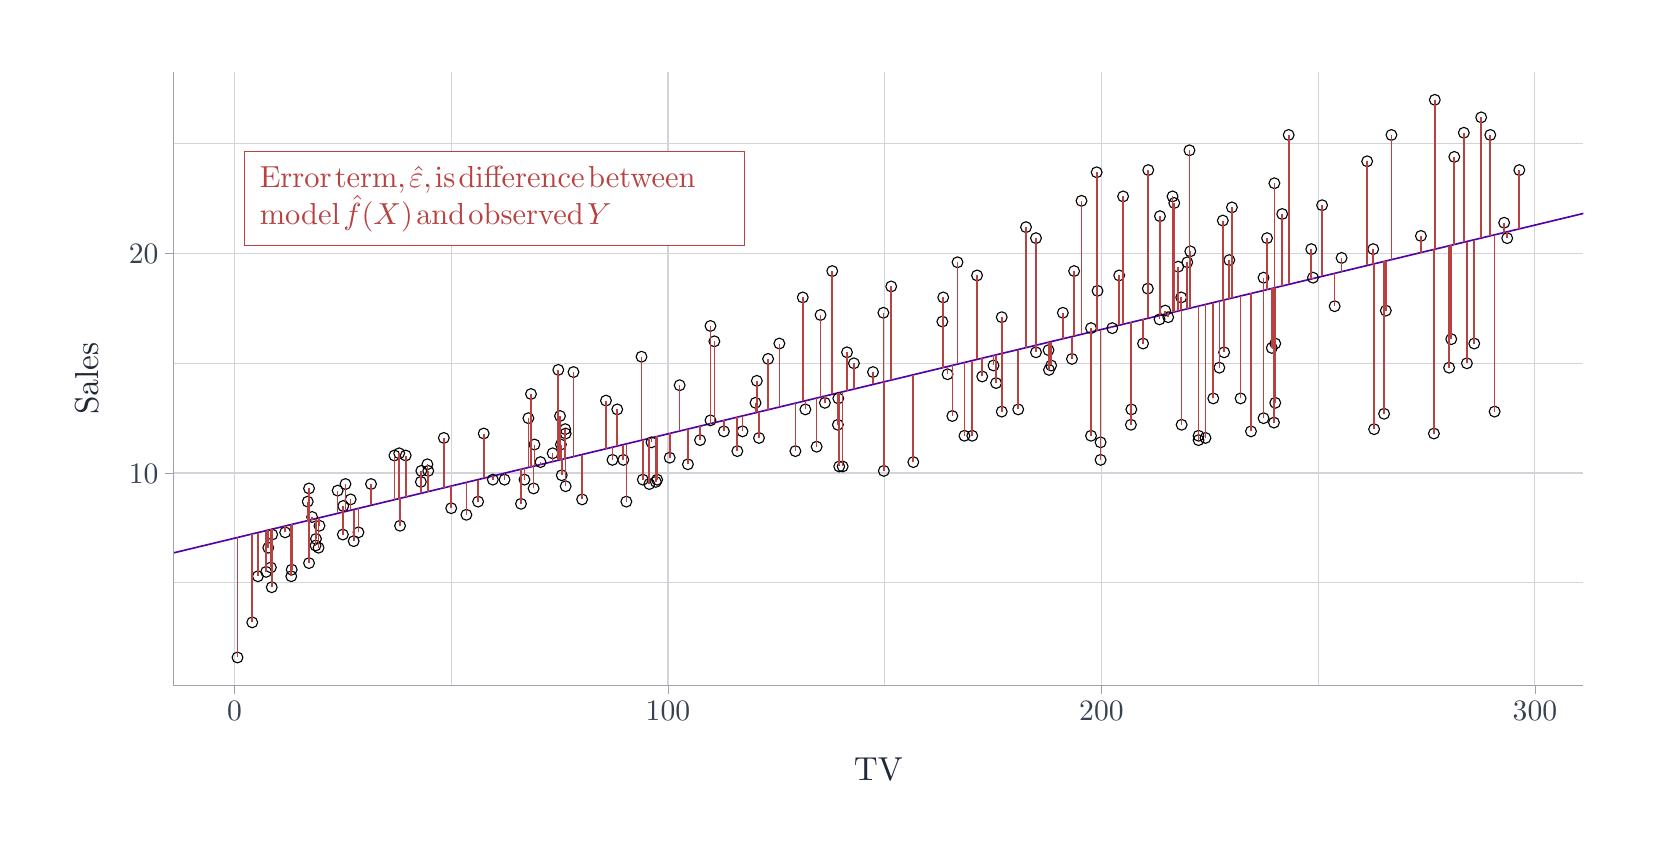
\begin{tikzpicture}[x=1pt,y=1pt]
\definecolor{fillColor}{RGB}{255,255,255}
\path[use as bounding box,fill=fillColor] (0,0) rectangle (578.16,289.08);
\begin{scope}
\path[clip] (  0.00,  0.00) rectangle (578.16,289.08);
\definecolor{drawColor}{RGB}{255,255,255}

\path[draw=drawColor,line width= 0.6pt,line join=round,line cap=round,fill=fillColor] (  0.00,  0.00) rectangle (578.16,289.08);
\end{scope}
\begin{scope}
\path[clip] ( 52.66, 51.42) rectangle (562.16,273.08);
\definecolor{drawColor}{RGB}{255,255,255}
\definecolor{fillColor}{RGB}{255,255,255}

\path[draw=drawColor,line width= 0.6pt,line join=round,line cap=round,fill=fillColor] ( 52.66, 51.42) rectangle (562.16,273.08);
\definecolor{drawColor}{RGB}{209,213,219}

\path[draw=drawColor,line width= 0.4pt,line join=round] ( 52.66, 88.47) --
	(562.16, 88.47);

\path[draw=drawColor,line width= 0.4pt,line join=round] ( 52.66,167.80) --
	(562.16,167.80);

\path[draw=drawColor,line width= 0.4pt,line join=round] ( 52.66,247.14) --
	(562.16,247.14);

\path[draw=drawColor,line width= 0.4pt,line join=round] (153.05, 51.42) --
	(153.05,273.08);

\path[draw=drawColor,line width= 0.4pt,line join=round] (309.68, 51.42) --
	(309.68,273.08);

\path[draw=drawColor,line width= 0.4pt,line join=round] (466.32, 51.42) --
	(466.32,273.08);

\path[draw=drawColor,line width= 0.4pt,line join=round] ( 52.66,128.14) --
	(562.16,128.14);

\path[draw=drawColor,line width= 0.4pt,line join=round] ( 52.66,207.47) --
	(562.16,207.47);

\path[draw=drawColor,line width= 0.4pt,line join=round] ( 74.73, 51.42) --
	( 74.73,273.08);

\path[draw=drawColor,line width= 0.4pt,line join=round] (231.36, 51.42) --
	(231.36,273.08);

\path[draw=drawColor,line width= 0.4pt,line join=round] (388.00, 51.42) --
	(388.00,273.08);

\path[draw=drawColor,line width= 0.4pt,line join=round] (544.64, 51.42) --
	(544.64,273.08);
\definecolor{drawColor}{RGB}{86,1,165}

\path[draw=drawColor,line width= 0.6pt,line join=round] (-456.83,-23.39) -- (1071.66,344.62);
\definecolor{drawColor}{RGB}{0,0,0}

\path[draw=drawColor,line width= 0.4pt,line join=round,line cap=round] (435.15,224.13) circle (  1.96);

\path[draw=drawColor,line width= 0.4pt,line join=round,line cap=round] (144.43,131.31) circle (  1.96);

\path[draw=drawColor,line width= 0.4pt,line join=round,line cap=round] (101.67,122.58) circle (  1.96);

\path[draw=drawColor,line width= 0.4pt,line join=round,line cap=round] (312.03,195.57) circle (  1.96);

\path[draw=drawColor,line width= 0.4pt,line join=round,line cap=round] (357.93,151.14) circle (  1.96);

\path[draw=drawColor,line width= 0.4pt,line join=round,line cap=round] ( 88.35,105.92) circle (  1.96);

\path[draw=drawColor,line width= 0.4pt,line join=round,line cap=round] (164.79,142.42) circle (  1.96);

\path[draw=drawColor,line width= 0.4pt,line join=round,line cap=round] (263.01,153.52) circle (  1.96);

\path[draw=drawColor,line width= 0.4pt,line join=round,line cap=round] ( 88.20, 86.88) circle (  1.96);

\path[draw=drawColor,line width= 0.4pt,line join=round,line cap=round] (387.69,132.90) circle (  1.96);

\path[draw=drawColor,line width= 0.4pt,line join=round,line cap=round] (178.26,117.03) circle (  1.96);

\path[draw=drawColor,line width= 0.4pt,line join=round,line cap=round] (411.03,186.84) circle (  1.96);

\path[draw=drawColor,line width= 0.4pt,line join=round,line cap=round] (112.01,121.79) circle (  1.96);

\path[draw=drawColor,line width= 0.4pt,line join=round,line cap=round] (227.45,125.76) circle (  1.96);

\path[draw=drawColor,line width= 0.4pt,line join=round,line cap=round] (394.42,199.54) circle (  1.96);

\path[draw=drawColor,line width= 0.4pt,line join=round,line cap=round] (380.80,226.51) circle (  1.96);

\path[draw=drawColor,line width= 0.4pt,line join=round,line cap=round] (180.93,147.97) circle (  1.96);

\path[draw=drawColor,line width= 0.4pt,line join=round,line cap=round] (515.51,242.38) circle (  1.96);

\path[draw=drawColor,line width= 0.4pt,line join=round,line cap=round] (183.12,138.45) circle (  1.96);

\path[draw=drawColor,line width= 0.4pt,line join=round,line cap=round] (305.45,164.63) circle (  1.96);

\path[draw=drawColor,line width= 0.4pt,line join=round,line cap=round] (416.82,191.60) circle (  1.96);

\path[draw=drawColor,line width= 0.4pt,line join=round,line cap=round] (446.58,147.97) circle (  1.96);

\path[draw=drawColor,line width= 0.4pt,line join=round,line cap=round] ( 95.40, 93.23) circle (  1.96);

\path[draw=drawColor,line width= 0.4pt,line join=round,line cap=round] (432.33,171.77) circle (  1.96);

\path[draw=drawColor,line width= 0.4pt,line join=round,line cap=round] (172.31,125.76) circle (  1.96);

\path[draw=drawColor,line width= 0.4pt,line join=round,line cap=round] (486.53,144.00) circle (  1.96);

\path[draw=drawColor,line width= 0.4pt,line join=round,line cap=round] (298.56,167.80) circle (  1.96);

\path[draw=drawColor,line width= 0.4pt,line join=round,line cap=round] (450.81,174.94) circle (  1.96);

\path[draw=drawColor,line width= 0.4pt,line join=round,line cap=round] (464.44,198.74) circle (  1.96);

\path[draw=drawColor,line width= 0.4pt,line join=round,line cap=round] (185.31,132.10) circle (  1.96);

\path[draw=drawColor,line width= 0.4pt,line join=round,line cap=round] (533.52,218.58) circle (  1.96);

\path[draw=drawColor,line width= 0.4pt,line join=round,line cap=round] (251.57,143.21) circle (  1.96);

\path[draw=drawColor,line width= 0.4pt,line join=round,line cap=round] (226.98,124.96) circle (  1.96);

\path[draw=drawColor,line width= 0.4pt,line join=round,line cap=round] (490.76,186.84) circle (  1.96);

\path[draw=drawColor,line width= 0.4pt,line join=round,line cap=round] (224.63,124.17) circle (  1.96);

\path[draw=drawColor,line width= 0.4pt,line join=round,line cap=round] (530.07,150.35) circle (  1.96);

\path[draw=drawColor,line width= 0.4pt,line join=round,line cap=round] (492.79,250.31) circle (  1.96);

\path[draw=drawColor,line width= 0.4pt,line join=round,line cap=round] (191.74,165.42) circle (  1.96);

\path[draw=drawColor,line width= 0.4pt,line join=round,line cap=round] (142.24,128.93) circle (  1.96);

\path[draw=drawColor,line width= 0.4pt,line join=round,line cap=round] (431.86,219.37) circle (  1.96);

\path[draw=drawColor,line width= 0.4pt,line join=round,line cap=round] (391.92,180.50) circle (  1.96);

\path[draw=drawColor,line width= 0.4pt,line join=round,line cap=round] (351.98,184.46) circle (  1.96);

\path[draw=drawColor,line width= 0.4pt,line join=round,line cap=round] (534.62,213.02) circle (  1.96);

\path[draw=drawColor,line width= 0.4pt,line join=round,line cap=round] (398.81,151.14) circle (  1.96);

\path[draw=drawColor,line width= 0.4pt,line join=round,line cap=round] (114.04,116.24) circle (  1.96);

\path[draw=drawColor,line width= 0.4pt,line join=round,line cap=round] (349.00,167.01) circle (  1.96);

\path[draw=drawColor,line width= 0.4pt,line join=round,line cap=round] (215.23,132.90) circle (  1.96);

\path[draw=drawColor,line width= 0.4pt,line join=round,line cap=round] (450.50,232.86) circle (  1.96);

\path[draw=drawColor,line width= 0.4pt,line join=round,line cap=round] (430.61,166.22) circle (  1.96);

\path[draw=drawColor,line width= 0.4pt,line join=round,line cap=round] (179.52,125.76) circle (  1.96);

\path[draw=drawColor,line width= 0.4pt,line join=round,line cap=round] (387.69,139.24) circle (  1.96);

\path[draw=drawColor,line width= 0.4pt,line join=round,line cap=round] (231.99,133.69) circle (  1.96);

\path[draw=drawColor,line width= 0.4pt,line join=round,line cap=round] (413.69,228.10) circle (  1.96);

\path[draw=drawColor,line width= 0.4pt,line join=round,line cap=round] (360.75,216.99) circle (  1.96);

\path[draw=drawColor,line width= 0.4pt,line join=round,line cap=round] (486.21,209.06) circle (  1.96);

\path[draw=drawColor,line width= 0.4pt,line join=round,line cap=round] (386.28,236.82) circle (  1.96);

\path[draw=drawColor,line width= 0.4pt,line join=round,line cap=round] ( 86.16, 92.44) circle (  1.96);

\path[draw=drawColor,line width= 0.4pt,line join=round,line cap=round] (288.07,153.52) circle (  1.96);

\path[draw=drawColor,line width= 0.4pt,line join=round,line cap=round] (404.92,237.62) circle (  1.96);

\path[draw=drawColor,line width= 0.4pt,line join=round,line cap=round] (404.76,194.78) circle (  1.96);

\path[draw=drawColor,line width= 0.4pt,line join=round,line cap=round] (158.53,113.06) circle (  1.96);

\path[draw=drawColor,line width= 0.4pt,line join=round,line cap=round] (484.02,240.79) circle (  1.96);

\path[draw=drawColor,line width= 0.4pt,line join=round,line cap=round] (449.56,173.36) circle (  1.96);

\path[draw=drawColor,line width= 0.4pt,line join=round,line cap=round] (235.59,159.87) circle (  1.96);

\path[draw=drawColor,line width= 0.4pt,line join=round,line cap=round] (280.08,191.60) circle (  1.96);

\path[draw=drawColor,line width= 0.4pt,line join=round,line cap=round] (182.81,122.58) circle (  1.96);

\path[draw=drawColor,line width= 0.4pt,line join=round,line cap=round] (124.07,124.17) circle (  1.96);

\path[draw=drawColor,line width= 0.4pt,line join=round,line cap=round] (292.92,155.11) circle (  1.96);

\path[draw=drawColor,line width= 0.4pt,line join=round,line cap=round] (446.58,198.74) circle (  1.96);

\path[draw=drawColor,line width= 0.4pt,line join=round,line cap=round] (414.32,225.72) circle (  1.96);

\path[draw=drawColor,line width= 0.4pt,line join=round,line cap=round] (386.59,193.98) circle (  1.96);

\path[draw=drawColor,line width= 0.4pt,line join=round,line cap=round] (246.72,147.18) circle (  1.96);

\path[draw=drawColor,line width= 0.4pt,line join=round,line cap=round] (116.71,118.62) circle (  1.96);

\path[draw=drawColor,line width= 0.4pt,line join=round,line cap=round] (277.42,136.07) circle (  1.96);

\path[draw=drawColor,line width= 0.4pt,line join=round,line cap=round] (408.99,183.67) circle (  1.96);

\path[draw=drawColor,line width= 0.4pt,line join=round,line cap=round] (101.20,117.82) circle (  1.96);

\path[draw=drawColor,line width= 0.4pt,line join=round,line cap=round] (117.80,103.54) circle (  1.96);

\path[draw=drawColor,line width= 0.4pt,line join=round,line cap=round] (263.48,161.46) circle (  1.96);

\path[draw=drawColor,line width= 0.4pt,line join=round,line cap=round] ( 83.19, 90.85) circle (  1.96);

\path[draw=drawColor,line width= 0.4pt,line join=round,line cap=round] (256.43,136.07) circle (  1.96);

\path[draw=drawColor,line width= 0.4pt,line join=round,line cap=round] (194.40,142.42) circle (  1.96);

\path[draw=drawColor,line width= 0.4pt,line join=round,line cap=round] (450.34,146.38) circle (  1.96);

\path[draw=drawColor,line width= 0.4pt,line join=round,line cap=round] (192.68,138.45) circle (  1.96);

\path[draw=drawColor,line width= 0.4pt,line join=round,line cap=round] (181.87,156.70) circle (  1.96);

\path[draw=drawColor,line width= 0.4pt,line join=round,line cap=round] (409.15,220.96) circle (  1.96);

\path[draw=drawColor,line width= 0.4pt,line join=round,line cap=round] (377.35,169.39) circle (  1.96);

\path[draw=drawColor,line width= 0.4pt,line join=round,line cap=round] (194.24,144.00) circle (  1.96);

\path[draw=drawColor,line width= 0.4pt,line join=round,line cap=round] (248.13,175.74) circle (  1.96);

\path[draw=drawColor,line width= 0.4pt,line join=round,line cap=round] (213.04,151.14) circle (  1.96);

\path[draw=drawColor,line width= 0.4pt,line join=round,line cap=round] (246.72,181.29) circle (  1.96);

\path[draw=drawColor,line width= 0.4pt,line join=round,line cap=round] (285.09,137.66) circle (  1.96);

\path[draw=drawColor,line width= 0.4pt,line join=round,line cap=round] (119.53,106.72) circle (  1.96);

\path[draw=drawColor,line width= 0.4pt,line join=round,line cap=round] (415.73,202.71) circle (  1.96);

\path[draw=drawColor,line width= 0.4pt,line join=round,line cap=round] (467.73,224.92) circle (  1.96);

\path[draw=drawColor,line width= 0.4pt,line join=round,line cap=round] (242.96,140.04) circle (  1.96);

\path[draw=drawColor,line width= 0.4pt,line join=round,line cap=round] (330.52,182.88) circle (  1.96);

\path[draw=drawColor,line width= 0.4pt,line join=round,line cap=round] (384.24,141.62) circle (  1.96);

\path[draw=drawColor,line width= 0.4pt,line join=round,line cap=round] (364.35,171.77) circle (  1.96);

\path[draw=drawColor,line width= 0.4pt,line join=round,line cap=round] (528.51,250.31) circle (  1.96);

\path[draw=drawColor,line width= 0.4pt,line join=round,line cap=round] (286.50,185.26) circle (  1.96);

\path[draw=drawColor,line width= 0.4pt,line join=round,line cap=round] (423.09,141.62) circle (  1.96);

\path[draw=drawColor,line width= 0.4pt,line join=round,line cap=round] (539.00,237.62) circle (  1.96);

\path[draw=drawColor,line width= 0.4pt,line join=round,line cap=round] (513.63,166.22) circle (  1.96);

\path[draw=drawColor,line width= 0.4pt,line join=round,line cap=round] (369.05,165.42) circle (  1.96);

\path[draw=drawColor,line width= 0.4pt,line join=round,line cap=round] (447.84,213.02) circle (  1.96);

\path[draw=drawColor,line width= 0.4pt,line join=round,line cap=round] (290.73,201.12) circle (  1.96);

\path[draw=drawColor,line width= 0.4pt,line join=round,line cap=round] (113.89,105.92) circle (  1.96);

\path[draw=drawColor,line width= 0.4pt,line join=round,line cap=round] (216.33,117.82) circle (  1.96);

\path[draw=drawColor,line width= 0.4pt,line join=round,line cap=round] ( 95.25, 90.85) circle (  1.96);

\path[draw=drawColor,line width= 0.4pt,line join=round,line cap=round] (474.78,205.88) circle (  1.96);

\path[draw=drawColor,line width= 0.4pt,line join=round,line cap=round] (428.41,155.11) circle (  1.96);

\path[draw=drawColor,line width= 0.4pt,line join=round,line cap=round] (453.32,221.75) circle (  1.96);

\path[draw=drawColor,line width= 0.4pt,line join=round,line cap=round] (349.94,160.66) circle (  1.96);

\path[draw=drawColor,line width= 0.4pt,line join=round,line cap=round] (403.04,174.94) circle (  1.96);

\path[draw=drawColor,line width= 0.4pt,line join=round,line cap=round] (197.22,164.63) circle (  1.96);

\path[draw=drawColor,line width= 0.4pt,line join=round,line cap=round] (192.36,148.76) circle (  1.96);

\path[draw=drawColor,line width= 0.4pt,line join=round,line cap=round] (292.77,145.59) circle (  1.96);

\path[draw=drawColor,line width= 0.4pt,line join=round,line cap=round] (194.40,123.38) circle (  1.96);

\path[draw=drawColor,line width= 0.4pt,line join=round,line cap=round] (271.62,174.94) circle (  1.96);

\path[draw=drawColor,line width= 0.4pt,line join=round,line cap=round] (105.11,101.16) circle (  1.96);

\path[draw=drawColor,line width= 0.4pt,line join=round,line cap=round] (296.06,171.77) circle (  1.96);

\path[draw=drawColor,line width= 0.4pt,line join=round,line cap=round] (104.18,104.34) circle (  1.96);

\path[draw=drawColor,line width= 0.4pt,line join=round,line cap=round] (425.60,140.83) circle (  1.96);

\path[draw=drawColor,line width= 0.4pt,line join=round,line cap=round] (267.55,169.39) circle (  1.96);

\path[draw=drawColor,line width= 0.4pt,line join=round,line cap=round] (434.21,205.09) circle (  1.96);

\path[draw=drawColor,line width= 0.4pt,line join=round,line cap=round] (211.32,132.90) circle (  1.96);

\path[draw=drawColor,line width= 0.4pt,line join=round,line cap=round] ( 86.94,101.16) circle (  1.96);

\path[draw=drawColor,line width= 0.4pt,line join=round,line cap=round] (200.35,118.62) circle (  1.96);

\path[draw=drawColor,line width= 0.4pt,line join=round,line cap=round] (419.80,244.76) circle (  1.96);

\path[draw=drawColor,line width= 0.4pt,line join=round,line cap=round] (168.08,125.76) circle (  1.96);

\path[draw=drawColor,line width= 0.4pt,line join=round,line cap=round] ( 75.82, 61.50) circle (  1.96);

\path[draw=drawColor,line width= 0.4pt,line join=round,line cap=round] (490.13,149.56) circle (  1.96);

\path[draw=drawColor,line width= 0.4pt,line join=round,line cap=round] ( 87.88, 94.02) circle (  1.96);

\path[draw=drawColor,line width= 0.4pt,line join=round,line cap=round] (419.02,204.30) circle (  1.96);

\path[draw=drawColor,line width= 0.4pt,line join=round,line cap=round] (132.53,134.48) circle (  1.96);

\path[draw=drawColor,line width= 0.4pt,line join=round,line cap=round] (150.38,140.83) circle (  1.96);

\path[draw=drawColor,line width= 0.4pt,line join=round,line cap=round] (114.83,124.17) circle (  1.96);

\path[draw=drawColor,line width= 0.4pt,line join=round,line cap=round] (503.44,213.82) circle (  1.96);

\path[draw=drawColor,line width= 0.4pt,line join=round,line cap=round] (142.08,124.96) circle (  1.96);

\path[draw=drawColor,line width= 0.4pt,line join=round,line cap=round] (364.35,213.02) circle (  1.96);

\path[draw=drawColor,line width= 0.4pt,line join=round,line cap=round] (189.70,135.28) circle (  1.96);

\path[draw=drawColor,line width= 0.4pt,line join=round,line cap=round] (378.13,201.12) circle (  1.96);

\path[draw=drawColor,line width= 0.4pt,line join=round,line cap=round] (420.11,208.26) circle (  1.96);

\path[draw=drawColor,line width= 0.4pt,line join=round,line cap=round] (238.57,131.31) circle (  1.96);

\path[draw=drawColor,line width= 0.4pt,line join=round,line cap=round] (225.41,139.24) circle (  1.96);

\path[draw=drawColor,line width= 0.4pt,line join=round,line cap=round] (294.49,130.52) circle (  1.96);

\path[draw=drawColor,line width= 0.4pt,line join=round,line cap=round] (450.81,153.52) circle (  1.96);

\path[draw=drawColor,line width= 0.4pt,line join=round,line cap=round] (455.67,250.31) circle (  1.96);

\path[draw=drawColor,line width= 0.4pt,line join=round,line cap=round] (134.25,135.28) circle (  1.96);

\path[draw=drawColor,line width= 0.4pt,line join=round,line cap=round] (144.74,128.93) circle (  1.96);

\path[draw=drawColor,line width= 0.4pt,line join=round,line cap=round] (514.41,176.53) circle (  1.96);

\path[draw=drawColor,line width= 0.4pt,line join=round,line cap=round] (264.26,140.83) circle (  1.96);

\path[draw=drawColor,line width= 0.4pt,line join=round,line cap=round] (384.24,180.50) circle (  1.96);

\path[draw=drawColor,line width= 0.4pt,line join=round,line cap=round] (343.05,199.54) circle (  1.96);

\path[draw=drawColor,line width= 0.4pt,line join=round,line cap=round] (368.89,172.56) circle (  1.96);

\path[draw=drawColor,line width= 0.4pt,line join=round,line cap=round] ( 81.15, 74.19) circle (  1.96);

\path[draw=drawColor,line width= 0.4pt,line join=round,line cap=round] (221.81,170.18) circle (  1.96);

\path[draw=drawColor,line width= 0.4pt,line join=round,line cap=round] (309.37,128.93) circle (  1.96);

\path[draw=drawColor,line width= 0.4pt,line join=round,line cap=round] ( 93.05,106.72) circle (  1.96);

\path[draw=drawColor,line width= 0.4pt,line join=round,line cap=round] (281.02,151.14) circle (  1.96);

\path[draw=drawColor,line width= 0.4pt,line join=round,line cap=round] (344.93,163.04) circle (  1.96);

\path[draw=drawColor,line width= 0.4pt,line join=round,line cap=round] (208.97,154.32) circle (  1.96);

\path[draw=drawColor,line width= 0.4pt,line join=round,line cap=round] (369.83,167.01) circle (  1.96);

\path[draw=drawColor,line width= 0.4pt,line join=round,line cap=round] (330.83,191.60) circle (  1.96);

\path[draw=drawColor,line width= 0.4pt,line join=round,line cap=round] (258.31,143.21) circle (  1.96);

\path[draw=drawColor,line width= 0.4pt,line join=round,line cap=round] (442.04,143.21) circle (  1.96);

\path[draw=drawColor,line width= 0.4pt,line join=round,line cap=round] (102.77,112.27) circle (  1.96);

\path[draw=drawColor,line width= 0.4pt,line join=round,line cap=round] (398.65,145.59) circle (  1.96);

\path[draw=drawColor,line width= 0.4pt,line join=round,line cap=round] (412.12,184.46) circle (  1.96);

\path[draw=drawColor,line width= 0.4pt,line join=round,line cap=round] (520.05,167.80) circle (  1.96);

\path[draw=drawColor,line width= 0.4pt,line join=round,line cap=round] (153.05,115.44) circle (  1.96);

\path[draw=drawColor,line width= 0.4pt,line join=round,line cap=round] (332.40,163.84) circle (  1.96);

\path[draw=drawColor,line width= 0.4pt,line join=round,line cap=round] (105.43,109.10) circle (  1.96);

\path[draw=drawColor,line width= 0.4pt,line join=round,line cap=round] (338.50,141.62) circle (  1.96);

\path[draw=drawColor,line width= 0.4pt,line join=round,line cap=round] (423.09,140.04) circle (  1.96);

\path[draw=drawColor,line width= 0.4pt,line join=round,line cap=round] (508.46,263.00) circle (  1.96);

\path[draw=drawColor,line width= 0.4pt,line join=round,line cap=round] (463.82,209.06) circle (  1.96);

\path[draw=drawColor,line width= 0.4pt,line join=round,line cap=round] (341.32,141.62) circle (  1.96);

\path[draw=drawColor,line width= 0.4pt,line join=round,line cap=round] (508.14,142.42) circle (  1.96);

\path[draw=drawColor,line width= 0.4pt,line join=round,line cap=round] (334.12,148.76) circle (  1.96);

\path[draw=drawColor,line width= 0.4pt,line join=round,line cap=round] (320.02,132.10) circle (  1.96);

\path[draw=drawColor,line width= 0.4pt,line join=round,line cap=round] (416.98,145.59) circle (  1.96);

\path[draw=drawColor,line width= 0.4pt,line join=round,line cap=round] (162.76,117.82) circle (  1.96);

\path[draw=drawColor,line width= 0.4pt,line join=round,line cap=round] (525.22,256.66) circle (  1.96);

\path[draw=drawColor,line width= 0.4pt,line join=round,line cap=round] (472.27,188.43) circle (  1.96);

\path[draw=drawColor,line width= 0.4pt,line join=round,line cap=round] (395.83,228.10) circle (  1.96);

\path[draw=drawColor,line width= 0.4pt,line join=round,line cap=round] (293.24,130.52) circle (  1.96);

\path[draw=drawColor,line width= 0.4pt,line join=round,line cap=round] (374.06,186.05) circle (  1.96);

\path[draw=drawColor,line width= 0.4pt,line join=round,line cap=round] (522.71,174.94) circle (  1.96);

\path[draw=drawColor,line width= 0.4pt,line join=round,line cap=round] (104.02,101.96) circle (  1.96);

\path[draw=drawColor,line width= 0.4pt,line join=round,line cap=round] (136.60,134.48) circle (  1.96);

\path[draw=drawColor,line width= 0.4pt,line join=round,line cap=round] (192.99,127.34) circle (  1.96);

\path[draw=drawColor,line width= 0.4pt,line join=round,line cap=round] (101.67, 95.61) circle (  1.96);

\path[draw=drawColor,line width= 0.4pt,line join=round,line cap=round] (336.00,204.30) circle (  1.96);

\path[draw=drawColor,line width= 0.4pt,line join=round,line cap=round] (309.21,186.05) circle (  1.96);

\path[draw=drawColor,line width= 0.4pt,line join=round,line cap=round] (134.56,109.10) circle (  1.96);

\path[draw=drawColor,line width= 0.4pt,line join=round,line cap=round] (222.28,125.76) circle (  1.96);

\path[draw=drawColor,line width= 0.4pt,line join=round,line cap=round] (351.98,150.35) circle (  1.96);

\path[draw=drawColor,line width= 0.4pt,line join=round,line cap=round] (518.95,251.10) circle (  1.96);

\path[draw=drawColor,line width= 0.4pt,line join=round,line cap=round] (438.28,155.11) circle (  1.96);
\definecolor{drawColor}{RGB}{184,66,66}

\path[draw=drawColor,line width= 0.6pt,line join=round] (435.15,224.13) -- (435.15,191.37);

\path[draw=drawColor,line width= 0.6pt,line join=round] (144.43,131.31) -- (144.43,121.38);

\path[draw=drawColor,line width= 0.6pt,line join=round] (101.67,122.58) -- (101.67,111.08);

\path[draw=drawColor,line width= 0.6pt,line join=round] (312.03,195.57) -- (312.03,161.73);

\path[draw=drawColor,line width= 0.6pt,line join=round] (357.93,151.14) -- (357.93,172.78);

\path[draw=drawColor,line width= 0.6pt,line join=round] ( 88.35,105.92) -- ( 88.35,107.88);

\path[draw=drawColor,line width= 0.6pt,line join=round] (164.79,142.42) -- (164.79,126.28);

\path[draw=drawColor,line width= 0.6pt,line join=round] (263.01,153.52) -- (263.01,149.93);

\path[draw=drawColor,line width= 0.6pt,line join=round] ( 88.20, 86.88) -- ( 88.20,107.84);

\path[draw=drawColor,line width= 0.6pt,line join=round] (387.69,132.90) -- (387.69,179.94);

\path[draw=drawColor,line width= 0.6pt,line join=round] (178.26,117.03) -- (178.26,129.52);

\path[draw=drawColor,line width= 0.6pt,line join=round] (411.03,186.84) -- (411.03,185.56);

\path[draw=drawColor,line width= 0.6pt,line join=round] (112.01,121.79) -- (112.01,113.57);

\path[draw=drawColor,line width= 0.6pt,line join=round] (227.45,125.76) -- (227.45,141.36);

\path[draw=drawColor,line width= 0.6pt,line join=round] (394.42,199.54) -- (394.42,181.57);

\path[draw=drawColor,line width= 0.6pt,line join=round] (380.80,226.51) -- (380.80,178.29);

\path[draw=drawColor,line width= 0.6pt,line join=round] (180.93,147.97) -- (180.93,130.16);

\path[draw=drawColor,line width= 0.6pt,line join=round] (515.51,242.38) -- (515.51,210.72);

\path[draw=drawColor,line width= 0.6pt,line join=round] (183.12,138.45) -- (183.12,130.69);

\path[draw=drawColor,line width= 0.6pt,line join=round] (305.45,164.63) -- (305.45,160.15);

\path[draw=drawColor,line width= 0.6pt,line join=round] (416.82,191.60) -- (416.82,186.96);

\path[draw=drawColor,line width= 0.6pt,line join=round] (446.58,147.97) -- (446.58,194.12);

\path[draw=drawColor,line width= 0.6pt,line join=round] ( 95.40, 93.23) -- ( 95.40,109.57);

\path[draw=drawColor,line width= 0.6pt,line join=round] (432.33,171.77) -- (432.33,190.69);

\path[draw=drawColor,line width= 0.6pt,line join=round] (172.31,125.76) -- (172.31,128.09);

\path[draw=drawColor,line width= 0.6pt,line join=round] (486.53,144.00) -- (486.53,203.74);

\path[draw=drawColor,line width= 0.6pt,line join=round] (298.56,167.80) -- (298.56,158.49);

\path[draw=drawColor,line width= 0.6pt,line join=round] (450.81,174.94) -- (450.81,195.14);

\path[draw=drawColor,line width= 0.6pt,line join=round] (464.44,198.74) -- (464.44,198.42);

\path[draw=drawColor,line width= 0.6pt,line join=round] (185.31,132.10) -- (185.31,131.22);

\path[draw=drawColor,line width= 0.6pt,line join=round] (533.52,218.58) -- (533.52,215.06);

\path[draw=drawColor,line width= 0.6pt,line join=round] (251.57,143.21) -- (251.57,147.17);

\path[draw=drawColor,line width= 0.6pt,line join=round] (226.98,124.96) -- (226.98,141.25);

\path[draw=drawColor,line width= 0.6pt,line join=round] (490.76,186.84) -- (490.76,204.76);

\path[draw=drawColor,line width= 0.6pt,line join=round] (224.63,124.17) -- (224.63,140.69);

\path[draw=drawColor,line width= 0.6pt,line join=round] (530.07,150.35) -- (530.07,214.23);

\path[draw=drawColor,line width= 0.6pt,line join=round] (492.79,250.31) -- (492.79,205.25);

\path[draw=drawColor,line width= 0.6pt,line join=round] (191.74,165.42) -- (191.74,132.77);

\path[draw=drawColor,line width= 0.6pt,line join=round] (142.24,128.93) -- (142.24,120.85);

\path[draw=drawColor,line width= 0.6pt,line join=round] (431.86,219.37) -- (431.86,190.58);

\path[draw=drawColor,line width= 0.6pt,line join=round] (391.92,180.50) -- (391.92,180.96);

\path[draw=drawColor,line width= 0.6pt,line join=round] (351.98,184.46) -- (351.98,171.35);

\path[draw=drawColor,line width= 0.6pt,line join=round] (534.62,213.02) -- (534.62,215.32);

\path[draw=drawColor,line width= 0.6pt,line join=round] (398.81,151.14) -- (398.81,182.62);

\path[draw=drawColor,line width= 0.6pt,line join=round] (114.04,116.24) -- (114.04,114.06);

\path[draw=drawColor,line width= 0.6pt,line join=round] (349.00,167.01) -- (349.00,170.63);

\path[draw=drawColor,line width= 0.6pt,line join=round] (215.23,132.90) -- (215.23,138.42);

\path[draw=drawColor,line width= 0.6pt,line join=round] (450.50,232.86) -- (450.50,195.07);

\path[draw=drawColor,line width= 0.6pt,line join=round] (430.61,166.22) -- (430.61,190.28);

\path[draw=drawColor,line width= 0.6pt,line join=round] (179.52,125.76) -- (179.52,129.82);

\path[draw=drawColor,line width= 0.6pt,line join=round] (387.69,139.24) -- (387.69,179.94);

\path[draw=drawColor,line width= 0.6pt,line join=round] (231.99,133.69) -- (231.99,142.46);

\path[draw=drawColor,line width= 0.6pt,line join=round] (413.69,228.10) -- (413.69,186.21);

\path[draw=drawColor,line width= 0.6pt,line join=round] (360.75,216.99) -- (360.75,173.46);

\path[draw=drawColor,line width= 0.6pt,line join=round] (486.21,209.06) -- (486.21,203.67);

\path[draw=drawColor,line width= 0.6pt,line join=round] (386.28,236.82) -- (386.28,179.61);

\path[draw=drawColor,line width= 0.6pt,line join=round] ( 86.16, 92.44) -- ( 86.16,107.35);

\path[draw=drawColor,line width= 0.6pt,line join=round] (288.07,153.52) -- (288.07,155.96);

\path[draw=drawColor,line width= 0.6pt,line join=round] (404.92,237.62) -- (404.92,184.09);

\path[draw=drawColor,line width= 0.6pt,line join=round] (404.76,194.78) -- (404.76,184.06);

\path[draw=drawColor,line width= 0.6pt,line join=round] (158.53,113.06) -- (158.53,124.77);

\path[draw=drawColor,line width= 0.6pt,line join=round] (484.02,240.79) -- (484.02,203.14);

\path[draw=drawColor,line width= 0.6pt,line join=round] (449.56,173.36) -- (449.56,194.84);

\path[draw=drawColor,line width= 0.6pt,line join=round] (235.59,159.87) -- (235.59,143.33);

\path[draw=drawColor,line width= 0.6pt,line join=round] (280.08,191.60) -- (280.08,154.04);

\path[draw=drawColor,line width= 0.6pt,line join=round] (182.81,122.58) -- (182.81,130.62);

\path[draw=drawColor,line width= 0.6pt,line join=round] (124.07,124.17) -- (124.07,116.47);

\path[draw=drawColor,line width= 0.6pt,line join=round] (292.92,155.11) -- (292.92,157.13);

\path[draw=drawColor,line width= 0.6pt,line join=round] (446.58,198.74) -- (446.58,194.12);

\path[draw=drawColor,line width= 0.6pt,line join=round] (414.32,225.72) -- (414.32,186.36);

\path[draw=drawColor,line width= 0.6pt,line join=round] (386.59,193.98) -- (386.59,179.68);

\path[draw=drawColor,line width= 0.6pt,line join=round] (246.72,147.18) -- (246.72,146.00);

\path[draw=drawColor,line width= 0.6pt,line join=round] (116.71,118.62) -- (116.71,114.70);

\path[draw=drawColor,line width= 0.6pt,line join=round] (277.42,136.07) -- (277.42,153.40);

\path[draw=drawColor,line width= 0.6pt,line join=round] (408.99,183.67) -- (408.99,185.07);

\path[draw=drawColor,line width= 0.6pt,line join=round] (101.20,117.82) -- (101.20,110.97);

\path[draw=drawColor,line width= 0.6pt,line join=round] (117.80,103.54) -- (117.80,114.97);

\path[draw=drawColor,line width= 0.6pt,line join=round] (263.48,161.46) -- (263.48,150.04);

\path[draw=drawColor,line width= 0.6pt,line join=round] ( 83.19, 90.85) -- ( 83.19,106.63);

\path[draw=drawColor,line width= 0.6pt,line join=round] (256.43,136.07) -- (256.43,148.34);

\path[draw=drawColor,line width= 0.6pt,line join=round] (194.40,142.42) -- (194.40,133.41);

\path[draw=drawColor,line width= 0.6pt,line join=round] (450.34,146.38) -- (450.34,195.03);

\path[draw=drawColor,line width= 0.6pt,line join=round] (192.68,138.45) -- (192.68,132.99);

\path[draw=drawColor,line width= 0.6pt,line join=round] (181.87,156.70) -- (181.87,130.39);

\path[draw=drawColor,line width= 0.6pt,line join=round] (409.15,220.96) -- (409.15,185.11);

\path[draw=drawColor,line width= 0.6pt,line join=round] (377.35,169.39) -- (377.35,177.46);

\path[draw=drawColor,line width= 0.6pt,line join=round] (194.24,144.00) -- (194.24,133.37);

\path[draw=drawColor,line width= 0.6pt,line join=round] (248.13,175.74) -- (248.13,146.34);

\path[draw=drawColor,line width= 0.6pt,line join=round] (213.04,151.14) -- (213.04,137.90);

\path[draw=drawColor,line width= 0.6pt,line join=round] (246.72,181.29) -- (246.72,146.00);

\path[draw=drawColor,line width= 0.6pt,line join=round] (285.09,137.66) -- (285.09,155.24);

\path[draw=drawColor,line width= 0.6pt,line join=round] (119.53,106.72) -- (119.53,115.38);

\path[draw=drawColor,line width= 0.6pt,line join=round] (415.73,202.71) -- (415.73,186.70);

\path[draw=drawColor,line width= 0.6pt,line join=round] (467.73,224.92) -- (467.73,199.22);

\path[draw=drawColor,line width= 0.6pt,line join=round] (242.96,140.04) -- (242.96,145.10);

\path[draw=drawColor,line width= 0.6pt,line join=round] (330.52,182.88) -- (330.52,166.18);

\path[draw=drawColor,line width= 0.6pt,line join=round] (384.24,141.62) -- (384.24,179.12);

\path[draw=drawColor,line width= 0.6pt,line join=round] (364.35,171.77) -- (364.35,174.33);

\path[draw=drawColor,line width= 0.6pt,line join=round] (528.51,250.31) -- (528.51,213.85);

\path[draw=drawColor,line width= 0.6pt,line join=round] (286.50,185.26) -- (286.50,155.58);

\path[draw=drawColor,line width= 0.6pt,line join=round] (423.09,141.62) -- (423.09,188.47);

\path[draw=drawColor,line width= 0.6pt,line join=round] (539.00,237.62) -- (539.00,216.38);

\path[draw=drawColor,line width= 0.6pt,line join=round] (513.63,166.22) -- (513.63,210.27);

\path[draw=drawColor,line width= 0.6pt,line join=round] (369.05,165.42) -- (369.05,175.46);

\path[draw=drawColor,line width= 0.6pt,line join=round] (447.84,213.02) -- (447.84,194.43);

\path[draw=drawColor,line width= 0.6pt,line join=round] (290.73,201.12) -- (290.73,156.60);

\path[draw=drawColor,line width= 0.6pt,line join=round] (113.89,105.92) -- (113.89,114.02);

\path[draw=drawColor,line width= 0.6pt,line join=round] (216.33,117.82) -- (216.33,138.69);

\path[draw=drawColor,line width= 0.6pt,line join=round] ( 95.25, 90.85) -- ( 95.25,109.54);

\path[draw=drawColor,line width= 0.6pt,line join=round] (474.78,205.88) -- (474.78,200.91);

\path[draw=drawColor,line width= 0.6pt,line join=round] (428.41,155.11) -- (428.41,189.75);

\path[draw=drawColor,line width= 0.6pt,line join=round] (453.32,221.75) -- (453.32,195.75);

\path[draw=drawColor,line width= 0.6pt,line join=round] (349.94,160.66) -- (349.94,170.86);

\path[draw=drawColor,line width= 0.6pt,line join=round] (403.04,174.94) -- (403.04,183.64);

\path[draw=drawColor,line width= 0.6pt,line join=round] (197.22,164.63) -- (197.22,134.09);

\path[draw=drawColor,line width= 0.6pt,line join=round] (192.36,148.76) -- (192.36,132.92);

\path[draw=drawColor,line width= 0.6pt,line join=round] (292.77,145.59) -- (292.77,157.09);

\path[draw=drawColor,line width= 0.6pt,line join=round] (194.40,123.38) -- (194.40,133.41);

\path[draw=drawColor,line width= 0.6pt,line join=round] (271.62,174.94) -- (271.62,152.00);

\path[draw=drawColor,line width= 0.6pt,line join=round] (105.11,101.16) -- (105.11,111.91);

\path[draw=drawColor,line width= 0.6pt,line join=round] (296.06,171.77) -- (296.06,157.88);

\path[draw=drawColor,line width= 0.6pt,line join=round] (104.18,104.34) -- (104.18,111.68);

\path[draw=drawColor,line width= 0.6pt,line join=round] (425.60,140.83) -- (425.60,189.07);

\path[draw=drawColor,line width= 0.6pt,line join=round] (267.55,169.39) -- (267.55,151.02);

\path[draw=drawColor,line width= 0.6pt,line join=round] (434.21,205.09) -- (434.21,191.15);

\path[draw=drawColor,line width= 0.6pt,line join=round] (211.32,132.90) -- (211.32,137.48);

\path[draw=drawColor,line width= 0.6pt,line join=round] ( 86.94,101.16) -- ( 86.94,107.54);

\path[draw=drawColor,line width= 0.6pt,line join=round] (200.35,118.62) -- (200.35,134.84);

\path[draw=drawColor,line width= 0.6pt,line join=round] (419.80,244.76) -- (419.80,187.68);

\path[draw=drawColor,line width= 0.6pt,line join=round] (168.08,125.76) -- (168.08,127.07);

\path[draw=drawColor,line width= 0.6pt,line join=round] ( 75.82, 61.50) -- ( 75.82,104.86);

\path[draw=drawColor,line width= 0.6pt,line join=round] (490.13,149.56) -- (490.13,204.61);

\path[draw=drawColor,line width= 0.6pt,line join=round] ( 87.88, 94.02) -- ( 87.88,107.76);

\path[draw=drawColor,line width= 0.6pt,line join=round] (419.02,204.30) -- (419.02,187.49);

\path[draw=drawColor,line width= 0.6pt,line join=round] (132.53,134.48) -- (132.53,118.51);

\path[draw=drawColor,line width= 0.6pt,line join=round] (150.38,140.83) -- (150.38,122.81);

\path[draw=drawColor,line width= 0.6pt,line join=round] (114.83,124.17) -- (114.83,114.25);

\path[draw=drawColor,line width= 0.6pt,line join=round] (503.44,213.82) -- (503.44,207.81);

\path[draw=drawColor,line width= 0.6pt,line join=round] (142.08,124.96) -- (142.08,120.81);

\path[draw=drawColor,line width= 0.6pt,line join=round] (364.35,213.02) -- (364.35,174.33);

\path[draw=drawColor,line width= 0.6pt,line join=round] (189.70,135.28) -- (189.70,132.28);

\path[draw=drawColor,line width= 0.6pt,line join=round] (378.13,201.12) -- (378.13,177.64);

\path[draw=drawColor,line width= 0.6pt,line join=round] (420.11,208.26) -- (420.11,187.75);

\path[draw=drawColor,line width= 0.6pt,line join=round] (238.57,131.31) -- (238.57,144.04);

\path[draw=drawColor,line width= 0.6pt,line join=round] (225.41,139.24) -- (225.41,140.87);

\path[draw=drawColor,line width= 0.6pt,line join=round] (294.49,130.52) -- (294.49,157.51);

\path[draw=drawColor,line width= 0.6pt,line join=round] (450.81,153.52) -- (450.81,195.14);

\path[draw=drawColor,line width= 0.6pt,line join=round] (455.67,250.31) -- (455.67,196.31);

\path[draw=drawColor,line width= 0.6pt,line join=round] (134.25,135.28) -- (134.25,118.93);

\path[draw=drawColor,line width= 0.6pt,line join=round] (144.74,128.93) -- (144.74,121.45);

\path[draw=drawColor,line width= 0.6pt,line join=round] (514.41,176.53) -- (514.41,210.45);

\path[draw=drawColor,line width= 0.6pt,line join=round] (264.26,140.83) -- (264.26,150.23);

\path[draw=drawColor,line width= 0.6pt,line join=round] (384.24,180.50) -- (384.24,179.12);

\path[draw=drawColor,line width= 0.6pt,line join=round] (343.05,199.54) -- (343.05,169.20);

\path[draw=drawColor,line width= 0.6pt,line join=round] (368.89,172.56) -- (368.89,175.42);

\path[draw=drawColor,line width= 0.6pt,line join=round] ( 81.15, 74.19) -- ( 81.15,106.14);

\path[draw=drawColor,line width= 0.6pt,line join=round] (221.81,170.18) -- (221.81,140.01);

\path[draw=drawColor,line width= 0.6pt,line join=round] (309.37,128.93) -- (309.37,161.09);

\path[draw=drawColor,line width= 0.6pt,line join=round] ( 93.05,106.72) -- ( 93.05,109.01);

\path[draw=drawColor,line width= 0.6pt,line join=round] (281.02,151.14) -- (281.02,154.26);

\path[draw=drawColor,line width= 0.6pt,line join=round] (344.93,163.04) -- (344.93,169.65);

\path[draw=drawColor,line width= 0.6pt,line join=round] (208.97,154.32) -- (208.97,136.91);

\path[draw=drawColor,line width= 0.6pt,line join=round] (369.83,167.01) -- (369.83,175.65);

\path[draw=drawColor,line width= 0.6pt,line join=round] (330.83,191.60) -- (330.83,166.26);

\path[draw=drawColor,line width= 0.6pt,line join=round] (258.31,143.21) -- (258.31,148.79);

\path[draw=drawColor,line width= 0.6pt,line join=round] (442.04,143.21) -- (442.04,193.03);

\path[draw=drawColor,line width= 0.6pt,line join=round] (102.77,112.27) -- (102.77,111.35);

\path[draw=drawColor,line width= 0.6pt,line join=round] (398.65,145.59) -- (398.65,182.58);

\path[draw=drawColor,line width= 0.6pt,line join=round] (412.12,184.46) -- (412.12,185.83);

\path[draw=drawColor,line width= 0.6pt,line join=round] (520.05,167.80) -- (520.05,211.81);

\path[draw=drawColor,line width= 0.6pt,line join=round] (153.05,115.44) -- (153.05,123.45);

\path[draw=drawColor,line width= 0.6pt,line join=round] (332.40,163.84) -- (332.40,166.63);

\path[draw=drawColor,line width= 0.6pt,line join=round] (105.43,109.10) -- (105.43,111.99);

\path[draw=drawColor,line width= 0.6pt,line join=round] (338.50,141.62) -- (338.50,168.10);

\path[draw=drawColor,line width= 0.6pt,line join=round] (423.09,140.04) -- (423.09,188.47);

\path[draw=drawColor,line width= 0.6pt,line join=round] (508.46,263.00) -- (508.46,209.02);

\path[draw=drawColor,line width= 0.6pt,line join=round] (463.82,209.06) -- (463.82,198.27);

\path[draw=drawColor,line width= 0.6pt,line join=round] (341.32,141.62) -- (341.32,168.78);

\path[draw=drawColor,line width= 0.6pt,line join=round] (508.14,142.42) -- (508.14,208.95);

\path[draw=drawColor,line width= 0.6pt,line join=round] (334.12,148.76) -- (334.12,167.05);

\path[draw=drawColor,line width= 0.6pt,line join=round] (320.02,132.10) -- (320.02,163.65);

\path[draw=drawColor,line width= 0.6pt,line join=round] (416.98,145.59) -- (416.98,187.00);

\path[draw=drawColor,line width= 0.6pt,line join=round] (162.76,117.82) -- (162.76,125.79);

\path[draw=drawColor,line width= 0.6pt,line join=round] (525.22,256.66) -- (525.22,213.06);

\path[draw=drawColor,line width= 0.6pt,line join=round] (472.27,188.43) -- (472.27,200.31);

\path[draw=drawColor,line width= 0.6pt,line join=round] (395.83,228.10) -- (395.83,181.91);

\path[draw=drawColor,line width= 0.6pt,line join=round] (293.24,130.52) -- (293.24,157.20);

\path[draw=drawColor,line width= 0.6pt,line join=round] (374.06,186.05) -- (374.06,176.66);

\path[draw=drawColor,line width= 0.6pt,line join=round] (522.71,174.94) -- (522.71,212.45);

\path[draw=drawColor,line width= 0.6pt,line join=round] (104.02,101.96) -- (104.02,111.65);

\path[draw=drawColor,line width= 0.6pt,line join=round] (136.60,134.48) -- (136.60,119.49);

\path[draw=drawColor,line width= 0.6pt,line join=round] (192.99,127.34) -- (192.99,133.07);

\path[draw=drawColor,line width= 0.6pt,line join=round] (101.67, 95.61) -- (101.67,111.08);

\path[draw=drawColor,line width= 0.6pt,line join=round] (336.00,204.30) -- (336.00,167.50);

\path[draw=drawColor,line width= 0.6pt,line join=round] (309.21,186.05) -- (309.21,161.05);

\path[draw=drawColor,line width= 0.6pt,line join=round] (134.56,109.10) -- (134.56,119.00);

\path[draw=drawColor,line width= 0.6pt,line join=round] (222.28,125.76) -- (222.28,140.12);

\path[draw=drawColor,line width= 0.6pt,line join=round] (351.98,150.35) -- (351.98,171.35);

\path[draw=drawColor,line width= 0.6pt,line join=round] (518.95,251.10) -- (518.95,211.55);

\path[draw=drawColor,line width= 0.6pt,line join=round] (438.28,155.11) -- (438.28,192.13);

\path[draw=drawColor,line width= 0.3pt,line join=round,line cap=round,fill=fillColor] ( 78.37,210.31) rectangle (259.05,244.30);

\node[text=drawColor,anchor=base west,inner sep=0pt, outer sep=0pt, scale=  1.10] at ( 83.87,231.20) {Error};

\node[text=drawColor,anchor=base west,inner sep=0pt, outer sep=0pt, scale=  1.10] at (110.98,231.20) {term,};

\node[text=drawColor,anchor=base west,inner sep=0pt, outer sep=0pt, scale=  1.10] at (137.86,231.20) {\(\hat{\varepsilon}\),};

\node[text=drawColor,anchor=base west,inner sep=0pt, outer sep=0pt, scale=  1.10] at (147.18,231.20) {is};

\node[text=drawColor,anchor=base west,inner sep=0pt, outer sep=0pt, scale=  1.10] at (155.71,231.20) {difference};

\node[text=drawColor,anchor=base west,inner sep=0pt, outer sep=0pt, scale=  1.10] at (202.52,231.20) {between};

\node[text=drawColor,anchor=base west,inner sep=0pt, outer sep=0pt, scale=  1.10] at ( 83.87,217.95) {model};

\node[text=drawColor,anchor=base west,inner sep=0pt, outer sep=0pt, scale=  1.10] at (114.10,217.95) {\(\hat{f}(X)\)};

\node[text=drawColor,anchor=base west,inner sep=0pt, outer sep=0pt, scale=  1.10] at (140.40,217.95) {and};

\node[text=drawColor,anchor=base west,inner sep=0pt, outer sep=0pt, scale=  1.10] at (159.29,217.95) {observed};

\node[text=drawColor,anchor=base west,inner sep=0pt, outer sep=0pt, scale=  1.10] at (202.18,217.95) {\(Y\)};
\end{scope}
\begin{scope}
\path[clip] ( 52.66, 51.42) rectangle (562.16,273.08);
\definecolor{drawColor}{RGB}{184,66,66}
\definecolor{fillColor}{RGB}{255,255,255}

\path[draw=drawColor,line width= 0.3pt,line join=round,line cap=round,fill=fillColor] ( 78.37,210.31) rectangle (259.05,244.30);

\node[text=drawColor,anchor=base west,inner sep=0pt, outer sep=0pt, scale=  1.10] at ( 83.87,231.20) {Error};

\node[text=drawColor,anchor=base west,inner sep=0pt, outer sep=0pt, scale=  1.10] at (110.98,231.20) {term,};

\node[text=drawColor,anchor=base west,inner sep=0pt, outer sep=0pt, scale=  1.10] at (137.86,231.20) {\(\hat{\varepsilon}\),};

\node[text=drawColor,anchor=base west,inner sep=0pt, outer sep=0pt, scale=  1.10] at (147.18,231.20) {is};

\node[text=drawColor,anchor=base west,inner sep=0pt, outer sep=0pt, scale=  1.10] at (155.71,231.20) {difference};

\node[text=drawColor,anchor=base west,inner sep=0pt, outer sep=0pt, scale=  1.10] at (202.52,231.20) {between};

\node[text=drawColor,anchor=base west,inner sep=0pt, outer sep=0pt, scale=  1.10] at ( 83.87,217.95) {model};

\node[text=drawColor,anchor=base west,inner sep=0pt, outer sep=0pt, scale=  1.10] at (114.10,217.95) {\(\hat{f}(X)\)};

\node[text=drawColor,anchor=base west,inner sep=0pt, outer sep=0pt, scale=  1.10] at (140.40,217.95) {and};

\node[text=drawColor,anchor=base west,inner sep=0pt, outer sep=0pt, scale=  1.10] at (159.29,217.95) {observed};

\node[text=drawColor,anchor=base west,inner sep=0pt, outer sep=0pt, scale=  1.10] at (202.18,217.95) {\(Y\)};
\end{scope}
\begin{scope}
\path[clip] ( 52.66, 51.42) rectangle (562.16,273.08);
\definecolor{drawColor}{RGB}{184,66,66}
\definecolor{fillColor}{RGB}{255,255,255}

\path[draw=drawColor,line width= 0.3pt,line join=round,line cap=round,fill=fillColor] ( 78.37,210.31) rectangle (259.05,244.30);

\node[text=drawColor,anchor=base west,inner sep=0pt, outer sep=0pt, scale=  1.10] at ( 83.87,231.20) {Error};

\node[text=drawColor,anchor=base west,inner sep=0pt, outer sep=0pt, scale=  1.10] at (110.98,231.20) {term,};

\node[text=drawColor,anchor=base west,inner sep=0pt, outer sep=0pt, scale=  1.10] at (137.86,231.20) {\(\hat{\varepsilon}\),};

\node[text=drawColor,anchor=base west,inner sep=0pt, outer sep=0pt, scale=  1.10] at (147.18,231.20) {is};

\node[text=drawColor,anchor=base west,inner sep=0pt, outer sep=0pt, scale=  1.10] at (155.71,231.20) {difference};

\node[text=drawColor,anchor=base west,inner sep=0pt, outer sep=0pt, scale=  1.10] at (202.52,231.20) {between};

\node[text=drawColor,anchor=base west,inner sep=0pt, outer sep=0pt, scale=  1.10] at ( 83.87,217.95) {model};

\node[text=drawColor,anchor=base west,inner sep=0pt, outer sep=0pt, scale=  1.10] at (114.10,217.95) {\(\hat{f}(X)\)};

\node[text=drawColor,anchor=base west,inner sep=0pt, outer sep=0pt, scale=  1.10] at (140.40,217.95) {and};

\node[text=drawColor,anchor=base west,inner sep=0pt, outer sep=0pt, scale=  1.10] at (159.29,217.95) {observed};

\node[text=drawColor,anchor=base west,inner sep=0pt, outer sep=0pt, scale=  1.10] at (202.18,217.95) {\(Y\)};
\end{scope}
\begin{scope}
\path[clip] ( 52.66, 51.42) rectangle (562.16,273.08);
\definecolor{drawColor}{RGB}{184,66,66}
\definecolor{fillColor}{RGB}{255,255,255}

\path[draw=drawColor,line width= 0.3pt,line join=round,line cap=round,fill=fillColor] ( 78.37,210.31) rectangle (259.05,244.30);

\node[text=drawColor,anchor=base west,inner sep=0pt, outer sep=0pt, scale=  1.10] at ( 83.87,231.20) {Error};

\node[text=drawColor,anchor=base west,inner sep=0pt, outer sep=0pt, scale=  1.10] at (110.98,231.20) {term,};

\node[text=drawColor,anchor=base west,inner sep=0pt, outer sep=0pt, scale=  1.10] at (137.86,231.20) {\(\hat{\varepsilon}\),};

\node[text=drawColor,anchor=base west,inner sep=0pt, outer sep=0pt, scale=  1.10] at (147.18,231.20) {is};

\node[text=drawColor,anchor=base west,inner sep=0pt, outer sep=0pt, scale=  1.10] at (155.71,231.20) {difference};

\node[text=drawColor,anchor=base west,inner sep=0pt, outer sep=0pt, scale=  1.10] at (202.52,231.20) {between};

\node[text=drawColor,anchor=base west,inner sep=0pt, outer sep=0pt, scale=  1.10] at ( 83.87,217.95) {model};

\node[text=drawColor,anchor=base west,inner sep=0pt, outer sep=0pt, scale=  1.10] at (114.10,217.95) {\(\hat{f}(X)\)};

\node[text=drawColor,anchor=base west,inner sep=0pt, outer sep=0pt, scale=  1.10] at (140.40,217.95) {and};

\node[text=drawColor,anchor=base west,inner sep=0pt, outer sep=0pt, scale=  1.10] at (159.29,217.95) {observed};

\node[text=drawColor,anchor=base west,inner sep=0pt, outer sep=0pt, scale=  1.10] at (202.18,217.95) {\(Y\)};
\end{scope}
\begin{scope}
\path[clip] ( 52.66, 51.42) rectangle (562.16,273.08);
\definecolor{drawColor}{RGB}{184,66,66}
\definecolor{fillColor}{RGB}{255,255,255}

\path[draw=drawColor,line width= 0.3pt,line join=round,line cap=round,fill=fillColor] ( 78.37,210.31) rectangle (259.05,244.30);

\node[text=drawColor,anchor=base west,inner sep=0pt, outer sep=0pt, scale=  1.10] at ( 83.87,231.20) {Error};

\node[text=drawColor,anchor=base west,inner sep=0pt, outer sep=0pt, scale=  1.10] at (110.98,231.20) {term,};

\node[text=drawColor,anchor=base west,inner sep=0pt, outer sep=0pt, scale=  1.10] at (137.86,231.20) {\(\hat{\varepsilon}\),};

\node[text=drawColor,anchor=base west,inner sep=0pt, outer sep=0pt, scale=  1.10] at (147.18,231.20) {is};

\node[text=drawColor,anchor=base west,inner sep=0pt, outer sep=0pt, scale=  1.10] at (155.71,231.20) {difference};

\node[text=drawColor,anchor=base west,inner sep=0pt, outer sep=0pt, scale=  1.10] at (202.52,231.20) {between};

\node[text=drawColor,anchor=base west,inner sep=0pt, outer sep=0pt, scale=  1.10] at ( 83.87,217.95) {model};

\node[text=drawColor,anchor=base west,inner sep=0pt, outer sep=0pt, scale=  1.10] at (114.10,217.95) {\(\hat{f}(X)\)};

\node[text=drawColor,anchor=base west,inner sep=0pt, outer sep=0pt, scale=  1.10] at (140.40,217.95) {and};

\node[text=drawColor,anchor=base west,inner sep=0pt, outer sep=0pt, scale=  1.10] at (159.29,217.95) {observed};

\node[text=drawColor,anchor=base west,inner sep=0pt, outer sep=0pt, scale=  1.10] at (202.18,217.95) {\(Y\)};
\end{scope}
\begin{scope}
\path[clip] ( 52.66, 51.42) rectangle (562.16,273.08);
\definecolor{drawColor}{RGB}{184,66,66}
\definecolor{fillColor}{RGB}{255,255,255}

\path[draw=drawColor,line width= 0.3pt,line join=round,line cap=round,fill=fillColor] ( 78.37,210.31) rectangle (259.05,244.30);

\node[text=drawColor,anchor=base west,inner sep=0pt, outer sep=0pt, scale=  1.10] at ( 83.87,231.20) {Error};

\node[text=drawColor,anchor=base west,inner sep=0pt, outer sep=0pt, scale=  1.10] at (110.98,231.20) {term,};

\node[text=drawColor,anchor=base west,inner sep=0pt, outer sep=0pt, scale=  1.10] at (137.86,231.20) {\(\hat{\varepsilon}\),};

\node[text=drawColor,anchor=base west,inner sep=0pt, outer sep=0pt, scale=  1.10] at (147.18,231.20) {is};

\node[text=drawColor,anchor=base west,inner sep=0pt, outer sep=0pt, scale=  1.10] at (155.71,231.20) {difference};

\node[text=drawColor,anchor=base west,inner sep=0pt, outer sep=0pt, scale=  1.10] at (202.52,231.20) {between};

\node[text=drawColor,anchor=base west,inner sep=0pt, outer sep=0pt, scale=  1.10] at ( 83.87,217.95) {model};

\node[text=drawColor,anchor=base west,inner sep=0pt, outer sep=0pt, scale=  1.10] at (114.10,217.95) {\(\hat{f}(X)\)};

\node[text=drawColor,anchor=base west,inner sep=0pt, outer sep=0pt, scale=  1.10] at (140.40,217.95) {and};

\node[text=drawColor,anchor=base west,inner sep=0pt, outer sep=0pt, scale=  1.10] at (159.29,217.95) {observed};

\node[text=drawColor,anchor=base west,inner sep=0pt, outer sep=0pt, scale=  1.10] at (202.18,217.95) {\(Y\)};
\end{scope}
\begin{scope}
\path[clip] ( 52.66, 51.42) rectangle (562.16,273.08);
\definecolor{drawColor}{RGB}{184,66,66}
\definecolor{fillColor}{RGB}{255,255,255}

\path[draw=drawColor,line width= 0.3pt,line join=round,line cap=round,fill=fillColor] ( 78.37,210.31) rectangle (259.05,244.30);

\node[text=drawColor,anchor=base west,inner sep=0pt, outer sep=0pt, scale=  1.10] at ( 83.87,231.20) {Error};

\node[text=drawColor,anchor=base west,inner sep=0pt, outer sep=0pt, scale=  1.10] at (110.98,231.20) {term,};

\node[text=drawColor,anchor=base west,inner sep=0pt, outer sep=0pt, scale=  1.10] at (137.86,231.20) {\(\hat{\varepsilon}\),};

\node[text=drawColor,anchor=base west,inner sep=0pt, outer sep=0pt, scale=  1.10] at (147.18,231.20) {is};

\node[text=drawColor,anchor=base west,inner sep=0pt, outer sep=0pt, scale=  1.10] at (155.71,231.20) {difference};

\node[text=drawColor,anchor=base west,inner sep=0pt, outer sep=0pt, scale=  1.10] at (202.52,231.20) {between};

\node[text=drawColor,anchor=base west,inner sep=0pt, outer sep=0pt, scale=  1.10] at ( 83.87,217.95) {model};

\node[text=drawColor,anchor=base west,inner sep=0pt, outer sep=0pt, scale=  1.10] at (114.10,217.95) {\(\hat{f}(X)\)};

\node[text=drawColor,anchor=base west,inner sep=0pt, outer sep=0pt, scale=  1.10] at (140.40,217.95) {and};

\node[text=drawColor,anchor=base west,inner sep=0pt, outer sep=0pt, scale=  1.10] at (159.29,217.95) {observed};

\node[text=drawColor,anchor=base west,inner sep=0pt, outer sep=0pt, scale=  1.10] at (202.18,217.95) {\(Y\)};
\end{scope}
\begin{scope}
\path[clip] ( 52.66, 51.42) rectangle (562.16,273.08);
\definecolor{drawColor}{RGB}{184,66,66}
\definecolor{fillColor}{RGB}{255,255,255}

\path[draw=drawColor,line width= 0.3pt,line join=round,line cap=round,fill=fillColor] ( 78.37,210.31) rectangle (259.05,244.30);

\node[text=drawColor,anchor=base west,inner sep=0pt, outer sep=0pt, scale=  1.10] at ( 83.87,231.20) {Error};

\node[text=drawColor,anchor=base west,inner sep=0pt, outer sep=0pt, scale=  1.10] at (110.98,231.20) {term,};

\node[text=drawColor,anchor=base west,inner sep=0pt, outer sep=0pt, scale=  1.10] at (137.86,231.20) {\(\hat{\varepsilon}\),};

\node[text=drawColor,anchor=base west,inner sep=0pt, outer sep=0pt, scale=  1.10] at (147.18,231.20) {is};

\node[text=drawColor,anchor=base west,inner sep=0pt, outer sep=0pt, scale=  1.10] at (155.71,231.20) {difference};

\node[text=drawColor,anchor=base west,inner sep=0pt, outer sep=0pt, scale=  1.10] at (202.52,231.20) {between};

\node[text=drawColor,anchor=base west,inner sep=0pt, outer sep=0pt, scale=  1.10] at ( 83.87,217.95) {model};

\node[text=drawColor,anchor=base west,inner sep=0pt, outer sep=0pt, scale=  1.10] at (114.10,217.95) {\(\hat{f}(X)\)};

\node[text=drawColor,anchor=base west,inner sep=0pt, outer sep=0pt, scale=  1.10] at (140.40,217.95) {and};

\node[text=drawColor,anchor=base west,inner sep=0pt, outer sep=0pt, scale=  1.10] at (159.29,217.95) {observed};

\node[text=drawColor,anchor=base west,inner sep=0pt, outer sep=0pt, scale=  1.10] at (202.18,217.95) {\(Y\)};
\end{scope}
\begin{scope}
\path[clip] ( 52.66, 51.42) rectangle (562.16,273.08);
\definecolor{drawColor}{RGB}{184,66,66}
\definecolor{fillColor}{RGB}{255,255,255}

\path[draw=drawColor,line width= 0.3pt,line join=round,line cap=round,fill=fillColor] ( 78.37,210.31) rectangle (259.05,244.30);

\node[text=drawColor,anchor=base west,inner sep=0pt, outer sep=0pt, scale=  1.10] at ( 83.87,231.20) {Error};

\node[text=drawColor,anchor=base west,inner sep=0pt, outer sep=0pt, scale=  1.10] at (110.98,231.20) {term,};

\node[text=drawColor,anchor=base west,inner sep=0pt, outer sep=0pt, scale=  1.10] at (137.86,231.20) {\(\hat{\varepsilon}\),};

\node[text=drawColor,anchor=base west,inner sep=0pt, outer sep=0pt, scale=  1.10] at (147.18,231.20) {is};

\node[text=drawColor,anchor=base west,inner sep=0pt, outer sep=0pt, scale=  1.10] at (155.71,231.20) {difference};

\node[text=drawColor,anchor=base west,inner sep=0pt, outer sep=0pt, scale=  1.10] at (202.52,231.20) {between};

\node[text=drawColor,anchor=base west,inner sep=0pt, outer sep=0pt, scale=  1.10] at ( 83.87,217.95) {model};

\node[text=drawColor,anchor=base west,inner sep=0pt, outer sep=0pt, scale=  1.10] at (114.10,217.95) {\(\hat{f}(X)\)};

\node[text=drawColor,anchor=base west,inner sep=0pt, outer sep=0pt, scale=  1.10] at (140.40,217.95) {and};

\node[text=drawColor,anchor=base west,inner sep=0pt, outer sep=0pt, scale=  1.10] at (159.29,217.95) {observed};

\node[text=drawColor,anchor=base west,inner sep=0pt, outer sep=0pt, scale=  1.10] at (202.18,217.95) {\(Y\)};
\end{scope}
\begin{scope}
\path[clip] ( 52.66, 51.42) rectangle (562.16,273.08);
\definecolor{drawColor}{RGB}{184,66,66}
\definecolor{fillColor}{RGB}{255,255,255}

\path[draw=drawColor,line width= 0.3pt,line join=round,line cap=round,fill=fillColor] ( 78.37,210.31) rectangle (259.05,244.30);

\node[text=drawColor,anchor=base west,inner sep=0pt, outer sep=0pt, scale=  1.10] at ( 83.87,231.20) {Error};

\node[text=drawColor,anchor=base west,inner sep=0pt, outer sep=0pt, scale=  1.10] at (110.98,231.20) {term,};

\node[text=drawColor,anchor=base west,inner sep=0pt, outer sep=0pt, scale=  1.10] at (137.86,231.20) {\(\hat{\varepsilon}\),};

\node[text=drawColor,anchor=base west,inner sep=0pt, outer sep=0pt, scale=  1.10] at (147.18,231.20) {is};

\node[text=drawColor,anchor=base west,inner sep=0pt, outer sep=0pt, scale=  1.10] at (155.71,231.20) {difference};

\node[text=drawColor,anchor=base west,inner sep=0pt, outer sep=0pt, scale=  1.10] at (202.52,231.20) {between};

\node[text=drawColor,anchor=base west,inner sep=0pt, outer sep=0pt, scale=  1.10] at ( 83.87,217.95) {model};

\node[text=drawColor,anchor=base west,inner sep=0pt, outer sep=0pt, scale=  1.10] at (114.10,217.95) {\(\hat{f}(X)\)};

\node[text=drawColor,anchor=base west,inner sep=0pt, outer sep=0pt, scale=  1.10] at (140.40,217.95) {and};

\node[text=drawColor,anchor=base west,inner sep=0pt, outer sep=0pt, scale=  1.10] at (159.29,217.95) {observed};

\node[text=drawColor,anchor=base west,inner sep=0pt, outer sep=0pt, scale=  1.10] at (202.18,217.95) {\(Y\)};
\end{scope}
\begin{scope}
\path[clip] ( 52.66, 51.42) rectangle (562.16,273.08);
\definecolor{drawColor}{RGB}{184,66,66}
\definecolor{fillColor}{RGB}{255,255,255}

\path[draw=drawColor,line width= 0.3pt,line join=round,line cap=round,fill=fillColor] ( 78.37,210.31) rectangle (259.05,244.30);

\node[text=drawColor,anchor=base west,inner sep=0pt, outer sep=0pt, scale=  1.10] at ( 83.87,231.20) {Error};

\node[text=drawColor,anchor=base west,inner sep=0pt, outer sep=0pt, scale=  1.10] at (110.98,231.20) {term,};

\node[text=drawColor,anchor=base west,inner sep=0pt, outer sep=0pt, scale=  1.10] at (137.86,231.20) {\(\hat{\varepsilon}\),};

\node[text=drawColor,anchor=base west,inner sep=0pt, outer sep=0pt, scale=  1.10] at (147.18,231.20) {is};

\node[text=drawColor,anchor=base west,inner sep=0pt, outer sep=0pt, scale=  1.10] at (155.71,231.20) {difference};

\node[text=drawColor,anchor=base west,inner sep=0pt, outer sep=0pt, scale=  1.10] at (202.52,231.20) {between};

\node[text=drawColor,anchor=base west,inner sep=0pt, outer sep=0pt, scale=  1.10] at ( 83.87,217.95) {model};

\node[text=drawColor,anchor=base west,inner sep=0pt, outer sep=0pt, scale=  1.10] at (114.10,217.95) {\(\hat{f}(X)\)};

\node[text=drawColor,anchor=base west,inner sep=0pt, outer sep=0pt, scale=  1.10] at (140.40,217.95) {and};

\node[text=drawColor,anchor=base west,inner sep=0pt, outer sep=0pt, scale=  1.10] at (159.29,217.95) {observed};

\node[text=drawColor,anchor=base west,inner sep=0pt, outer sep=0pt, scale=  1.10] at (202.18,217.95) {\(Y\)};
\end{scope}
\begin{scope}
\path[clip] ( 52.66, 51.42) rectangle (562.16,273.08);
\definecolor{drawColor}{RGB}{184,66,66}
\definecolor{fillColor}{RGB}{255,255,255}

\path[draw=drawColor,line width= 0.3pt,line join=round,line cap=round,fill=fillColor] ( 78.37,210.31) rectangle (259.05,244.30);

\node[text=drawColor,anchor=base west,inner sep=0pt, outer sep=0pt, scale=  1.10] at ( 83.87,231.20) {Error};

\node[text=drawColor,anchor=base west,inner sep=0pt, outer sep=0pt, scale=  1.10] at (110.98,231.20) {term,};

\node[text=drawColor,anchor=base west,inner sep=0pt, outer sep=0pt, scale=  1.10] at (137.86,231.20) {\(\hat{\varepsilon}\),};

\node[text=drawColor,anchor=base west,inner sep=0pt, outer sep=0pt, scale=  1.10] at (147.18,231.20) {is};

\node[text=drawColor,anchor=base west,inner sep=0pt, outer sep=0pt, scale=  1.10] at (155.71,231.20) {difference};

\node[text=drawColor,anchor=base west,inner sep=0pt, outer sep=0pt, scale=  1.10] at (202.52,231.20) {between};

\node[text=drawColor,anchor=base west,inner sep=0pt, outer sep=0pt, scale=  1.10] at ( 83.87,217.95) {model};

\node[text=drawColor,anchor=base west,inner sep=0pt, outer sep=0pt, scale=  1.10] at (114.10,217.95) {\(\hat{f}(X)\)};

\node[text=drawColor,anchor=base west,inner sep=0pt, outer sep=0pt, scale=  1.10] at (140.40,217.95) {and};

\node[text=drawColor,anchor=base west,inner sep=0pt, outer sep=0pt, scale=  1.10] at (159.29,217.95) {observed};

\node[text=drawColor,anchor=base west,inner sep=0pt, outer sep=0pt, scale=  1.10] at (202.18,217.95) {\(Y\)};
\end{scope}
\begin{scope}
\path[clip] ( 52.66, 51.42) rectangle (562.16,273.08);
\definecolor{drawColor}{RGB}{184,66,66}
\definecolor{fillColor}{RGB}{255,255,255}

\path[draw=drawColor,line width= 0.3pt,line join=round,line cap=round,fill=fillColor] ( 78.37,210.31) rectangle (259.05,244.30);

\node[text=drawColor,anchor=base west,inner sep=0pt, outer sep=0pt, scale=  1.10] at ( 83.87,231.20) {Error};

\node[text=drawColor,anchor=base west,inner sep=0pt, outer sep=0pt, scale=  1.10] at (110.98,231.20) {term,};

\node[text=drawColor,anchor=base west,inner sep=0pt, outer sep=0pt, scale=  1.10] at (137.86,231.20) {\(\hat{\varepsilon}\),};

\node[text=drawColor,anchor=base west,inner sep=0pt, outer sep=0pt, scale=  1.10] at (147.18,231.20) {is};

\node[text=drawColor,anchor=base west,inner sep=0pt, outer sep=0pt, scale=  1.10] at (155.71,231.20) {difference};

\node[text=drawColor,anchor=base west,inner sep=0pt, outer sep=0pt, scale=  1.10] at (202.52,231.20) {between};

\node[text=drawColor,anchor=base west,inner sep=0pt, outer sep=0pt, scale=  1.10] at ( 83.87,217.95) {model};

\node[text=drawColor,anchor=base west,inner sep=0pt, outer sep=0pt, scale=  1.10] at (114.10,217.95) {\(\hat{f}(X)\)};

\node[text=drawColor,anchor=base west,inner sep=0pt, outer sep=0pt, scale=  1.10] at (140.40,217.95) {and};

\node[text=drawColor,anchor=base west,inner sep=0pt, outer sep=0pt, scale=  1.10] at (159.29,217.95) {observed};

\node[text=drawColor,anchor=base west,inner sep=0pt, outer sep=0pt, scale=  1.10] at (202.18,217.95) {\(Y\)};
\end{scope}
\begin{scope}
\path[clip] ( 52.66, 51.42) rectangle (562.16,273.08);
\definecolor{drawColor}{RGB}{184,66,66}
\definecolor{fillColor}{RGB}{255,255,255}

\path[draw=drawColor,line width= 0.3pt,line join=round,line cap=round,fill=fillColor] ( 78.37,210.31) rectangle (259.05,244.30);

\node[text=drawColor,anchor=base west,inner sep=0pt, outer sep=0pt, scale=  1.10] at ( 83.87,231.20) {Error};

\node[text=drawColor,anchor=base west,inner sep=0pt, outer sep=0pt, scale=  1.10] at (110.98,231.20) {term,};

\node[text=drawColor,anchor=base west,inner sep=0pt, outer sep=0pt, scale=  1.10] at (137.86,231.20) {\(\hat{\varepsilon}\),};

\node[text=drawColor,anchor=base west,inner sep=0pt, outer sep=0pt, scale=  1.10] at (147.18,231.20) {is};

\node[text=drawColor,anchor=base west,inner sep=0pt, outer sep=0pt, scale=  1.10] at (155.71,231.20) {difference};

\node[text=drawColor,anchor=base west,inner sep=0pt, outer sep=0pt, scale=  1.10] at (202.52,231.20) {between};

\node[text=drawColor,anchor=base west,inner sep=0pt, outer sep=0pt, scale=  1.10] at ( 83.87,217.95) {model};

\node[text=drawColor,anchor=base west,inner sep=0pt, outer sep=0pt, scale=  1.10] at (114.10,217.95) {\(\hat{f}(X)\)};

\node[text=drawColor,anchor=base west,inner sep=0pt, outer sep=0pt, scale=  1.10] at (140.40,217.95) {and};

\node[text=drawColor,anchor=base west,inner sep=0pt, outer sep=0pt, scale=  1.10] at (159.29,217.95) {observed};

\node[text=drawColor,anchor=base west,inner sep=0pt, outer sep=0pt, scale=  1.10] at (202.18,217.95) {\(Y\)};
\end{scope}
\begin{scope}
\path[clip] ( 52.66, 51.42) rectangle (562.16,273.08);
\definecolor{drawColor}{RGB}{184,66,66}
\definecolor{fillColor}{RGB}{255,255,255}

\path[draw=drawColor,line width= 0.3pt,line join=round,line cap=round,fill=fillColor] ( 78.37,210.31) rectangle (259.05,244.30);

\node[text=drawColor,anchor=base west,inner sep=0pt, outer sep=0pt, scale=  1.10] at ( 83.87,231.20) {Error};

\node[text=drawColor,anchor=base west,inner sep=0pt, outer sep=0pt, scale=  1.10] at (110.98,231.20) {term,};

\node[text=drawColor,anchor=base west,inner sep=0pt, outer sep=0pt, scale=  1.10] at (137.86,231.20) {\(\hat{\varepsilon}\),};

\node[text=drawColor,anchor=base west,inner sep=0pt, outer sep=0pt, scale=  1.10] at (147.18,231.20) {is};

\node[text=drawColor,anchor=base west,inner sep=0pt, outer sep=0pt, scale=  1.10] at (155.71,231.20) {difference};

\node[text=drawColor,anchor=base west,inner sep=0pt, outer sep=0pt, scale=  1.10] at (202.52,231.20) {between};

\node[text=drawColor,anchor=base west,inner sep=0pt, outer sep=0pt, scale=  1.10] at ( 83.87,217.95) {model};

\node[text=drawColor,anchor=base west,inner sep=0pt, outer sep=0pt, scale=  1.10] at (114.10,217.95) {\(\hat{f}(X)\)};

\node[text=drawColor,anchor=base west,inner sep=0pt, outer sep=0pt, scale=  1.10] at (140.40,217.95) {and};

\node[text=drawColor,anchor=base west,inner sep=0pt, outer sep=0pt, scale=  1.10] at (159.29,217.95) {observed};

\node[text=drawColor,anchor=base west,inner sep=0pt, outer sep=0pt, scale=  1.10] at (202.18,217.95) {\(Y\)};
\end{scope}
\begin{scope}
\path[clip] ( 52.66, 51.42) rectangle (562.16,273.08);
\definecolor{drawColor}{RGB}{184,66,66}
\definecolor{fillColor}{RGB}{255,255,255}

\path[draw=drawColor,line width= 0.3pt,line join=round,line cap=round,fill=fillColor] ( 78.37,210.31) rectangle (259.05,244.30);

\node[text=drawColor,anchor=base west,inner sep=0pt, outer sep=0pt, scale=  1.10] at ( 83.87,231.20) {Error};

\node[text=drawColor,anchor=base west,inner sep=0pt, outer sep=0pt, scale=  1.10] at (110.98,231.20) {term,};

\node[text=drawColor,anchor=base west,inner sep=0pt, outer sep=0pt, scale=  1.10] at (137.86,231.20) {\(\hat{\varepsilon}\),};

\node[text=drawColor,anchor=base west,inner sep=0pt, outer sep=0pt, scale=  1.10] at (147.18,231.20) {is};

\node[text=drawColor,anchor=base west,inner sep=0pt, outer sep=0pt, scale=  1.10] at (155.71,231.20) {difference};

\node[text=drawColor,anchor=base west,inner sep=0pt, outer sep=0pt, scale=  1.10] at (202.52,231.20) {between};

\node[text=drawColor,anchor=base west,inner sep=0pt, outer sep=0pt, scale=  1.10] at ( 83.87,217.95) {model};

\node[text=drawColor,anchor=base west,inner sep=0pt, outer sep=0pt, scale=  1.10] at (114.10,217.95) {\(\hat{f}(X)\)};

\node[text=drawColor,anchor=base west,inner sep=0pt, outer sep=0pt, scale=  1.10] at (140.40,217.95) {and};

\node[text=drawColor,anchor=base west,inner sep=0pt, outer sep=0pt, scale=  1.10] at (159.29,217.95) {observed};

\node[text=drawColor,anchor=base west,inner sep=0pt, outer sep=0pt, scale=  1.10] at (202.18,217.95) {\(Y\)};
\end{scope}
\begin{scope}
\path[clip] ( 52.66, 51.42) rectangle (562.16,273.08);
\definecolor{drawColor}{RGB}{184,66,66}
\definecolor{fillColor}{RGB}{255,255,255}

\path[draw=drawColor,line width= 0.3pt,line join=round,line cap=round,fill=fillColor] ( 78.37,210.31) rectangle (259.05,244.30);

\node[text=drawColor,anchor=base west,inner sep=0pt, outer sep=0pt, scale=  1.10] at ( 83.87,231.20) {Error};

\node[text=drawColor,anchor=base west,inner sep=0pt, outer sep=0pt, scale=  1.10] at (110.98,231.20) {term,};

\node[text=drawColor,anchor=base west,inner sep=0pt, outer sep=0pt, scale=  1.10] at (137.86,231.20) {\(\hat{\varepsilon}\),};

\node[text=drawColor,anchor=base west,inner sep=0pt, outer sep=0pt, scale=  1.10] at (147.18,231.20) {is};

\node[text=drawColor,anchor=base west,inner sep=0pt, outer sep=0pt, scale=  1.10] at (155.71,231.20) {difference};

\node[text=drawColor,anchor=base west,inner sep=0pt, outer sep=0pt, scale=  1.10] at (202.52,231.20) {between};

\node[text=drawColor,anchor=base west,inner sep=0pt, outer sep=0pt, scale=  1.10] at ( 83.87,217.95) {model};

\node[text=drawColor,anchor=base west,inner sep=0pt, outer sep=0pt, scale=  1.10] at (114.10,217.95) {\(\hat{f}(X)\)};

\node[text=drawColor,anchor=base west,inner sep=0pt, outer sep=0pt, scale=  1.10] at (140.40,217.95) {and};

\node[text=drawColor,anchor=base west,inner sep=0pt, outer sep=0pt, scale=  1.10] at (159.29,217.95) {observed};

\node[text=drawColor,anchor=base west,inner sep=0pt, outer sep=0pt, scale=  1.10] at (202.18,217.95) {\(Y\)};
\end{scope}
\begin{scope}
\path[clip] ( 52.66, 51.42) rectangle (562.16,273.08);
\definecolor{drawColor}{RGB}{184,66,66}
\definecolor{fillColor}{RGB}{255,255,255}

\path[draw=drawColor,line width= 0.3pt,line join=round,line cap=round,fill=fillColor] ( 78.37,210.31) rectangle (259.05,244.30);

\node[text=drawColor,anchor=base west,inner sep=0pt, outer sep=0pt, scale=  1.10] at ( 83.87,231.20) {Error};

\node[text=drawColor,anchor=base west,inner sep=0pt, outer sep=0pt, scale=  1.10] at (110.98,231.20) {term,};

\node[text=drawColor,anchor=base west,inner sep=0pt, outer sep=0pt, scale=  1.10] at (137.86,231.20) {\(\hat{\varepsilon}\),};

\node[text=drawColor,anchor=base west,inner sep=0pt, outer sep=0pt, scale=  1.10] at (147.18,231.20) {is};

\node[text=drawColor,anchor=base west,inner sep=0pt, outer sep=0pt, scale=  1.10] at (155.71,231.20) {difference};

\node[text=drawColor,anchor=base west,inner sep=0pt, outer sep=0pt, scale=  1.10] at (202.52,231.20) {between};

\node[text=drawColor,anchor=base west,inner sep=0pt, outer sep=0pt, scale=  1.10] at ( 83.87,217.95) {model};

\node[text=drawColor,anchor=base west,inner sep=0pt, outer sep=0pt, scale=  1.10] at (114.10,217.95) {\(\hat{f}(X)\)};

\node[text=drawColor,anchor=base west,inner sep=0pt, outer sep=0pt, scale=  1.10] at (140.40,217.95) {and};

\node[text=drawColor,anchor=base west,inner sep=0pt, outer sep=0pt, scale=  1.10] at (159.29,217.95) {observed};

\node[text=drawColor,anchor=base west,inner sep=0pt, outer sep=0pt, scale=  1.10] at (202.18,217.95) {\(Y\)};
\end{scope}
\begin{scope}
\path[clip] ( 52.66, 51.42) rectangle (562.16,273.08);
\definecolor{drawColor}{RGB}{184,66,66}
\definecolor{fillColor}{RGB}{255,255,255}

\path[draw=drawColor,line width= 0.3pt,line join=round,line cap=round,fill=fillColor] ( 78.37,210.31) rectangle (259.05,244.30);

\node[text=drawColor,anchor=base west,inner sep=0pt, outer sep=0pt, scale=  1.10] at ( 83.87,231.20) {Error};

\node[text=drawColor,anchor=base west,inner sep=0pt, outer sep=0pt, scale=  1.10] at (110.98,231.20) {term,};

\node[text=drawColor,anchor=base west,inner sep=0pt, outer sep=0pt, scale=  1.10] at (137.86,231.20) {\(\hat{\varepsilon}\),};

\node[text=drawColor,anchor=base west,inner sep=0pt, outer sep=0pt, scale=  1.10] at (147.18,231.20) {is};

\node[text=drawColor,anchor=base west,inner sep=0pt, outer sep=0pt, scale=  1.10] at (155.71,231.20) {difference};

\node[text=drawColor,anchor=base west,inner sep=0pt, outer sep=0pt, scale=  1.10] at (202.52,231.20) {between};

\node[text=drawColor,anchor=base west,inner sep=0pt, outer sep=0pt, scale=  1.10] at ( 83.87,217.95) {model};

\node[text=drawColor,anchor=base west,inner sep=0pt, outer sep=0pt, scale=  1.10] at (114.10,217.95) {\(\hat{f}(X)\)};

\node[text=drawColor,anchor=base west,inner sep=0pt, outer sep=0pt, scale=  1.10] at (140.40,217.95) {and};

\node[text=drawColor,anchor=base west,inner sep=0pt, outer sep=0pt, scale=  1.10] at (159.29,217.95) {observed};

\node[text=drawColor,anchor=base west,inner sep=0pt, outer sep=0pt, scale=  1.10] at (202.18,217.95) {\(Y\)};
\end{scope}
\begin{scope}
\path[clip] ( 52.66, 51.42) rectangle (562.16,273.08);
\definecolor{drawColor}{RGB}{184,66,66}
\definecolor{fillColor}{RGB}{255,255,255}

\path[draw=drawColor,line width= 0.3pt,line join=round,line cap=round,fill=fillColor] ( 78.37,210.31) rectangle (259.05,244.30);

\node[text=drawColor,anchor=base west,inner sep=0pt, outer sep=0pt, scale=  1.10] at ( 83.87,231.20) {Error};

\node[text=drawColor,anchor=base west,inner sep=0pt, outer sep=0pt, scale=  1.10] at (110.98,231.20) {term,};

\node[text=drawColor,anchor=base west,inner sep=0pt, outer sep=0pt, scale=  1.10] at (137.86,231.20) {\(\hat{\varepsilon}\),};

\node[text=drawColor,anchor=base west,inner sep=0pt, outer sep=0pt, scale=  1.10] at (147.18,231.20) {is};

\node[text=drawColor,anchor=base west,inner sep=0pt, outer sep=0pt, scale=  1.10] at (155.71,231.20) {difference};

\node[text=drawColor,anchor=base west,inner sep=0pt, outer sep=0pt, scale=  1.10] at (202.52,231.20) {between};

\node[text=drawColor,anchor=base west,inner sep=0pt, outer sep=0pt, scale=  1.10] at ( 83.87,217.95) {model};

\node[text=drawColor,anchor=base west,inner sep=0pt, outer sep=0pt, scale=  1.10] at (114.10,217.95) {\(\hat{f}(X)\)};

\node[text=drawColor,anchor=base west,inner sep=0pt, outer sep=0pt, scale=  1.10] at (140.40,217.95) {and};

\node[text=drawColor,anchor=base west,inner sep=0pt, outer sep=0pt, scale=  1.10] at (159.29,217.95) {observed};

\node[text=drawColor,anchor=base west,inner sep=0pt, outer sep=0pt, scale=  1.10] at (202.18,217.95) {\(Y\)};
\end{scope}
\begin{scope}
\path[clip] ( 52.66, 51.42) rectangle (562.16,273.08);
\definecolor{drawColor}{RGB}{184,66,66}
\definecolor{fillColor}{RGB}{255,255,255}

\path[draw=drawColor,line width= 0.3pt,line join=round,line cap=round,fill=fillColor] ( 78.37,210.31) rectangle (259.05,244.30);

\node[text=drawColor,anchor=base west,inner sep=0pt, outer sep=0pt, scale=  1.10] at ( 83.87,231.20) {Error};

\node[text=drawColor,anchor=base west,inner sep=0pt, outer sep=0pt, scale=  1.10] at (110.98,231.20) {term,};

\node[text=drawColor,anchor=base west,inner sep=0pt, outer sep=0pt, scale=  1.10] at (137.86,231.20) {\(\hat{\varepsilon}\),};

\node[text=drawColor,anchor=base west,inner sep=0pt, outer sep=0pt, scale=  1.10] at (147.18,231.20) {is};

\node[text=drawColor,anchor=base west,inner sep=0pt, outer sep=0pt, scale=  1.10] at (155.71,231.20) {difference};

\node[text=drawColor,anchor=base west,inner sep=0pt, outer sep=0pt, scale=  1.10] at (202.52,231.20) {between};

\node[text=drawColor,anchor=base west,inner sep=0pt, outer sep=0pt, scale=  1.10] at ( 83.87,217.95) {model};

\node[text=drawColor,anchor=base west,inner sep=0pt, outer sep=0pt, scale=  1.10] at (114.10,217.95) {\(\hat{f}(X)\)};

\node[text=drawColor,anchor=base west,inner sep=0pt, outer sep=0pt, scale=  1.10] at (140.40,217.95) {and};

\node[text=drawColor,anchor=base west,inner sep=0pt, outer sep=0pt, scale=  1.10] at (159.29,217.95) {observed};

\node[text=drawColor,anchor=base west,inner sep=0pt, outer sep=0pt, scale=  1.10] at (202.18,217.95) {\(Y\)};
\end{scope}
\begin{scope}
\path[clip] ( 52.66, 51.42) rectangle (562.16,273.08);
\definecolor{drawColor}{RGB}{184,66,66}
\definecolor{fillColor}{RGB}{255,255,255}

\path[draw=drawColor,line width= 0.3pt,line join=round,line cap=round,fill=fillColor] ( 78.37,210.31) rectangle (259.05,244.30);

\node[text=drawColor,anchor=base west,inner sep=0pt, outer sep=0pt, scale=  1.10] at ( 83.87,231.20) {Error};

\node[text=drawColor,anchor=base west,inner sep=0pt, outer sep=0pt, scale=  1.10] at (110.98,231.20) {term,};

\node[text=drawColor,anchor=base west,inner sep=0pt, outer sep=0pt, scale=  1.10] at (137.86,231.20) {\(\hat{\varepsilon}\),};

\node[text=drawColor,anchor=base west,inner sep=0pt, outer sep=0pt, scale=  1.10] at (147.18,231.20) {is};

\node[text=drawColor,anchor=base west,inner sep=0pt, outer sep=0pt, scale=  1.10] at (155.71,231.20) {difference};

\node[text=drawColor,anchor=base west,inner sep=0pt, outer sep=0pt, scale=  1.10] at (202.52,231.20) {between};

\node[text=drawColor,anchor=base west,inner sep=0pt, outer sep=0pt, scale=  1.10] at ( 83.87,217.95) {model};

\node[text=drawColor,anchor=base west,inner sep=0pt, outer sep=0pt, scale=  1.10] at (114.10,217.95) {\(\hat{f}(X)\)};

\node[text=drawColor,anchor=base west,inner sep=0pt, outer sep=0pt, scale=  1.10] at (140.40,217.95) {and};

\node[text=drawColor,anchor=base west,inner sep=0pt, outer sep=0pt, scale=  1.10] at (159.29,217.95) {observed};

\node[text=drawColor,anchor=base west,inner sep=0pt, outer sep=0pt, scale=  1.10] at (202.18,217.95) {\(Y\)};
\end{scope}
\begin{scope}
\path[clip] ( 52.66, 51.42) rectangle (562.16,273.08);
\definecolor{drawColor}{RGB}{184,66,66}
\definecolor{fillColor}{RGB}{255,255,255}

\path[draw=drawColor,line width= 0.3pt,line join=round,line cap=round,fill=fillColor] ( 78.37,210.31) rectangle (259.05,244.30);

\node[text=drawColor,anchor=base west,inner sep=0pt, outer sep=0pt, scale=  1.10] at ( 83.87,231.20) {Error};

\node[text=drawColor,anchor=base west,inner sep=0pt, outer sep=0pt, scale=  1.10] at (110.98,231.20) {term,};

\node[text=drawColor,anchor=base west,inner sep=0pt, outer sep=0pt, scale=  1.10] at (137.86,231.20) {\(\hat{\varepsilon}\),};

\node[text=drawColor,anchor=base west,inner sep=0pt, outer sep=0pt, scale=  1.10] at (147.18,231.20) {is};

\node[text=drawColor,anchor=base west,inner sep=0pt, outer sep=0pt, scale=  1.10] at (155.71,231.20) {difference};

\node[text=drawColor,anchor=base west,inner sep=0pt, outer sep=0pt, scale=  1.10] at (202.52,231.20) {between};

\node[text=drawColor,anchor=base west,inner sep=0pt, outer sep=0pt, scale=  1.10] at ( 83.87,217.95) {model};

\node[text=drawColor,anchor=base west,inner sep=0pt, outer sep=0pt, scale=  1.10] at (114.10,217.95) {\(\hat{f}(X)\)};

\node[text=drawColor,anchor=base west,inner sep=0pt, outer sep=0pt, scale=  1.10] at (140.40,217.95) {and};

\node[text=drawColor,anchor=base west,inner sep=0pt, outer sep=0pt, scale=  1.10] at (159.29,217.95) {observed};

\node[text=drawColor,anchor=base west,inner sep=0pt, outer sep=0pt, scale=  1.10] at (202.18,217.95) {\(Y\)};
\end{scope}
\begin{scope}
\path[clip] ( 52.66, 51.42) rectangle (562.16,273.08);
\definecolor{drawColor}{RGB}{184,66,66}
\definecolor{fillColor}{RGB}{255,255,255}

\path[draw=drawColor,line width= 0.3pt,line join=round,line cap=round,fill=fillColor] ( 78.37,210.31) rectangle (259.05,244.30);

\node[text=drawColor,anchor=base west,inner sep=0pt, outer sep=0pt, scale=  1.10] at ( 83.87,231.20) {Error};

\node[text=drawColor,anchor=base west,inner sep=0pt, outer sep=0pt, scale=  1.10] at (110.98,231.20) {term,};

\node[text=drawColor,anchor=base west,inner sep=0pt, outer sep=0pt, scale=  1.10] at (137.86,231.20) {\(\hat{\varepsilon}\),};

\node[text=drawColor,anchor=base west,inner sep=0pt, outer sep=0pt, scale=  1.10] at (147.18,231.20) {is};

\node[text=drawColor,anchor=base west,inner sep=0pt, outer sep=0pt, scale=  1.10] at (155.71,231.20) {difference};

\node[text=drawColor,anchor=base west,inner sep=0pt, outer sep=0pt, scale=  1.10] at (202.52,231.20) {between};

\node[text=drawColor,anchor=base west,inner sep=0pt, outer sep=0pt, scale=  1.10] at ( 83.87,217.95) {model};

\node[text=drawColor,anchor=base west,inner sep=0pt, outer sep=0pt, scale=  1.10] at (114.10,217.95) {\(\hat{f}(X)\)};

\node[text=drawColor,anchor=base west,inner sep=0pt, outer sep=0pt, scale=  1.10] at (140.40,217.95) {and};

\node[text=drawColor,anchor=base west,inner sep=0pt, outer sep=0pt, scale=  1.10] at (159.29,217.95) {observed};

\node[text=drawColor,anchor=base west,inner sep=0pt, outer sep=0pt, scale=  1.10] at (202.18,217.95) {\(Y\)};
\end{scope}
\begin{scope}
\path[clip] ( 52.66, 51.42) rectangle (562.16,273.08);
\definecolor{drawColor}{RGB}{184,66,66}
\definecolor{fillColor}{RGB}{255,255,255}

\path[draw=drawColor,line width= 0.3pt,line join=round,line cap=round,fill=fillColor] ( 78.37,210.31) rectangle (259.05,244.30);

\node[text=drawColor,anchor=base west,inner sep=0pt, outer sep=0pt, scale=  1.10] at ( 83.87,231.20) {Error};

\node[text=drawColor,anchor=base west,inner sep=0pt, outer sep=0pt, scale=  1.10] at (110.98,231.20) {term,};

\node[text=drawColor,anchor=base west,inner sep=0pt, outer sep=0pt, scale=  1.10] at (137.86,231.20) {\(\hat{\varepsilon}\),};

\node[text=drawColor,anchor=base west,inner sep=0pt, outer sep=0pt, scale=  1.10] at (147.18,231.20) {is};

\node[text=drawColor,anchor=base west,inner sep=0pt, outer sep=0pt, scale=  1.10] at (155.71,231.20) {difference};

\node[text=drawColor,anchor=base west,inner sep=0pt, outer sep=0pt, scale=  1.10] at (202.52,231.20) {between};

\node[text=drawColor,anchor=base west,inner sep=0pt, outer sep=0pt, scale=  1.10] at ( 83.87,217.95) {model};

\node[text=drawColor,anchor=base west,inner sep=0pt, outer sep=0pt, scale=  1.10] at (114.10,217.95) {\(\hat{f}(X)\)};

\node[text=drawColor,anchor=base west,inner sep=0pt, outer sep=0pt, scale=  1.10] at (140.40,217.95) {and};

\node[text=drawColor,anchor=base west,inner sep=0pt, outer sep=0pt, scale=  1.10] at (159.29,217.95) {observed};

\node[text=drawColor,anchor=base west,inner sep=0pt, outer sep=0pt, scale=  1.10] at (202.18,217.95) {\(Y\)};
\end{scope}
\begin{scope}
\path[clip] ( 52.66, 51.42) rectangle (562.16,273.08);
\definecolor{drawColor}{RGB}{184,66,66}
\definecolor{fillColor}{RGB}{255,255,255}

\path[draw=drawColor,line width= 0.3pt,line join=round,line cap=round,fill=fillColor] ( 78.37,210.31) rectangle (259.05,244.30);

\node[text=drawColor,anchor=base west,inner sep=0pt, outer sep=0pt, scale=  1.10] at ( 83.87,231.20) {Error};

\node[text=drawColor,anchor=base west,inner sep=0pt, outer sep=0pt, scale=  1.10] at (110.98,231.20) {term,};

\node[text=drawColor,anchor=base west,inner sep=0pt, outer sep=0pt, scale=  1.10] at (137.86,231.20) {\(\hat{\varepsilon}\),};

\node[text=drawColor,anchor=base west,inner sep=0pt, outer sep=0pt, scale=  1.10] at (147.18,231.20) {is};

\node[text=drawColor,anchor=base west,inner sep=0pt, outer sep=0pt, scale=  1.10] at (155.71,231.20) {difference};

\node[text=drawColor,anchor=base west,inner sep=0pt, outer sep=0pt, scale=  1.10] at (202.52,231.20) {between};

\node[text=drawColor,anchor=base west,inner sep=0pt, outer sep=0pt, scale=  1.10] at ( 83.87,217.95) {model};

\node[text=drawColor,anchor=base west,inner sep=0pt, outer sep=0pt, scale=  1.10] at (114.10,217.95) {\(\hat{f}(X)\)};

\node[text=drawColor,anchor=base west,inner sep=0pt, outer sep=0pt, scale=  1.10] at (140.40,217.95) {and};

\node[text=drawColor,anchor=base west,inner sep=0pt, outer sep=0pt, scale=  1.10] at (159.29,217.95) {observed};

\node[text=drawColor,anchor=base west,inner sep=0pt, outer sep=0pt, scale=  1.10] at (202.18,217.95) {\(Y\)};
\end{scope}
\begin{scope}
\path[clip] ( 52.66, 51.42) rectangle (562.16,273.08);
\definecolor{drawColor}{RGB}{184,66,66}
\definecolor{fillColor}{RGB}{255,255,255}

\path[draw=drawColor,line width= 0.3pt,line join=round,line cap=round,fill=fillColor] ( 78.37,210.31) rectangle (259.05,244.30);

\node[text=drawColor,anchor=base west,inner sep=0pt, outer sep=0pt, scale=  1.10] at ( 83.87,231.20) {Error};

\node[text=drawColor,anchor=base west,inner sep=0pt, outer sep=0pt, scale=  1.10] at (110.98,231.20) {term,};

\node[text=drawColor,anchor=base west,inner sep=0pt, outer sep=0pt, scale=  1.10] at (137.86,231.20) {\(\hat{\varepsilon}\),};

\node[text=drawColor,anchor=base west,inner sep=0pt, outer sep=0pt, scale=  1.10] at (147.18,231.20) {is};

\node[text=drawColor,anchor=base west,inner sep=0pt, outer sep=0pt, scale=  1.10] at (155.71,231.20) {difference};

\node[text=drawColor,anchor=base west,inner sep=0pt, outer sep=0pt, scale=  1.10] at (202.52,231.20) {between};

\node[text=drawColor,anchor=base west,inner sep=0pt, outer sep=0pt, scale=  1.10] at ( 83.87,217.95) {model};

\node[text=drawColor,anchor=base west,inner sep=0pt, outer sep=0pt, scale=  1.10] at (114.10,217.95) {\(\hat{f}(X)\)};

\node[text=drawColor,anchor=base west,inner sep=0pt, outer sep=0pt, scale=  1.10] at (140.40,217.95) {and};

\node[text=drawColor,anchor=base west,inner sep=0pt, outer sep=0pt, scale=  1.10] at (159.29,217.95) {observed};

\node[text=drawColor,anchor=base west,inner sep=0pt, outer sep=0pt, scale=  1.10] at (202.18,217.95) {\(Y\)};
\end{scope}
\begin{scope}
\path[clip] ( 52.66, 51.42) rectangle (562.16,273.08);
\definecolor{drawColor}{RGB}{184,66,66}
\definecolor{fillColor}{RGB}{255,255,255}

\path[draw=drawColor,line width= 0.3pt,line join=round,line cap=round,fill=fillColor] ( 78.37,210.31) rectangle (259.05,244.30);

\node[text=drawColor,anchor=base west,inner sep=0pt, outer sep=0pt, scale=  1.10] at ( 83.87,231.20) {Error};

\node[text=drawColor,anchor=base west,inner sep=0pt, outer sep=0pt, scale=  1.10] at (110.98,231.20) {term,};

\node[text=drawColor,anchor=base west,inner sep=0pt, outer sep=0pt, scale=  1.10] at (137.86,231.20) {\(\hat{\varepsilon}\),};

\node[text=drawColor,anchor=base west,inner sep=0pt, outer sep=0pt, scale=  1.10] at (147.18,231.20) {is};

\node[text=drawColor,anchor=base west,inner sep=0pt, outer sep=0pt, scale=  1.10] at (155.71,231.20) {difference};

\node[text=drawColor,anchor=base west,inner sep=0pt, outer sep=0pt, scale=  1.10] at (202.52,231.20) {between};

\node[text=drawColor,anchor=base west,inner sep=0pt, outer sep=0pt, scale=  1.10] at ( 83.87,217.95) {model};

\node[text=drawColor,anchor=base west,inner sep=0pt, outer sep=0pt, scale=  1.10] at (114.10,217.95) {\(\hat{f}(X)\)};

\node[text=drawColor,anchor=base west,inner sep=0pt, outer sep=0pt, scale=  1.10] at (140.40,217.95) {and};

\node[text=drawColor,anchor=base west,inner sep=0pt, outer sep=0pt, scale=  1.10] at (159.29,217.95) {observed};

\node[text=drawColor,anchor=base west,inner sep=0pt, outer sep=0pt, scale=  1.10] at (202.18,217.95) {\(Y\)};
\end{scope}
\begin{scope}
\path[clip] ( 52.66, 51.42) rectangle (562.16,273.08);
\definecolor{drawColor}{RGB}{184,66,66}
\definecolor{fillColor}{RGB}{255,255,255}

\path[draw=drawColor,line width= 0.3pt,line join=round,line cap=round,fill=fillColor] ( 78.37,210.31) rectangle (259.05,244.30);

\node[text=drawColor,anchor=base west,inner sep=0pt, outer sep=0pt, scale=  1.10] at ( 83.87,231.20) {Error};

\node[text=drawColor,anchor=base west,inner sep=0pt, outer sep=0pt, scale=  1.10] at (110.98,231.20) {term,};

\node[text=drawColor,anchor=base west,inner sep=0pt, outer sep=0pt, scale=  1.10] at (137.86,231.20) {\(\hat{\varepsilon}\),};

\node[text=drawColor,anchor=base west,inner sep=0pt, outer sep=0pt, scale=  1.10] at (147.18,231.20) {is};

\node[text=drawColor,anchor=base west,inner sep=0pt, outer sep=0pt, scale=  1.10] at (155.71,231.20) {difference};

\node[text=drawColor,anchor=base west,inner sep=0pt, outer sep=0pt, scale=  1.10] at (202.52,231.20) {between};

\node[text=drawColor,anchor=base west,inner sep=0pt, outer sep=0pt, scale=  1.10] at ( 83.87,217.95) {model};

\node[text=drawColor,anchor=base west,inner sep=0pt, outer sep=0pt, scale=  1.10] at (114.10,217.95) {\(\hat{f}(X)\)};

\node[text=drawColor,anchor=base west,inner sep=0pt, outer sep=0pt, scale=  1.10] at (140.40,217.95) {and};

\node[text=drawColor,anchor=base west,inner sep=0pt, outer sep=0pt, scale=  1.10] at (159.29,217.95) {observed};

\node[text=drawColor,anchor=base west,inner sep=0pt, outer sep=0pt, scale=  1.10] at (202.18,217.95) {\(Y\)};
\end{scope}
\begin{scope}
\path[clip] ( 52.66, 51.42) rectangle (562.16,273.08);
\definecolor{drawColor}{RGB}{184,66,66}
\definecolor{fillColor}{RGB}{255,255,255}

\path[draw=drawColor,line width= 0.3pt,line join=round,line cap=round,fill=fillColor] ( 78.37,210.31) rectangle (259.05,244.30);

\node[text=drawColor,anchor=base west,inner sep=0pt, outer sep=0pt, scale=  1.10] at ( 83.87,231.20) {Error};

\node[text=drawColor,anchor=base west,inner sep=0pt, outer sep=0pt, scale=  1.10] at (110.98,231.20) {term,};

\node[text=drawColor,anchor=base west,inner sep=0pt, outer sep=0pt, scale=  1.10] at (137.86,231.20) {\(\hat{\varepsilon}\),};

\node[text=drawColor,anchor=base west,inner sep=0pt, outer sep=0pt, scale=  1.10] at (147.18,231.20) {is};

\node[text=drawColor,anchor=base west,inner sep=0pt, outer sep=0pt, scale=  1.10] at (155.71,231.20) {difference};

\node[text=drawColor,anchor=base west,inner sep=0pt, outer sep=0pt, scale=  1.10] at (202.52,231.20) {between};

\node[text=drawColor,anchor=base west,inner sep=0pt, outer sep=0pt, scale=  1.10] at ( 83.87,217.95) {model};

\node[text=drawColor,anchor=base west,inner sep=0pt, outer sep=0pt, scale=  1.10] at (114.10,217.95) {\(\hat{f}(X)\)};

\node[text=drawColor,anchor=base west,inner sep=0pt, outer sep=0pt, scale=  1.10] at (140.40,217.95) {and};

\node[text=drawColor,anchor=base west,inner sep=0pt, outer sep=0pt, scale=  1.10] at (159.29,217.95) {observed};

\node[text=drawColor,anchor=base west,inner sep=0pt, outer sep=0pt, scale=  1.10] at (202.18,217.95) {\(Y\)};
\end{scope}
\begin{scope}
\path[clip] ( 52.66, 51.42) rectangle (562.16,273.08);
\definecolor{drawColor}{RGB}{184,66,66}
\definecolor{fillColor}{RGB}{255,255,255}

\path[draw=drawColor,line width= 0.3pt,line join=round,line cap=round,fill=fillColor] ( 78.37,210.31) rectangle (259.05,244.30);

\node[text=drawColor,anchor=base west,inner sep=0pt, outer sep=0pt, scale=  1.10] at ( 83.87,231.20) {Error};

\node[text=drawColor,anchor=base west,inner sep=0pt, outer sep=0pt, scale=  1.10] at (110.98,231.20) {term,};

\node[text=drawColor,anchor=base west,inner sep=0pt, outer sep=0pt, scale=  1.10] at (137.86,231.20) {\(\hat{\varepsilon}\),};

\node[text=drawColor,anchor=base west,inner sep=0pt, outer sep=0pt, scale=  1.10] at (147.18,231.20) {is};

\node[text=drawColor,anchor=base west,inner sep=0pt, outer sep=0pt, scale=  1.10] at (155.71,231.20) {difference};

\node[text=drawColor,anchor=base west,inner sep=0pt, outer sep=0pt, scale=  1.10] at (202.52,231.20) {between};

\node[text=drawColor,anchor=base west,inner sep=0pt, outer sep=0pt, scale=  1.10] at ( 83.87,217.95) {model};

\node[text=drawColor,anchor=base west,inner sep=0pt, outer sep=0pt, scale=  1.10] at (114.10,217.95) {\(\hat{f}(X)\)};

\node[text=drawColor,anchor=base west,inner sep=0pt, outer sep=0pt, scale=  1.10] at (140.40,217.95) {and};

\node[text=drawColor,anchor=base west,inner sep=0pt, outer sep=0pt, scale=  1.10] at (159.29,217.95) {observed};

\node[text=drawColor,anchor=base west,inner sep=0pt, outer sep=0pt, scale=  1.10] at (202.18,217.95) {\(Y\)};
\end{scope}
\begin{scope}
\path[clip] ( 52.66, 51.42) rectangle (562.16,273.08);
\definecolor{drawColor}{RGB}{184,66,66}
\definecolor{fillColor}{RGB}{255,255,255}

\path[draw=drawColor,line width= 0.3pt,line join=round,line cap=round,fill=fillColor] ( 78.37,210.31) rectangle (259.05,244.30);

\node[text=drawColor,anchor=base west,inner sep=0pt, outer sep=0pt, scale=  1.10] at ( 83.87,231.20) {Error};

\node[text=drawColor,anchor=base west,inner sep=0pt, outer sep=0pt, scale=  1.10] at (110.98,231.20) {term,};

\node[text=drawColor,anchor=base west,inner sep=0pt, outer sep=0pt, scale=  1.10] at (137.86,231.20) {\(\hat{\varepsilon}\),};

\node[text=drawColor,anchor=base west,inner sep=0pt, outer sep=0pt, scale=  1.10] at (147.18,231.20) {is};

\node[text=drawColor,anchor=base west,inner sep=0pt, outer sep=0pt, scale=  1.10] at (155.71,231.20) {difference};

\node[text=drawColor,anchor=base west,inner sep=0pt, outer sep=0pt, scale=  1.10] at (202.52,231.20) {between};

\node[text=drawColor,anchor=base west,inner sep=0pt, outer sep=0pt, scale=  1.10] at ( 83.87,217.95) {model};

\node[text=drawColor,anchor=base west,inner sep=0pt, outer sep=0pt, scale=  1.10] at (114.10,217.95) {\(\hat{f}(X)\)};

\node[text=drawColor,anchor=base west,inner sep=0pt, outer sep=0pt, scale=  1.10] at (140.40,217.95) {and};

\node[text=drawColor,anchor=base west,inner sep=0pt, outer sep=0pt, scale=  1.10] at (159.29,217.95) {observed};

\node[text=drawColor,anchor=base west,inner sep=0pt, outer sep=0pt, scale=  1.10] at (202.18,217.95) {\(Y\)};
\end{scope}
\begin{scope}
\path[clip] ( 52.66, 51.42) rectangle (562.16,273.08);
\definecolor{drawColor}{RGB}{184,66,66}
\definecolor{fillColor}{RGB}{255,255,255}

\path[draw=drawColor,line width= 0.3pt,line join=round,line cap=round,fill=fillColor] ( 78.37,210.31) rectangle (259.05,244.30);

\node[text=drawColor,anchor=base west,inner sep=0pt, outer sep=0pt, scale=  1.10] at ( 83.87,231.20) {Error};

\node[text=drawColor,anchor=base west,inner sep=0pt, outer sep=0pt, scale=  1.10] at (110.98,231.20) {term,};

\node[text=drawColor,anchor=base west,inner sep=0pt, outer sep=0pt, scale=  1.10] at (137.86,231.20) {\(\hat{\varepsilon}\),};

\node[text=drawColor,anchor=base west,inner sep=0pt, outer sep=0pt, scale=  1.10] at (147.18,231.20) {is};

\node[text=drawColor,anchor=base west,inner sep=0pt, outer sep=0pt, scale=  1.10] at (155.71,231.20) {difference};

\node[text=drawColor,anchor=base west,inner sep=0pt, outer sep=0pt, scale=  1.10] at (202.52,231.20) {between};

\node[text=drawColor,anchor=base west,inner sep=0pt, outer sep=0pt, scale=  1.10] at ( 83.87,217.95) {model};

\node[text=drawColor,anchor=base west,inner sep=0pt, outer sep=0pt, scale=  1.10] at (114.10,217.95) {\(\hat{f}(X)\)};

\node[text=drawColor,anchor=base west,inner sep=0pt, outer sep=0pt, scale=  1.10] at (140.40,217.95) {and};

\node[text=drawColor,anchor=base west,inner sep=0pt, outer sep=0pt, scale=  1.10] at (159.29,217.95) {observed};

\node[text=drawColor,anchor=base west,inner sep=0pt, outer sep=0pt, scale=  1.10] at (202.18,217.95) {\(Y\)};
\end{scope}
\begin{scope}
\path[clip] ( 52.66, 51.42) rectangle (562.16,273.08);
\definecolor{drawColor}{RGB}{184,66,66}
\definecolor{fillColor}{RGB}{255,255,255}

\path[draw=drawColor,line width= 0.3pt,line join=round,line cap=round,fill=fillColor] ( 78.37,210.31) rectangle (259.05,244.30);

\node[text=drawColor,anchor=base west,inner sep=0pt, outer sep=0pt, scale=  1.10] at ( 83.87,231.20) {Error};

\node[text=drawColor,anchor=base west,inner sep=0pt, outer sep=0pt, scale=  1.10] at (110.98,231.20) {term,};

\node[text=drawColor,anchor=base west,inner sep=0pt, outer sep=0pt, scale=  1.10] at (137.86,231.20) {\(\hat{\varepsilon}\),};

\node[text=drawColor,anchor=base west,inner sep=0pt, outer sep=0pt, scale=  1.10] at (147.18,231.20) {is};

\node[text=drawColor,anchor=base west,inner sep=0pt, outer sep=0pt, scale=  1.10] at (155.71,231.20) {difference};

\node[text=drawColor,anchor=base west,inner sep=0pt, outer sep=0pt, scale=  1.10] at (202.52,231.20) {between};

\node[text=drawColor,anchor=base west,inner sep=0pt, outer sep=0pt, scale=  1.10] at ( 83.87,217.95) {model};

\node[text=drawColor,anchor=base west,inner sep=0pt, outer sep=0pt, scale=  1.10] at (114.10,217.95) {\(\hat{f}(X)\)};

\node[text=drawColor,anchor=base west,inner sep=0pt, outer sep=0pt, scale=  1.10] at (140.40,217.95) {and};

\node[text=drawColor,anchor=base west,inner sep=0pt, outer sep=0pt, scale=  1.10] at (159.29,217.95) {observed};

\node[text=drawColor,anchor=base west,inner sep=0pt, outer sep=0pt, scale=  1.10] at (202.18,217.95) {\(Y\)};
\end{scope}
\begin{scope}
\path[clip] ( 52.66, 51.42) rectangle (562.16,273.08);
\definecolor{drawColor}{RGB}{184,66,66}
\definecolor{fillColor}{RGB}{255,255,255}

\path[draw=drawColor,line width= 0.3pt,line join=round,line cap=round,fill=fillColor] ( 78.37,210.31) rectangle (259.05,244.30);

\node[text=drawColor,anchor=base west,inner sep=0pt, outer sep=0pt, scale=  1.10] at ( 83.87,231.20) {Error};

\node[text=drawColor,anchor=base west,inner sep=0pt, outer sep=0pt, scale=  1.10] at (110.98,231.20) {term,};

\node[text=drawColor,anchor=base west,inner sep=0pt, outer sep=0pt, scale=  1.10] at (137.86,231.20) {\(\hat{\varepsilon}\),};

\node[text=drawColor,anchor=base west,inner sep=0pt, outer sep=0pt, scale=  1.10] at (147.18,231.20) {is};

\node[text=drawColor,anchor=base west,inner sep=0pt, outer sep=0pt, scale=  1.10] at (155.71,231.20) {difference};

\node[text=drawColor,anchor=base west,inner sep=0pt, outer sep=0pt, scale=  1.10] at (202.52,231.20) {between};

\node[text=drawColor,anchor=base west,inner sep=0pt, outer sep=0pt, scale=  1.10] at ( 83.87,217.95) {model};

\node[text=drawColor,anchor=base west,inner sep=0pt, outer sep=0pt, scale=  1.10] at (114.10,217.95) {\(\hat{f}(X)\)};

\node[text=drawColor,anchor=base west,inner sep=0pt, outer sep=0pt, scale=  1.10] at (140.40,217.95) {and};

\node[text=drawColor,anchor=base west,inner sep=0pt, outer sep=0pt, scale=  1.10] at (159.29,217.95) {observed};

\node[text=drawColor,anchor=base west,inner sep=0pt, outer sep=0pt, scale=  1.10] at (202.18,217.95) {\(Y\)};
\end{scope}
\begin{scope}
\path[clip] ( 52.66, 51.42) rectangle (562.16,273.08);
\definecolor{drawColor}{RGB}{184,66,66}
\definecolor{fillColor}{RGB}{255,255,255}

\path[draw=drawColor,line width= 0.3pt,line join=round,line cap=round,fill=fillColor] ( 78.37,210.31) rectangle (259.05,244.30);

\node[text=drawColor,anchor=base west,inner sep=0pt, outer sep=0pt, scale=  1.10] at ( 83.87,231.20) {Error};

\node[text=drawColor,anchor=base west,inner sep=0pt, outer sep=0pt, scale=  1.10] at (110.98,231.20) {term,};

\node[text=drawColor,anchor=base west,inner sep=0pt, outer sep=0pt, scale=  1.10] at (137.86,231.20) {\(\hat{\varepsilon}\),};

\node[text=drawColor,anchor=base west,inner sep=0pt, outer sep=0pt, scale=  1.10] at (147.18,231.20) {is};

\node[text=drawColor,anchor=base west,inner sep=0pt, outer sep=0pt, scale=  1.10] at (155.71,231.20) {difference};

\node[text=drawColor,anchor=base west,inner sep=0pt, outer sep=0pt, scale=  1.10] at (202.52,231.20) {between};

\node[text=drawColor,anchor=base west,inner sep=0pt, outer sep=0pt, scale=  1.10] at ( 83.87,217.95) {model};

\node[text=drawColor,anchor=base west,inner sep=0pt, outer sep=0pt, scale=  1.10] at (114.10,217.95) {\(\hat{f}(X)\)};

\node[text=drawColor,anchor=base west,inner sep=0pt, outer sep=0pt, scale=  1.10] at (140.40,217.95) {and};

\node[text=drawColor,anchor=base west,inner sep=0pt, outer sep=0pt, scale=  1.10] at (159.29,217.95) {observed};

\node[text=drawColor,anchor=base west,inner sep=0pt, outer sep=0pt, scale=  1.10] at (202.18,217.95) {\(Y\)};
\end{scope}
\begin{scope}
\path[clip] ( 52.66, 51.42) rectangle (562.16,273.08);
\definecolor{drawColor}{RGB}{184,66,66}
\definecolor{fillColor}{RGB}{255,255,255}

\path[draw=drawColor,line width= 0.3pt,line join=round,line cap=round,fill=fillColor] ( 78.37,210.31) rectangle (259.05,244.30);

\node[text=drawColor,anchor=base west,inner sep=0pt, outer sep=0pt, scale=  1.10] at ( 83.87,231.20) {Error};

\node[text=drawColor,anchor=base west,inner sep=0pt, outer sep=0pt, scale=  1.10] at (110.98,231.20) {term,};

\node[text=drawColor,anchor=base west,inner sep=0pt, outer sep=0pt, scale=  1.10] at (137.86,231.20) {\(\hat{\varepsilon}\),};

\node[text=drawColor,anchor=base west,inner sep=0pt, outer sep=0pt, scale=  1.10] at (147.18,231.20) {is};

\node[text=drawColor,anchor=base west,inner sep=0pt, outer sep=0pt, scale=  1.10] at (155.71,231.20) {difference};

\node[text=drawColor,anchor=base west,inner sep=0pt, outer sep=0pt, scale=  1.10] at (202.52,231.20) {between};

\node[text=drawColor,anchor=base west,inner sep=0pt, outer sep=0pt, scale=  1.10] at ( 83.87,217.95) {model};

\node[text=drawColor,anchor=base west,inner sep=0pt, outer sep=0pt, scale=  1.10] at (114.10,217.95) {\(\hat{f}(X)\)};

\node[text=drawColor,anchor=base west,inner sep=0pt, outer sep=0pt, scale=  1.10] at (140.40,217.95) {and};

\node[text=drawColor,anchor=base west,inner sep=0pt, outer sep=0pt, scale=  1.10] at (159.29,217.95) {observed};

\node[text=drawColor,anchor=base west,inner sep=0pt, outer sep=0pt, scale=  1.10] at (202.18,217.95) {\(Y\)};
\end{scope}
\begin{scope}
\path[clip] ( 52.66, 51.42) rectangle (562.16,273.08);
\definecolor{drawColor}{RGB}{184,66,66}
\definecolor{fillColor}{RGB}{255,255,255}

\path[draw=drawColor,line width= 0.3pt,line join=round,line cap=round,fill=fillColor] ( 78.37,210.31) rectangle (259.05,244.30);

\node[text=drawColor,anchor=base west,inner sep=0pt, outer sep=0pt, scale=  1.10] at ( 83.87,231.20) {Error};

\node[text=drawColor,anchor=base west,inner sep=0pt, outer sep=0pt, scale=  1.10] at (110.98,231.20) {term,};

\node[text=drawColor,anchor=base west,inner sep=0pt, outer sep=0pt, scale=  1.10] at (137.86,231.20) {\(\hat{\varepsilon}\),};

\node[text=drawColor,anchor=base west,inner sep=0pt, outer sep=0pt, scale=  1.10] at (147.18,231.20) {is};

\node[text=drawColor,anchor=base west,inner sep=0pt, outer sep=0pt, scale=  1.10] at (155.71,231.20) {difference};

\node[text=drawColor,anchor=base west,inner sep=0pt, outer sep=0pt, scale=  1.10] at (202.52,231.20) {between};

\node[text=drawColor,anchor=base west,inner sep=0pt, outer sep=0pt, scale=  1.10] at ( 83.87,217.95) {model};

\node[text=drawColor,anchor=base west,inner sep=0pt, outer sep=0pt, scale=  1.10] at (114.10,217.95) {\(\hat{f}(X)\)};

\node[text=drawColor,anchor=base west,inner sep=0pt, outer sep=0pt, scale=  1.10] at (140.40,217.95) {and};

\node[text=drawColor,anchor=base west,inner sep=0pt, outer sep=0pt, scale=  1.10] at (159.29,217.95) {observed};

\node[text=drawColor,anchor=base west,inner sep=0pt, outer sep=0pt, scale=  1.10] at (202.18,217.95) {\(Y\)};
\end{scope}
\begin{scope}
\path[clip] ( 52.66, 51.42) rectangle (562.16,273.08);
\definecolor{drawColor}{RGB}{184,66,66}
\definecolor{fillColor}{RGB}{255,255,255}

\path[draw=drawColor,line width= 0.3pt,line join=round,line cap=round,fill=fillColor] ( 78.37,210.31) rectangle (259.05,244.30);

\node[text=drawColor,anchor=base west,inner sep=0pt, outer sep=0pt, scale=  1.10] at ( 83.87,231.20) {Error};

\node[text=drawColor,anchor=base west,inner sep=0pt, outer sep=0pt, scale=  1.10] at (110.98,231.20) {term,};

\node[text=drawColor,anchor=base west,inner sep=0pt, outer sep=0pt, scale=  1.10] at (137.86,231.20) {\(\hat{\varepsilon}\),};

\node[text=drawColor,anchor=base west,inner sep=0pt, outer sep=0pt, scale=  1.10] at (147.18,231.20) {is};

\node[text=drawColor,anchor=base west,inner sep=0pt, outer sep=0pt, scale=  1.10] at (155.71,231.20) {difference};

\node[text=drawColor,anchor=base west,inner sep=0pt, outer sep=0pt, scale=  1.10] at (202.52,231.20) {between};

\node[text=drawColor,anchor=base west,inner sep=0pt, outer sep=0pt, scale=  1.10] at ( 83.87,217.95) {model};

\node[text=drawColor,anchor=base west,inner sep=0pt, outer sep=0pt, scale=  1.10] at (114.10,217.95) {\(\hat{f}(X)\)};

\node[text=drawColor,anchor=base west,inner sep=0pt, outer sep=0pt, scale=  1.10] at (140.40,217.95) {and};

\node[text=drawColor,anchor=base west,inner sep=0pt, outer sep=0pt, scale=  1.10] at (159.29,217.95) {observed};

\node[text=drawColor,anchor=base west,inner sep=0pt, outer sep=0pt, scale=  1.10] at (202.18,217.95) {\(Y\)};
\end{scope}
\begin{scope}
\path[clip] ( 52.66, 51.42) rectangle (562.16,273.08);
\definecolor{drawColor}{RGB}{184,66,66}
\definecolor{fillColor}{RGB}{255,255,255}

\path[draw=drawColor,line width= 0.3pt,line join=round,line cap=round,fill=fillColor] ( 78.37,210.31) rectangle (259.05,244.30);

\node[text=drawColor,anchor=base west,inner sep=0pt, outer sep=0pt, scale=  1.10] at ( 83.87,231.20) {Error};

\node[text=drawColor,anchor=base west,inner sep=0pt, outer sep=0pt, scale=  1.10] at (110.98,231.20) {term,};

\node[text=drawColor,anchor=base west,inner sep=0pt, outer sep=0pt, scale=  1.10] at (137.86,231.20) {\(\hat{\varepsilon}\),};

\node[text=drawColor,anchor=base west,inner sep=0pt, outer sep=0pt, scale=  1.10] at (147.18,231.20) {is};

\node[text=drawColor,anchor=base west,inner sep=0pt, outer sep=0pt, scale=  1.10] at (155.71,231.20) {difference};

\node[text=drawColor,anchor=base west,inner sep=0pt, outer sep=0pt, scale=  1.10] at (202.52,231.20) {between};

\node[text=drawColor,anchor=base west,inner sep=0pt, outer sep=0pt, scale=  1.10] at ( 83.87,217.95) {model};

\node[text=drawColor,anchor=base west,inner sep=0pt, outer sep=0pt, scale=  1.10] at (114.10,217.95) {\(\hat{f}(X)\)};

\node[text=drawColor,anchor=base west,inner sep=0pt, outer sep=0pt, scale=  1.10] at (140.40,217.95) {and};

\node[text=drawColor,anchor=base west,inner sep=0pt, outer sep=0pt, scale=  1.10] at (159.29,217.95) {observed};

\node[text=drawColor,anchor=base west,inner sep=0pt, outer sep=0pt, scale=  1.10] at (202.18,217.95) {\(Y\)};
\end{scope}
\begin{scope}
\path[clip] ( 52.66, 51.42) rectangle (562.16,273.08);
\definecolor{drawColor}{RGB}{184,66,66}
\definecolor{fillColor}{RGB}{255,255,255}

\path[draw=drawColor,line width= 0.3pt,line join=round,line cap=round,fill=fillColor] ( 78.37,210.31) rectangle (259.05,244.30);

\node[text=drawColor,anchor=base west,inner sep=0pt, outer sep=0pt, scale=  1.10] at ( 83.87,231.20) {Error};

\node[text=drawColor,anchor=base west,inner sep=0pt, outer sep=0pt, scale=  1.10] at (110.98,231.20) {term,};

\node[text=drawColor,anchor=base west,inner sep=0pt, outer sep=0pt, scale=  1.10] at (137.86,231.20) {\(\hat{\varepsilon}\),};

\node[text=drawColor,anchor=base west,inner sep=0pt, outer sep=0pt, scale=  1.10] at (147.18,231.20) {is};

\node[text=drawColor,anchor=base west,inner sep=0pt, outer sep=0pt, scale=  1.10] at (155.71,231.20) {difference};

\node[text=drawColor,anchor=base west,inner sep=0pt, outer sep=0pt, scale=  1.10] at (202.52,231.20) {between};

\node[text=drawColor,anchor=base west,inner sep=0pt, outer sep=0pt, scale=  1.10] at ( 83.87,217.95) {model};

\node[text=drawColor,anchor=base west,inner sep=0pt, outer sep=0pt, scale=  1.10] at (114.10,217.95) {\(\hat{f}(X)\)};

\node[text=drawColor,anchor=base west,inner sep=0pt, outer sep=0pt, scale=  1.10] at (140.40,217.95) {and};

\node[text=drawColor,anchor=base west,inner sep=0pt, outer sep=0pt, scale=  1.10] at (159.29,217.95) {observed};

\node[text=drawColor,anchor=base west,inner sep=0pt, outer sep=0pt, scale=  1.10] at (202.18,217.95) {\(Y\)};
\end{scope}
\begin{scope}
\path[clip] ( 52.66, 51.42) rectangle (562.16,273.08);
\definecolor{drawColor}{RGB}{184,66,66}
\definecolor{fillColor}{RGB}{255,255,255}

\path[draw=drawColor,line width= 0.3pt,line join=round,line cap=round,fill=fillColor] ( 78.37,210.31) rectangle (259.05,244.30);

\node[text=drawColor,anchor=base west,inner sep=0pt, outer sep=0pt, scale=  1.10] at ( 83.87,231.20) {Error};

\node[text=drawColor,anchor=base west,inner sep=0pt, outer sep=0pt, scale=  1.10] at (110.98,231.20) {term,};

\node[text=drawColor,anchor=base west,inner sep=0pt, outer sep=0pt, scale=  1.10] at (137.86,231.20) {\(\hat{\varepsilon}\),};

\node[text=drawColor,anchor=base west,inner sep=0pt, outer sep=0pt, scale=  1.10] at (147.18,231.20) {is};

\node[text=drawColor,anchor=base west,inner sep=0pt, outer sep=0pt, scale=  1.10] at (155.71,231.20) {difference};

\node[text=drawColor,anchor=base west,inner sep=0pt, outer sep=0pt, scale=  1.10] at (202.52,231.20) {between};

\node[text=drawColor,anchor=base west,inner sep=0pt, outer sep=0pt, scale=  1.10] at ( 83.87,217.95) {model};

\node[text=drawColor,anchor=base west,inner sep=0pt, outer sep=0pt, scale=  1.10] at (114.10,217.95) {\(\hat{f}(X)\)};

\node[text=drawColor,anchor=base west,inner sep=0pt, outer sep=0pt, scale=  1.10] at (140.40,217.95) {and};

\node[text=drawColor,anchor=base west,inner sep=0pt, outer sep=0pt, scale=  1.10] at (159.29,217.95) {observed};

\node[text=drawColor,anchor=base west,inner sep=0pt, outer sep=0pt, scale=  1.10] at (202.18,217.95) {\(Y\)};
\end{scope}
\begin{scope}
\path[clip] ( 52.66, 51.42) rectangle (562.16,273.08);
\definecolor{drawColor}{RGB}{184,66,66}
\definecolor{fillColor}{RGB}{255,255,255}

\path[draw=drawColor,line width= 0.3pt,line join=round,line cap=round,fill=fillColor] ( 78.37,210.31) rectangle (259.05,244.30);

\node[text=drawColor,anchor=base west,inner sep=0pt, outer sep=0pt, scale=  1.10] at ( 83.87,231.20) {Error};

\node[text=drawColor,anchor=base west,inner sep=0pt, outer sep=0pt, scale=  1.10] at (110.98,231.20) {term,};

\node[text=drawColor,anchor=base west,inner sep=0pt, outer sep=0pt, scale=  1.10] at (137.86,231.20) {\(\hat{\varepsilon}\),};

\node[text=drawColor,anchor=base west,inner sep=0pt, outer sep=0pt, scale=  1.10] at (147.18,231.20) {is};

\node[text=drawColor,anchor=base west,inner sep=0pt, outer sep=0pt, scale=  1.10] at (155.71,231.20) {difference};

\node[text=drawColor,anchor=base west,inner sep=0pt, outer sep=0pt, scale=  1.10] at (202.52,231.20) {between};

\node[text=drawColor,anchor=base west,inner sep=0pt, outer sep=0pt, scale=  1.10] at ( 83.87,217.95) {model};

\node[text=drawColor,anchor=base west,inner sep=0pt, outer sep=0pt, scale=  1.10] at (114.10,217.95) {\(\hat{f}(X)\)};

\node[text=drawColor,anchor=base west,inner sep=0pt, outer sep=0pt, scale=  1.10] at (140.40,217.95) {and};

\node[text=drawColor,anchor=base west,inner sep=0pt, outer sep=0pt, scale=  1.10] at (159.29,217.95) {observed};

\node[text=drawColor,anchor=base west,inner sep=0pt, outer sep=0pt, scale=  1.10] at (202.18,217.95) {\(Y\)};
\end{scope}
\begin{scope}
\path[clip] ( 52.66, 51.42) rectangle (562.16,273.08);
\definecolor{drawColor}{RGB}{184,66,66}
\definecolor{fillColor}{RGB}{255,255,255}

\path[draw=drawColor,line width= 0.3pt,line join=round,line cap=round,fill=fillColor] ( 78.37,210.31) rectangle (259.05,244.30);

\node[text=drawColor,anchor=base west,inner sep=0pt, outer sep=0pt, scale=  1.10] at ( 83.87,231.20) {Error};

\node[text=drawColor,anchor=base west,inner sep=0pt, outer sep=0pt, scale=  1.10] at (110.98,231.20) {term,};

\node[text=drawColor,anchor=base west,inner sep=0pt, outer sep=0pt, scale=  1.10] at (137.86,231.20) {\(\hat{\varepsilon}\),};

\node[text=drawColor,anchor=base west,inner sep=0pt, outer sep=0pt, scale=  1.10] at (147.18,231.20) {is};

\node[text=drawColor,anchor=base west,inner sep=0pt, outer sep=0pt, scale=  1.10] at (155.71,231.20) {difference};

\node[text=drawColor,anchor=base west,inner sep=0pt, outer sep=0pt, scale=  1.10] at (202.52,231.20) {between};

\node[text=drawColor,anchor=base west,inner sep=0pt, outer sep=0pt, scale=  1.10] at ( 83.87,217.95) {model};

\node[text=drawColor,anchor=base west,inner sep=0pt, outer sep=0pt, scale=  1.10] at (114.10,217.95) {\(\hat{f}(X)\)};

\node[text=drawColor,anchor=base west,inner sep=0pt, outer sep=0pt, scale=  1.10] at (140.40,217.95) {and};

\node[text=drawColor,anchor=base west,inner sep=0pt, outer sep=0pt, scale=  1.10] at (159.29,217.95) {observed};

\node[text=drawColor,anchor=base west,inner sep=0pt, outer sep=0pt, scale=  1.10] at (202.18,217.95) {\(Y\)};
\end{scope}
\begin{scope}
\path[clip] ( 52.66, 51.42) rectangle (562.16,273.08);
\definecolor{drawColor}{RGB}{184,66,66}
\definecolor{fillColor}{RGB}{255,255,255}

\path[draw=drawColor,line width= 0.3pt,line join=round,line cap=round,fill=fillColor] ( 78.37,210.31) rectangle (259.05,244.30);

\node[text=drawColor,anchor=base west,inner sep=0pt, outer sep=0pt, scale=  1.10] at ( 83.87,231.20) {Error};

\node[text=drawColor,anchor=base west,inner sep=0pt, outer sep=0pt, scale=  1.10] at (110.98,231.20) {term,};

\node[text=drawColor,anchor=base west,inner sep=0pt, outer sep=0pt, scale=  1.10] at (137.86,231.20) {\(\hat{\varepsilon}\),};

\node[text=drawColor,anchor=base west,inner sep=0pt, outer sep=0pt, scale=  1.10] at (147.18,231.20) {is};

\node[text=drawColor,anchor=base west,inner sep=0pt, outer sep=0pt, scale=  1.10] at (155.71,231.20) {difference};

\node[text=drawColor,anchor=base west,inner sep=0pt, outer sep=0pt, scale=  1.10] at (202.52,231.20) {between};

\node[text=drawColor,anchor=base west,inner sep=0pt, outer sep=0pt, scale=  1.10] at ( 83.87,217.95) {model};

\node[text=drawColor,anchor=base west,inner sep=0pt, outer sep=0pt, scale=  1.10] at (114.10,217.95) {\(\hat{f}(X)\)};

\node[text=drawColor,anchor=base west,inner sep=0pt, outer sep=0pt, scale=  1.10] at (140.40,217.95) {and};

\node[text=drawColor,anchor=base west,inner sep=0pt, outer sep=0pt, scale=  1.10] at (159.29,217.95) {observed};

\node[text=drawColor,anchor=base west,inner sep=0pt, outer sep=0pt, scale=  1.10] at (202.18,217.95) {\(Y\)};
\end{scope}
\begin{scope}
\path[clip] ( 52.66, 51.42) rectangle (562.16,273.08);
\definecolor{drawColor}{RGB}{184,66,66}
\definecolor{fillColor}{RGB}{255,255,255}

\path[draw=drawColor,line width= 0.3pt,line join=round,line cap=round,fill=fillColor] ( 78.37,210.31) rectangle (259.05,244.30);

\node[text=drawColor,anchor=base west,inner sep=0pt, outer sep=0pt, scale=  1.10] at ( 83.87,231.20) {Error};

\node[text=drawColor,anchor=base west,inner sep=0pt, outer sep=0pt, scale=  1.10] at (110.98,231.20) {term,};

\node[text=drawColor,anchor=base west,inner sep=0pt, outer sep=0pt, scale=  1.10] at (137.86,231.20) {\(\hat{\varepsilon}\),};

\node[text=drawColor,anchor=base west,inner sep=0pt, outer sep=0pt, scale=  1.10] at (147.18,231.20) {is};

\node[text=drawColor,anchor=base west,inner sep=0pt, outer sep=0pt, scale=  1.10] at (155.71,231.20) {difference};

\node[text=drawColor,anchor=base west,inner sep=0pt, outer sep=0pt, scale=  1.10] at (202.52,231.20) {between};

\node[text=drawColor,anchor=base west,inner sep=0pt, outer sep=0pt, scale=  1.10] at ( 83.87,217.95) {model};

\node[text=drawColor,anchor=base west,inner sep=0pt, outer sep=0pt, scale=  1.10] at (114.10,217.95) {\(\hat{f}(X)\)};

\node[text=drawColor,anchor=base west,inner sep=0pt, outer sep=0pt, scale=  1.10] at (140.40,217.95) {and};

\node[text=drawColor,anchor=base west,inner sep=0pt, outer sep=0pt, scale=  1.10] at (159.29,217.95) {observed};

\node[text=drawColor,anchor=base west,inner sep=0pt, outer sep=0pt, scale=  1.10] at (202.18,217.95) {\(Y\)};
\end{scope}
\begin{scope}
\path[clip] ( 52.66, 51.42) rectangle (562.16,273.08);
\definecolor{drawColor}{RGB}{184,66,66}
\definecolor{fillColor}{RGB}{255,255,255}

\path[draw=drawColor,line width= 0.3pt,line join=round,line cap=round,fill=fillColor] ( 78.37,210.31) rectangle (259.05,244.30);

\node[text=drawColor,anchor=base west,inner sep=0pt, outer sep=0pt, scale=  1.10] at ( 83.87,231.20) {Error};

\node[text=drawColor,anchor=base west,inner sep=0pt, outer sep=0pt, scale=  1.10] at (110.98,231.20) {term,};

\node[text=drawColor,anchor=base west,inner sep=0pt, outer sep=0pt, scale=  1.10] at (137.86,231.20) {\(\hat{\varepsilon}\),};

\node[text=drawColor,anchor=base west,inner sep=0pt, outer sep=0pt, scale=  1.10] at (147.18,231.20) {is};

\node[text=drawColor,anchor=base west,inner sep=0pt, outer sep=0pt, scale=  1.10] at (155.71,231.20) {difference};

\node[text=drawColor,anchor=base west,inner sep=0pt, outer sep=0pt, scale=  1.10] at (202.52,231.20) {between};

\node[text=drawColor,anchor=base west,inner sep=0pt, outer sep=0pt, scale=  1.10] at ( 83.87,217.95) {model};

\node[text=drawColor,anchor=base west,inner sep=0pt, outer sep=0pt, scale=  1.10] at (114.10,217.95) {\(\hat{f}(X)\)};

\node[text=drawColor,anchor=base west,inner sep=0pt, outer sep=0pt, scale=  1.10] at (140.40,217.95) {and};

\node[text=drawColor,anchor=base west,inner sep=0pt, outer sep=0pt, scale=  1.10] at (159.29,217.95) {observed};

\node[text=drawColor,anchor=base west,inner sep=0pt, outer sep=0pt, scale=  1.10] at (202.18,217.95) {\(Y\)};
\end{scope}
\begin{scope}
\path[clip] ( 52.66, 51.42) rectangle (562.16,273.08);
\definecolor{drawColor}{RGB}{184,66,66}
\definecolor{fillColor}{RGB}{255,255,255}

\path[draw=drawColor,line width= 0.3pt,line join=round,line cap=round,fill=fillColor] ( 78.37,210.31) rectangle (259.05,244.30);

\node[text=drawColor,anchor=base west,inner sep=0pt, outer sep=0pt, scale=  1.10] at ( 83.87,231.20) {Error};

\node[text=drawColor,anchor=base west,inner sep=0pt, outer sep=0pt, scale=  1.10] at (110.98,231.20) {term,};

\node[text=drawColor,anchor=base west,inner sep=0pt, outer sep=0pt, scale=  1.10] at (137.86,231.20) {\(\hat{\varepsilon}\),};

\node[text=drawColor,anchor=base west,inner sep=0pt, outer sep=0pt, scale=  1.10] at (147.18,231.20) {is};

\node[text=drawColor,anchor=base west,inner sep=0pt, outer sep=0pt, scale=  1.10] at (155.71,231.20) {difference};

\node[text=drawColor,anchor=base west,inner sep=0pt, outer sep=0pt, scale=  1.10] at (202.52,231.20) {between};

\node[text=drawColor,anchor=base west,inner sep=0pt, outer sep=0pt, scale=  1.10] at ( 83.87,217.95) {model};

\node[text=drawColor,anchor=base west,inner sep=0pt, outer sep=0pt, scale=  1.10] at (114.10,217.95) {\(\hat{f}(X)\)};

\node[text=drawColor,anchor=base west,inner sep=0pt, outer sep=0pt, scale=  1.10] at (140.40,217.95) {and};

\node[text=drawColor,anchor=base west,inner sep=0pt, outer sep=0pt, scale=  1.10] at (159.29,217.95) {observed};

\node[text=drawColor,anchor=base west,inner sep=0pt, outer sep=0pt, scale=  1.10] at (202.18,217.95) {\(Y\)};
\end{scope}
\begin{scope}
\path[clip] ( 52.66, 51.42) rectangle (562.16,273.08);
\definecolor{drawColor}{RGB}{184,66,66}
\definecolor{fillColor}{RGB}{255,255,255}

\path[draw=drawColor,line width= 0.3pt,line join=round,line cap=round,fill=fillColor] ( 78.37,210.31) rectangle (259.05,244.30);

\node[text=drawColor,anchor=base west,inner sep=0pt, outer sep=0pt, scale=  1.10] at ( 83.87,231.20) {Error};

\node[text=drawColor,anchor=base west,inner sep=0pt, outer sep=0pt, scale=  1.10] at (110.98,231.20) {term,};

\node[text=drawColor,anchor=base west,inner sep=0pt, outer sep=0pt, scale=  1.10] at (137.86,231.20) {\(\hat{\varepsilon}\),};

\node[text=drawColor,anchor=base west,inner sep=0pt, outer sep=0pt, scale=  1.10] at (147.18,231.20) {is};

\node[text=drawColor,anchor=base west,inner sep=0pt, outer sep=0pt, scale=  1.10] at (155.71,231.20) {difference};

\node[text=drawColor,anchor=base west,inner sep=0pt, outer sep=0pt, scale=  1.10] at (202.52,231.20) {between};

\node[text=drawColor,anchor=base west,inner sep=0pt, outer sep=0pt, scale=  1.10] at ( 83.87,217.95) {model};

\node[text=drawColor,anchor=base west,inner sep=0pt, outer sep=0pt, scale=  1.10] at (114.10,217.95) {\(\hat{f}(X)\)};

\node[text=drawColor,anchor=base west,inner sep=0pt, outer sep=0pt, scale=  1.10] at (140.40,217.95) {and};

\node[text=drawColor,anchor=base west,inner sep=0pt, outer sep=0pt, scale=  1.10] at (159.29,217.95) {observed};

\node[text=drawColor,anchor=base west,inner sep=0pt, outer sep=0pt, scale=  1.10] at (202.18,217.95) {\(Y\)};
\end{scope}
\begin{scope}
\path[clip] ( 52.66, 51.42) rectangle (562.16,273.08);
\definecolor{drawColor}{RGB}{184,66,66}
\definecolor{fillColor}{RGB}{255,255,255}

\path[draw=drawColor,line width= 0.3pt,line join=round,line cap=round,fill=fillColor] ( 78.37,210.31) rectangle (259.05,244.30);

\node[text=drawColor,anchor=base west,inner sep=0pt, outer sep=0pt, scale=  1.10] at ( 83.87,231.20) {Error};

\node[text=drawColor,anchor=base west,inner sep=0pt, outer sep=0pt, scale=  1.10] at (110.98,231.20) {term,};

\node[text=drawColor,anchor=base west,inner sep=0pt, outer sep=0pt, scale=  1.10] at (137.86,231.20) {\(\hat{\varepsilon}\),};

\node[text=drawColor,anchor=base west,inner sep=0pt, outer sep=0pt, scale=  1.10] at (147.18,231.20) {is};

\node[text=drawColor,anchor=base west,inner sep=0pt, outer sep=0pt, scale=  1.10] at (155.71,231.20) {difference};

\node[text=drawColor,anchor=base west,inner sep=0pt, outer sep=0pt, scale=  1.10] at (202.52,231.20) {between};

\node[text=drawColor,anchor=base west,inner sep=0pt, outer sep=0pt, scale=  1.10] at ( 83.87,217.95) {model};

\node[text=drawColor,anchor=base west,inner sep=0pt, outer sep=0pt, scale=  1.10] at (114.10,217.95) {\(\hat{f}(X)\)};

\node[text=drawColor,anchor=base west,inner sep=0pt, outer sep=0pt, scale=  1.10] at (140.40,217.95) {and};

\node[text=drawColor,anchor=base west,inner sep=0pt, outer sep=0pt, scale=  1.10] at (159.29,217.95) {observed};

\node[text=drawColor,anchor=base west,inner sep=0pt, outer sep=0pt, scale=  1.10] at (202.18,217.95) {\(Y\)};
\end{scope}
\begin{scope}
\path[clip] ( 52.66, 51.42) rectangle (562.16,273.08);
\definecolor{drawColor}{RGB}{184,66,66}
\definecolor{fillColor}{RGB}{255,255,255}

\path[draw=drawColor,line width= 0.3pt,line join=round,line cap=round,fill=fillColor] ( 78.37,210.31) rectangle (259.05,244.30);

\node[text=drawColor,anchor=base west,inner sep=0pt, outer sep=0pt, scale=  1.10] at ( 83.87,231.20) {Error};

\node[text=drawColor,anchor=base west,inner sep=0pt, outer sep=0pt, scale=  1.10] at (110.98,231.20) {term,};

\node[text=drawColor,anchor=base west,inner sep=0pt, outer sep=0pt, scale=  1.10] at (137.86,231.20) {\(\hat{\varepsilon}\),};

\node[text=drawColor,anchor=base west,inner sep=0pt, outer sep=0pt, scale=  1.10] at (147.18,231.20) {is};

\node[text=drawColor,anchor=base west,inner sep=0pt, outer sep=0pt, scale=  1.10] at (155.71,231.20) {difference};

\node[text=drawColor,anchor=base west,inner sep=0pt, outer sep=0pt, scale=  1.10] at (202.52,231.20) {between};

\node[text=drawColor,anchor=base west,inner sep=0pt, outer sep=0pt, scale=  1.10] at ( 83.87,217.95) {model};

\node[text=drawColor,anchor=base west,inner sep=0pt, outer sep=0pt, scale=  1.10] at (114.10,217.95) {\(\hat{f}(X)\)};

\node[text=drawColor,anchor=base west,inner sep=0pt, outer sep=0pt, scale=  1.10] at (140.40,217.95) {and};

\node[text=drawColor,anchor=base west,inner sep=0pt, outer sep=0pt, scale=  1.10] at (159.29,217.95) {observed};

\node[text=drawColor,anchor=base west,inner sep=0pt, outer sep=0pt, scale=  1.10] at (202.18,217.95) {\(Y\)};
\end{scope}
\begin{scope}
\path[clip] ( 52.66, 51.42) rectangle (562.16,273.08);
\definecolor{drawColor}{RGB}{184,66,66}
\definecolor{fillColor}{RGB}{255,255,255}

\path[draw=drawColor,line width= 0.3pt,line join=round,line cap=round,fill=fillColor] ( 78.37,210.31) rectangle (259.05,244.30);

\node[text=drawColor,anchor=base west,inner sep=0pt, outer sep=0pt, scale=  1.10] at ( 83.87,231.20) {Error};

\node[text=drawColor,anchor=base west,inner sep=0pt, outer sep=0pt, scale=  1.10] at (110.98,231.20) {term,};

\node[text=drawColor,anchor=base west,inner sep=0pt, outer sep=0pt, scale=  1.10] at (137.86,231.20) {\(\hat{\varepsilon}\),};

\node[text=drawColor,anchor=base west,inner sep=0pt, outer sep=0pt, scale=  1.10] at (147.18,231.20) {is};

\node[text=drawColor,anchor=base west,inner sep=0pt, outer sep=0pt, scale=  1.10] at (155.71,231.20) {difference};

\node[text=drawColor,anchor=base west,inner sep=0pt, outer sep=0pt, scale=  1.10] at (202.52,231.20) {between};

\node[text=drawColor,anchor=base west,inner sep=0pt, outer sep=0pt, scale=  1.10] at ( 83.87,217.95) {model};

\node[text=drawColor,anchor=base west,inner sep=0pt, outer sep=0pt, scale=  1.10] at (114.10,217.95) {\(\hat{f}(X)\)};

\node[text=drawColor,anchor=base west,inner sep=0pt, outer sep=0pt, scale=  1.10] at (140.40,217.95) {and};

\node[text=drawColor,anchor=base west,inner sep=0pt, outer sep=0pt, scale=  1.10] at (159.29,217.95) {observed};

\node[text=drawColor,anchor=base west,inner sep=0pt, outer sep=0pt, scale=  1.10] at (202.18,217.95) {\(Y\)};
\end{scope}
\begin{scope}
\path[clip] ( 52.66, 51.42) rectangle (562.16,273.08);
\definecolor{drawColor}{RGB}{184,66,66}
\definecolor{fillColor}{RGB}{255,255,255}

\path[draw=drawColor,line width= 0.3pt,line join=round,line cap=round,fill=fillColor] ( 78.37,210.31) rectangle (259.05,244.30);

\node[text=drawColor,anchor=base west,inner sep=0pt, outer sep=0pt, scale=  1.10] at ( 83.87,231.20) {Error};

\node[text=drawColor,anchor=base west,inner sep=0pt, outer sep=0pt, scale=  1.10] at (110.98,231.20) {term,};

\node[text=drawColor,anchor=base west,inner sep=0pt, outer sep=0pt, scale=  1.10] at (137.86,231.20) {\(\hat{\varepsilon}\),};

\node[text=drawColor,anchor=base west,inner sep=0pt, outer sep=0pt, scale=  1.10] at (147.18,231.20) {is};

\node[text=drawColor,anchor=base west,inner sep=0pt, outer sep=0pt, scale=  1.10] at (155.71,231.20) {difference};

\node[text=drawColor,anchor=base west,inner sep=0pt, outer sep=0pt, scale=  1.10] at (202.52,231.20) {between};

\node[text=drawColor,anchor=base west,inner sep=0pt, outer sep=0pt, scale=  1.10] at ( 83.87,217.95) {model};

\node[text=drawColor,anchor=base west,inner sep=0pt, outer sep=0pt, scale=  1.10] at (114.10,217.95) {\(\hat{f}(X)\)};

\node[text=drawColor,anchor=base west,inner sep=0pt, outer sep=0pt, scale=  1.10] at (140.40,217.95) {and};

\node[text=drawColor,anchor=base west,inner sep=0pt, outer sep=0pt, scale=  1.10] at (159.29,217.95) {observed};

\node[text=drawColor,anchor=base west,inner sep=0pt, outer sep=0pt, scale=  1.10] at (202.18,217.95) {\(Y\)};
\end{scope}
\begin{scope}
\path[clip] ( 52.66, 51.42) rectangle (562.16,273.08);
\definecolor{drawColor}{RGB}{184,66,66}
\definecolor{fillColor}{RGB}{255,255,255}

\path[draw=drawColor,line width= 0.3pt,line join=round,line cap=round,fill=fillColor] ( 78.37,210.31) rectangle (259.05,244.30);

\node[text=drawColor,anchor=base west,inner sep=0pt, outer sep=0pt, scale=  1.10] at ( 83.87,231.20) {Error};

\node[text=drawColor,anchor=base west,inner sep=0pt, outer sep=0pt, scale=  1.10] at (110.98,231.20) {term,};

\node[text=drawColor,anchor=base west,inner sep=0pt, outer sep=0pt, scale=  1.10] at (137.86,231.20) {\(\hat{\varepsilon}\),};

\node[text=drawColor,anchor=base west,inner sep=0pt, outer sep=0pt, scale=  1.10] at (147.18,231.20) {is};

\node[text=drawColor,anchor=base west,inner sep=0pt, outer sep=0pt, scale=  1.10] at (155.71,231.20) {difference};

\node[text=drawColor,anchor=base west,inner sep=0pt, outer sep=0pt, scale=  1.10] at (202.52,231.20) {between};

\node[text=drawColor,anchor=base west,inner sep=0pt, outer sep=0pt, scale=  1.10] at ( 83.87,217.95) {model};

\node[text=drawColor,anchor=base west,inner sep=0pt, outer sep=0pt, scale=  1.10] at (114.10,217.95) {\(\hat{f}(X)\)};

\node[text=drawColor,anchor=base west,inner sep=0pt, outer sep=0pt, scale=  1.10] at (140.40,217.95) {and};

\node[text=drawColor,anchor=base west,inner sep=0pt, outer sep=0pt, scale=  1.10] at (159.29,217.95) {observed};

\node[text=drawColor,anchor=base west,inner sep=0pt, outer sep=0pt, scale=  1.10] at (202.18,217.95) {\(Y\)};
\end{scope}
\begin{scope}
\path[clip] ( 52.66, 51.42) rectangle (562.16,273.08);
\definecolor{drawColor}{RGB}{184,66,66}
\definecolor{fillColor}{RGB}{255,255,255}

\path[draw=drawColor,line width= 0.3pt,line join=round,line cap=round,fill=fillColor] ( 78.37,210.31) rectangle (259.05,244.30);

\node[text=drawColor,anchor=base west,inner sep=0pt, outer sep=0pt, scale=  1.10] at ( 83.87,231.20) {Error};

\node[text=drawColor,anchor=base west,inner sep=0pt, outer sep=0pt, scale=  1.10] at (110.98,231.20) {term,};

\node[text=drawColor,anchor=base west,inner sep=0pt, outer sep=0pt, scale=  1.10] at (137.86,231.20) {\(\hat{\varepsilon}\),};

\node[text=drawColor,anchor=base west,inner sep=0pt, outer sep=0pt, scale=  1.10] at (147.18,231.20) {is};

\node[text=drawColor,anchor=base west,inner sep=0pt, outer sep=0pt, scale=  1.10] at (155.71,231.20) {difference};

\node[text=drawColor,anchor=base west,inner sep=0pt, outer sep=0pt, scale=  1.10] at (202.52,231.20) {between};

\node[text=drawColor,anchor=base west,inner sep=0pt, outer sep=0pt, scale=  1.10] at ( 83.87,217.95) {model};

\node[text=drawColor,anchor=base west,inner sep=0pt, outer sep=0pt, scale=  1.10] at (114.10,217.95) {\(\hat{f}(X)\)};

\node[text=drawColor,anchor=base west,inner sep=0pt, outer sep=0pt, scale=  1.10] at (140.40,217.95) {and};

\node[text=drawColor,anchor=base west,inner sep=0pt, outer sep=0pt, scale=  1.10] at (159.29,217.95) {observed};

\node[text=drawColor,anchor=base west,inner sep=0pt, outer sep=0pt, scale=  1.10] at (202.18,217.95) {\(Y\)};
\end{scope}
\begin{scope}
\path[clip] ( 52.66, 51.42) rectangle (562.16,273.08);
\definecolor{drawColor}{RGB}{184,66,66}
\definecolor{fillColor}{RGB}{255,255,255}

\path[draw=drawColor,line width= 0.3pt,line join=round,line cap=round,fill=fillColor] ( 78.37,210.31) rectangle (259.05,244.30);

\node[text=drawColor,anchor=base west,inner sep=0pt, outer sep=0pt, scale=  1.10] at ( 83.87,231.20) {Error};

\node[text=drawColor,anchor=base west,inner sep=0pt, outer sep=0pt, scale=  1.10] at (110.98,231.20) {term,};

\node[text=drawColor,anchor=base west,inner sep=0pt, outer sep=0pt, scale=  1.10] at (137.86,231.20) {\(\hat{\varepsilon}\),};

\node[text=drawColor,anchor=base west,inner sep=0pt, outer sep=0pt, scale=  1.10] at (147.18,231.20) {is};

\node[text=drawColor,anchor=base west,inner sep=0pt, outer sep=0pt, scale=  1.10] at (155.71,231.20) {difference};

\node[text=drawColor,anchor=base west,inner sep=0pt, outer sep=0pt, scale=  1.10] at (202.52,231.20) {between};

\node[text=drawColor,anchor=base west,inner sep=0pt, outer sep=0pt, scale=  1.10] at ( 83.87,217.95) {model};

\node[text=drawColor,anchor=base west,inner sep=0pt, outer sep=0pt, scale=  1.10] at (114.10,217.95) {\(\hat{f}(X)\)};

\node[text=drawColor,anchor=base west,inner sep=0pt, outer sep=0pt, scale=  1.10] at (140.40,217.95) {and};

\node[text=drawColor,anchor=base west,inner sep=0pt, outer sep=0pt, scale=  1.10] at (159.29,217.95) {observed};

\node[text=drawColor,anchor=base west,inner sep=0pt, outer sep=0pt, scale=  1.10] at (202.18,217.95) {\(Y\)};
\end{scope}
\begin{scope}
\path[clip] ( 52.66, 51.42) rectangle (562.16,273.08);
\definecolor{drawColor}{RGB}{184,66,66}
\definecolor{fillColor}{RGB}{255,255,255}

\path[draw=drawColor,line width= 0.3pt,line join=round,line cap=round,fill=fillColor] ( 78.37,210.31) rectangle (259.05,244.30);

\node[text=drawColor,anchor=base west,inner sep=0pt, outer sep=0pt, scale=  1.10] at ( 83.87,231.20) {Error};

\node[text=drawColor,anchor=base west,inner sep=0pt, outer sep=0pt, scale=  1.10] at (110.98,231.20) {term,};

\node[text=drawColor,anchor=base west,inner sep=0pt, outer sep=0pt, scale=  1.10] at (137.86,231.20) {\(\hat{\varepsilon}\),};

\node[text=drawColor,anchor=base west,inner sep=0pt, outer sep=0pt, scale=  1.10] at (147.18,231.20) {is};

\node[text=drawColor,anchor=base west,inner sep=0pt, outer sep=0pt, scale=  1.10] at (155.71,231.20) {difference};

\node[text=drawColor,anchor=base west,inner sep=0pt, outer sep=0pt, scale=  1.10] at (202.52,231.20) {between};

\node[text=drawColor,anchor=base west,inner sep=0pt, outer sep=0pt, scale=  1.10] at ( 83.87,217.95) {model};

\node[text=drawColor,anchor=base west,inner sep=0pt, outer sep=0pt, scale=  1.10] at (114.10,217.95) {\(\hat{f}(X)\)};

\node[text=drawColor,anchor=base west,inner sep=0pt, outer sep=0pt, scale=  1.10] at (140.40,217.95) {and};

\node[text=drawColor,anchor=base west,inner sep=0pt, outer sep=0pt, scale=  1.10] at (159.29,217.95) {observed};

\node[text=drawColor,anchor=base west,inner sep=0pt, outer sep=0pt, scale=  1.10] at (202.18,217.95) {\(Y\)};
\end{scope}
\begin{scope}
\path[clip] ( 52.66, 51.42) rectangle (562.16,273.08);
\definecolor{drawColor}{RGB}{184,66,66}
\definecolor{fillColor}{RGB}{255,255,255}

\path[draw=drawColor,line width= 0.3pt,line join=round,line cap=round,fill=fillColor] ( 78.37,210.31) rectangle (259.05,244.30);

\node[text=drawColor,anchor=base west,inner sep=0pt, outer sep=0pt, scale=  1.10] at ( 83.87,231.20) {Error};

\node[text=drawColor,anchor=base west,inner sep=0pt, outer sep=0pt, scale=  1.10] at (110.98,231.20) {term,};

\node[text=drawColor,anchor=base west,inner sep=0pt, outer sep=0pt, scale=  1.10] at (137.86,231.20) {\(\hat{\varepsilon}\),};

\node[text=drawColor,anchor=base west,inner sep=0pt, outer sep=0pt, scale=  1.10] at (147.18,231.20) {is};

\node[text=drawColor,anchor=base west,inner sep=0pt, outer sep=0pt, scale=  1.10] at (155.71,231.20) {difference};

\node[text=drawColor,anchor=base west,inner sep=0pt, outer sep=0pt, scale=  1.10] at (202.52,231.20) {between};

\node[text=drawColor,anchor=base west,inner sep=0pt, outer sep=0pt, scale=  1.10] at ( 83.87,217.95) {model};

\node[text=drawColor,anchor=base west,inner sep=0pt, outer sep=0pt, scale=  1.10] at (114.10,217.95) {\(\hat{f}(X)\)};

\node[text=drawColor,anchor=base west,inner sep=0pt, outer sep=0pt, scale=  1.10] at (140.40,217.95) {and};

\node[text=drawColor,anchor=base west,inner sep=0pt, outer sep=0pt, scale=  1.10] at (159.29,217.95) {observed};

\node[text=drawColor,anchor=base west,inner sep=0pt, outer sep=0pt, scale=  1.10] at (202.18,217.95) {\(Y\)};
\end{scope}
\begin{scope}
\path[clip] ( 52.66, 51.42) rectangle (562.16,273.08);
\definecolor{drawColor}{RGB}{184,66,66}
\definecolor{fillColor}{RGB}{255,255,255}

\path[draw=drawColor,line width= 0.3pt,line join=round,line cap=round,fill=fillColor] ( 78.37,210.31) rectangle (259.05,244.30);

\node[text=drawColor,anchor=base west,inner sep=0pt, outer sep=0pt, scale=  1.10] at ( 83.87,231.20) {Error};

\node[text=drawColor,anchor=base west,inner sep=0pt, outer sep=0pt, scale=  1.10] at (110.98,231.20) {term,};

\node[text=drawColor,anchor=base west,inner sep=0pt, outer sep=0pt, scale=  1.10] at (137.86,231.20) {\(\hat{\varepsilon}\),};

\node[text=drawColor,anchor=base west,inner sep=0pt, outer sep=0pt, scale=  1.10] at (147.18,231.20) {is};

\node[text=drawColor,anchor=base west,inner sep=0pt, outer sep=0pt, scale=  1.10] at (155.71,231.20) {difference};

\node[text=drawColor,anchor=base west,inner sep=0pt, outer sep=0pt, scale=  1.10] at (202.52,231.20) {between};

\node[text=drawColor,anchor=base west,inner sep=0pt, outer sep=0pt, scale=  1.10] at ( 83.87,217.95) {model};

\node[text=drawColor,anchor=base west,inner sep=0pt, outer sep=0pt, scale=  1.10] at (114.10,217.95) {\(\hat{f}(X)\)};

\node[text=drawColor,anchor=base west,inner sep=0pt, outer sep=0pt, scale=  1.10] at (140.40,217.95) {and};

\node[text=drawColor,anchor=base west,inner sep=0pt, outer sep=0pt, scale=  1.10] at (159.29,217.95) {observed};

\node[text=drawColor,anchor=base west,inner sep=0pt, outer sep=0pt, scale=  1.10] at (202.18,217.95) {\(Y\)};
\end{scope}
\begin{scope}
\path[clip] ( 52.66, 51.42) rectangle (562.16,273.08);
\definecolor{drawColor}{RGB}{184,66,66}
\definecolor{fillColor}{RGB}{255,255,255}

\path[draw=drawColor,line width= 0.3pt,line join=round,line cap=round,fill=fillColor] ( 78.37,210.31) rectangle (259.05,244.30);

\node[text=drawColor,anchor=base west,inner sep=0pt, outer sep=0pt, scale=  1.10] at ( 83.87,231.20) {Error};

\node[text=drawColor,anchor=base west,inner sep=0pt, outer sep=0pt, scale=  1.10] at (110.98,231.20) {term,};

\node[text=drawColor,anchor=base west,inner sep=0pt, outer sep=0pt, scale=  1.10] at (137.86,231.20) {\(\hat{\varepsilon}\),};

\node[text=drawColor,anchor=base west,inner sep=0pt, outer sep=0pt, scale=  1.10] at (147.18,231.20) {is};

\node[text=drawColor,anchor=base west,inner sep=0pt, outer sep=0pt, scale=  1.10] at (155.71,231.20) {difference};

\node[text=drawColor,anchor=base west,inner sep=0pt, outer sep=0pt, scale=  1.10] at (202.52,231.20) {between};

\node[text=drawColor,anchor=base west,inner sep=0pt, outer sep=0pt, scale=  1.10] at ( 83.87,217.95) {model};

\node[text=drawColor,anchor=base west,inner sep=0pt, outer sep=0pt, scale=  1.10] at (114.10,217.95) {\(\hat{f}(X)\)};

\node[text=drawColor,anchor=base west,inner sep=0pt, outer sep=0pt, scale=  1.10] at (140.40,217.95) {and};

\node[text=drawColor,anchor=base west,inner sep=0pt, outer sep=0pt, scale=  1.10] at (159.29,217.95) {observed};

\node[text=drawColor,anchor=base west,inner sep=0pt, outer sep=0pt, scale=  1.10] at (202.18,217.95) {\(Y\)};
\end{scope}
\begin{scope}
\path[clip] ( 52.66, 51.42) rectangle (562.16,273.08);
\definecolor{drawColor}{RGB}{184,66,66}
\definecolor{fillColor}{RGB}{255,255,255}

\path[draw=drawColor,line width= 0.3pt,line join=round,line cap=round,fill=fillColor] ( 78.37,210.31) rectangle (259.05,244.30);

\node[text=drawColor,anchor=base west,inner sep=0pt, outer sep=0pt, scale=  1.10] at ( 83.87,231.20) {Error};

\node[text=drawColor,anchor=base west,inner sep=0pt, outer sep=0pt, scale=  1.10] at (110.98,231.20) {term,};

\node[text=drawColor,anchor=base west,inner sep=0pt, outer sep=0pt, scale=  1.10] at (137.86,231.20) {\(\hat{\varepsilon}\),};

\node[text=drawColor,anchor=base west,inner sep=0pt, outer sep=0pt, scale=  1.10] at (147.18,231.20) {is};

\node[text=drawColor,anchor=base west,inner sep=0pt, outer sep=0pt, scale=  1.10] at (155.71,231.20) {difference};

\node[text=drawColor,anchor=base west,inner sep=0pt, outer sep=0pt, scale=  1.10] at (202.52,231.20) {between};

\node[text=drawColor,anchor=base west,inner sep=0pt, outer sep=0pt, scale=  1.10] at ( 83.87,217.95) {model};

\node[text=drawColor,anchor=base west,inner sep=0pt, outer sep=0pt, scale=  1.10] at (114.10,217.95) {\(\hat{f}(X)\)};

\node[text=drawColor,anchor=base west,inner sep=0pt, outer sep=0pt, scale=  1.10] at (140.40,217.95) {and};

\node[text=drawColor,anchor=base west,inner sep=0pt, outer sep=0pt, scale=  1.10] at (159.29,217.95) {observed};

\node[text=drawColor,anchor=base west,inner sep=0pt, outer sep=0pt, scale=  1.10] at (202.18,217.95) {\(Y\)};
\end{scope}
\begin{scope}
\path[clip] ( 52.66, 51.42) rectangle (562.16,273.08);
\definecolor{drawColor}{RGB}{184,66,66}
\definecolor{fillColor}{RGB}{255,255,255}

\path[draw=drawColor,line width= 0.3pt,line join=round,line cap=round,fill=fillColor] ( 78.37,210.31) rectangle (259.05,244.30);

\node[text=drawColor,anchor=base west,inner sep=0pt, outer sep=0pt, scale=  1.10] at ( 83.87,231.20) {Error};

\node[text=drawColor,anchor=base west,inner sep=0pt, outer sep=0pt, scale=  1.10] at (110.98,231.20) {term,};

\node[text=drawColor,anchor=base west,inner sep=0pt, outer sep=0pt, scale=  1.10] at (137.86,231.20) {\(\hat{\varepsilon}\),};

\node[text=drawColor,anchor=base west,inner sep=0pt, outer sep=0pt, scale=  1.10] at (147.18,231.20) {is};

\node[text=drawColor,anchor=base west,inner sep=0pt, outer sep=0pt, scale=  1.10] at (155.71,231.20) {difference};

\node[text=drawColor,anchor=base west,inner sep=0pt, outer sep=0pt, scale=  1.10] at (202.52,231.20) {between};

\node[text=drawColor,anchor=base west,inner sep=0pt, outer sep=0pt, scale=  1.10] at ( 83.87,217.95) {model};

\node[text=drawColor,anchor=base west,inner sep=0pt, outer sep=0pt, scale=  1.10] at (114.10,217.95) {\(\hat{f}(X)\)};

\node[text=drawColor,anchor=base west,inner sep=0pt, outer sep=0pt, scale=  1.10] at (140.40,217.95) {and};

\node[text=drawColor,anchor=base west,inner sep=0pt, outer sep=0pt, scale=  1.10] at (159.29,217.95) {observed};

\node[text=drawColor,anchor=base west,inner sep=0pt, outer sep=0pt, scale=  1.10] at (202.18,217.95) {\(Y\)};
\end{scope}
\begin{scope}
\path[clip] ( 52.66, 51.42) rectangle (562.16,273.08);
\definecolor{drawColor}{RGB}{184,66,66}
\definecolor{fillColor}{RGB}{255,255,255}

\path[draw=drawColor,line width= 0.3pt,line join=round,line cap=round,fill=fillColor] ( 78.37,210.31) rectangle (259.05,244.30);

\node[text=drawColor,anchor=base west,inner sep=0pt, outer sep=0pt, scale=  1.10] at ( 83.87,231.20) {Error};

\node[text=drawColor,anchor=base west,inner sep=0pt, outer sep=0pt, scale=  1.10] at (110.98,231.20) {term,};

\node[text=drawColor,anchor=base west,inner sep=0pt, outer sep=0pt, scale=  1.10] at (137.86,231.20) {\(\hat{\varepsilon}\),};

\node[text=drawColor,anchor=base west,inner sep=0pt, outer sep=0pt, scale=  1.10] at (147.18,231.20) {is};

\node[text=drawColor,anchor=base west,inner sep=0pt, outer sep=0pt, scale=  1.10] at (155.71,231.20) {difference};

\node[text=drawColor,anchor=base west,inner sep=0pt, outer sep=0pt, scale=  1.10] at (202.52,231.20) {between};

\node[text=drawColor,anchor=base west,inner sep=0pt, outer sep=0pt, scale=  1.10] at ( 83.87,217.95) {model};

\node[text=drawColor,anchor=base west,inner sep=0pt, outer sep=0pt, scale=  1.10] at (114.10,217.95) {\(\hat{f}(X)\)};

\node[text=drawColor,anchor=base west,inner sep=0pt, outer sep=0pt, scale=  1.10] at (140.40,217.95) {and};

\node[text=drawColor,anchor=base west,inner sep=0pt, outer sep=0pt, scale=  1.10] at (159.29,217.95) {observed};

\node[text=drawColor,anchor=base west,inner sep=0pt, outer sep=0pt, scale=  1.10] at (202.18,217.95) {\(Y\)};
\end{scope}
\begin{scope}
\path[clip] ( 52.66, 51.42) rectangle (562.16,273.08);
\definecolor{drawColor}{RGB}{184,66,66}
\definecolor{fillColor}{RGB}{255,255,255}

\path[draw=drawColor,line width= 0.3pt,line join=round,line cap=round,fill=fillColor] ( 78.37,210.31) rectangle (259.05,244.30);

\node[text=drawColor,anchor=base west,inner sep=0pt, outer sep=0pt, scale=  1.10] at ( 83.87,231.20) {Error};

\node[text=drawColor,anchor=base west,inner sep=0pt, outer sep=0pt, scale=  1.10] at (110.98,231.20) {term,};

\node[text=drawColor,anchor=base west,inner sep=0pt, outer sep=0pt, scale=  1.10] at (137.86,231.20) {\(\hat{\varepsilon}\),};

\node[text=drawColor,anchor=base west,inner sep=0pt, outer sep=0pt, scale=  1.10] at (147.18,231.20) {is};

\node[text=drawColor,anchor=base west,inner sep=0pt, outer sep=0pt, scale=  1.10] at (155.71,231.20) {difference};

\node[text=drawColor,anchor=base west,inner sep=0pt, outer sep=0pt, scale=  1.10] at (202.52,231.20) {between};

\node[text=drawColor,anchor=base west,inner sep=0pt, outer sep=0pt, scale=  1.10] at ( 83.87,217.95) {model};

\node[text=drawColor,anchor=base west,inner sep=0pt, outer sep=0pt, scale=  1.10] at (114.10,217.95) {\(\hat{f}(X)\)};

\node[text=drawColor,anchor=base west,inner sep=0pt, outer sep=0pt, scale=  1.10] at (140.40,217.95) {and};

\node[text=drawColor,anchor=base west,inner sep=0pt, outer sep=0pt, scale=  1.10] at (159.29,217.95) {observed};

\node[text=drawColor,anchor=base west,inner sep=0pt, outer sep=0pt, scale=  1.10] at (202.18,217.95) {\(Y\)};
\end{scope}
\begin{scope}
\path[clip] ( 52.66, 51.42) rectangle (562.16,273.08);
\definecolor{drawColor}{RGB}{184,66,66}
\definecolor{fillColor}{RGB}{255,255,255}

\path[draw=drawColor,line width= 0.3pt,line join=round,line cap=round,fill=fillColor] ( 78.37,210.31) rectangle (259.05,244.30);

\node[text=drawColor,anchor=base west,inner sep=0pt, outer sep=0pt, scale=  1.10] at ( 83.87,231.20) {Error};

\node[text=drawColor,anchor=base west,inner sep=0pt, outer sep=0pt, scale=  1.10] at (110.98,231.20) {term,};

\node[text=drawColor,anchor=base west,inner sep=0pt, outer sep=0pt, scale=  1.10] at (137.86,231.20) {\(\hat{\varepsilon}\),};

\node[text=drawColor,anchor=base west,inner sep=0pt, outer sep=0pt, scale=  1.10] at (147.18,231.20) {is};

\node[text=drawColor,anchor=base west,inner sep=0pt, outer sep=0pt, scale=  1.10] at (155.71,231.20) {difference};

\node[text=drawColor,anchor=base west,inner sep=0pt, outer sep=0pt, scale=  1.10] at (202.52,231.20) {between};

\node[text=drawColor,anchor=base west,inner sep=0pt, outer sep=0pt, scale=  1.10] at ( 83.87,217.95) {model};

\node[text=drawColor,anchor=base west,inner sep=0pt, outer sep=0pt, scale=  1.10] at (114.10,217.95) {\(\hat{f}(X)\)};

\node[text=drawColor,anchor=base west,inner sep=0pt, outer sep=0pt, scale=  1.10] at (140.40,217.95) {and};

\node[text=drawColor,anchor=base west,inner sep=0pt, outer sep=0pt, scale=  1.10] at (159.29,217.95) {observed};

\node[text=drawColor,anchor=base west,inner sep=0pt, outer sep=0pt, scale=  1.10] at (202.18,217.95) {\(Y\)};
\end{scope}
\begin{scope}
\path[clip] ( 52.66, 51.42) rectangle (562.16,273.08);
\definecolor{drawColor}{RGB}{184,66,66}
\definecolor{fillColor}{RGB}{255,255,255}

\path[draw=drawColor,line width= 0.3pt,line join=round,line cap=round,fill=fillColor] ( 78.37,210.31) rectangle (259.05,244.30);

\node[text=drawColor,anchor=base west,inner sep=0pt, outer sep=0pt, scale=  1.10] at ( 83.87,231.20) {Error};

\node[text=drawColor,anchor=base west,inner sep=0pt, outer sep=0pt, scale=  1.10] at (110.98,231.20) {term,};

\node[text=drawColor,anchor=base west,inner sep=0pt, outer sep=0pt, scale=  1.10] at (137.86,231.20) {\(\hat{\varepsilon}\),};

\node[text=drawColor,anchor=base west,inner sep=0pt, outer sep=0pt, scale=  1.10] at (147.18,231.20) {is};

\node[text=drawColor,anchor=base west,inner sep=0pt, outer sep=0pt, scale=  1.10] at (155.71,231.20) {difference};

\node[text=drawColor,anchor=base west,inner sep=0pt, outer sep=0pt, scale=  1.10] at (202.52,231.20) {between};

\node[text=drawColor,anchor=base west,inner sep=0pt, outer sep=0pt, scale=  1.10] at ( 83.87,217.95) {model};

\node[text=drawColor,anchor=base west,inner sep=0pt, outer sep=0pt, scale=  1.10] at (114.10,217.95) {\(\hat{f}(X)\)};

\node[text=drawColor,anchor=base west,inner sep=0pt, outer sep=0pt, scale=  1.10] at (140.40,217.95) {and};

\node[text=drawColor,anchor=base west,inner sep=0pt, outer sep=0pt, scale=  1.10] at (159.29,217.95) {observed};

\node[text=drawColor,anchor=base west,inner sep=0pt, outer sep=0pt, scale=  1.10] at (202.18,217.95) {\(Y\)};
\end{scope}
\begin{scope}
\path[clip] ( 52.66, 51.42) rectangle (562.16,273.08);
\definecolor{drawColor}{RGB}{184,66,66}
\definecolor{fillColor}{RGB}{255,255,255}

\path[draw=drawColor,line width= 0.3pt,line join=round,line cap=round,fill=fillColor] ( 78.37,210.31) rectangle (259.05,244.30);

\node[text=drawColor,anchor=base west,inner sep=0pt, outer sep=0pt, scale=  1.10] at ( 83.87,231.20) {Error};

\node[text=drawColor,anchor=base west,inner sep=0pt, outer sep=0pt, scale=  1.10] at (110.98,231.20) {term,};

\node[text=drawColor,anchor=base west,inner sep=0pt, outer sep=0pt, scale=  1.10] at (137.86,231.20) {\(\hat{\varepsilon}\),};

\node[text=drawColor,anchor=base west,inner sep=0pt, outer sep=0pt, scale=  1.10] at (147.18,231.20) {is};

\node[text=drawColor,anchor=base west,inner sep=0pt, outer sep=0pt, scale=  1.10] at (155.71,231.20) {difference};

\node[text=drawColor,anchor=base west,inner sep=0pt, outer sep=0pt, scale=  1.10] at (202.52,231.20) {between};

\node[text=drawColor,anchor=base west,inner sep=0pt, outer sep=0pt, scale=  1.10] at ( 83.87,217.95) {model};

\node[text=drawColor,anchor=base west,inner sep=0pt, outer sep=0pt, scale=  1.10] at (114.10,217.95) {\(\hat{f}(X)\)};

\node[text=drawColor,anchor=base west,inner sep=0pt, outer sep=0pt, scale=  1.10] at (140.40,217.95) {and};

\node[text=drawColor,anchor=base west,inner sep=0pt, outer sep=0pt, scale=  1.10] at (159.29,217.95) {observed};

\node[text=drawColor,anchor=base west,inner sep=0pt, outer sep=0pt, scale=  1.10] at (202.18,217.95) {\(Y\)};
\end{scope}
\begin{scope}
\path[clip] ( 52.66, 51.42) rectangle (562.16,273.08);
\definecolor{drawColor}{RGB}{184,66,66}
\definecolor{fillColor}{RGB}{255,255,255}

\path[draw=drawColor,line width= 0.3pt,line join=round,line cap=round,fill=fillColor] ( 78.37,210.31) rectangle (259.05,244.30);

\node[text=drawColor,anchor=base west,inner sep=0pt, outer sep=0pt, scale=  1.10] at ( 83.87,231.20) {Error};

\node[text=drawColor,anchor=base west,inner sep=0pt, outer sep=0pt, scale=  1.10] at (110.98,231.20) {term,};

\node[text=drawColor,anchor=base west,inner sep=0pt, outer sep=0pt, scale=  1.10] at (137.86,231.20) {\(\hat{\varepsilon}\),};

\node[text=drawColor,anchor=base west,inner sep=0pt, outer sep=0pt, scale=  1.10] at (147.18,231.20) {is};

\node[text=drawColor,anchor=base west,inner sep=0pt, outer sep=0pt, scale=  1.10] at (155.71,231.20) {difference};

\node[text=drawColor,anchor=base west,inner sep=0pt, outer sep=0pt, scale=  1.10] at (202.52,231.20) {between};

\node[text=drawColor,anchor=base west,inner sep=0pt, outer sep=0pt, scale=  1.10] at ( 83.87,217.95) {model};

\node[text=drawColor,anchor=base west,inner sep=0pt, outer sep=0pt, scale=  1.10] at (114.10,217.95) {\(\hat{f}(X)\)};

\node[text=drawColor,anchor=base west,inner sep=0pt, outer sep=0pt, scale=  1.10] at (140.40,217.95) {and};

\node[text=drawColor,anchor=base west,inner sep=0pt, outer sep=0pt, scale=  1.10] at (159.29,217.95) {observed};

\node[text=drawColor,anchor=base west,inner sep=0pt, outer sep=0pt, scale=  1.10] at (202.18,217.95) {\(Y\)};
\end{scope}
\begin{scope}
\path[clip] ( 52.66, 51.42) rectangle (562.16,273.08);
\definecolor{drawColor}{RGB}{184,66,66}
\definecolor{fillColor}{RGB}{255,255,255}

\path[draw=drawColor,line width= 0.3pt,line join=round,line cap=round,fill=fillColor] ( 78.37,210.31) rectangle (259.05,244.30);

\node[text=drawColor,anchor=base west,inner sep=0pt, outer sep=0pt, scale=  1.10] at ( 83.87,231.20) {Error};

\node[text=drawColor,anchor=base west,inner sep=0pt, outer sep=0pt, scale=  1.10] at (110.98,231.20) {term,};

\node[text=drawColor,anchor=base west,inner sep=0pt, outer sep=0pt, scale=  1.10] at (137.86,231.20) {\(\hat{\varepsilon}\),};

\node[text=drawColor,anchor=base west,inner sep=0pt, outer sep=0pt, scale=  1.10] at (147.18,231.20) {is};

\node[text=drawColor,anchor=base west,inner sep=0pt, outer sep=0pt, scale=  1.10] at (155.71,231.20) {difference};

\node[text=drawColor,anchor=base west,inner sep=0pt, outer sep=0pt, scale=  1.10] at (202.52,231.20) {between};

\node[text=drawColor,anchor=base west,inner sep=0pt, outer sep=0pt, scale=  1.10] at ( 83.87,217.95) {model};

\node[text=drawColor,anchor=base west,inner sep=0pt, outer sep=0pt, scale=  1.10] at (114.10,217.95) {\(\hat{f}(X)\)};

\node[text=drawColor,anchor=base west,inner sep=0pt, outer sep=0pt, scale=  1.10] at (140.40,217.95) {and};

\node[text=drawColor,anchor=base west,inner sep=0pt, outer sep=0pt, scale=  1.10] at (159.29,217.95) {observed};

\node[text=drawColor,anchor=base west,inner sep=0pt, outer sep=0pt, scale=  1.10] at (202.18,217.95) {\(Y\)};
\end{scope}
\begin{scope}
\path[clip] ( 52.66, 51.42) rectangle (562.16,273.08);
\definecolor{drawColor}{RGB}{184,66,66}
\definecolor{fillColor}{RGB}{255,255,255}

\path[draw=drawColor,line width= 0.3pt,line join=round,line cap=round,fill=fillColor] ( 78.37,210.31) rectangle (259.05,244.30);

\node[text=drawColor,anchor=base west,inner sep=0pt, outer sep=0pt, scale=  1.10] at ( 83.87,231.20) {Error};

\node[text=drawColor,anchor=base west,inner sep=0pt, outer sep=0pt, scale=  1.10] at (110.98,231.20) {term,};

\node[text=drawColor,anchor=base west,inner sep=0pt, outer sep=0pt, scale=  1.10] at (137.86,231.20) {\(\hat{\varepsilon}\),};

\node[text=drawColor,anchor=base west,inner sep=0pt, outer sep=0pt, scale=  1.10] at (147.18,231.20) {is};

\node[text=drawColor,anchor=base west,inner sep=0pt, outer sep=0pt, scale=  1.10] at (155.71,231.20) {difference};

\node[text=drawColor,anchor=base west,inner sep=0pt, outer sep=0pt, scale=  1.10] at (202.52,231.20) {between};

\node[text=drawColor,anchor=base west,inner sep=0pt, outer sep=0pt, scale=  1.10] at ( 83.87,217.95) {model};

\node[text=drawColor,anchor=base west,inner sep=0pt, outer sep=0pt, scale=  1.10] at (114.10,217.95) {\(\hat{f}(X)\)};

\node[text=drawColor,anchor=base west,inner sep=0pt, outer sep=0pt, scale=  1.10] at (140.40,217.95) {and};

\node[text=drawColor,anchor=base west,inner sep=0pt, outer sep=0pt, scale=  1.10] at (159.29,217.95) {observed};

\node[text=drawColor,anchor=base west,inner sep=0pt, outer sep=0pt, scale=  1.10] at (202.18,217.95) {\(Y\)};
\end{scope}
\begin{scope}
\path[clip] ( 52.66, 51.42) rectangle (562.16,273.08);
\definecolor{drawColor}{RGB}{184,66,66}
\definecolor{fillColor}{RGB}{255,255,255}

\path[draw=drawColor,line width= 0.3pt,line join=round,line cap=round,fill=fillColor] ( 78.37,210.31) rectangle (259.05,244.30);

\node[text=drawColor,anchor=base west,inner sep=0pt, outer sep=0pt, scale=  1.10] at ( 83.87,231.20) {Error};

\node[text=drawColor,anchor=base west,inner sep=0pt, outer sep=0pt, scale=  1.10] at (110.98,231.20) {term,};

\node[text=drawColor,anchor=base west,inner sep=0pt, outer sep=0pt, scale=  1.10] at (137.86,231.20) {\(\hat{\varepsilon}\),};

\node[text=drawColor,anchor=base west,inner sep=0pt, outer sep=0pt, scale=  1.10] at (147.18,231.20) {is};

\node[text=drawColor,anchor=base west,inner sep=0pt, outer sep=0pt, scale=  1.10] at (155.71,231.20) {difference};

\node[text=drawColor,anchor=base west,inner sep=0pt, outer sep=0pt, scale=  1.10] at (202.52,231.20) {between};

\node[text=drawColor,anchor=base west,inner sep=0pt, outer sep=0pt, scale=  1.10] at ( 83.87,217.95) {model};

\node[text=drawColor,anchor=base west,inner sep=0pt, outer sep=0pt, scale=  1.10] at (114.10,217.95) {\(\hat{f}(X)\)};

\node[text=drawColor,anchor=base west,inner sep=0pt, outer sep=0pt, scale=  1.10] at (140.40,217.95) {and};

\node[text=drawColor,anchor=base west,inner sep=0pt, outer sep=0pt, scale=  1.10] at (159.29,217.95) {observed};

\node[text=drawColor,anchor=base west,inner sep=0pt, outer sep=0pt, scale=  1.10] at (202.18,217.95) {\(Y\)};
\end{scope}
\begin{scope}
\path[clip] ( 52.66, 51.42) rectangle (562.16,273.08);
\definecolor{drawColor}{RGB}{184,66,66}
\definecolor{fillColor}{RGB}{255,255,255}

\path[draw=drawColor,line width= 0.3pt,line join=round,line cap=round,fill=fillColor] ( 78.37,210.31) rectangle (259.05,244.30);

\node[text=drawColor,anchor=base west,inner sep=0pt, outer sep=0pt, scale=  1.10] at ( 83.87,231.20) {Error};

\node[text=drawColor,anchor=base west,inner sep=0pt, outer sep=0pt, scale=  1.10] at (110.98,231.20) {term,};

\node[text=drawColor,anchor=base west,inner sep=0pt, outer sep=0pt, scale=  1.10] at (137.86,231.20) {\(\hat{\varepsilon}\),};

\node[text=drawColor,anchor=base west,inner sep=0pt, outer sep=0pt, scale=  1.10] at (147.18,231.20) {is};

\node[text=drawColor,anchor=base west,inner sep=0pt, outer sep=0pt, scale=  1.10] at (155.71,231.20) {difference};

\node[text=drawColor,anchor=base west,inner sep=0pt, outer sep=0pt, scale=  1.10] at (202.52,231.20) {between};

\node[text=drawColor,anchor=base west,inner sep=0pt, outer sep=0pt, scale=  1.10] at ( 83.87,217.95) {model};

\node[text=drawColor,anchor=base west,inner sep=0pt, outer sep=0pt, scale=  1.10] at (114.10,217.95) {\(\hat{f}(X)\)};

\node[text=drawColor,anchor=base west,inner sep=0pt, outer sep=0pt, scale=  1.10] at (140.40,217.95) {and};

\node[text=drawColor,anchor=base west,inner sep=0pt, outer sep=0pt, scale=  1.10] at (159.29,217.95) {observed};

\node[text=drawColor,anchor=base west,inner sep=0pt, outer sep=0pt, scale=  1.10] at (202.18,217.95) {\(Y\)};
\end{scope}
\begin{scope}
\path[clip] ( 52.66, 51.42) rectangle (562.16,273.08);
\definecolor{drawColor}{RGB}{184,66,66}
\definecolor{fillColor}{RGB}{255,255,255}

\path[draw=drawColor,line width= 0.3pt,line join=round,line cap=round,fill=fillColor] ( 78.37,210.31) rectangle (259.05,244.30);

\node[text=drawColor,anchor=base west,inner sep=0pt, outer sep=0pt, scale=  1.10] at ( 83.87,231.20) {Error};

\node[text=drawColor,anchor=base west,inner sep=0pt, outer sep=0pt, scale=  1.10] at (110.98,231.20) {term,};

\node[text=drawColor,anchor=base west,inner sep=0pt, outer sep=0pt, scale=  1.10] at (137.86,231.20) {\(\hat{\varepsilon}\),};

\node[text=drawColor,anchor=base west,inner sep=0pt, outer sep=0pt, scale=  1.10] at (147.18,231.20) {is};

\node[text=drawColor,anchor=base west,inner sep=0pt, outer sep=0pt, scale=  1.10] at (155.71,231.20) {difference};

\node[text=drawColor,anchor=base west,inner sep=0pt, outer sep=0pt, scale=  1.10] at (202.52,231.20) {between};

\node[text=drawColor,anchor=base west,inner sep=0pt, outer sep=0pt, scale=  1.10] at ( 83.87,217.95) {model};

\node[text=drawColor,anchor=base west,inner sep=0pt, outer sep=0pt, scale=  1.10] at (114.10,217.95) {\(\hat{f}(X)\)};

\node[text=drawColor,anchor=base west,inner sep=0pt, outer sep=0pt, scale=  1.10] at (140.40,217.95) {and};

\node[text=drawColor,anchor=base west,inner sep=0pt, outer sep=0pt, scale=  1.10] at (159.29,217.95) {observed};

\node[text=drawColor,anchor=base west,inner sep=0pt, outer sep=0pt, scale=  1.10] at (202.18,217.95) {\(Y\)};
\end{scope}
\begin{scope}
\path[clip] ( 52.66, 51.42) rectangle (562.16,273.08);
\definecolor{drawColor}{RGB}{184,66,66}
\definecolor{fillColor}{RGB}{255,255,255}

\path[draw=drawColor,line width= 0.3pt,line join=round,line cap=round,fill=fillColor] ( 78.37,210.31) rectangle (259.05,244.30);

\node[text=drawColor,anchor=base west,inner sep=0pt, outer sep=0pt, scale=  1.10] at ( 83.87,231.20) {Error};

\node[text=drawColor,anchor=base west,inner sep=0pt, outer sep=0pt, scale=  1.10] at (110.98,231.20) {term,};

\node[text=drawColor,anchor=base west,inner sep=0pt, outer sep=0pt, scale=  1.10] at (137.86,231.20) {\(\hat{\varepsilon}\),};

\node[text=drawColor,anchor=base west,inner sep=0pt, outer sep=0pt, scale=  1.10] at (147.18,231.20) {is};

\node[text=drawColor,anchor=base west,inner sep=0pt, outer sep=0pt, scale=  1.10] at (155.71,231.20) {difference};

\node[text=drawColor,anchor=base west,inner sep=0pt, outer sep=0pt, scale=  1.10] at (202.52,231.20) {between};

\node[text=drawColor,anchor=base west,inner sep=0pt, outer sep=0pt, scale=  1.10] at ( 83.87,217.95) {model};

\node[text=drawColor,anchor=base west,inner sep=0pt, outer sep=0pt, scale=  1.10] at (114.10,217.95) {\(\hat{f}(X)\)};

\node[text=drawColor,anchor=base west,inner sep=0pt, outer sep=0pt, scale=  1.10] at (140.40,217.95) {and};

\node[text=drawColor,anchor=base west,inner sep=0pt, outer sep=0pt, scale=  1.10] at (159.29,217.95) {observed};

\node[text=drawColor,anchor=base west,inner sep=0pt, outer sep=0pt, scale=  1.10] at (202.18,217.95) {\(Y\)};
\end{scope}
\begin{scope}
\path[clip] ( 52.66, 51.42) rectangle (562.16,273.08);
\definecolor{drawColor}{RGB}{184,66,66}
\definecolor{fillColor}{RGB}{255,255,255}

\path[draw=drawColor,line width= 0.3pt,line join=round,line cap=round,fill=fillColor] ( 78.37,210.31) rectangle (259.05,244.30);

\node[text=drawColor,anchor=base west,inner sep=0pt, outer sep=0pt, scale=  1.10] at ( 83.87,231.20) {Error};

\node[text=drawColor,anchor=base west,inner sep=0pt, outer sep=0pt, scale=  1.10] at (110.98,231.20) {term,};

\node[text=drawColor,anchor=base west,inner sep=0pt, outer sep=0pt, scale=  1.10] at (137.86,231.20) {\(\hat{\varepsilon}\),};

\node[text=drawColor,anchor=base west,inner sep=0pt, outer sep=0pt, scale=  1.10] at (147.18,231.20) {is};

\node[text=drawColor,anchor=base west,inner sep=0pt, outer sep=0pt, scale=  1.10] at (155.71,231.20) {difference};

\node[text=drawColor,anchor=base west,inner sep=0pt, outer sep=0pt, scale=  1.10] at (202.52,231.20) {between};

\node[text=drawColor,anchor=base west,inner sep=0pt, outer sep=0pt, scale=  1.10] at ( 83.87,217.95) {model};

\node[text=drawColor,anchor=base west,inner sep=0pt, outer sep=0pt, scale=  1.10] at (114.10,217.95) {\(\hat{f}(X)\)};

\node[text=drawColor,anchor=base west,inner sep=0pt, outer sep=0pt, scale=  1.10] at (140.40,217.95) {and};

\node[text=drawColor,anchor=base west,inner sep=0pt, outer sep=0pt, scale=  1.10] at (159.29,217.95) {observed};

\node[text=drawColor,anchor=base west,inner sep=0pt, outer sep=0pt, scale=  1.10] at (202.18,217.95) {\(Y\)};
\end{scope}
\begin{scope}
\path[clip] ( 52.66, 51.42) rectangle (562.16,273.08);
\definecolor{drawColor}{RGB}{184,66,66}
\definecolor{fillColor}{RGB}{255,255,255}

\path[draw=drawColor,line width= 0.3pt,line join=round,line cap=round,fill=fillColor] ( 78.37,210.31) rectangle (259.05,244.30);

\node[text=drawColor,anchor=base west,inner sep=0pt, outer sep=0pt, scale=  1.10] at ( 83.87,231.20) {Error};

\node[text=drawColor,anchor=base west,inner sep=0pt, outer sep=0pt, scale=  1.10] at (110.98,231.20) {term,};

\node[text=drawColor,anchor=base west,inner sep=0pt, outer sep=0pt, scale=  1.10] at (137.86,231.20) {\(\hat{\varepsilon}\),};

\node[text=drawColor,anchor=base west,inner sep=0pt, outer sep=0pt, scale=  1.10] at (147.18,231.20) {is};

\node[text=drawColor,anchor=base west,inner sep=0pt, outer sep=0pt, scale=  1.10] at (155.71,231.20) {difference};

\node[text=drawColor,anchor=base west,inner sep=0pt, outer sep=0pt, scale=  1.10] at (202.52,231.20) {between};

\node[text=drawColor,anchor=base west,inner sep=0pt, outer sep=0pt, scale=  1.10] at ( 83.87,217.95) {model};

\node[text=drawColor,anchor=base west,inner sep=0pt, outer sep=0pt, scale=  1.10] at (114.10,217.95) {\(\hat{f}(X)\)};

\node[text=drawColor,anchor=base west,inner sep=0pt, outer sep=0pt, scale=  1.10] at (140.40,217.95) {and};

\node[text=drawColor,anchor=base west,inner sep=0pt, outer sep=0pt, scale=  1.10] at (159.29,217.95) {observed};

\node[text=drawColor,anchor=base west,inner sep=0pt, outer sep=0pt, scale=  1.10] at (202.18,217.95) {\(Y\)};
\end{scope}
\begin{scope}
\path[clip] ( 52.66, 51.42) rectangle (562.16,273.08);
\definecolor{drawColor}{RGB}{184,66,66}
\definecolor{fillColor}{RGB}{255,255,255}

\path[draw=drawColor,line width= 0.3pt,line join=round,line cap=round,fill=fillColor] ( 78.37,210.31) rectangle (259.05,244.30);

\node[text=drawColor,anchor=base west,inner sep=0pt, outer sep=0pt, scale=  1.10] at ( 83.87,231.20) {Error};

\node[text=drawColor,anchor=base west,inner sep=0pt, outer sep=0pt, scale=  1.10] at (110.98,231.20) {term,};

\node[text=drawColor,anchor=base west,inner sep=0pt, outer sep=0pt, scale=  1.10] at (137.86,231.20) {\(\hat{\varepsilon}\),};

\node[text=drawColor,anchor=base west,inner sep=0pt, outer sep=0pt, scale=  1.10] at (147.18,231.20) {is};

\node[text=drawColor,anchor=base west,inner sep=0pt, outer sep=0pt, scale=  1.10] at (155.71,231.20) {difference};

\node[text=drawColor,anchor=base west,inner sep=0pt, outer sep=0pt, scale=  1.10] at (202.52,231.20) {between};

\node[text=drawColor,anchor=base west,inner sep=0pt, outer sep=0pt, scale=  1.10] at ( 83.87,217.95) {model};

\node[text=drawColor,anchor=base west,inner sep=0pt, outer sep=0pt, scale=  1.10] at (114.10,217.95) {\(\hat{f}(X)\)};

\node[text=drawColor,anchor=base west,inner sep=0pt, outer sep=0pt, scale=  1.10] at (140.40,217.95) {and};

\node[text=drawColor,anchor=base west,inner sep=0pt, outer sep=0pt, scale=  1.10] at (159.29,217.95) {observed};

\node[text=drawColor,anchor=base west,inner sep=0pt, outer sep=0pt, scale=  1.10] at (202.18,217.95) {\(Y\)};
\end{scope}
\begin{scope}
\path[clip] ( 52.66, 51.42) rectangle (562.16,273.08);
\definecolor{drawColor}{RGB}{184,66,66}
\definecolor{fillColor}{RGB}{255,255,255}

\path[draw=drawColor,line width= 0.3pt,line join=round,line cap=round,fill=fillColor] ( 78.37,210.31) rectangle (259.05,244.30);

\node[text=drawColor,anchor=base west,inner sep=0pt, outer sep=0pt, scale=  1.10] at ( 83.87,231.20) {Error};

\node[text=drawColor,anchor=base west,inner sep=0pt, outer sep=0pt, scale=  1.10] at (110.98,231.20) {term,};

\node[text=drawColor,anchor=base west,inner sep=0pt, outer sep=0pt, scale=  1.10] at (137.86,231.20) {\(\hat{\varepsilon}\),};

\node[text=drawColor,anchor=base west,inner sep=0pt, outer sep=0pt, scale=  1.10] at (147.18,231.20) {is};

\node[text=drawColor,anchor=base west,inner sep=0pt, outer sep=0pt, scale=  1.10] at (155.71,231.20) {difference};

\node[text=drawColor,anchor=base west,inner sep=0pt, outer sep=0pt, scale=  1.10] at (202.52,231.20) {between};

\node[text=drawColor,anchor=base west,inner sep=0pt, outer sep=0pt, scale=  1.10] at ( 83.87,217.95) {model};

\node[text=drawColor,anchor=base west,inner sep=0pt, outer sep=0pt, scale=  1.10] at (114.10,217.95) {\(\hat{f}(X)\)};

\node[text=drawColor,anchor=base west,inner sep=0pt, outer sep=0pt, scale=  1.10] at (140.40,217.95) {and};

\node[text=drawColor,anchor=base west,inner sep=0pt, outer sep=0pt, scale=  1.10] at (159.29,217.95) {observed};

\node[text=drawColor,anchor=base west,inner sep=0pt, outer sep=0pt, scale=  1.10] at (202.18,217.95) {\(Y\)};
\end{scope}
\begin{scope}
\path[clip] ( 52.66, 51.42) rectangle (562.16,273.08);
\definecolor{drawColor}{RGB}{184,66,66}
\definecolor{fillColor}{RGB}{255,255,255}

\path[draw=drawColor,line width= 0.3pt,line join=round,line cap=round,fill=fillColor] ( 78.37,210.31) rectangle (259.05,244.30);

\node[text=drawColor,anchor=base west,inner sep=0pt, outer sep=0pt, scale=  1.10] at ( 83.87,231.20) {Error};

\node[text=drawColor,anchor=base west,inner sep=0pt, outer sep=0pt, scale=  1.10] at (110.98,231.20) {term,};

\node[text=drawColor,anchor=base west,inner sep=0pt, outer sep=0pt, scale=  1.10] at (137.86,231.20) {\(\hat{\varepsilon}\),};

\node[text=drawColor,anchor=base west,inner sep=0pt, outer sep=0pt, scale=  1.10] at (147.18,231.20) {is};

\node[text=drawColor,anchor=base west,inner sep=0pt, outer sep=0pt, scale=  1.10] at (155.71,231.20) {difference};

\node[text=drawColor,anchor=base west,inner sep=0pt, outer sep=0pt, scale=  1.10] at (202.52,231.20) {between};

\node[text=drawColor,anchor=base west,inner sep=0pt, outer sep=0pt, scale=  1.10] at ( 83.87,217.95) {model};

\node[text=drawColor,anchor=base west,inner sep=0pt, outer sep=0pt, scale=  1.10] at (114.10,217.95) {\(\hat{f}(X)\)};

\node[text=drawColor,anchor=base west,inner sep=0pt, outer sep=0pt, scale=  1.10] at (140.40,217.95) {and};

\node[text=drawColor,anchor=base west,inner sep=0pt, outer sep=0pt, scale=  1.10] at (159.29,217.95) {observed};

\node[text=drawColor,anchor=base west,inner sep=0pt, outer sep=0pt, scale=  1.10] at (202.18,217.95) {\(Y\)};
\end{scope}
\begin{scope}
\path[clip] ( 52.66, 51.42) rectangle (562.16,273.08);
\definecolor{drawColor}{RGB}{184,66,66}
\definecolor{fillColor}{RGB}{255,255,255}

\path[draw=drawColor,line width= 0.3pt,line join=round,line cap=round,fill=fillColor] ( 78.37,210.31) rectangle (259.05,244.30);

\node[text=drawColor,anchor=base west,inner sep=0pt, outer sep=0pt, scale=  1.10] at ( 83.87,231.20) {Error};

\node[text=drawColor,anchor=base west,inner sep=0pt, outer sep=0pt, scale=  1.10] at (110.98,231.20) {term,};

\node[text=drawColor,anchor=base west,inner sep=0pt, outer sep=0pt, scale=  1.10] at (137.86,231.20) {\(\hat{\varepsilon}\),};

\node[text=drawColor,anchor=base west,inner sep=0pt, outer sep=0pt, scale=  1.10] at (147.18,231.20) {is};

\node[text=drawColor,anchor=base west,inner sep=0pt, outer sep=0pt, scale=  1.10] at (155.71,231.20) {difference};

\node[text=drawColor,anchor=base west,inner sep=0pt, outer sep=0pt, scale=  1.10] at (202.52,231.20) {between};

\node[text=drawColor,anchor=base west,inner sep=0pt, outer sep=0pt, scale=  1.10] at ( 83.87,217.95) {model};

\node[text=drawColor,anchor=base west,inner sep=0pt, outer sep=0pt, scale=  1.10] at (114.10,217.95) {\(\hat{f}(X)\)};

\node[text=drawColor,anchor=base west,inner sep=0pt, outer sep=0pt, scale=  1.10] at (140.40,217.95) {and};

\node[text=drawColor,anchor=base west,inner sep=0pt, outer sep=0pt, scale=  1.10] at (159.29,217.95) {observed};

\node[text=drawColor,anchor=base west,inner sep=0pt, outer sep=0pt, scale=  1.10] at (202.18,217.95) {\(Y\)};
\end{scope}
\begin{scope}
\path[clip] ( 52.66, 51.42) rectangle (562.16,273.08);
\definecolor{drawColor}{RGB}{184,66,66}
\definecolor{fillColor}{RGB}{255,255,255}

\path[draw=drawColor,line width= 0.3pt,line join=round,line cap=round,fill=fillColor] ( 78.37,210.31) rectangle (259.05,244.30);

\node[text=drawColor,anchor=base west,inner sep=0pt, outer sep=0pt, scale=  1.10] at ( 83.87,231.20) {Error};

\node[text=drawColor,anchor=base west,inner sep=0pt, outer sep=0pt, scale=  1.10] at (110.98,231.20) {term,};

\node[text=drawColor,anchor=base west,inner sep=0pt, outer sep=0pt, scale=  1.10] at (137.86,231.20) {\(\hat{\varepsilon}\),};

\node[text=drawColor,anchor=base west,inner sep=0pt, outer sep=0pt, scale=  1.10] at (147.18,231.20) {is};

\node[text=drawColor,anchor=base west,inner sep=0pt, outer sep=0pt, scale=  1.10] at (155.71,231.20) {difference};

\node[text=drawColor,anchor=base west,inner sep=0pt, outer sep=0pt, scale=  1.10] at (202.52,231.20) {between};

\node[text=drawColor,anchor=base west,inner sep=0pt, outer sep=0pt, scale=  1.10] at ( 83.87,217.95) {model};

\node[text=drawColor,anchor=base west,inner sep=0pt, outer sep=0pt, scale=  1.10] at (114.10,217.95) {\(\hat{f}(X)\)};

\node[text=drawColor,anchor=base west,inner sep=0pt, outer sep=0pt, scale=  1.10] at (140.40,217.95) {and};

\node[text=drawColor,anchor=base west,inner sep=0pt, outer sep=0pt, scale=  1.10] at (159.29,217.95) {observed};

\node[text=drawColor,anchor=base west,inner sep=0pt, outer sep=0pt, scale=  1.10] at (202.18,217.95) {\(Y\)};
\end{scope}
\begin{scope}
\path[clip] ( 52.66, 51.42) rectangle (562.16,273.08);
\definecolor{drawColor}{RGB}{184,66,66}
\definecolor{fillColor}{RGB}{255,255,255}

\path[draw=drawColor,line width= 0.3pt,line join=round,line cap=round,fill=fillColor] ( 78.37,210.31) rectangle (259.05,244.30);

\node[text=drawColor,anchor=base west,inner sep=0pt, outer sep=0pt, scale=  1.10] at ( 83.87,231.20) {Error};

\node[text=drawColor,anchor=base west,inner sep=0pt, outer sep=0pt, scale=  1.10] at (110.98,231.20) {term,};

\node[text=drawColor,anchor=base west,inner sep=0pt, outer sep=0pt, scale=  1.10] at (137.86,231.20) {\(\hat{\varepsilon}\),};

\node[text=drawColor,anchor=base west,inner sep=0pt, outer sep=0pt, scale=  1.10] at (147.18,231.20) {is};

\node[text=drawColor,anchor=base west,inner sep=0pt, outer sep=0pt, scale=  1.10] at (155.71,231.20) {difference};

\node[text=drawColor,anchor=base west,inner sep=0pt, outer sep=0pt, scale=  1.10] at (202.52,231.20) {between};

\node[text=drawColor,anchor=base west,inner sep=0pt, outer sep=0pt, scale=  1.10] at ( 83.87,217.95) {model};

\node[text=drawColor,anchor=base west,inner sep=0pt, outer sep=0pt, scale=  1.10] at (114.10,217.95) {\(\hat{f}(X)\)};

\node[text=drawColor,anchor=base west,inner sep=0pt, outer sep=0pt, scale=  1.10] at (140.40,217.95) {and};

\node[text=drawColor,anchor=base west,inner sep=0pt, outer sep=0pt, scale=  1.10] at (159.29,217.95) {observed};

\node[text=drawColor,anchor=base west,inner sep=0pt, outer sep=0pt, scale=  1.10] at (202.18,217.95) {\(Y\)};
\end{scope}
\begin{scope}
\path[clip] ( 52.66, 51.42) rectangle (562.16,273.08);
\definecolor{drawColor}{RGB}{184,66,66}
\definecolor{fillColor}{RGB}{255,255,255}

\path[draw=drawColor,line width= 0.3pt,line join=round,line cap=round,fill=fillColor] ( 78.37,210.31) rectangle (259.05,244.30);

\node[text=drawColor,anchor=base west,inner sep=0pt, outer sep=0pt, scale=  1.10] at ( 83.87,231.20) {Error};

\node[text=drawColor,anchor=base west,inner sep=0pt, outer sep=0pt, scale=  1.10] at (110.98,231.20) {term,};

\node[text=drawColor,anchor=base west,inner sep=0pt, outer sep=0pt, scale=  1.10] at (137.86,231.20) {\(\hat{\varepsilon}\),};

\node[text=drawColor,anchor=base west,inner sep=0pt, outer sep=0pt, scale=  1.10] at (147.18,231.20) {is};

\node[text=drawColor,anchor=base west,inner sep=0pt, outer sep=0pt, scale=  1.10] at (155.71,231.20) {difference};

\node[text=drawColor,anchor=base west,inner sep=0pt, outer sep=0pt, scale=  1.10] at (202.52,231.20) {between};

\node[text=drawColor,anchor=base west,inner sep=0pt, outer sep=0pt, scale=  1.10] at ( 83.87,217.95) {model};

\node[text=drawColor,anchor=base west,inner sep=0pt, outer sep=0pt, scale=  1.10] at (114.10,217.95) {\(\hat{f}(X)\)};

\node[text=drawColor,anchor=base west,inner sep=0pt, outer sep=0pt, scale=  1.10] at (140.40,217.95) {and};

\node[text=drawColor,anchor=base west,inner sep=0pt, outer sep=0pt, scale=  1.10] at (159.29,217.95) {observed};

\node[text=drawColor,anchor=base west,inner sep=0pt, outer sep=0pt, scale=  1.10] at (202.18,217.95) {\(Y\)};
\end{scope}
\begin{scope}
\path[clip] ( 52.66, 51.42) rectangle (562.16,273.08);
\definecolor{drawColor}{RGB}{184,66,66}
\definecolor{fillColor}{RGB}{255,255,255}

\path[draw=drawColor,line width= 0.3pt,line join=round,line cap=round,fill=fillColor] ( 78.37,210.31) rectangle (259.05,244.30);

\node[text=drawColor,anchor=base west,inner sep=0pt, outer sep=0pt, scale=  1.10] at ( 83.87,231.20) {Error};

\node[text=drawColor,anchor=base west,inner sep=0pt, outer sep=0pt, scale=  1.10] at (110.98,231.20) {term,};

\node[text=drawColor,anchor=base west,inner sep=0pt, outer sep=0pt, scale=  1.10] at (137.86,231.20) {\(\hat{\varepsilon}\),};

\node[text=drawColor,anchor=base west,inner sep=0pt, outer sep=0pt, scale=  1.10] at (147.18,231.20) {is};

\node[text=drawColor,anchor=base west,inner sep=0pt, outer sep=0pt, scale=  1.10] at (155.71,231.20) {difference};

\node[text=drawColor,anchor=base west,inner sep=0pt, outer sep=0pt, scale=  1.10] at (202.52,231.20) {between};

\node[text=drawColor,anchor=base west,inner sep=0pt, outer sep=0pt, scale=  1.10] at ( 83.87,217.95) {model};

\node[text=drawColor,anchor=base west,inner sep=0pt, outer sep=0pt, scale=  1.10] at (114.10,217.95) {\(\hat{f}(X)\)};

\node[text=drawColor,anchor=base west,inner sep=0pt, outer sep=0pt, scale=  1.10] at (140.40,217.95) {and};

\node[text=drawColor,anchor=base west,inner sep=0pt, outer sep=0pt, scale=  1.10] at (159.29,217.95) {observed};

\node[text=drawColor,anchor=base west,inner sep=0pt, outer sep=0pt, scale=  1.10] at (202.18,217.95) {\(Y\)};
\end{scope}
\begin{scope}
\path[clip] ( 52.66, 51.42) rectangle (562.16,273.08);
\definecolor{drawColor}{RGB}{184,66,66}
\definecolor{fillColor}{RGB}{255,255,255}

\path[draw=drawColor,line width= 0.3pt,line join=round,line cap=round,fill=fillColor] ( 78.37,210.31) rectangle (259.05,244.30);

\node[text=drawColor,anchor=base west,inner sep=0pt, outer sep=0pt, scale=  1.10] at ( 83.87,231.20) {Error};

\node[text=drawColor,anchor=base west,inner sep=0pt, outer sep=0pt, scale=  1.10] at (110.98,231.20) {term,};

\node[text=drawColor,anchor=base west,inner sep=0pt, outer sep=0pt, scale=  1.10] at (137.86,231.20) {\(\hat{\varepsilon}\),};

\node[text=drawColor,anchor=base west,inner sep=0pt, outer sep=0pt, scale=  1.10] at (147.18,231.20) {is};

\node[text=drawColor,anchor=base west,inner sep=0pt, outer sep=0pt, scale=  1.10] at (155.71,231.20) {difference};

\node[text=drawColor,anchor=base west,inner sep=0pt, outer sep=0pt, scale=  1.10] at (202.52,231.20) {between};

\node[text=drawColor,anchor=base west,inner sep=0pt, outer sep=0pt, scale=  1.10] at ( 83.87,217.95) {model};

\node[text=drawColor,anchor=base west,inner sep=0pt, outer sep=0pt, scale=  1.10] at (114.10,217.95) {\(\hat{f}(X)\)};

\node[text=drawColor,anchor=base west,inner sep=0pt, outer sep=0pt, scale=  1.10] at (140.40,217.95) {and};

\node[text=drawColor,anchor=base west,inner sep=0pt, outer sep=0pt, scale=  1.10] at (159.29,217.95) {observed};

\node[text=drawColor,anchor=base west,inner sep=0pt, outer sep=0pt, scale=  1.10] at (202.18,217.95) {\(Y\)};
\end{scope}
\begin{scope}
\path[clip] ( 52.66, 51.42) rectangle (562.16,273.08);
\definecolor{drawColor}{RGB}{184,66,66}
\definecolor{fillColor}{RGB}{255,255,255}

\path[draw=drawColor,line width= 0.3pt,line join=round,line cap=round,fill=fillColor] ( 78.37,210.31) rectangle (259.05,244.30);

\node[text=drawColor,anchor=base west,inner sep=0pt, outer sep=0pt, scale=  1.10] at ( 83.87,231.20) {Error};

\node[text=drawColor,anchor=base west,inner sep=0pt, outer sep=0pt, scale=  1.10] at (110.98,231.20) {term,};

\node[text=drawColor,anchor=base west,inner sep=0pt, outer sep=0pt, scale=  1.10] at (137.86,231.20) {\(\hat{\varepsilon}\),};

\node[text=drawColor,anchor=base west,inner sep=0pt, outer sep=0pt, scale=  1.10] at (147.18,231.20) {is};

\node[text=drawColor,anchor=base west,inner sep=0pt, outer sep=0pt, scale=  1.10] at (155.71,231.20) {difference};

\node[text=drawColor,anchor=base west,inner sep=0pt, outer sep=0pt, scale=  1.10] at (202.52,231.20) {between};

\node[text=drawColor,anchor=base west,inner sep=0pt, outer sep=0pt, scale=  1.10] at ( 83.87,217.95) {model};

\node[text=drawColor,anchor=base west,inner sep=0pt, outer sep=0pt, scale=  1.10] at (114.10,217.95) {\(\hat{f}(X)\)};

\node[text=drawColor,anchor=base west,inner sep=0pt, outer sep=0pt, scale=  1.10] at (140.40,217.95) {and};

\node[text=drawColor,anchor=base west,inner sep=0pt, outer sep=0pt, scale=  1.10] at (159.29,217.95) {observed};

\node[text=drawColor,anchor=base west,inner sep=0pt, outer sep=0pt, scale=  1.10] at (202.18,217.95) {\(Y\)};
\end{scope}
\begin{scope}
\path[clip] ( 52.66, 51.42) rectangle (562.16,273.08);
\definecolor{drawColor}{RGB}{184,66,66}
\definecolor{fillColor}{RGB}{255,255,255}

\path[draw=drawColor,line width= 0.3pt,line join=round,line cap=round,fill=fillColor] ( 78.37,210.31) rectangle (259.05,244.30);

\node[text=drawColor,anchor=base west,inner sep=0pt, outer sep=0pt, scale=  1.10] at ( 83.87,231.20) {Error};

\node[text=drawColor,anchor=base west,inner sep=0pt, outer sep=0pt, scale=  1.10] at (110.98,231.20) {term,};

\node[text=drawColor,anchor=base west,inner sep=0pt, outer sep=0pt, scale=  1.10] at (137.86,231.20) {\(\hat{\varepsilon}\),};

\node[text=drawColor,anchor=base west,inner sep=0pt, outer sep=0pt, scale=  1.10] at (147.18,231.20) {is};

\node[text=drawColor,anchor=base west,inner sep=0pt, outer sep=0pt, scale=  1.10] at (155.71,231.20) {difference};

\node[text=drawColor,anchor=base west,inner sep=0pt, outer sep=0pt, scale=  1.10] at (202.52,231.20) {between};

\node[text=drawColor,anchor=base west,inner sep=0pt, outer sep=0pt, scale=  1.10] at ( 83.87,217.95) {model};

\node[text=drawColor,anchor=base west,inner sep=0pt, outer sep=0pt, scale=  1.10] at (114.10,217.95) {\(\hat{f}(X)\)};

\node[text=drawColor,anchor=base west,inner sep=0pt, outer sep=0pt, scale=  1.10] at (140.40,217.95) {and};

\node[text=drawColor,anchor=base west,inner sep=0pt, outer sep=0pt, scale=  1.10] at (159.29,217.95) {observed};

\node[text=drawColor,anchor=base west,inner sep=0pt, outer sep=0pt, scale=  1.10] at (202.18,217.95) {\(Y\)};
\end{scope}
\begin{scope}
\path[clip] ( 52.66, 51.42) rectangle (562.16,273.08);
\definecolor{drawColor}{RGB}{184,66,66}
\definecolor{fillColor}{RGB}{255,255,255}

\path[draw=drawColor,line width= 0.3pt,line join=round,line cap=round,fill=fillColor] ( 78.37,210.31) rectangle (259.05,244.30);

\node[text=drawColor,anchor=base west,inner sep=0pt, outer sep=0pt, scale=  1.10] at ( 83.87,231.20) {Error};

\node[text=drawColor,anchor=base west,inner sep=0pt, outer sep=0pt, scale=  1.10] at (110.98,231.20) {term,};

\node[text=drawColor,anchor=base west,inner sep=0pt, outer sep=0pt, scale=  1.10] at (137.86,231.20) {\(\hat{\varepsilon}\),};

\node[text=drawColor,anchor=base west,inner sep=0pt, outer sep=0pt, scale=  1.10] at (147.18,231.20) {is};

\node[text=drawColor,anchor=base west,inner sep=0pt, outer sep=0pt, scale=  1.10] at (155.71,231.20) {difference};

\node[text=drawColor,anchor=base west,inner sep=0pt, outer sep=0pt, scale=  1.10] at (202.52,231.20) {between};

\node[text=drawColor,anchor=base west,inner sep=0pt, outer sep=0pt, scale=  1.10] at ( 83.87,217.95) {model};

\node[text=drawColor,anchor=base west,inner sep=0pt, outer sep=0pt, scale=  1.10] at (114.10,217.95) {\(\hat{f}(X)\)};

\node[text=drawColor,anchor=base west,inner sep=0pt, outer sep=0pt, scale=  1.10] at (140.40,217.95) {and};

\node[text=drawColor,anchor=base west,inner sep=0pt, outer sep=0pt, scale=  1.10] at (159.29,217.95) {observed};

\node[text=drawColor,anchor=base west,inner sep=0pt, outer sep=0pt, scale=  1.10] at (202.18,217.95) {\(Y\)};
\end{scope}
\begin{scope}
\path[clip] ( 52.66, 51.42) rectangle (562.16,273.08);
\definecolor{drawColor}{RGB}{184,66,66}
\definecolor{fillColor}{RGB}{255,255,255}

\path[draw=drawColor,line width= 0.3pt,line join=round,line cap=round,fill=fillColor] ( 78.37,210.31) rectangle (259.05,244.30);

\node[text=drawColor,anchor=base west,inner sep=0pt, outer sep=0pt, scale=  1.10] at ( 83.87,231.20) {Error};

\node[text=drawColor,anchor=base west,inner sep=0pt, outer sep=0pt, scale=  1.10] at (110.98,231.20) {term,};

\node[text=drawColor,anchor=base west,inner sep=0pt, outer sep=0pt, scale=  1.10] at (137.86,231.20) {\(\hat{\varepsilon}\),};

\node[text=drawColor,anchor=base west,inner sep=0pt, outer sep=0pt, scale=  1.10] at (147.18,231.20) {is};

\node[text=drawColor,anchor=base west,inner sep=0pt, outer sep=0pt, scale=  1.10] at (155.71,231.20) {difference};

\node[text=drawColor,anchor=base west,inner sep=0pt, outer sep=0pt, scale=  1.10] at (202.52,231.20) {between};

\node[text=drawColor,anchor=base west,inner sep=0pt, outer sep=0pt, scale=  1.10] at ( 83.87,217.95) {model};

\node[text=drawColor,anchor=base west,inner sep=0pt, outer sep=0pt, scale=  1.10] at (114.10,217.95) {\(\hat{f}(X)\)};

\node[text=drawColor,anchor=base west,inner sep=0pt, outer sep=0pt, scale=  1.10] at (140.40,217.95) {and};

\node[text=drawColor,anchor=base west,inner sep=0pt, outer sep=0pt, scale=  1.10] at (159.29,217.95) {observed};

\node[text=drawColor,anchor=base west,inner sep=0pt, outer sep=0pt, scale=  1.10] at (202.18,217.95) {\(Y\)};
\end{scope}
\begin{scope}
\path[clip] ( 52.66, 51.42) rectangle (562.16,273.08);
\definecolor{drawColor}{RGB}{184,66,66}
\definecolor{fillColor}{RGB}{255,255,255}

\path[draw=drawColor,line width= 0.3pt,line join=round,line cap=round,fill=fillColor] ( 78.37,210.31) rectangle (259.05,244.30);

\node[text=drawColor,anchor=base west,inner sep=0pt, outer sep=0pt, scale=  1.10] at ( 83.87,231.20) {Error};

\node[text=drawColor,anchor=base west,inner sep=0pt, outer sep=0pt, scale=  1.10] at (110.98,231.20) {term,};

\node[text=drawColor,anchor=base west,inner sep=0pt, outer sep=0pt, scale=  1.10] at (137.86,231.20) {\(\hat{\varepsilon}\),};

\node[text=drawColor,anchor=base west,inner sep=0pt, outer sep=0pt, scale=  1.10] at (147.18,231.20) {is};

\node[text=drawColor,anchor=base west,inner sep=0pt, outer sep=0pt, scale=  1.10] at (155.71,231.20) {difference};

\node[text=drawColor,anchor=base west,inner sep=0pt, outer sep=0pt, scale=  1.10] at (202.52,231.20) {between};

\node[text=drawColor,anchor=base west,inner sep=0pt, outer sep=0pt, scale=  1.10] at ( 83.87,217.95) {model};

\node[text=drawColor,anchor=base west,inner sep=0pt, outer sep=0pt, scale=  1.10] at (114.10,217.95) {\(\hat{f}(X)\)};

\node[text=drawColor,anchor=base west,inner sep=0pt, outer sep=0pt, scale=  1.10] at (140.40,217.95) {and};

\node[text=drawColor,anchor=base west,inner sep=0pt, outer sep=0pt, scale=  1.10] at (159.29,217.95) {observed};

\node[text=drawColor,anchor=base west,inner sep=0pt, outer sep=0pt, scale=  1.10] at (202.18,217.95) {\(Y\)};
\end{scope}
\begin{scope}
\path[clip] ( 52.66, 51.42) rectangle (562.16,273.08);
\definecolor{drawColor}{RGB}{184,66,66}
\definecolor{fillColor}{RGB}{255,255,255}

\path[draw=drawColor,line width= 0.3pt,line join=round,line cap=round,fill=fillColor] ( 78.37,210.31) rectangle (259.05,244.30);

\node[text=drawColor,anchor=base west,inner sep=0pt, outer sep=0pt, scale=  1.10] at ( 83.87,231.20) {Error};

\node[text=drawColor,anchor=base west,inner sep=0pt, outer sep=0pt, scale=  1.10] at (110.98,231.20) {term,};

\node[text=drawColor,anchor=base west,inner sep=0pt, outer sep=0pt, scale=  1.10] at (137.86,231.20) {\(\hat{\varepsilon}\),};

\node[text=drawColor,anchor=base west,inner sep=0pt, outer sep=0pt, scale=  1.10] at (147.18,231.20) {is};

\node[text=drawColor,anchor=base west,inner sep=0pt, outer sep=0pt, scale=  1.10] at (155.71,231.20) {difference};

\node[text=drawColor,anchor=base west,inner sep=0pt, outer sep=0pt, scale=  1.10] at (202.52,231.20) {between};

\node[text=drawColor,anchor=base west,inner sep=0pt, outer sep=0pt, scale=  1.10] at ( 83.87,217.95) {model};

\node[text=drawColor,anchor=base west,inner sep=0pt, outer sep=0pt, scale=  1.10] at (114.10,217.95) {\(\hat{f}(X)\)};

\node[text=drawColor,anchor=base west,inner sep=0pt, outer sep=0pt, scale=  1.10] at (140.40,217.95) {and};

\node[text=drawColor,anchor=base west,inner sep=0pt, outer sep=0pt, scale=  1.10] at (159.29,217.95) {observed};

\node[text=drawColor,anchor=base west,inner sep=0pt, outer sep=0pt, scale=  1.10] at (202.18,217.95) {\(Y\)};
\end{scope}
\begin{scope}
\path[clip] ( 52.66, 51.42) rectangle (562.16,273.08);
\definecolor{drawColor}{RGB}{184,66,66}
\definecolor{fillColor}{RGB}{255,255,255}

\path[draw=drawColor,line width= 0.3pt,line join=round,line cap=round,fill=fillColor] ( 78.37,210.31) rectangle (259.05,244.30);

\node[text=drawColor,anchor=base west,inner sep=0pt, outer sep=0pt, scale=  1.10] at ( 83.87,231.20) {Error};

\node[text=drawColor,anchor=base west,inner sep=0pt, outer sep=0pt, scale=  1.10] at (110.98,231.20) {term,};

\node[text=drawColor,anchor=base west,inner sep=0pt, outer sep=0pt, scale=  1.10] at (137.86,231.20) {\(\hat{\varepsilon}\),};

\node[text=drawColor,anchor=base west,inner sep=0pt, outer sep=0pt, scale=  1.10] at (147.18,231.20) {is};

\node[text=drawColor,anchor=base west,inner sep=0pt, outer sep=0pt, scale=  1.10] at (155.71,231.20) {difference};

\node[text=drawColor,anchor=base west,inner sep=0pt, outer sep=0pt, scale=  1.10] at (202.52,231.20) {between};

\node[text=drawColor,anchor=base west,inner sep=0pt, outer sep=0pt, scale=  1.10] at ( 83.87,217.95) {model};

\node[text=drawColor,anchor=base west,inner sep=0pt, outer sep=0pt, scale=  1.10] at (114.10,217.95) {\(\hat{f}(X)\)};

\node[text=drawColor,anchor=base west,inner sep=0pt, outer sep=0pt, scale=  1.10] at (140.40,217.95) {and};

\node[text=drawColor,anchor=base west,inner sep=0pt, outer sep=0pt, scale=  1.10] at (159.29,217.95) {observed};

\node[text=drawColor,anchor=base west,inner sep=0pt, outer sep=0pt, scale=  1.10] at (202.18,217.95) {\(Y\)};
\end{scope}
\begin{scope}
\path[clip] ( 52.66, 51.42) rectangle (562.16,273.08);
\definecolor{drawColor}{RGB}{184,66,66}
\definecolor{fillColor}{RGB}{255,255,255}

\path[draw=drawColor,line width= 0.3pt,line join=round,line cap=round,fill=fillColor] ( 78.37,210.31) rectangle (259.05,244.30);

\node[text=drawColor,anchor=base west,inner sep=0pt, outer sep=0pt, scale=  1.10] at ( 83.87,231.20) {Error};

\node[text=drawColor,anchor=base west,inner sep=0pt, outer sep=0pt, scale=  1.10] at (110.98,231.20) {term,};

\node[text=drawColor,anchor=base west,inner sep=0pt, outer sep=0pt, scale=  1.10] at (137.86,231.20) {\(\hat{\varepsilon}\),};

\node[text=drawColor,anchor=base west,inner sep=0pt, outer sep=0pt, scale=  1.10] at (147.18,231.20) {is};

\node[text=drawColor,anchor=base west,inner sep=0pt, outer sep=0pt, scale=  1.10] at (155.71,231.20) {difference};

\node[text=drawColor,anchor=base west,inner sep=0pt, outer sep=0pt, scale=  1.10] at (202.52,231.20) {between};

\node[text=drawColor,anchor=base west,inner sep=0pt, outer sep=0pt, scale=  1.10] at ( 83.87,217.95) {model};

\node[text=drawColor,anchor=base west,inner sep=0pt, outer sep=0pt, scale=  1.10] at (114.10,217.95) {\(\hat{f}(X)\)};

\node[text=drawColor,anchor=base west,inner sep=0pt, outer sep=0pt, scale=  1.10] at (140.40,217.95) {and};

\node[text=drawColor,anchor=base west,inner sep=0pt, outer sep=0pt, scale=  1.10] at (159.29,217.95) {observed};

\node[text=drawColor,anchor=base west,inner sep=0pt, outer sep=0pt, scale=  1.10] at (202.18,217.95) {\(Y\)};
\end{scope}
\begin{scope}
\path[clip] ( 52.66, 51.42) rectangle (562.16,273.08);
\definecolor{drawColor}{RGB}{184,66,66}
\definecolor{fillColor}{RGB}{255,255,255}

\path[draw=drawColor,line width= 0.3pt,line join=round,line cap=round,fill=fillColor] ( 78.37,210.31) rectangle (259.05,244.30);

\node[text=drawColor,anchor=base west,inner sep=0pt, outer sep=0pt, scale=  1.10] at ( 83.87,231.20) {Error};

\node[text=drawColor,anchor=base west,inner sep=0pt, outer sep=0pt, scale=  1.10] at (110.98,231.20) {term,};

\node[text=drawColor,anchor=base west,inner sep=0pt, outer sep=0pt, scale=  1.10] at (137.86,231.20) {\(\hat{\varepsilon}\),};

\node[text=drawColor,anchor=base west,inner sep=0pt, outer sep=0pt, scale=  1.10] at (147.18,231.20) {is};

\node[text=drawColor,anchor=base west,inner sep=0pt, outer sep=0pt, scale=  1.10] at (155.71,231.20) {difference};

\node[text=drawColor,anchor=base west,inner sep=0pt, outer sep=0pt, scale=  1.10] at (202.52,231.20) {between};

\node[text=drawColor,anchor=base west,inner sep=0pt, outer sep=0pt, scale=  1.10] at ( 83.87,217.95) {model};

\node[text=drawColor,anchor=base west,inner sep=0pt, outer sep=0pt, scale=  1.10] at (114.10,217.95) {\(\hat{f}(X)\)};

\node[text=drawColor,anchor=base west,inner sep=0pt, outer sep=0pt, scale=  1.10] at (140.40,217.95) {and};

\node[text=drawColor,anchor=base west,inner sep=0pt, outer sep=0pt, scale=  1.10] at (159.29,217.95) {observed};

\node[text=drawColor,anchor=base west,inner sep=0pt, outer sep=0pt, scale=  1.10] at (202.18,217.95) {\(Y\)};
\end{scope}
\begin{scope}
\path[clip] ( 52.66, 51.42) rectangle (562.16,273.08);
\definecolor{drawColor}{RGB}{184,66,66}
\definecolor{fillColor}{RGB}{255,255,255}

\path[draw=drawColor,line width= 0.3pt,line join=round,line cap=round,fill=fillColor] ( 78.37,210.31) rectangle (259.05,244.30);

\node[text=drawColor,anchor=base west,inner sep=0pt, outer sep=0pt, scale=  1.10] at ( 83.87,231.20) {Error};

\node[text=drawColor,anchor=base west,inner sep=0pt, outer sep=0pt, scale=  1.10] at (110.98,231.20) {term,};

\node[text=drawColor,anchor=base west,inner sep=0pt, outer sep=0pt, scale=  1.10] at (137.86,231.20) {\(\hat{\varepsilon}\),};

\node[text=drawColor,anchor=base west,inner sep=0pt, outer sep=0pt, scale=  1.10] at (147.18,231.20) {is};

\node[text=drawColor,anchor=base west,inner sep=0pt, outer sep=0pt, scale=  1.10] at (155.71,231.20) {difference};

\node[text=drawColor,anchor=base west,inner sep=0pt, outer sep=0pt, scale=  1.10] at (202.52,231.20) {between};

\node[text=drawColor,anchor=base west,inner sep=0pt, outer sep=0pt, scale=  1.10] at ( 83.87,217.95) {model};

\node[text=drawColor,anchor=base west,inner sep=0pt, outer sep=0pt, scale=  1.10] at (114.10,217.95) {\(\hat{f}(X)\)};

\node[text=drawColor,anchor=base west,inner sep=0pt, outer sep=0pt, scale=  1.10] at (140.40,217.95) {and};

\node[text=drawColor,anchor=base west,inner sep=0pt, outer sep=0pt, scale=  1.10] at (159.29,217.95) {observed};

\node[text=drawColor,anchor=base west,inner sep=0pt, outer sep=0pt, scale=  1.10] at (202.18,217.95) {\(Y\)};
\end{scope}
\begin{scope}
\path[clip] ( 52.66, 51.42) rectangle (562.16,273.08);
\definecolor{drawColor}{RGB}{184,66,66}
\definecolor{fillColor}{RGB}{255,255,255}

\path[draw=drawColor,line width= 0.3pt,line join=round,line cap=round,fill=fillColor] ( 78.37,210.31) rectangle (259.05,244.30);

\node[text=drawColor,anchor=base west,inner sep=0pt, outer sep=0pt, scale=  1.10] at ( 83.87,231.20) {Error};

\node[text=drawColor,anchor=base west,inner sep=0pt, outer sep=0pt, scale=  1.10] at (110.98,231.20) {term,};

\node[text=drawColor,anchor=base west,inner sep=0pt, outer sep=0pt, scale=  1.10] at (137.86,231.20) {\(\hat{\varepsilon}\),};

\node[text=drawColor,anchor=base west,inner sep=0pt, outer sep=0pt, scale=  1.10] at (147.18,231.20) {is};

\node[text=drawColor,anchor=base west,inner sep=0pt, outer sep=0pt, scale=  1.10] at (155.71,231.20) {difference};

\node[text=drawColor,anchor=base west,inner sep=0pt, outer sep=0pt, scale=  1.10] at (202.52,231.20) {between};

\node[text=drawColor,anchor=base west,inner sep=0pt, outer sep=0pt, scale=  1.10] at ( 83.87,217.95) {model};

\node[text=drawColor,anchor=base west,inner sep=0pt, outer sep=0pt, scale=  1.10] at (114.10,217.95) {\(\hat{f}(X)\)};

\node[text=drawColor,anchor=base west,inner sep=0pt, outer sep=0pt, scale=  1.10] at (140.40,217.95) {and};

\node[text=drawColor,anchor=base west,inner sep=0pt, outer sep=0pt, scale=  1.10] at (159.29,217.95) {observed};

\node[text=drawColor,anchor=base west,inner sep=0pt, outer sep=0pt, scale=  1.10] at (202.18,217.95) {\(Y\)};
\end{scope}
\begin{scope}
\path[clip] ( 52.66, 51.42) rectangle (562.16,273.08);
\definecolor{drawColor}{RGB}{184,66,66}
\definecolor{fillColor}{RGB}{255,255,255}

\path[draw=drawColor,line width= 0.3pt,line join=round,line cap=round,fill=fillColor] ( 78.37,210.31) rectangle (259.05,244.30);

\node[text=drawColor,anchor=base west,inner sep=0pt, outer sep=0pt, scale=  1.10] at ( 83.87,231.20) {Error};

\node[text=drawColor,anchor=base west,inner sep=0pt, outer sep=0pt, scale=  1.10] at (110.98,231.20) {term,};

\node[text=drawColor,anchor=base west,inner sep=0pt, outer sep=0pt, scale=  1.10] at (137.86,231.20) {\(\hat{\varepsilon}\),};

\node[text=drawColor,anchor=base west,inner sep=0pt, outer sep=0pt, scale=  1.10] at (147.18,231.20) {is};

\node[text=drawColor,anchor=base west,inner sep=0pt, outer sep=0pt, scale=  1.10] at (155.71,231.20) {difference};

\node[text=drawColor,anchor=base west,inner sep=0pt, outer sep=0pt, scale=  1.10] at (202.52,231.20) {between};

\node[text=drawColor,anchor=base west,inner sep=0pt, outer sep=0pt, scale=  1.10] at ( 83.87,217.95) {model};

\node[text=drawColor,anchor=base west,inner sep=0pt, outer sep=0pt, scale=  1.10] at (114.10,217.95) {\(\hat{f}(X)\)};

\node[text=drawColor,anchor=base west,inner sep=0pt, outer sep=0pt, scale=  1.10] at (140.40,217.95) {and};

\node[text=drawColor,anchor=base west,inner sep=0pt, outer sep=0pt, scale=  1.10] at (159.29,217.95) {observed};

\node[text=drawColor,anchor=base west,inner sep=0pt, outer sep=0pt, scale=  1.10] at (202.18,217.95) {\(Y\)};
\end{scope}
\begin{scope}
\path[clip] ( 52.66, 51.42) rectangle (562.16,273.08);
\definecolor{drawColor}{RGB}{184,66,66}
\definecolor{fillColor}{RGB}{255,255,255}

\path[draw=drawColor,line width= 0.3pt,line join=round,line cap=round,fill=fillColor] ( 78.37,210.31) rectangle (259.05,244.30);

\node[text=drawColor,anchor=base west,inner sep=0pt, outer sep=0pt, scale=  1.10] at ( 83.87,231.20) {Error};

\node[text=drawColor,anchor=base west,inner sep=0pt, outer sep=0pt, scale=  1.10] at (110.98,231.20) {term,};

\node[text=drawColor,anchor=base west,inner sep=0pt, outer sep=0pt, scale=  1.10] at (137.86,231.20) {\(\hat{\varepsilon}\),};

\node[text=drawColor,anchor=base west,inner sep=0pt, outer sep=0pt, scale=  1.10] at (147.18,231.20) {is};

\node[text=drawColor,anchor=base west,inner sep=0pt, outer sep=0pt, scale=  1.10] at (155.71,231.20) {difference};

\node[text=drawColor,anchor=base west,inner sep=0pt, outer sep=0pt, scale=  1.10] at (202.52,231.20) {between};

\node[text=drawColor,anchor=base west,inner sep=0pt, outer sep=0pt, scale=  1.10] at ( 83.87,217.95) {model};

\node[text=drawColor,anchor=base west,inner sep=0pt, outer sep=0pt, scale=  1.10] at (114.10,217.95) {\(\hat{f}(X)\)};

\node[text=drawColor,anchor=base west,inner sep=0pt, outer sep=0pt, scale=  1.10] at (140.40,217.95) {and};

\node[text=drawColor,anchor=base west,inner sep=0pt, outer sep=0pt, scale=  1.10] at (159.29,217.95) {observed};

\node[text=drawColor,anchor=base west,inner sep=0pt, outer sep=0pt, scale=  1.10] at (202.18,217.95) {\(Y\)};
\end{scope}
\begin{scope}
\path[clip] ( 52.66, 51.42) rectangle (562.16,273.08);
\definecolor{drawColor}{RGB}{184,66,66}
\definecolor{fillColor}{RGB}{255,255,255}

\path[draw=drawColor,line width= 0.3pt,line join=round,line cap=round,fill=fillColor] ( 78.37,210.31) rectangle (259.05,244.30);

\node[text=drawColor,anchor=base west,inner sep=0pt, outer sep=0pt, scale=  1.10] at ( 83.87,231.20) {Error};

\node[text=drawColor,anchor=base west,inner sep=0pt, outer sep=0pt, scale=  1.10] at (110.98,231.20) {term,};

\node[text=drawColor,anchor=base west,inner sep=0pt, outer sep=0pt, scale=  1.10] at (137.86,231.20) {\(\hat{\varepsilon}\),};

\node[text=drawColor,anchor=base west,inner sep=0pt, outer sep=0pt, scale=  1.10] at (147.18,231.20) {is};

\node[text=drawColor,anchor=base west,inner sep=0pt, outer sep=0pt, scale=  1.10] at (155.71,231.20) {difference};

\node[text=drawColor,anchor=base west,inner sep=0pt, outer sep=0pt, scale=  1.10] at (202.52,231.20) {between};

\node[text=drawColor,anchor=base west,inner sep=0pt, outer sep=0pt, scale=  1.10] at ( 83.87,217.95) {model};

\node[text=drawColor,anchor=base west,inner sep=0pt, outer sep=0pt, scale=  1.10] at (114.10,217.95) {\(\hat{f}(X)\)};

\node[text=drawColor,anchor=base west,inner sep=0pt, outer sep=0pt, scale=  1.10] at (140.40,217.95) {and};

\node[text=drawColor,anchor=base west,inner sep=0pt, outer sep=0pt, scale=  1.10] at (159.29,217.95) {observed};

\node[text=drawColor,anchor=base west,inner sep=0pt, outer sep=0pt, scale=  1.10] at (202.18,217.95) {\(Y\)};
\end{scope}
\begin{scope}
\path[clip] ( 52.66, 51.42) rectangle (562.16,273.08);
\definecolor{drawColor}{RGB}{184,66,66}
\definecolor{fillColor}{RGB}{255,255,255}

\path[draw=drawColor,line width= 0.3pt,line join=round,line cap=round,fill=fillColor] ( 78.37,210.31) rectangle (259.05,244.30);

\node[text=drawColor,anchor=base west,inner sep=0pt, outer sep=0pt, scale=  1.10] at ( 83.87,231.20) {Error};

\node[text=drawColor,anchor=base west,inner sep=0pt, outer sep=0pt, scale=  1.10] at (110.98,231.20) {term,};

\node[text=drawColor,anchor=base west,inner sep=0pt, outer sep=0pt, scale=  1.10] at (137.86,231.20) {\(\hat{\varepsilon}\),};

\node[text=drawColor,anchor=base west,inner sep=0pt, outer sep=0pt, scale=  1.10] at (147.18,231.20) {is};

\node[text=drawColor,anchor=base west,inner sep=0pt, outer sep=0pt, scale=  1.10] at (155.71,231.20) {difference};

\node[text=drawColor,anchor=base west,inner sep=0pt, outer sep=0pt, scale=  1.10] at (202.52,231.20) {between};

\node[text=drawColor,anchor=base west,inner sep=0pt, outer sep=0pt, scale=  1.10] at ( 83.87,217.95) {model};

\node[text=drawColor,anchor=base west,inner sep=0pt, outer sep=0pt, scale=  1.10] at (114.10,217.95) {\(\hat{f}(X)\)};

\node[text=drawColor,anchor=base west,inner sep=0pt, outer sep=0pt, scale=  1.10] at (140.40,217.95) {and};

\node[text=drawColor,anchor=base west,inner sep=0pt, outer sep=0pt, scale=  1.10] at (159.29,217.95) {observed};

\node[text=drawColor,anchor=base west,inner sep=0pt, outer sep=0pt, scale=  1.10] at (202.18,217.95) {\(Y\)};
\end{scope}
\begin{scope}
\path[clip] ( 52.66, 51.42) rectangle (562.16,273.08);
\definecolor{drawColor}{RGB}{184,66,66}
\definecolor{fillColor}{RGB}{255,255,255}

\path[draw=drawColor,line width= 0.3pt,line join=round,line cap=round,fill=fillColor] ( 78.37,210.31) rectangle (259.05,244.30);

\node[text=drawColor,anchor=base west,inner sep=0pt, outer sep=0pt, scale=  1.10] at ( 83.87,231.20) {Error};

\node[text=drawColor,anchor=base west,inner sep=0pt, outer sep=0pt, scale=  1.10] at (110.98,231.20) {term,};

\node[text=drawColor,anchor=base west,inner sep=0pt, outer sep=0pt, scale=  1.10] at (137.86,231.20) {\(\hat{\varepsilon}\),};

\node[text=drawColor,anchor=base west,inner sep=0pt, outer sep=0pt, scale=  1.10] at (147.18,231.20) {is};

\node[text=drawColor,anchor=base west,inner sep=0pt, outer sep=0pt, scale=  1.10] at (155.71,231.20) {difference};

\node[text=drawColor,anchor=base west,inner sep=0pt, outer sep=0pt, scale=  1.10] at (202.52,231.20) {between};

\node[text=drawColor,anchor=base west,inner sep=0pt, outer sep=0pt, scale=  1.10] at ( 83.87,217.95) {model};

\node[text=drawColor,anchor=base west,inner sep=0pt, outer sep=0pt, scale=  1.10] at (114.10,217.95) {\(\hat{f}(X)\)};

\node[text=drawColor,anchor=base west,inner sep=0pt, outer sep=0pt, scale=  1.10] at (140.40,217.95) {and};

\node[text=drawColor,anchor=base west,inner sep=0pt, outer sep=0pt, scale=  1.10] at (159.29,217.95) {observed};

\node[text=drawColor,anchor=base west,inner sep=0pt, outer sep=0pt, scale=  1.10] at (202.18,217.95) {\(Y\)};
\end{scope}
\begin{scope}
\path[clip] ( 52.66, 51.42) rectangle (562.16,273.08);
\definecolor{drawColor}{RGB}{184,66,66}
\definecolor{fillColor}{RGB}{255,255,255}

\path[draw=drawColor,line width= 0.3pt,line join=round,line cap=round,fill=fillColor] ( 78.37,210.31) rectangle (259.05,244.30);

\node[text=drawColor,anchor=base west,inner sep=0pt, outer sep=0pt, scale=  1.10] at ( 83.87,231.20) {Error};

\node[text=drawColor,anchor=base west,inner sep=0pt, outer sep=0pt, scale=  1.10] at (110.98,231.20) {term,};

\node[text=drawColor,anchor=base west,inner sep=0pt, outer sep=0pt, scale=  1.10] at (137.86,231.20) {\(\hat{\varepsilon}\),};

\node[text=drawColor,anchor=base west,inner sep=0pt, outer sep=0pt, scale=  1.10] at (147.18,231.20) {is};

\node[text=drawColor,anchor=base west,inner sep=0pt, outer sep=0pt, scale=  1.10] at (155.71,231.20) {difference};

\node[text=drawColor,anchor=base west,inner sep=0pt, outer sep=0pt, scale=  1.10] at (202.52,231.20) {between};

\node[text=drawColor,anchor=base west,inner sep=0pt, outer sep=0pt, scale=  1.10] at ( 83.87,217.95) {model};

\node[text=drawColor,anchor=base west,inner sep=0pt, outer sep=0pt, scale=  1.10] at (114.10,217.95) {\(\hat{f}(X)\)};

\node[text=drawColor,anchor=base west,inner sep=0pt, outer sep=0pt, scale=  1.10] at (140.40,217.95) {and};

\node[text=drawColor,anchor=base west,inner sep=0pt, outer sep=0pt, scale=  1.10] at (159.29,217.95) {observed};

\node[text=drawColor,anchor=base west,inner sep=0pt, outer sep=0pt, scale=  1.10] at (202.18,217.95) {\(Y\)};
\end{scope}
\begin{scope}
\path[clip] ( 52.66, 51.42) rectangle (562.16,273.08);
\definecolor{drawColor}{RGB}{184,66,66}
\definecolor{fillColor}{RGB}{255,255,255}

\path[draw=drawColor,line width= 0.3pt,line join=round,line cap=round,fill=fillColor] ( 78.37,210.31) rectangle (259.05,244.30);

\node[text=drawColor,anchor=base west,inner sep=0pt, outer sep=0pt, scale=  1.10] at ( 83.87,231.20) {Error};

\node[text=drawColor,anchor=base west,inner sep=0pt, outer sep=0pt, scale=  1.10] at (110.98,231.20) {term,};

\node[text=drawColor,anchor=base west,inner sep=0pt, outer sep=0pt, scale=  1.10] at (137.86,231.20) {\(\hat{\varepsilon}\),};

\node[text=drawColor,anchor=base west,inner sep=0pt, outer sep=0pt, scale=  1.10] at (147.18,231.20) {is};

\node[text=drawColor,anchor=base west,inner sep=0pt, outer sep=0pt, scale=  1.10] at (155.71,231.20) {difference};

\node[text=drawColor,anchor=base west,inner sep=0pt, outer sep=0pt, scale=  1.10] at (202.52,231.20) {between};

\node[text=drawColor,anchor=base west,inner sep=0pt, outer sep=0pt, scale=  1.10] at ( 83.87,217.95) {model};

\node[text=drawColor,anchor=base west,inner sep=0pt, outer sep=0pt, scale=  1.10] at (114.10,217.95) {\(\hat{f}(X)\)};

\node[text=drawColor,anchor=base west,inner sep=0pt, outer sep=0pt, scale=  1.10] at (140.40,217.95) {and};

\node[text=drawColor,anchor=base west,inner sep=0pt, outer sep=0pt, scale=  1.10] at (159.29,217.95) {observed};

\node[text=drawColor,anchor=base west,inner sep=0pt, outer sep=0pt, scale=  1.10] at (202.18,217.95) {\(Y\)};
\end{scope}
\begin{scope}
\path[clip] ( 52.66, 51.42) rectangle (562.16,273.08);
\definecolor{drawColor}{RGB}{184,66,66}
\definecolor{fillColor}{RGB}{255,255,255}

\path[draw=drawColor,line width= 0.3pt,line join=round,line cap=round,fill=fillColor] ( 78.37,210.31) rectangle (259.05,244.30);

\node[text=drawColor,anchor=base west,inner sep=0pt, outer sep=0pt, scale=  1.10] at ( 83.87,231.20) {Error};

\node[text=drawColor,anchor=base west,inner sep=0pt, outer sep=0pt, scale=  1.10] at (110.98,231.20) {term,};

\node[text=drawColor,anchor=base west,inner sep=0pt, outer sep=0pt, scale=  1.10] at (137.86,231.20) {\(\hat{\varepsilon}\),};

\node[text=drawColor,anchor=base west,inner sep=0pt, outer sep=0pt, scale=  1.10] at (147.18,231.20) {is};

\node[text=drawColor,anchor=base west,inner sep=0pt, outer sep=0pt, scale=  1.10] at (155.71,231.20) {difference};

\node[text=drawColor,anchor=base west,inner sep=0pt, outer sep=0pt, scale=  1.10] at (202.52,231.20) {between};

\node[text=drawColor,anchor=base west,inner sep=0pt, outer sep=0pt, scale=  1.10] at ( 83.87,217.95) {model};

\node[text=drawColor,anchor=base west,inner sep=0pt, outer sep=0pt, scale=  1.10] at (114.10,217.95) {\(\hat{f}(X)\)};

\node[text=drawColor,anchor=base west,inner sep=0pt, outer sep=0pt, scale=  1.10] at (140.40,217.95) {and};

\node[text=drawColor,anchor=base west,inner sep=0pt, outer sep=0pt, scale=  1.10] at (159.29,217.95) {observed};

\node[text=drawColor,anchor=base west,inner sep=0pt, outer sep=0pt, scale=  1.10] at (202.18,217.95) {\(Y\)};
\end{scope}
\begin{scope}
\path[clip] ( 52.66, 51.42) rectangle (562.16,273.08);
\definecolor{drawColor}{RGB}{184,66,66}
\definecolor{fillColor}{RGB}{255,255,255}

\path[draw=drawColor,line width= 0.3pt,line join=round,line cap=round,fill=fillColor] ( 78.37,210.31) rectangle (259.05,244.30);

\node[text=drawColor,anchor=base west,inner sep=0pt, outer sep=0pt, scale=  1.10] at ( 83.87,231.20) {Error};

\node[text=drawColor,anchor=base west,inner sep=0pt, outer sep=0pt, scale=  1.10] at (110.98,231.20) {term,};

\node[text=drawColor,anchor=base west,inner sep=0pt, outer sep=0pt, scale=  1.10] at (137.86,231.20) {\(\hat{\varepsilon}\),};

\node[text=drawColor,anchor=base west,inner sep=0pt, outer sep=0pt, scale=  1.10] at (147.18,231.20) {is};

\node[text=drawColor,anchor=base west,inner sep=0pt, outer sep=0pt, scale=  1.10] at (155.71,231.20) {difference};

\node[text=drawColor,anchor=base west,inner sep=0pt, outer sep=0pt, scale=  1.10] at (202.52,231.20) {between};

\node[text=drawColor,anchor=base west,inner sep=0pt, outer sep=0pt, scale=  1.10] at ( 83.87,217.95) {model};

\node[text=drawColor,anchor=base west,inner sep=0pt, outer sep=0pt, scale=  1.10] at (114.10,217.95) {\(\hat{f}(X)\)};

\node[text=drawColor,anchor=base west,inner sep=0pt, outer sep=0pt, scale=  1.10] at (140.40,217.95) {and};

\node[text=drawColor,anchor=base west,inner sep=0pt, outer sep=0pt, scale=  1.10] at (159.29,217.95) {observed};

\node[text=drawColor,anchor=base west,inner sep=0pt, outer sep=0pt, scale=  1.10] at (202.18,217.95) {\(Y\)};
\end{scope}
\begin{scope}
\path[clip] ( 52.66, 51.42) rectangle (562.16,273.08);
\definecolor{drawColor}{RGB}{184,66,66}
\definecolor{fillColor}{RGB}{255,255,255}

\path[draw=drawColor,line width= 0.3pt,line join=round,line cap=round,fill=fillColor] ( 78.37,210.31) rectangle (259.05,244.30);

\node[text=drawColor,anchor=base west,inner sep=0pt, outer sep=0pt, scale=  1.10] at ( 83.87,231.20) {Error};

\node[text=drawColor,anchor=base west,inner sep=0pt, outer sep=0pt, scale=  1.10] at (110.98,231.20) {term,};

\node[text=drawColor,anchor=base west,inner sep=0pt, outer sep=0pt, scale=  1.10] at (137.86,231.20) {\(\hat{\varepsilon}\),};

\node[text=drawColor,anchor=base west,inner sep=0pt, outer sep=0pt, scale=  1.10] at (147.18,231.20) {is};

\node[text=drawColor,anchor=base west,inner sep=0pt, outer sep=0pt, scale=  1.10] at (155.71,231.20) {difference};

\node[text=drawColor,anchor=base west,inner sep=0pt, outer sep=0pt, scale=  1.10] at (202.52,231.20) {between};

\node[text=drawColor,anchor=base west,inner sep=0pt, outer sep=0pt, scale=  1.10] at ( 83.87,217.95) {model};

\node[text=drawColor,anchor=base west,inner sep=0pt, outer sep=0pt, scale=  1.10] at (114.10,217.95) {\(\hat{f}(X)\)};

\node[text=drawColor,anchor=base west,inner sep=0pt, outer sep=0pt, scale=  1.10] at (140.40,217.95) {and};

\node[text=drawColor,anchor=base west,inner sep=0pt, outer sep=0pt, scale=  1.10] at (159.29,217.95) {observed};

\node[text=drawColor,anchor=base west,inner sep=0pt, outer sep=0pt, scale=  1.10] at (202.18,217.95) {\(Y\)};
\end{scope}
\begin{scope}
\path[clip] ( 52.66, 51.42) rectangle (562.16,273.08);
\definecolor{drawColor}{RGB}{184,66,66}
\definecolor{fillColor}{RGB}{255,255,255}

\path[draw=drawColor,line width= 0.3pt,line join=round,line cap=round,fill=fillColor] ( 78.37,210.31) rectangle (259.05,244.30);

\node[text=drawColor,anchor=base west,inner sep=0pt, outer sep=0pt, scale=  1.10] at ( 83.87,231.20) {Error};

\node[text=drawColor,anchor=base west,inner sep=0pt, outer sep=0pt, scale=  1.10] at (110.98,231.20) {term,};

\node[text=drawColor,anchor=base west,inner sep=0pt, outer sep=0pt, scale=  1.10] at (137.86,231.20) {\(\hat{\varepsilon}\),};

\node[text=drawColor,anchor=base west,inner sep=0pt, outer sep=0pt, scale=  1.10] at (147.18,231.20) {is};

\node[text=drawColor,anchor=base west,inner sep=0pt, outer sep=0pt, scale=  1.10] at (155.71,231.20) {difference};

\node[text=drawColor,anchor=base west,inner sep=0pt, outer sep=0pt, scale=  1.10] at (202.52,231.20) {between};

\node[text=drawColor,anchor=base west,inner sep=0pt, outer sep=0pt, scale=  1.10] at ( 83.87,217.95) {model};

\node[text=drawColor,anchor=base west,inner sep=0pt, outer sep=0pt, scale=  1.10] at (114.10,217.95) {\(\hat{f}(X)\)};

\node[text=drawColor,anchor=base west,inner sep=0pt, outer sep=0pt, scale=  1.10] at (140.40,217.95) {and};

\node[text=drawColor,anchor=base west,inner sep=0pt, outer sep=0pt, scale=  1.10] at (159.29,217.95) {observed};

\node[text=drawColor,anchor=base west,inner sep=0pt, outer sep=0pt, scale=  1.10] at (202.18,217.95) {\(Y\)};
\end{scope}
\begin{scope}
\path[clip] ( 52.66, 51.42) rectangle (562.16,273.08);
\definecolor{drawColor}{RGB}{184,66,66}
\definecolor{fillColor}{RGB}{255,255,255}

\path[draw=drawColor,line width= 0.3pt,line join=round,line cap=round,fill=fillColor] ( 78.37,210.31) rectangle (259.05,244.30);

\node[text=drawColor,anchor=base west,inner sep=0pt, outer sep=0pt, scale=  1.10] at ( 83.87,231.20) {Error};

\node[text=drawColor,anchor=base west,inner sep=0pt, outer sep=0pt, scale=  1.10] at (110.98,231.20) {term,};

\node[text=drawColor,anchor=base west,inner sep=0pt, outer sep=0pt, scale=  1.10] at (137.86,231.20) {\(\hat{\varepsilon}\),};

\node[text=drawColor,anchor=base west,inner sep=0pt, outer sep=0pt, scale=  1.10] at (147.18,231.20) {is};

\node[text=drawColor,anchor=base west,inner sep=0pt, outer sep=0pt, scale=  1.10] at (155.71,231.20) {difference};

\node[text=drawColor,anchor=base west,inner sep=0pt, outer sep=0pt, scale=  1.10] at (202.52,231.20) {between};

\node[text=drawColor,anchor=base west,inner sep=0pt, outer sep=0pt, scale=  1.10] at ( 83.87,217.95) {model};

\node[text=drawColor,anchor=base west,inner sep=0pt, outer sep=0pt, scale=  1.10] at (114.10,217.95) {\(\hat{f}(X)\)};

\node[text=drawColor,anchor=base west,inner sep=0pt, outer sep=0pt, scale=  1.10] at (140.40,217.95) {and};

\node[text=drawColor,anchor=base west,inner sep=0pt, outer sep=0pt, scale=  1.10] at (159.29,217.95) {observed};

\node[text=drawColor,anchor=base west,inner sep=0pt, outer sep=0pt, scale=  1.10] at (202.18,217.95) {\(Y\)};
\end{scope}
\begin{scope}
\path[clip] ( 52.66, 51.42) rectangle (562.16,273.08);
\definecolor{drawColor}{RGB}{184,66,66}
\definecolor{fillColor}{RGB}{255,255,255}

\path[draw=drawColor,line width= 0.3pt,line join=round,line cap=round,fill=fillColor] ( 78.37,210.31) rectangle (259.05,244.30);

\node[text=drawColor,anchor=base west,inner sep=0pt, outer sep=0pt, scale=  1.10] at ( 83.87,231.20) {Error};

\node[text=drawColor,anchor=base west,inner sep=0pt, outer sep=0pt, scale=  1.10] at (110.98,231.20) {term,};

\node[text=drawColor,anchor=base west,inner sep=0pt, outer sep=0pt, scale=  1.10] at (137.86,231.20) {\(\hat{\varepsilon}\),};

\node[text=drawColor,anchor=base west,inner sep=0pt, outer sep=0pt, scale=  1.10] at (147.18,231.20) {is};

\node[text=drawColor,anchor=base west,inner sep=0pt, outer sep=0pt, scale=  1.10] at (155.71,231.20) {difference};

\node[text=drawColor,anchor=base west,inner sep=0pt, outer sep=0pt, scale=  1.10] at (202.52,231.20) {between};

\node[text=drawColor,anchor=base west,inner sep=0pt, outer sep=0pt, scale=  1.10] at ( 83.87,217.95) {model};

\node[text=drawColor,anchor=base west,inner sep=0pt, outer sep=0pt, scale=  1.10] at (114.10,217.95) {\(\hat{f}(X)\)};

\node[text=drawColor,anchor=base west,inner sep=0pt, outer sep=0pt, scale=  1.10] at (140.40,217.95) {and};

\node[text=drawColor,anchor=base west,inner sep=0pt, outer sep=0pt, scale=  1.10] at (159.29,217.95) {observed};

\node[text=drawColor,anchor=base west,inner sep=0pt, outer sep=0pt, scale=  1.10] at (202.18,217.95) {\(Y\)};
\end{scope}
\begin{scope}
\path[clip] ( 52.66, 51.42) rectangle (562.16,273.08);
\definecolor{drawColor}{RGB}{184,66,66}
\definecolor{fillColor}{RGB}{255,255,255}

\path[draw=drawColor,line width= 0.3pt,line join=round,line cap=round,fill=fillColor] ( 78.37,210.31) rectangle (259.05,244.30);

\node[text=drawColor,anchor=base west,inner sep=0pt, outer sep=0pt, scale=  1.10] at ( 83.87,231.20) {Error};

\node[text=drawColor,anchor=base west,inner sep=0pt, outer sep=0pt, scale=  1.10] at (110.98,231.20) {term,};

\node[text=drawColor,anchor=base west,inner sep=0pt, outer sep=0pt, scale=  1.10] at (137.86,231.20) {\(\hat{\varepsilon}\),};

\node[text=drawColor,anchor=base west,inner sep=0pt, outer sep=0pt, scale=  1.10] at (147.18,231.20) {is};

\node[text=drawColor,anchor=base west,inner sep=0pt, outer sep=0pt, scale=  1.10] at (155.71,231.20) {difference};

\node[text=drawColor,anchor=base west,inner sep=0pt, outer sep=0pt, scale=  1.10] at (202.52,231.20) {between};

\node[text=drawColor,anchor=base west,inner sep=0pt, outer sep=0pt, scale=  1.10] at ( 83.87,217.95) {model};

\node[text=drawColor,anchor=base west,inner sep=0pt, outer sep=0pt, scale=  1.10] at (114.10,217.95) {\(\hat{f}(X)\)};

\node[text=drawColor,anchor=base west,inner sep=0pt, outer sep=0pt, scale=  1.10] at (140.40,217.95) {and};

\node[text=drawColor,anchor=base west,inner sep=0pt, outer sep=0pt, scale=  1.10] at (159.29,217.95) {observed};

\node[text=drawColor,anchor=base west,inner sep=0pt, outer sep=0pt, scale=  1.10] at (202.18,217.95) {\(Y\)};
\end{scope}
\begin{scope}
\path[clip] ( 52.66, 51.42) rectangle (562.16,273.08);
\definecolor{drawColor}{RGB}{184,66,66}
\definecolor{fillColor}{RGB}{255,255,255}

\path[draw=drawColor,line width= 0.3pt,line join=round,line cap=round,fill=fillColor] ( 78.37,210.31) rectangle (259.05,244.30);

\node[text=drawColor,anchor=base west,inner sep=0pt, outer sep=0pt, scale=  1.10] at ( 83.87,231.20) {Error};

\node[text=drawColor,anchor=base west,inner sep=0pt, outer sep=0pt, scale=  1.10] at (110.98,231.20) {term,};

\node[text=drawColor,anchor=base west,inner sep=0pt, outer sep=0pt, scale=  1.10] at (137.86,231.20) {\(\hat{\varepsilon}\),};

\node[text=drawColor,anchor=base west,inner sep=0pt, outer sep=0pt, scale=  1.10] at (147.18,231.20) {is};

\node[text=drawColor,anchor=base west,inner sep=0pt, outer sep=0pt, scale=  1.10] at (155.71,231.20) {difference};

\node[text=drawColor,anchor=base west,inner sep=0pt, outer sep=0pt, scale=  1.10] at (202.52,231.20) {between};

\node[text=drawColor,anchor=base west,inner sep=0pt, outer sep=0pt, scale=  1.10] at ( 83.87,217.95) {model};

\node[text=drawColor,anchor=base west,inner sep=0pt, outer sep=0pt, scale=  1.10] at (114.10,217.95) {\(\hat{f}(X)\)};

\node[text=drawColor,anchor=base west,inner sep=0pt, outer sep=0pt, scale=  1.10] at (140.40,217.95) {and};

\node[text=drawColor,anchor=base west,inner sep=0pt, outer sep=0pt, scale=  1.10] at (159.29,217.95) {observed};

\node[text=drawColor,anchor=base west,inner sep=0pt, outer sep=0pt, scale=  1.10] at (202.18,217.95) {\(Y\)};
\end{scope}
\begin{scope}
\path[clip] ( 52.66, 51.42) rectangle (562.16,273.08);
\definecolor{drawColor}{RGB}{184,66,66}
\definecolor{fillColor}{RGB}{255,255,255}

\path[draw=drawColor,line width= 0.3pt,line join=round,line cap=round,fill=fillColor] ( 78.37,210.31) rectangle (259.05,244.30);

\node[text=drawColor,anchor=base west,inner sep=0pt, outer sep=0pt, scale=  1.10] at ( 83.87,231.20) {Error};

\node[text=drawColor,anchor=base west,inner sep=0pt, outer sep=0pt, scale=  1.10] at (110.98,231.20) {term,};

\node[text=drawColor,anchor=base west,inner sep=0pt, outer sep=0pt, scale=  1.10] at (137.86,231.20) {\(\hat{\varepsilon}\),};

\node[text=drawColor,anchor=base west,inner sep=0pt, outer sep=0pt, scale=  1.10] at (147.18,231.20) {is};

\node[text=drawColor,anchor=base west,inner sep=0pt, outer sep=0pt, scale=  1.10] at (155.71,231.20) {difference};

\node[text=drawColor,anchor=base west,inner sep=0pt, outer sep=0pt, scale=  1.10] at (202.52,231.20) {between};

\node[text=drawColor,anchor=base west,inner sep=0pt, outer sep=0pt, scale=  1.10] at ( 83.87,217.95) {model};

\node[text=drawColor,anchor=base west,inner sep=0pt, outer sep=0pt, scale=  1.10] at (114.10,217.95) {\(\hat{f}(X)\)};

\node[text=drawColor,anchor=base west,inner sep=0pt, outer sep=0pt, scale=  1.10] at (140.40,217.95) {and};

\node[text=drawColor,anchor=base west,inner sep=0pt, outer sep=0pt, scale=  1.10] at (159.29,217.95) {observed};

\node[text=drawColor,anchor=base west,inner sep=0pt, outer sep=0pt, scale=  1.10] at (202.18,217.95) {\(Y\)};
\end{scope}
\begin{scope}
\path[clip] ( 52.66, 51.42) rectangle (562.16,273.08);
\definecolor{drawColor}{RGB}{184,66,66}
\definecolor{fillColor}{RGB}{255,255,255}

\path[draw=drawColor,line width= 0.3pt,line join=round,line cap=round,fill=fillColor] ( 78.37,210.31) rectangle (259.05,244.30);

\node[text=drawColor,anchor=base west,inner sep=0pt, outer sep=0pt, scale=  1.10] at ( 83.87,231.20) {Error};

\node[text=drawColor,anchor=base west,inner sep=0pt, outer sep=0pt, scale=  1.10] at (110.98,231.20) {term,};

\node[text=drawColor,anchor=base west,inner sep=0pt, outer sep=0pt, scale=  1.10] at (137.86,231.20) {\(\hat{\varepsilon}\),};

\node[text=drawColor,anchor=base west,inner sep=0pt, outer sep=0pt, scale=  1.10] at (147.18,231.20) {is};

\node[text=drawColor,anchor=base west,inner sep=0pt, outer sep=0pt, scale=  1.10] at (155.71,231.20) {difference};

\node[text=drawColor,anchor=base west,inner sep=0pt, outer sep=0pt, scale=  1.10] at (202.52,231.20) {between};

\node[text=drawColor,anchor=base west,inner sep=0pt, outer sep=0pt, scale=  1.10] at ( 83.87,217.95) {model};

\node[text=drawColor,anchor=base west,inner sep=0pt, outer sep=0pt, scale=  1.10] at (114.10,217.95) {\(\hat{f}(X)\)};

\node[text=drawColor,anchor=base west,inner sep=0pt, outer sep=0pt, scale=  1.10] at (140.40,217.95) {and};

\node[text=drawColor,anchor=base west,inner sep=0pt, outer sep=0pt, scale=  1.10] at (159.29,217.95) {observed};

\node[text=drawColor,anchor=base west,inner sep=0pt, outer sep=0pt, scale=  1.10] at (202.18,217.95) {\(Y\)};
\end{scope}
\begin{scope}
\path[clip] ( 52.66, 51.42) rectangle (562.16,273.08);
\definecolor{drawColor}{RGB}{184,66,66}
\definecolor{fillColor}{RGB}{255,255,255}

\path[draw=drawColor,line width= 0.3pt,line join=round,line cap=round,fill=fillColor] ( 78.37,210.31) rectangle (259.05,244.30);

\node[text=drawColor,anchor=base west,inner sep=0pt, outer sep=0pt, scale=  1.10] at ( 83.87,231.20) {Error};

\node[text=drawColor,anchor=base west,inner sep=0pt, outer sep=0pt, scale=  1.10] at (110.98,231.20) {term,};

\node[text=drawColor,anchor=base west,inner sep=0pt, outer sep=0pt, scale=  1.10] at (137.86,231.20) {\(\hat{\varepsilon}\),};

\node[text=drawColor,anchor=base west,inner sep=0pt, outer sep=0pt, scale=  1.10] at (147.18,231.20) {is};

\node[text=drawColor,anchor=base west,inner sep=0pt, outer sep=0pt, scale=  1.10] at (155.71,231.20) {difference};

\node[text=drawColor,anchor=base west,inner sep=0pt, outer sep=0pt, scale=  1.10] at (202.52,231.20) {between};

\node[text=drawColor,anchor=base west,inner sep=0pt, outer sep=0pt, scale=  1.10] at ( 83.87,217.95) {model};

\node[text=drawColor,anchor=base west,inner sep=0pt, outer sep=0pt, scale=  1.10] at (114.10,217.95) {\(\hat{f}(X)\)};

\node[text=drawColor,anchor=base west,inner sep=0pt, outer sep=0pt, scale=  1.10] at (140.40,217.95) {and};

\node[text=drawColor,anchor=base west,inner sep=0pt, outer sep=0pt, scale=  1.10] at (159.29,217.95) {observed};

\node[text=drawColor,anchor=base west,inner sep=0pt, outer sep=0pt, scale=  1.10] at (202.18,217.95) {\(Y\)};
\end{scope}
\begin{scope}
\path[clip] ( 52.66, 51.42) rectangle (562.16,273.08);
\definecolor{drawColor}{RGB}{184,66,66}
\definecolor{fillColor}{RGB}{255,255,255}

\path[draw=drawColor,line width= 0.3pt,line join=round,line cap=round,fill=fillColor] ( 78.37,210.31) rectangle (259.05,244.30);

\node[text=drawColor,anchor=base west,inner sep=0pt, outer sep=0pt, scale=  1.10] at ( 83.87,231.20) {Error};

\node[text=drawColor,anchor=base west,inner sep=0pt, outer sep=0pt, scale=  1.10] at (110.98,231.20) {term,};

\node[text=drawColor,anchor=base west,inner sep=0pt, outer sep=0pt, scale=  1.10] at (137.86,231.20) {\(\hat{\varepsilon}\),};

\node[text=drawColor,anchor=base west,inner sep=0pt, outer sep=0pt, scale=  1.10] at (147.18,231.20) {is};

\node[text=drawColor,anchor=base west,inner sep=0pt, outer sep=0pt, scale=  1.10] at (155.71,231.20) {difference};

\node[text=drawColor,anchor=base west,inner sep=0pt, outer sep=0pt, scale=  1.10] at (202.52,231.20) {between};

\node[text=drawColor,anchor=base west,inner sep=0pt, outer sep=0pt, scale=  1.10] at ( 83.87,217.95) {model};

\node[text=drawColor,anchor=base west,inner sep=0pt, outer sep=0pt, scale=  1.10] at (114.10,217.95) {\(\hat{f}(X)\)};

\node[text=drawColor,anchor=base west,inner sep=0pt, outer sep=0pt, scale=  1.10] at (140.40,217.95) {and};

\node[text=drawColor,anchor=base west,inner sep=0pt, outer sep=0pt, scale=  1.10] at (159.29,217.95) {observed};

\node[text=drawColor,anchor=base west,inner sep=0pt, outer sep=0pt, scale=  1.10] at (202.18,217.95) {\(Y\)};
\end{scope}
\begin{scope}
\path[clip] ( 52.66, 51.42) rectangle (562.16,273.08);
\definecolor{drawColor}{RGB}{184,66,66}
\definecolor{fillColor}{RGB}{255,255,255}

\path[draw=drawColor,line width= 0.3pt,line join=round,line cap=round,fill=fillColor] ( 78.37,210.31) rectangle (259.05,244.30);

\node[text=drawColor,anchor=base west,inner sep=0pt, outer sep=0pt, scale=  1.10] at ( 83.87,231.20) {Error};

\node[text=drawColor,anchor=base west,inner sep=0pt, outer sep=0pt, scale=  1.10] at (110.98,231.20) {term,};

\node[text=drawColor,anchor=base west,inner sep=0pt, outer sep=0pt, scale=  1.10] at (137.86,231.20) {\(\hat{\varepsilon}\),};

\node[text=drawColor,anchor=base west,inner sep=0pt, outer sep=0pt, scale=  1.10] at (147.18,231.20) {is};

\node[text=drawColor,anchor=base west,inner sep=0pt, outer sep=0pt, scale=  1.10] at (155.71,231.20) {difference};

\node[text=drawColor,anchor=base west,inner sep=0pt, outer sep=0pt, scale=  1.10] at (202.52,231.20) {between};

\node[text=drawColor,anchor=base west,inner sep=0pt, outer sep=0pt, scale=  1.10] at ( 83.87,217.95) {model};

\node[text=drawColor,anchor=base west,inner sep=0pt, outer sep=0pt, scale=  1.10] at (114.10,217.95) {\(\hat{f}(X)\)};

\node[text=drawColor,anchor=base west,inner sep=0pt, outer sep=0pt, scale=  1.10] at (140.40,217.95) {and};

\node[text=drawColor,anchor=base west,inner sep=0pt, outer sep=0pt, scale=  1.10] at (159.29,217.95) {observed};

\node[text=drawColor,anchor=base west,inner sep=0pt, outer sep=0pt, scale=  1.10] at (202.18,217.95) {\(Y\)};
\end{scope}
\begin{scope}
\path[clip] ( 52.66, 51.42) rectangle (562.16,273.08);
\definecolor{drawColor}{RGB}{184,66,66}
\definecolor{fillColor}{RGB}{255,255,255}

\path[draw=drawColor,line width= 0.3pt,line join=round,line cap=round,fill=fillColor] ( 78.37,210.31) rectangle (259.05,244.30);

\node[text=drawColor,anchor=base west,inner sep=0pt, outer sep=0pt, scale=  1.10] at ( 83.87,231.20) {Error};

\node[text=drawColor,anchor=base west,inner sep=0pt, outer sep=0pt, scale=  1.10] at (110.98,231.20) {term,};

\node[text=drawColor,anchor=base west,inner sep=0pt, outer sep=0pt, scale=  1.10] at (137.86,231.20) {\(\hat{\varepsilon}\),};

\node[text=drawColor,anchor=base west,inner sep=0pt, outer sep=0pt, scale=  1.10] at (147.18,231.20) {is};

\node[text=drawColor,anchor=base west,inner sep=0pt, outer sep=0pt, scale=  1.10] at (155.71,231.20) {difference};

\node[text=drawColor,anchor=base west,inner sep=0pt, outer sep=0pt, scale=  1.10] at (202.52,231.20) {between};

\node[text=drawColor,anchor=base west,inner sep=0pt, outer sep=0pt, scale=  1.10] at ( 83.87,217.95) {model};

\node[text=drawColor,anchor=base west,inner sep=0pt, outer sep=0pt, scale=  1.10] at (114.10,217.95) {\(\hat{f}(X)\)};

\node[text=drawColor,anchor=base west,inner sep=0pt, outer sep=0pt, scale=  1.10] at (140.40,217.95) {and};

\node[text=drawColor,anchor=base west,inner sep=0pt, outer sep=0pt, scale=  1.10] at (159.29,217.95) {observed};

\node[text=drawColor,anchor=base west,inner sep=0pt, outer sep=0pt, scale=  1.10] at (202.18,217.95) {\(Y\)};
\end{scope}
\begin{scope}
\path[clip] ( 52.66, 51.42) rectangle (562.16,273.08);
\definecolor{drawColor}{RGB}{184,66,66}
\definecolor{fillColor}{RGB}{255,255,255}

\path[draw=drawColor,line width= 0.3pt,line join=round,line cap=round,fill=fillColor] ( 78.37,210.31) rectangle (259.05,244.30);

\node[text=drawColor,anchor=base west,inner sep=0pt, outer sep=0pt, scale=  1.10] at ( 83.87,231.20) {Error};

\node[text=drawColor,anchor=base west,inner sep=0pt, outer sep=0pt, scale=  1.10] at (110.98,231.20) {term,};

\node[text=drawColor,anchor=base west,inner sep=0pt, outer sep=0pt, scale=  1.10] at (137.86,231.20) {\(\hat{\varepsilon}\),};

\node[text=drawColor,anchor=base west,inner sep=0pt, outer sep=0pt, scale=  1.10] at (147.18,231.20) {is};

\node[text=drawColor,anchor=base west,inner sep=0pt, outer sep=0pt, scale=  1.10] at (155.71,231.20) {difference};

\node[text=drawColor,anchor=base west,inner sep=0pt, outer sep=0pt, scale=  1.10] at (202.52,231.20) {between};

\node[text=drawColor,anchor=base west,inner sep=0pt, outer sep=0pt, scale=  1.10] at ( 83.87,217.95) {model};

\node[text=drawColor,anchor=base west,inner sep=0pt, outer sep=0pt, scale=  1.10] at (114.10,217.95) {\(\hat{f}(X)\)};

\node[text=drawColor,anchor=base west,inner sep=0pt, outer sep=0pt, scale=  1.10] at (140.40,217.95) {and};

\node[text=drawColor,anchor=base west,inner sep=0pt, outer sep=0pt, scale=  1.10] at (159.29,217.95) {observed};

\node[text=drawColor,anchor=base west,inner sep=0pt, outer sep=0pt, scale=  1.10] at (202.18,217.95) {\(Y\)};
\end{scope}
\begin{scope}
\path[clip] ( 52.66, 51.42) rectangle (562.16,273.08);
\definecolor{drawColor}{RGB}{184,66,66}
\definecolor{fillColor}{RGB}{255,255,255}

\path[draw=drawColor,line width= 0.3pt,line join=round,line cap=round,fill=fillColor] ( 78.37,210.31) rectangle (259.05,244.30);

\node[text=drawColor,anchor=base west,inner sep=0pt, outer sep=0pt, scale=  1.10] at ( 83.87,231.20) {Error};

\node[text=drawColor,anchor=base west,inner sep=0pt, outer sep=0pt, scale=  1.10] at (110.98,231.20) {term,};

\node[text=drawColor,anchor=base west,inner sep=0pt, outer sep=0pt, scale=  1.10] at (137.86,231.20) {\(\hat{\varepsilon}\),};

\node[text=drawColor,anchor=base west,inner sep=0pt, outer sep=0pt, scale=  1.10] at (147.18,231.20) {is};

\node[text=drawColor,anchor=base west,inner sep=0pt, outer sep=0pt, scale=  1.10] at (155.71,231.20) {difference};

\node[text=drawColor,anchor=base west,inner sep=0pt, outer sep=0pt, scale=  1.10] at (202.52,231.20) {between};

\node[text=drawColor,anchor=base west,inner sep=0pt, outer sep=0pt, scale=  1.10] at ( 83.87,217.95) {model};

\node[text=drawColor,anchor=base west,inner sep=0pt, outer sep=0pt, scale=  1.10] at (114.10,217.95) {\(\hat{f}(X)\)};

\node[text=drawColor,anchor=base west,inner sep=0pt, outer sep=0pt, scale=  1.10] at (140.40,217.95) {and};

\node[text=drawColor,anchor=base west,inner sep=0pt, outer sep=0pt, scale=  1.10] at (159.29,217.95) {observed};

\node[text=drawColor,anchor=base west,inner sep=0pt, outer sep=0pt, scale=  1.10] at (202.18,217.95) {\(Y\)};
\end{scope}
\begin{scope}
\path[clip] ( 52.66, 51.42) rectangle (562.16,273.08);
\definecolor{drawColor}{RGB}{184,66,66}
\definecolor{fillColor}{RGB}{255,255,255}

\path[draw=drawColor,line width= 0.3pt,line join=round,line cap=round,fill=fillColor] ( 78.37,210.31) rectangle (259.05,244.30);

\node[text=drawColor,anchor=base west,inner sep=0pt, outer sep=0pt, scale=  1.10] at ( 83.87,231.20) {Error};

\node[text=drawColor,anchor=base west,inner sep=0pt, outer sep=0pt, scale=  1.10] at (110.98,231.20) {term,};

\node[text=drawColor,anchor=base west,inner sep=0pt, outer sep=0pt, scale=  1.10] at (137.86,231.20) {\(\hat{\varepsilon}\),};

\node[text=drawColor,anchor=base west,inner sep=0pt, outer sep=0pt, scale=  1.10] at (147.18,231.20) {is};

\node[text=drawColor,anchor=base west,inner sep=0pt, outer sep=0pt, scale=  1.10] at (155.71,231.20) {difference};

\node[text=drawColor,anchor=base west,inner sep=0pt, outer sep=0pt, scale=  1.10] at (202.52,231.20) {between};

\node[text=drawColor,anchor=base west,inner sep=0pt, outer sep=0pt, scale=  1.10] at ( 83.87,217.95) {model};

\node[text=drawColor,anchor=base west,inner sep=0pt, outer sep=0pt, scale=  1.10] at (114.10,217.95) {\(\hat{f}(X)\)};

\node[text=drawColor,anchor=base west,inner sep=0pt, outer sep=0pt, scale=  1.10] at (140.40,217.95) {and};

\node[text=drawColor,anchor=base west,inner sep=0pt, outer sep=0pt, scale=  1.10] at (159.29,217.95) {observed};

\node[text=drawColor,anchor=base west,inner sep=0pt, outer sep=0pt, scale=  1.10] at (202.18,217.95) {\(Y\)};
\end{scope}
\begin{scope}
\path[clip] ( 52.66, 51.42) rectangle (562.16,273.08);
\definecolor{drawColor}{RGB}{184,66,66}
\definecolor{fillColor}{RGB}{255,255,255}

\path[draw=drawColor,line width= 0.3pt,line join=round,line cap=round,fill=fillColor] ( 78.37,210.31) rectangle (259.05,244.30);

\node[text=drawColor,anchor=base west,inner sep=0pt, outer sep=0pt, scale=  1.10] at ( 83.87,231.20) {Error};

\node[text=drawColor,anchor=base west,inner sep=0pt, outer sep=0pt, scale=  1.10] at (110.98,231.20) {term,};

\node[text=drawColor,anchor=base west,inner sep=0pt, outer sep=0pt, scale=  1.10] at (137.86,231.20) {\(\hat{\varepsilon}\),};

\node[text=drawColor,anchor=base west,inner sep=0pt, outer sep=0pt, scale=  1.10] at (147.18,231.20) {is};

\node[text=drawColor,anchor=base west,inner sep=0pt, outer sep=0pt, scale=  1.10] at (155.71,231.20) {difference};

\node[text=drawColor,anchor=base west,inner sep=0pt, outer sep=0pt, scale=  1.10] at (202.52,231.20) {between};

\node[text=drawColor,anchor=base west,inner sep=0pt, outer sep=0pt, scale=  1.10] at ( 83.87,217.95) {model};

\node[text=drawColor,anchor=base west,inner sep=0pt, outer sep=0pt, scale=  1.10] at (114.10,217.95) {\(\hat{f}(X)\)};

\node[text=drawColor,anchor=base west,inner sep=0pt, outer sep=0pt, scale=  1.10] at (140.40,217.95) {and};

\node[text=drawColor,anchor=base west,inner sep=0pt, outer sep=0pt, scale=  1.10] at (159.29,217.95) {observed};

\node[text=drawColor,anchor=base west,inner sep=0pt, outer sep=0pt, scale=  1.10] at (202.18,217.95) {\(Y\)};
\end{scope}
\begin{scope}
\path[clip] ( 52.66, 51.42) rectangle (562.16,273.08);
\definecolor{drawColor}{RGB}{184,66,66}
\definecolor{fillColor}{RGB}{255,255,255}

\path[draw=drawColor,line width= 0.3pt,line join=round,line cap=round,fill=fillColor] ( 78.37,210.31) rectangle (259.05,244.30);

\node[text=drawColor,anchor=base west,inner sep=0pt, outer sep=0pt, scale=  1.10] at ( 83.87,231.20) {Error};

\node[text=drawColor,anchor=base west,inner sep=0pt, outer sep=0pt, scale=  1.10] at (110.98,231.20) {term,};

\node[text=drawColor,anchor=base west,inner sep=0pt, outer sep=0pt, scale=  1.10] at (137.86,231.20) {\(\hat{\varepsilon}\),};

\node[text=drawColor,anchor=base west,inner sep=0pt, outer sep=0pt, scale=  1.10] at (147.18,231.20) {is};

\node[text=drawColor,anchor=base west,inner sep=0pt, outer sep=0pt, scale=  1.10] at (155.71,231.20) {difference};

\node[text=drawColor,anchor=base west,inner sep=0pt, outer sep=0pt, scale=  1.10] at (202.52,231.20) {between};

\node[text=drawColor,anchor=base west,inner sep=0pt, outer sep=0pt, scale=  1.10] at ( 83.87,217.95) {model};

\node[text=drawColor,anchor=base west,inner sep=0pt, outer sep=0pt, scale=  1.10] at (114.10,217.95) {\(\hat{f}(X)\)};

\node[text=drawColor,anchor=base west,inner sep=0pt, outer sep=0pt, scale=  1.10] at (140.40,217.95) {and};

\node[text=drawColor,anchor=base west,inner sep=0pt, outer sep=0pt, scale=  1.10] at (159.29,217.95) {observed};

\node[text=drawColor,anchor=base west,inner sep=0pt, outer sep=0pt, scale=  1.10] at (202.18,217.95) {\(Y\)};
\end{scope}
\begin{scope}
\path[clip] ( 52.66, 51.42) rectangle (562.16,273.08);
\definecolor{drawColor}{RGB}{184,66,66}
\definecolor{fillColor}{RGB}{255,255,255}

\path[draw=drawColor,line width= 0.3pt,line join=round,line cap=round,fill=fillColor] ( 78.37,210.31) rectangle (259.05,244.30);

\node[text=drawColor,anchor=base west,inner sep=0pt, outer sep=0pt, scale=  1.10] at ( 83.87,231.20) {Error};

\node[text=drawColor,anchor=base west,inner sep=0pt, outer sep=0pt, scale=  1.10] at (110.98,231.20) {term,};

\node[text=drawColor,anchor=base west,inner sep=0pt, outer sep=0pt, scale=  1.10] at (137.86,231.20) {\(\hat{\varepsilon}\),};

\node[text=drawColor,anchor=base west,inner sep=0pt, outer sep=0pt, scale=  1.10] at (147.18,231.20) {is};

\node[text=drawColor,anchor=base west,inner sep=0pt, outer sep=0pt, scale=  1.10] at (155.71,231.20) {difference};

\node[text=drawColor,anchor=base west,inner sep=0pt, outer sep=0pt, scale=  1.10] at (202.52,231.20) {between};

\node[text=drawColor,anchor=base west,inner sep=0pt, outer sep=0pt, scale=  1.10] at ( 83.87,217.95) {model};

\node[text=drawColor,anchor=base west,inner sep=0pt, outer sep=0pt, scale=  1.10] at (114.10,217.95) {\(\hat{f}(X)\)};

\node[text=drawColor,anchor=base west,inner sep=0pt, outer sep=0pt, scale=  1.10] at (140.40,217.95) {and};

\node[text=drawColor,anchor=base west,inner sep=0pt, outer sep=0pt, scale=  1.10] at (159.29,217.95) {observed};

\node[text=drawColor,anchor=base west,inner sep=0pt, outer sep=0pt, scale=  1.10] at (202.18,217.95) {\(Y\)};
\end{scope}
\begin{scope}
\path[clip] ( 52.66, 51.42) rectangle (562.16,273.08);
\definecolor{drawColor}{RGB}{184,66,66}
\definecolor{fillColor}{RGB}{255,255,255}

\path[draw=drawColor,line width= 0.3pt,line join=round,line cap=round,fill=fillColor] ( 78.37,210.31) rectangle (259.05,244.30);

\node[text=drawColor,anchor=base west,inner sep=0pt, outer sep=0pt, scale=  1.10] at ( 83.87,231.20) {Error};

\node[text=drawColor,anchor=base west,inner sep=0pt, outer sep=0pt, scale=  1.10] at (110.98,231.20) {term,};

\node[text=drawColor,anchor=base west,inner sep=0pt, outer sep=0pt, scale=  1.10] at (137.86,231.20) {\(\hat{\varepsilon}\),};

\node[text=drawColor,anchor=base west,inner sep=0pt, outer sep=0pt, scale=  1.10] at (147.18,231.20) {is};

\node[text=drawColor,anchor=base west,inner sep=0pt, outer sep=0pt, scale=  1.10] at (155.71,231.20) {difference};

\node[text=drawColor,anchor=base west,inner sep=0pt, outer sep=0pt, scale=  1.10] at (202.52,231.20) {between};

\node[text=drawColor,anchor=base west,inner sep=0pt, outer sep=0pt, scale=  1.10] at ( 83.87,217.95) {model};

\node[text=drawColor,anchor=base west,inner sep=0pt, outer sep=0pt, scale=  1.10] at (114.10,217.95) {\(\hat{f}(X)\)};

\node[text=drawColor,anchor=base west,inner sep=0pt, outer sep=0pt, scale=  1.10] at (140.40,217.95) {and};

\node[text=drawColor,anchor=base west,inner sep=0pt, outer sep=0pt, scale=  1.10] at (159.29,217.95) {observed};

\node[text=drawColor,anchor=base west,inner sep=0pt, outer sep=0pt, scale=  1.10] at (202.18,217.95) {\(Y\)};
\end{scope}
\begin{scope}
\path[clip] ( 52.66, 51.42) rectangle (562.16,273.08);
\definecolor{drawColor}{RGB}{184,66,66}
\definecolor{fillColor}{RGB}{255,255,255}

\path[draw=drawColor,line width= 0.3pt,line join=round,line cap=round,fill=fillColor] ( 78.37,210.31) rectangle (259.05,244.30);

\node[text=drawColor,anchor=base west,inner sep=0pt, outer sep=0pt, scale=  1.10] at ( 83.87,231.20) {Error};

\node[text=drawColor,anchor=base west,inner sep=0pt, outer sep=0pt, scale=  1.10] at (110.98,231.20) {term,};

\node[text=drawColor,anchor=base west,inner sep=0pt, outer sep=0pt, scale=  1.10] at (137.86,231.20) {\(\hat{\varepsilon}\),};

\node[text=drawColor,anchor=base west,inner sep=0pt, outer sep=0pt, scale=  1.10] at (147.18,231.20) {is};

\node[text=drawColor,anchor=base west,inner sep=0pt, outer sep=0pt, scale=  1.10] at (155.71,231.20) {difference};

\node[text=drawColor,anchor=base west,inner sep=0pt, outer sep=0pt, scale=  1.10] at (202.52,231.20) {between};

\node[text=drawColor,anchor=base west,inner sep=0pt, outer sep=0pt, scale=  1.10] at ( 83.87,217.95) {model};

\node[text=drawColor,anchor=base west,inner sep=0pt, outer sep=0pt, scale=  1.10] at (114.10,217.95) {\(\hat{f}(X)\)};

\node[text=drawColor,anchor=base west,inner sep=0pt, outer sep=0pt, scale=  1.10] at (140.40,217.95) {and};

\node[text=drawColor,anchor=base west,inner sep=0pt, outer sep=0pt, scale=  1.10] at (159.29,217.95) {observed};

\node[text=drawColor,anchor=base west,inner sep=0pt, outer sep=0pt, scale=  1.10] at (202.18,217.95) {\(Y\)};
\end{scope}
\begin{scope}
\path[clip] ( 52.66, 51.42) rectangle (562.16,273.08);
\definecolor{drawColor}{RGB}{184,66,66}
\definecolor{fillColor}{RGB}{255,255,255}

\path[draw=drawColor,line width= 0.3pt,line join=round,line cap=round,fill=fillColor] ( 78.37,210.31) rectangle (259.05,244.30);

\node[text=drawColor,anchor=base west,inner sep=0pt, outer sep=0pt, scale=  1.10] at ( 83.87,231.20) {Error};

\node[text=drawColor,anchor=base west,inner sep=0pt, outer sep=0pt, scale=  1.10] at (110.98,231.20) {term,};

\node[text=drawColor,anchor=base west,inner sep=0pt, outer sep=0pt, scale=  1.10] at (137.86,231.20) {\(\hat{\varepsilon}\),};

\node[text=drawColor,anchor=base west,inner sep=0pt, outer sep=0pt, scale=  1.10] at (147.18,231.20) {is};

\node[text=drawColor,anchor=base west,inner sep=0pt, outer sep=0pt, scale=  1.10] at (155.71,231.20) {difference};

\node[text=drawColor,anchor=base west,inner sep=0pt, outer sep=0pt, scale=  1.10] at (202.52,231.20) {between};

\node[text=drawColor,anchor=base west,inner sep=0pt, outer sep=0pt, scale=  1.10] at ( 83.87,217.95) {model};

\node[text=drawColor,anchor=base west,inner sep=0pt, outer sep=0pt, scale=  1.10] at (114.10,217.95) {\(\hat{f}(X)\)};

\node[text=drawColor,anchor=base west,inner sep=0pt, outer sep=0pt, scale=  1.10] at (140.40,217.95) {and};

\node[text=drawColor,anchor=base west,inner sep=0pt, outer sep=0pt, scale=  1.10] at (159.29,217.95) {observed};

\node[text=drawColor,anchor=base west,inner sep=0pt, outer sep=0pt, scale=  1.10] at (202.18,217.95) {\(Y\)};
\end{scope}
\begin{scope}
\path[clip] ( 52.66, 51.42) rectangle (562.16,273.08);
\definecolor{drawColor}{RGB}{184,66,66}
\definecolor{fillColor}{RGB}{255,255,255}

\path[draw=drawColor,line width= 0.3pt,line join=round,line cap=round,fill=fillColor] ( 78.37,210.31) rectangle (259.05,244.30);

\node[text=drawColor,anchor=base west,inner sep=0pt, outer sep=0pt, scale=  1.10] at ( 83.87,231.20) {Error};

\node[text=drawColor,anchor=base west,inner sep=0pt, outer sep=0pt, scale=  1.10] at (110.98,231.20) {term,};

\node[text=drawColor,anchor=base west,inner sep=0pt, outer sep=0pt, scale=  1.10] at (137.86,231.20) {\(\hat{\varepsilon}\),};

\node[text=drawColor,anchor=base west,inner sep=0pt, outer sep=0pt, scale=  1.10] at (147.18,231.20) {is};

\node[text=drawColor,anchor=base west,inner sep=0pt, outer sep=0pt, scale=  1.10] at (155.71,231.20) {difference};

\node[text=drawColor,anchor=base west,inner sep=0pt, outer sep=0pt, scale=  1.10] at (202.52,231.20) {between};

\node[text=drawColor,anchor=base west,inner sep=0pt, outer sep=0pt, scale=  1.10] at ( 83.87,217.95) {model};

\node[text=drawColor,anchor=base west,inner sep=0pt, outer sep=0pt, scale=  1.10] at (114.10,217.95) {\(\hat{f}(X)\)};

\node[text=drawColor,anchor=base west,inner sep=0pt, outer sep=0pt, scale=  1.10] at (140.40,217.95) {and};

\node[text=drawColor,anchor=base west,inner sep=0pt, outer sep=0pt, scale=  1.10] at (159.29,217.95) {observed};

\node[text=drawColor,anchor=base west,inner sep=0pt, outer sep=0pt, scale=  1.10] at (202.18,217.95) {\(Y\)};
\end{scope}
\begin{scope}
\path[clip] ( 52.66, 51.42) rectangle (562.16,273.08);
\definecolor{drawColor}{RGB}{184,66,66}
\definecolor{fillColor}{RGB}{255,255,255}

\path[draw=drawColor,line width= 0.3pt,line join=round,line cap=round,fill=fillColor] ( 78.37,210.31) rectangle (259.05,244.30);

\node[text=drawColor,anchor=base west,inner sep=0pt, outer sep=0pt, scale=  1.10] at ( 83.87,231.20) {Error};

\node[text=drawColor,anchor=base west,inner sep=0pt, outer sep=0pt, scale=  1.10] at (110.98,231.20) {term,};

\node[text=drawColor,anchor=base west,inner sep=0pt, outer sep=0pt, scale=  1.10] at (137.86,231.20) {\(\hat{\varepsilon}\),};

\node[text=drawColor,anchor=base west,inner sep=0pt, outer sep=0pt, scale=  1.10] at (147.18,231.20) {is};

\node[text=drawColor,anchor=base west,inner sep=0pt, outer sep=0pt, scale=  1.10] at (155.71,231.20) {difference};

\node[text=drawColor,anchor=base west,inner sep=0pt, outer sep=0pt, scale=  1.10] at (202.52,231.20) {between};

\node[text=drawColor,anchor=base west,inner sep=0pt, outer sep=0pt, scale=  1.10] at ( 83.87,217.95) {model};

\node[text=drawColor,anchor=base west,inner sep=0pt, outer sep=0pt, scale=  1.10] at (114.10,217.95) {\(\hat{f}(X)\)};

\node[text=drawColor,anchor=base west,inner sep=0pt, outer sep=0pt, scale=  1.10] at (140.40,217.95) {and};

\node[text=drawColor,anchor=base west,inner sep=0pt, outer sep=0pt, scale=  1.10] at (159.29,217.95) {observed};

\node[text=drawColor,anchor=base west,inner sep=0pt, outer sep=0pt, scale=  1.10] at (202.18,217.95) {\(Y\)};
\end{scope}
\begin{scope}
\path[clip] ( 52.66, 51.42) rectangle (562.16,273.08);
\definecolor{drawColor}{RGB}{184,66,66}
\definecolor{fillColor}{RGB}{255,255,255}

\path[draw=drawColor,line width= 0.3pt,line join=round,line cap=round,fill=fillColor] ( 78.37,210.31) rectangle (259.05,244.30);

\node[text=drawColor,anchor=base west,inner sep=0pt, outer sep=0pt, scale=  1.10] at ( 83.87,231.20) {Error};

\node[text=drawColor,anchor=base west,inner sep=0pt, outer sep=0pt, scale=  1.10] at (110.98,231.20) {term,};

\node[text=drawColor,anchor=base west,inner sep=0pt, outer sep=0pt, scale=  1.10] at (137.86,231.20) {\(\hat{\varepsilon}\),};

\node[text=drawColor,anchor=base west,inner sep=0pt, outer sep=0pt, scale=  1.10] at (147.18,231.20) {is};

\node[text=drawColor,anchor=base west,inner sep=0pt, outer sep=0pt, scale=  1.10] at (155.71,231.20) {difference};

\node[text=drawColor,anchor=base west,inner sep=0pt, outer sep=0pt, scale=  1.10] at (202.52,231.20) {between};

\node[text=drawColor,anchor=base west,inner sep=0pt, outer sep=0pt, scale=  1.10] at ( 83.87,217.95) {model};

\node[text=drawColor,anchor=base west,inner sep=0pt, outer sep=0pt, scale=  1.10] at (114.10,217.95) {\(\hat{f}(X)\)};

\node[text=drawColor,anchor=base west,inner sep=0pt, outer sep=0pt, scale=  1.10] at (140.40,217.95) {and};

\node[text=drawColor,anchor=base west,inner sep=0pt, outer sep=0pt, scale=  1.10] at (159.29,217.95) {observed};

\node[text=drawColor,anchor=base west,inner sep=0pt, outer sep=0pt, scale=  1.10] at (202.18,217.95) {\(Y\)};
\end{scope}
\begin{scope}
\path[clip] ( 52.66, 51.42) rectangle (562.16,273.08);
\definecolor{drawColor}{RGB}{184,66,66}
\definecolor{fillColor}{RGB}{255,255,255}

\path[draw=drawColor,line width= 0.3pt,line join=round,line cap=round,fill=fillColor] ( 78.37,210.31) rectangle (259.05,244.30);

\node[text=drawColor,anchor=base west,inner sep=0pt, outer sep=0pt, scale=  1.10] at ( 83.87,231.20) {Error};

\node[text=drawColor,anchor=base west,inner sep=0pt, outer sep=0pt, scale=  1.10] at (110.98,231.20) {term,};

\node[text=drawColor,anchor=base west,inner sep=0pt, outer sep=0pt, scale=  1.10] at (137.86,231.20) {\(\hat{\varepsilon}\),};

\node[text=drawColor,anchor=base west,inner sep=0pt, outer sep=0pt, scale=  1.10] at (147.18,231.20) {is};

\node[text=drawColor,anchor=base west,inner sep=0pt, outer sep=0pt, scale=  1.10] at (155.71,231.20) {difference};

\node[text=drawColor,anchor=base west,inner sep=0pt, outer sep=0pt, scale=  1.10] at (202.52,231.20) {between};

\node[text=drawColor,anchor=base west,inner sep=0pt, outer sep=0pt, scale=  1.10] at ( 83.87,217.95) {model};

\node[text=drawColor,anchor=base west,inner sep=0pt, outer sep=0pt, scale=  1.10] at (114.10,217.95) {\(\hat{f}(X)\)};

\node[text=drawColor,anchor=base west,inner sep=0pt, outer sep=0pt, scale=  1.10] at (140.40,217.95) {and};

\node[text=drawColor,anchor=base west,inner sep=0pt, outer sep=0pt, scale=  1.10] at (159.29,217.95) {observed};

\node[text=drawColor,anchor=base west,inner sep=0pt, outer sep=0pt, scale=  1.10] at (202.18,217.95) {\(Y\)};
\end{scope}
\begin{scope}
\path[clip] ( 52.66, 51.42) rectangle (562.16,273.08);
\definecolor{drawColor}{RGB}{184,66,66}
\definecolor{fillColor}{RGB}{255,255,255}

\path[draw=drawColor,line width= 0.3pt,line join=round,line cap=round,fill=fillColor] ( 78.37,210.31) rectangle (259.05,244.30);

\node[text=drawColor,anchor=base west,inner sep=0pt, outer sep=0pt, scale=  1.10] at ( 83.87,231.20) {Error};

\node[text=drawColor,anchor=base west,inner sep=0pt, outer sep=0pt, scale=  1.10] at (110.98,231.20) {term,};

\node[text=drawColor,anchor=base west,inner sep=0pt, outer sep=0pt, scale=  1.10] at (137.86,231.20) {\(\hat{\varepsilon}\),};

\node[text=drawColor,anchor=base west,inner sep=0pt, outer sep=0pt, scale=  1.10] at (147.18,231.20) {is};

\node[text=drawColor,anchor=base west,inner sep=0pt, outer sep=0pt, scale=  1.10] at (155.71,231.20) {difference};

\node[text=drawColor,anchor=base west,inner sep=0pt, outer sep=0pt, scale=  1.10] at (202.52,231.20) {between};

\node[text=drawColor,anchor=base west,inner sep=0pt, outer sep=0pt, scale=  1.10] at ( 83.87,217.95) {model};

\node[text=drawColor,anchor=base west,inner sep=0pt, outer sep=0pt, scale=  1.10] at (114.10,217.95) {\(\hat{f}(X)\)};

\node[text=drawColor,anchor=base west,inner sep=0pt, outer sep=0pt, scale=  1.10] at (140.40,217.95) {and};

\node[text=drawColor,anchor=base west,inner sep=0pt, outer sep=0pt, scale=  1.10] at (159.29,217.95) {observed};

\node[text=drawColor,anchor=base west,inner sep=0pt, outer sep=0pt, scale=  1.10] at (202.18,217.95) {\(Y\)};
\end{scope}
\begin{scope}
\path[clip] ( 52.66, 51.42) rectangle (562.16,273.08);
\definecolor{drawColor}{RGB}{184,66,66}
\definecolor{fillColor}{RGB}{255,255,255}

\path[draw=drawColor,line width= 0.3pt,line join=round,line cap=round,fill=fillColor] ( 78.37,210.31) rectangle (259.05,244.30);

\node[text=drawColor,anchor=base west,inner sep=0pt, outer sep=0pt, scale=  1.10] at ( 83.87,231.20) {Error};

\node[text=drawColor,anchor=base west,inner sep=0pt, outer sep=0pt, scale=  1.10] at (110.98,231.20) {term,};

\node[text=drawColor,anchor=base west,inner sep=0pt, outer sep=0pt, scale=  1.10] at (137.86,231.20) {\(\hat{\varepsilon}\),};

\node[text=drawColor,anchor=base west,inner sep=0pt, outer sep=0pt, scale=  1.10] at (147.18,231.20) {is};

\node[text=drawColor,anchor=base west,inner sep=0pt, outer sep=0pt, scale=  1.10] at (155.71,231.20) {difference};

\node[text=drawColor,anchor=base west,inner sep=0pt, outer sep=0pt, scale=  1.10] at (202.52,231.20) {between};

\node[text=drawColor,anchor=base west,inner sep=0pt, outer sep=0pt, scale=  1.10] at ( 83.87,217.95) {model};

\node[text=drawColor,anchor=base west,inner sep=0pt, outer sep=0pt, scale=  1.10] at (114.10,217.95) {\(\hat{f}(X)\)};

\node[text=drawColor,anchor=base west,inner sep=0pt, outer sep=0pt, scale=  1.10] at (140.40,217.95) {and};

\node[text=drawColor,anchor=base west,inner sep=0pt, outer sep=0pt, scale=  1.10] at (159.29,217.95) {observed};

\node[text=drawColor,anchor=base west,inner sep=0pt, outer sep=0pt, scale=  1.10] at (202.18,217.95) {\(Y\)};
\end{scope}
\begin{scope}
\path[clip] ( 52.66, 51.42) rectangle (562.16,273.08);
\definecolor{drawColor}{RGB}{184,66,66}
\definecolor{fillColor}{RGB}{255,255,255}

\path[draw=drawColor,line width= 0.3pt,line join=round,line cap=round,fill=fillColor] ( 78.37,210.31) rectangle (259.05,244.30);

\node[text=drawColor,anchor=base west,inner sep=0pt, outer sep=0pt, scale=  1.10] at ( 83.87,231.20) {Error};

\node[text=drawColor,anchor=base west,inner sep=0pt, outer sep=0pt, scale=  1.10] at (110.98,231.20) {term,};

\node[text=drawColor,anchor=base west,inner sep=0pt, outer sep=0pt, scale=  1.10] at (137.86,231.20) {\(\hat{\varepsilon}\),};

\node[text=drawColor,anchor=base west,inner sep=0pt, outer sep=0pt, scale=  1.10] at (147.18,231.20) {is};

\node[text=drawColor,anchor=base west,inner sep=0pt, outer sep=0pt, scale=  1.10] at (155.71,231.20) {difference};

\node[text=drawColor,anchor=base west,inner sep=0pt, outer sep=0pt, scale=  1.10] at (202.52,231.20) {between};

\node[text=drawColor,anchor=base west,inner sep=0pt, outer sep=0pt, scale=  1.10] at ( 83.87,217.95) {model};

\node[text=drawColor,anchor=base west,inner sep=0pt, outer sep=0pt, scale=  1.10] at (114.10,217.95) {\(\hat{f}(X)\)};

\node[text=drawColor,anchor=base west,inner sep=0pt, outer sep=0pt, scale=  1.10] at (140.40,217.95) {and};

\node[text=drawColor,anchor=base west,inner sep=0pt, outer sep=0pt, scale=  1.10] at (159.29,217.95) {observed};

\node[text=drawColor,anchor=base west,inner sep=0pt, outer sep=0pt, scale=  1.10] at (202.18,217.95) {\(Y\)};
\end{scope}
\begin{scope}
\path[clip] ( 52.66, 51.42) rectangle (562.16,273.08);
\definecolor{drawColor}{RGB}{184,66,66}
\definecolor{fillColor}{RGB}{255,255,255}

\path[draw=drawColor,line width= 0.3pt,line join=round,line cap=round,fill=fillColor] ( 78.37,210.31) rectangle (259.05,244.30);

\node[text=drawColor,anchor=base west,inner sep=0pt, outer sep=0pt, scale=  1.10] at ( 83.87,231.20) {Error};

\node[text=drawColor,anchor=base west,inner sep=0pt, outer sep=0pt, scale=  1.10] at (110.98,231.20) {term,};

\node[text=drawColor,anchor=base west,inner sep=0pt, outer sep=0pt, scale=  1.10] at (137.86,231.20) {\(\hat{\varepsilon}\),};

\node[text=drawColor,anchor=base west,inner sep=0pt, outer sep=0pt, scale=  1.10] at (147.18,231.20) {is};

\node[text=drawColor,anchor=base west,inner sep=0pt, outer sep=0pt, scale=  1.10] at (155.71,231.20) {difference};

\node[text=drawColor,anchor=base west,inner sep=0pt, outer sep=0pt, scale=  1.10] at (202.52,231.20) {between};

\node[text=drawColor,anchor=base west,inner sep=0pt, outer sep=0pt, scale=  1.10] at ( 83.87,217.95) {model};

\node[text=drawColor,anchor=base west,inner sep=0pt, outer sep=0pt, scale=  1.10] at (114.10,217.95) {\(\hat{f}(X)\)};

\node[text=drawColor,anchor=base west,inner sep=0pt, outer sep=0pt, scale=  1.10] at (140.40,217.95) {and};

\node[text=drawColor,anchor=base west,inner sep=0pt, outer sep=0pt, scale=  1.10] at (159.29,217.95) {observed};

\node[text=drawColor,anchor=base west,inner sep=0pt, outer sep=0pt, scale=  1.10] at (202.18,217.95) {\(Y\)};
\end{scope}
\begin{scope}
\path[clip] ( 52.66, 51.42) rectangle (562.16,273.08);
\definecolor{drawColor}{RGB}{184,66,66}
\definecolor{fillColor}{RGB}{255,255,255}

\path[draw=drawColor,line width= 0.3pt,line join=round,line cap=round,fill=fillColor] ( 78.37,210.31) rectangle (259.05,244.30);

\node[text=drawColor,anchor=base west,inner sep=0pt, outer sep=0pt, scale=  1.10] at ( 83.87,231.20) {Error};

\node[text=drawColor,anchor=base west,inner sep=0pt, outer sep=0pt, scale=  1.10] at (110.98,231.20) {term,};

\node[text=drawColor,anchor=base west,inner sep=0pt, outer sep=0pt, scale=  1.10] at (137.86,231.20) {\(\hat{\varepsilon}\),};

\node[text=drawColor,anchor=base west,inner sep=0pt, outer sep=0pt, scale=  1.10] at (147.18,231.20) {is};

\node[text=drawColor,anchor=base west,inner sep=0pt, outer sep=0pt, scale=  1.10] at (155.71,231.20) {difference};

\node[text=drawColor,anchor=base west,inner sep=0pt, outer sep=0pt, scale=  1.10] at (202.52,231.20) {between};

\node[text=drawColor,anchor=base west,inner sep=0pt, outer sep=0pt, scale=  1.10] at ( 83.87,217.95) {model};

\node[text=drawColor,anchor=base west,inner sep=0pt, outer sep=0pt, scale=  1.10] at (114.10,217.95) {\(\hat{f}(X)\)};

\node[text=drawColor,anchor=base west,inner sep=0pt, outer sep=0pt, scale=  1.10] at (140.40,217.95) {and};

\node[text=drawColor,anchor=base west,inner sep=0pt, outer sep=0pt, scale=  1.10] at (159.29,217.95) {observed};

\node[text=drawColor,anchor=base west,inner sep=0pt, outer sep=0pt, scale=  1.10] at (202.18,217.95) {\(Y\)};
\end{scope}
\begin{scope}
\path[clip] ( 52.66, 51.42) rectangle (562.16,273.08);
\definecolor{drawColor}{RGB}{184,66,66}
\definecolor{fillColor}{RGB}{255,255,255}

\path[draw=drawColor,line width= 0.3pt,line join=round,line cap=round,fill=fillColor] ( 78.37,210.31) rectangle (259.05,244.30);

\node[text=drawColor,anchor=base west,inner sep=0pt, outer sep=0pt, scale=  1.10] at ( 83.87,231.20) {Error};

\node[text=drawColor,anchor=base west,inner sep=0pt, outer sep=0pt, scale=  1.10] at (110.98,231.20) {term,};

\node[text=drawColor,anchor=base west,inner sep=0pt, outer sep=0pt, scale=  1.10] at (137.86,231.20) {\(\hat{\varepsilon}\),};

\node[text=drawColor,anchor=base west,inner sep=0pt, outer sep=0pt, scale=  1.10] at (147.18,231.20) {is};

\node[text=drawColor,anchor=base west,inner sep=0pt, outer sep=0pt, scale=  1.10] at (155.71,231.20) {difference};

\node[text=drawColor,anchor=base west,inner sep=0pt, outer sep=0pt, scale=  1.10] at (202.52,231.20) {between};

\node[text=drawColor,anchor=base west,inner sep=0pt, outer sep=0pt, scale=  1.10] at ( 83.87,217.95) {model};

\node[text=drawColor,anchor=base west,inner sep=0pt, outer sep=0pt, scale=  1.10] at (114.10,217.95) {\(\hat{f}(X)\)};

\node[text=drawColor,anchor=base west,inner sep=0pt, outer sep=0pt, scale=  1.10] at (140.40,217.95) {and};

\node[text=drawColor,anchor=base west,inner sep=0pt, outer sep=0pt, scale=  1.10] at (159.29,217.95) {observed};

\node[text=drawColor,anchor=base west,inner sep=0pt, outer sep=0pt, scale=  1.10] at (202.18,217.95) {\(Y\)};
\end{scope}
\begin{scope}
\path[clip] ( 52.66, 51.42) rectangle (562.16,273.08);
\definecolor{drawColor}{RGB}{184,66,66}
\definecolor{fillColor}{RGB}{255,255,255}

\path[draw=drawColor,line width= 0.3pt,line join=round,line cap=round,fill=fillColor] ( 78.37,210.31) rectangle (259.05,244.30);

\node[text=drawColor,anchor=base west,inner sep=0pt, outer sep=0pt, scale=  1.10] at ( 83.87,231.20) {Error};

\node[text=drawColor,anchor=base west,inner sep=0pt, outer sep=0pt, scale=  1.10] at (110.98,231.20) {term,};

\node[text=drawColor,anchor=base west,inner sep=0pt, outer sep=0pt, scale=  1.10] at (137.86,231.20) {\(\hat{\varepsilon}\),};

\node[text=drawColor,anchor=base west,inner sep=0pt, outer sep=0pt, scale=  1.10] at (147.18,231.20) {is};

\node[text=drawColor,anchor=base west,inner sep=0pt, outer sep=0pt, scale=  1.10] at (155.71,231.20) {difference};

\node[text=drawColor,anchor=base west,inner sep=0pt, outer sep=0pt, scale=  1.10] at (202.52,231.20) {between};

\node[text=drawColor,anchor=base west,inner sep=0pt, outer sep=0pt, scale=  1.10] at ( 83.87,217.95) {model};

\node[text=drawColor,anchor=base west,inner sep=0pt, outer sep=0pt, scale=  1.10] at (114.10,217.95) {\(\hat{f}(X)\)};

\node[text=drawColor,anchor=base west,inner sep=0pt, outer sep=0pt, scale=  1.10] at (140.40,217.95) {and};

\node[text=drawColor,anchor=base west,inner sep=0pt, outer sep=0pt, scale=  1.10] at (159.29,217.95) {observed};

\node[text=drawColor,anchor=base west,inner sep=0pt, outer sep=0pt, scale=  1.10] at (202.18,217.95) {\(Y\)};
\end{scope}
\begin{scope}
\path[clip] ( 52.66, 51.42) rectangle (562.16,273.08);
\definecolor{drawColor}{RGB}{184,66,66}
\definecolor{fillColor}{RGB}{255,255,255}

\path[draw=drawColor,line width= 0.3pt,line join=round,line cap=round,fill=fillColor] ( 78.37,210.31) rectangle (259.05,244.30);

\node[text=drawColor,anchor=base west,inner sep=0pt, outer sep=0pt, scale=  1.10] at ( 83.87,231.20) {Error};

\node[text=drawColor,anchor=base west,inner sep=0pt, outer sep=0pt, scale=  1.10] at (110.98,231.20) {term,};

\node[text=drawColor,anchor=base west,inner sep=0pt, outer sep=0pt, scale=  1.10] at (137.86,231.20) {\(\hat{\varepsilon}\),};

\node[text=drawColor,anchor=base west,inner sep=0pt, outer sep=0pt, scale=  1.10] at (147.18,231.20) {is};

\node[text=drawColor,anchor=base west,inner sep=0pt, outer sep=0pt, scale=  1.10] at (155.71,231.20) {difference};

\node[text=drawColor,anchor=base west,inner sep=0pt, outer sep=0pt, scale=  1.10] at (202.52,231.20) {between};

\node[text=drawColor,anchor=base west,inner sep=0pt, outer sep=0pt, scale=  1.10] at ( 83.87,217.95) {model};

\node[text=drawColor,anchor=base west,inner sep=0pt, outer sep=0pt, scale=  1.10] at (114.10,217.95) {\(\hat{f}(X)\)};

\node[text=drawColor,anchor=base west,inner sep=0pt, outer sep=0pt, scale=  1.10] at (140.40,217.95) {and};

\node[text=drawColor,anchor=base west,inner sep=0pt, outer sep=0pt, scale=  1.10] at (159.29,217.95) {observed};

\node[text=drawColor,anchor=base west,inner sep=0pt, outer sep=0pt, scale=  1.10] at (202.18,217.95) {\(Y\)};
\end{scope}
\begin{scope}
\path[clip] ( 52.66, 51.42) rectangle (562.16,273.08);
\definecolor{drawColor}{RGB}{184,66,66}
\definecolor{fillColor}{RGB}{255,255,255}

\path[draw=drawColor,line width= 0.3pt,line join=round,line cap=round,fill=fillColor] ( 78.37,210.31) rectangle (259.05,244.30);

\node[text=drawColor,anchor=base west,inner sep=0pt, outer sep=0pt, scale=  1.10] at ( 83.87,231.20) {Error};

\node[text=drawColor,anchor=base west,inner sep=0pt, outer sep=0pt, scale=  1.10] at (110.98,231.20) {term,};

\node[text=drawColor,anchor=base west,inner sep=0pt, outer sep=0pt, scale=  1.10] at (137.86,231.20) {\(\hat{\varepsilon}\),};

\node[text=drawColor,anchor=base west,inner sep=0pt, outer sep=0pt, scale=  1.10] at (147.18,231.20) {is};

\node[text=drawColor,anchor=base west,inner sep=0pt, outer sep=0pt, scale=  1.10] at (155.71,231.20) {difference};

\node[text=drawColor,anchor=base west,inner sep=0pt, outer sep=0pt, scale=  1.10] at (202.52,231.20) {between};

\node[text=drawColor,anchor=base west,inner sep=0pt, outer sep=0pt, scale=  1.10] at ( 83.87,217.95) {model};

\node[text=drawColor,anchor=base west,inner sep=0pt, outer sep=0pt, scale=  1.10] at (114.10,217.95) {\(\hat{f}(X)\)};

\node[text=drawColor,anchor=base west,inner sep=0pt, outer sep=0pt, scale=  1.10] at (140.40,217.95) {and};

\node[text=drawColor,anchor=base west,inner sep=0pt, outer sep=0pt, scale=  1.10] at (159.29,217.95) {observed};

\node[text=drawColor,anchor=base west,inner sep=0pt, outer sep=0pt, scale=  1.10] at (202.18,217.95) {\(Y\)};
\end{scope}
\begin{scope}
\path[clip] ( 52.66, 51.42) rectangle (562.16,273.08);
\definecolor{drawColor}{RGB}{184,66,66}
\definecolor{fillColor}{RGB}{255,255,255}

\path[draw=drawColor,line width= 0.3pt,line join=round,line cap=round,fill=fillColor] ( 78.37,210.31) rectangle (259.05,244.30);

\node[text=drawColor,anchor=base west,inner sep=0pt, outer sep=0pt, scale=  1.10] at ( 83.87,231.20) {Error};

\node[text=drawColor,anchor=base west,inner sep=0pt, outer sep=0pt, scale=  1.10] at (110.98,231.20) {term,};

\node[text=drawColor,anchor=base west,inner sep=0pt, outer sep=0pt, scale=  1.10] at (137.86,231.20) {\(\hat{\varepsilon}\),};

\node[text=drawColor,anchor=base west,inner sep=0pt, outer sep=0pt, scale=  1.10] at (147.18,231.20) {is};

\node[text=drawColor,anchor=base west,inner sep=0pt, outer sep=0pt, scale=  1.10] at (155.71,231.20) {difference};

\node[text=drawColor,anchor=base west,inner sep=0pt, outer sep=0pt, scale=  1.10] at (202.52,231.20) {between};

\node[text=drawColor,anchor=base west,inner sep=0pt, outer sep=0pt, scale=  1.10] at ( 83.87,217.95) {model};

\node[text=drawColor,anchor=base west,inner sep=0pt, outer sep=0pt, scale=  1.10] at (114.10,217.95) {\(\hat{f}(X)\)};

\node[text=drawColor,anchor=base west,inner sep=0pt, outer sep=0pt, scale=  1.10] at (140.40,217.95) {and};

\node[text=drawColor,anchor=base west,inner sep=0pt, outer sep=0pt, scale=  1.10] at (159.29,217.95) {observed};

\node[text=drawColor,anchor=base west,inner sep=0pt, outer sep=0pt, scale=  1.10] at (202.18,217.95) {\(Y\)};
\end{scope}
\begin{scope}
\path[clip] ( 52.66, 51.42) rectangle (562.16,273.08);
\definecolor{drawColor}{RGB}{184,66,66}
\definecolor{fillColor}{RGB}{255,255,255}

\path[draw=drawColor,line width= 0.3pt,line join=round,line cap=round,fill=fillColor] ( 78.37,210.31) rectangle (259.05,244.30);

\node[text=drawColor,anchor=base west,inner sep=0pt, outer sep=0pt, scale=  1.10] at ( 83.87,231.20) {Error};

\node[text=drawColor,anchor=base west,inner sep=0pt, outer sep=0pt, scale=  1.10] at (110.98,231.20) {term,};

\node[text=drawColor,anchor=base west,inner sep=0pt, outer sep=0pt, scale=  1.10] at (137.86,231.20) {\(\hat{\varepsilon}\),};

\node[text=drawColor,anchor=base west,inner sep=0pt, outer sep=0pt, scale=  1.10] at (147.18,231.20) {is};

\node[text=drawColor,anchor=base west,inner sep=0pt, outer sep=0pt, scale=  1.10] at (155.71,231.20) {difference};

\node[text=drawColor,anchor=base west,inner sep=0pt, outer sep=0pt, scale=  1.10] at (202.52,231.20) {between};

\node[text=drawColor,anchor=base west,inner sep=0pt, outer sep=0pt, scale=  1.10] at ( 83.87,217.95) {model};

\node[text=drawColor,anchor=base west,inner sep=0pt, outer sep=0pt, scale=  1.10] at (114.10,217.95) {\(\hat{f}(X)\)};

\node[text=drawColor,anchor=base west,inner sep=0pt, outer sep=0pt, scale=  1.10] at (140.40,217.95) {and};

\node[text=drawColor,anchor=base west,inner sep=0pt, outer sep=0pt, scale=  1.10] at (159.29,217.95) {observed};

\node[text=drawColor,anchor=base west,inner sep=0pt, outer sep=0pt, scale=  1.10] at (202.18,217.95) {\(Y\)};
\end{scope}
\begin{scope}
\path[clip] ( 52.66, 51.42) rectangle (562.16,273.08);
\definecolor{drawColor}{RGB}{184,66,66}
\definecolor{fillColor}{RGB}{255,255,255}

\path[draw=drawColor,line width= 0.3pt,line join=round,line cap=round,fill=fillColor] ( 78.37,210.31) rectangle (259.05,244.30);

\node[text=drawColor,anchor=base west,inner sep=0pt, outer sep=0pt, scale=  1.10] at ( 83.87,231.20) {Error};

\node[text=drawColor,anchor=base west,inner sep=0pt, outer sep=0pt, scale=  1.10] at (110.98,231.20) {term,};

\node[text=drawColor,anchor=base west,inner sep=0pt, outer sep=0pt, scale=  1.10] at (137.86,231.20) {\(\hat{\varepsilon}\),};

\node[text=drawColor,anchor=base west,inner sep=0pt, outer sep=0pt, scale=  1.10] at (147.18,231.20) {is};

\node[text=drawColor,anchor=base west,inner sep=0pt, outer sep=0pt, scale=  1.10] at (155.71,231.20) {difference};

\node[text=drawColor,anchor=base west,inner sep=0pt, outer sep=0pt, scale=  1.10] at (202.52,231.20) {between};

\node[text=drawColor,anchor=base west,inner sep=0pt, outer sep=0pt, scale=  1.10] at ( 83.87,217.95) {model};

\node[text=drawColor,anchor=base west,inner sep=0pt, outer sep=0pt, scale=  1.10] at (114.10,217.95) {\(\hat{f}(X)\)};

\node[text=drawColor,anchor=base west,inner sep=0pt, outer sep=0pt, scale=  1.10] at (140.40,217.95) {and};

\node[text=drawColor,anchor=base west,inner sep=0pt, outer sep=0pt, scale=  1.10] at (159.29,217.95) {observed};

\node[text=drawColor,anchor=base west,inner sep=0pt, outer sep=0pt, scale=  1.10] at (202.18,217.95) {\(Y\)};
\end{scope}
\begin{scope}
\path[clip] ( 52.66, 51.42) rectangle (562.16,273.08);
\definecolor{drawColor}{RGB}{184,66,66}
\definecolor{fillColor}{RGB}{255,255,255}

\path[draw=drawColor,line width= 0.3pt,line join=round,line cap=round,fill=fillColor] ( 78.37,210.31) rectangle (259.05,244.30);

\node[text=drawColor,anchor=base west,inner sep=0pt, outer sep=0pt, scale=  1.10] at ( 83.87,231.20) {Error};

\node[text=drawColor,anchor=base west,inner sep=0pt, outer sep=0pt, scale=  1.10] at (110.98,231.20) {term,};

\node[text=drawColor,anchor=base west,inner sep=0pt, outer sep=0pt, scale=  1.10] at (137.86,231.20) {\(\hat{\varepsilon}\),};

\node[text=drawColor,anchor=base west,inner sep=0pt, outer sep=0pt, scale=  1.10] at (147.18,231.20) {is};

\node[text=drawColor,anchor=base west,inner sep=0pt, outer sep=0pt, scale=  1.10] at (155.71,231.20) {difference};

\node[text=drawColor,anchor=base west,inner sep=0pt, outer sep=0pt, scale=  1.10] at (202.52,231.20) {between};

\node[text=drawColor,anchor=base west,inner sep=0pt, outer sep=0pt, scale=  1.10] at ( 83.87,217.95) {model};

\node[text=drawColor,anchor=base west,inner sep=0pt, outer sep=0pt, scale=  1.10] at (114.10,217.95) {\(\hat{f}(X)\)};

\node[text=drawColor,anchor=base west,inner sep=0pt, outer sep=0pt, scale=  1.10] at (140.40,217.95) {and};

\node[text=drawColor,anchor=base west,inner sep=0pt, outer sep=0pt, scale=  1.10] at (159.29,217.95) {observed};

\node[text=drawColor,anchor=base west,inner sep=0pt, outer sep=0pt, scale=  1.10] at (202.18,217.95) {\(Y\)};
\end{scope}
\begin{scope}
\path[clip] ( 52.66, 51.42) rectangle (562.16,273.08);
\definecolor{drawColor}{RGB}{184,66,66}
\definecolor{fillColor}{RGB}{255,255,255}

\path[draw=drawColor,line width= 0.3pt,line join=round,line cap=round,fill=fillColor] ( 78.37,210.31) rectangle (259.05,244.30);

\node[text=drawColor,anchor=base west,inner sep=0pt, outer sep=0pt, scale=  1.10] at ( 83.87,231.20) {Error};

\node[text=drawColor,anchor=base west,inner sep=0pt, outer sep=0pt, scale=  1.10] at (110.98,231.20) {term,};

\node[text=drawColor,anchor=base west,inner sep=0pt, outer sep=0pt, scale=  1.10] at (137.86,231.20) {\(\hat{\varepsilon}\),};

\node[text=drawColor,anchor=base west,inner sep=0pt, outer sep=0pt, scale=  1.10] at (147.18,231.20) {is};

\node[text=drawColor,anchor=base west,inner sep=0pt, outer sep=0pt, scale=  1.10] at (155.71,231.20) {difference};

\node[text=drawColor,anchor=base west,inner sep=0pt, outer sep=0pt, scale=  1.10] at (202.52,231.20) {between};

\node[text=drawColor,anchor=base west,inner sep=0pt, outer sep=0pt, scale=  1.10] at ( 83.87,217.95) {model};

\node[text=drawColor,anchor=base west,inner sep=0pt, outer sep=0pt, scale=  1.10] at (114.10,217.95) {\(\hat{f}(X)\)};

\node[text=drawColor,anchor=base west,inner sep=0pt, outer sep=0pt, scale=  1.10] at (140.40,217.95) {and};

\node[text=drawColor,anchor=base west,inner sep=0pt, outer sep=0pt, scale=  1.10] at (159.29,217.95) {observed};

\node[text=drawColor,anchor=base west,inner sep=0pt, outer sep=0pt, scale=  1.10] at (202.18,217.95) {\(Y\)};
\end{scope}
\begin{scope}
\path[clip] ( 52.66, 51.42) rectangle (562.16,273.08);
\definecolor{drawColor}{RGB}{184,66,66}
\definecolor{fillColor}{RGB}{255,255,255}

\path[draw=drawColor,line width= 0.3pt,line join=round,line cap=round,fill=fillColor] ( 78.37,210.31) rectangle (259.05,244.30);

\node[text=drawColor,anchor=base west,inner sep=0pt, outer sep=0pt, scale=  1.10] at ( 83.87,231.20) {Error};

\node[text=drawColor,anchor=base west,inner sep=0pt, outer sep=0pt, scale=  1.10] at (110.98,231.20) {term,};

\node[text=drawColor,anchor=base west,inner sep=0pt, outer sep=0pt, scale=  1.10] at (137.86,231.20) {\(\hat{\varepsilon}\),};

\node[text=drawColor,anchor=base west,inner sep=0pt, outer sep=0pt, scale=  1.10] at (147.18,231.20) {is};

\node[text=drawColor,anchor=base west,inner sep=0pt, outer sep=0pt, scale=  1.10] at (155.71,231.20) {difference};

\node[text=drawColor,anchor=base west,inner sep=0pt, outer sep=0pt, scale=  1.10] at (202.52,231.20) {between};

\node[text=drawColor,anchor=base west,inner sep=0pt, outer sep=0pt, scale=  1.10] at ( 83.87,217.95) {model};

\node[text=drawColor,anchor=base west,inner sep=0pt, outer sep=0pt, scale=  1.10] at (114.10,217.95) {\(\hat{f}(X)\)};

\node[text=drawColor,anchor=base west,inner sep=0pt, outer sep=0pt, scale=  1.10] at (140.40,217.95) {and};

\node[text=drawColor,anchor=base west,inner sep=0pt, outer sep=0pt, scale=  1.10] at (159.29,217.95) {observed};

\node[text=drawColor,anchor=base west,inner sep=0pt, outer sep=0pt, scale=  1.10] at (202.18,217.95) {\(Y\)};
\end{scope}
\begin{scope}
\path[clip] ( 52.66, 51.42) rectangle (562.16,273.08);
\definecolor{drawColor}{RGB}{184,66,66}
\definecolor{fillColor}{RGB}{255,255,255}

\path[draw=drawColor,line width= 0.3pt,line join=round,line cap=round,fill=fillColor] ( 78.37,210.31) rectangle (259.05,244.30);

\node[text=drawColor,anchor=base west,inner sep=0pt, outer sep=0pt, scale=  1.10] at ( 83.87,231.20) {Error};

\node[text=drawColor,anchor=base west,inner sep=0pt, outer sep=0pt, scale=  1.10] at (110.98,231.20) {term,};

\node[text=drawColor,anchor=base west,inner sep=0pt, outer sep=0pt, scale=  1.10] at (137.86,231.20) {\(\hat{\varepsilon}\),};

\node[text=drawColor,anchor=base west,inner sep=0pt, outer sep=0pt, scale=  1.10] at (147.18,231.20) {is};

\node[text=drawColor,anchor=base west,inner sep=0pt, outer sep=0pt, scale=  1.10] at (155.71,231.20) {difference};

\node[text=drawColor,anchor=base west,inner sep=0pt, outer sep=0pt, scale=  1.10] at (202.52,231.20) {between};

\node[text=drawColor,anchor=base west,inner sep=0pt, outer sep=0pt, scale=  1.10] at ( 83.87,217.95) {model};

\node[text=drawColor,anchor=base west,inner sep=0pt, outer sep=0pt, scale=  1.10] at (114.10,217.95) {\(\hat{f}(X)\)};

\node[text=drawColor,anchor=base west,inner sep=0pt, outer sep=0pt, scale=  1.10] at (140.40,217.95) {and};

\node[text=drawColor,anchor=base west,inner sep=0pt, outer sep=0pt, scale=  1.10] at (159.29,217.95) {observed};

\node[text=drawColor,anchor=base west,inner sep=0pt, outer sep=0pt, scale=  1.10] at (202.18,217.95) {\(Y\)};
\end{scope}
\begin{scope}
\path[clip] ( 52.66, 51.42) rectangle (562.16,273.08);
\definecolor{drawColor}{RGB}{184,66,66}
\definecolor{fillColor}{RGB}{255,255,255}

\path[draw=drawColor,line width= 0.3pt,line join=round,line cap=round,fill=fillColor] ( 78.37,210.31) rectangle (259.05,244.30);

\node[text=drawColor,anchor=base west,inner sep=0pt, outer sep=0pt, scale=  1.10] at ( 83.87,231.20) {Error};

\node[text=drawColor,anchor=base west,inner sep=0pt, outer sep=0pt, scale=  1.10] at (110.98,231.20) {term,};

\node[text=drawColor,anchor=base west,inner sep=0pt, outer sep=0pt, scale=  1.10] at (137.86,231.20) {\(\hat{\varepsilon}\),};

\node[text=drawColor,anchor=base west,inner sep=0pt, outer sep=0pt, scale=  1.10] at (147.18,231.20) {is};

\node[text=drawColor,anchor=base west,inner sep=0pt, outer sep=0pt, scale=  1.10] at (155.71,231.20) {difference};

\node[text=drawColor,anchor=base west,inner sep=0pt, outer sep=0pt, scale=  1.10] at (202.52,231.20) {between};

\node[text=drawColor,anchor=base west,inner sep=0pt, outer sep=0pt, scale=  1.10] at ( 83.87,217.95) {model};

\node[text=drawColor,anchor=base west,inner sep=0pt, outer sep=0pt, scale=  1.10] at (114.10,217.95) {\(\hat{f}(X)\)};

\node[text=drawColor,anchor=base west,inner sep=0pt, outer sep=0pt, scale=  1.10] at (140.40,217.95) {and};

\node[text=drawColor,anchor=base west,inner sep=0pt, outer sep=0pt, scale=  1.10] at (159.29,217.95) {observed};

\node[text=drawColor,anchor=base west,inner sep=0pt, outer sep=0pt, scale=  1.10] at (202.18,217.95) {\(Y\)};
\end{scope}
\begin{scope}
\path[clip] ( 52.66, 51.42) rectangle (562.16,273.08);
\definecolor{drawColor}{RGB}{184,66,66}
\definecolor{fillColor}{RGB}{255,255,255}

\path[draw=drawColor,line width= 0.3pt,line join=round,line cap=round,fill=fillColor] ( 78.37,210.31) rectangle (259.05,244.30);

\node[text=drawColor,anchor=base west,inner sep=0pt, outer sep=0pt, scale=  1.10] at ( 83.87,231.20) {Error};

\node[text=drawColor,anchor=base west,inner sep=0pt, outer sep=0pt, scale=  1.10] at (110.98,231.20) {term,};

\node[text=drawColor,anchor=base west,inner sep=0pt, outer sep=0pt, scale=  1.10] at (137.86,231.20) {\(\hat{\varepsilon}\),};

\node[text=drawColor,anchor=base west,inner sep=0pt, outer sep=0pt, scale=  1.10] at (147.18,231.20) {is};

\node[text=drawColor,anchor=base west,inner sep=0pt, outer sep=0pt, scale=  1.10] at (155.71,231.20) {difference};

\node[text=drawColor,anchor=base west,inner sep=0pt, outer sep=0pt, scale=  1.10] at (202.52,231.20) {between};

\node[text=drawColor,anchor=base west,inner sep=0pt, outer sep=0pt, scale=  1.10] at ( 83.87,217.95) {model};

\node[text=drawColor,anchor=base west,inner sep=0pt, outer sep=0pt, scale=  1.10] at (114.10,217.95) {\(\hat{f}(X)\)};

\node[text=drawColor,anchor=base west,inner sep=0pt, outer sep=0pt, scale=  1.10] at (140.40,217.95) {and};

\node[text=drawColor,anchor=base west,inner sep=0pt, outer sep=0pt, scale=  1.10] at (159.29,217.95) {observed};

\node[text=drawColor,anchor=base west,inner sep=0pt, outer sep=0pt, scale=  1.10] at (202.18,217.95) {\(Y\)};
\end{scope}
\begin{scope}
\path[clip] ( 52.66, 51.42) rectangle (562.16,273.08);
\definecolor{drawColor}{RGB}{184,66,66}
\definecolor{fillColor}{RGB}{255,255,255}

\path[draw=drawColor,line width= 0.3pt,line join=round,line cap=round,fill=fillColor] ( 78.37,210.31) rectangle (259.05,244.30);

\node[text=drawColor,anchor=base west,inner sep=0pt, outer sep=0pt, scale=  1.10] at ( 83.87,231.20) {Error};

\node[text=drawColor,anchor=base west,inner sep=0pt, outer sep=0pt, scale=  1.10] at (110.98,231.20) {term,};

\node[text=drawColor,anchor=base west,inner sep=0pt, outer sep=0pt, scale=  1.10] at (137.86,231.20) {\(\hat{\varepsilon}\),};

\node[text=drawColor,anchor=base west,inner sep=0pt, outer sep=0pt, scale=  1.10] at (147.18,231.20) {is};

\node[text=drawColor,anchor=base west,inner sep=0pt, outer sep=0pt, scale=  1.10] at (155.71,231.20) {difference};

\node[text=drawColor,anchor=base west,inner sep=0pt, outer sep=0pt, scale=  1.10] at (202.52,231.20) {between};

\node[text=drawColor,anchor=base west,inner sep=0pt, outer sep=0pt, scale=  1.10] at ( 83.87,217.95) {model};

\node[text=drawColor,anchor=base west,inner sep=0pt, outer sep=0pt, scale=  1.10] at (114.10,217.95) {\(\hat{f}(X)\)};

\node[text=drawColor,anchor=base west,inner sep=0pt, outer sep=0pt, scale=  1.10] at (140.40,217.95) {and};

\node[text=drawColor,anchor=base west,inner sep=0pt, outer sep=0pt, scale=  1.10] at (159.29,217.95) {observed};

\node[text=drawColor,anchor=base west,inner sep=0pt, outer sep=0pt, scale=  1.10] at (202.18,217.95) {\(Y\)};
\end{scope}
\begin{scope}
\path[clip] ( 52.66, 51.42) rectangle (562.16,273.08);
\definecolor{drawColor}{RGB}{184,66,66}
\definecolor{fillColor}{RGB}{255,255,255}

\path[draw=drawColor,line width= 0.3pt,line join=round,line cap=round,fill=fillColor] ( 78.37,210.31) rectangle (259.05,244.30);

\node[text=drawColor,anchor=base west,inner sep=0pt, outer sep=0pt, scale=  1.10] at ( 83.87,231.20) {Error};

\node[text=drawColor,anchor=base west,inner sep=0pt, outer sep=0pt, scale=  1.10] at (110.98,231.20) {term,};

\node[text=drawColor,anchor=base west,inner sep=0pt, outer sep=0pt, scale=  1.10] at (137.86,231.20) {\(\hat{\varepsilon}\),};

\node[text=drawColor,anchor=base west,inner sep=0pt, outer sep=0pt, scale=  1.10] at (147.18,231.20) {is};

\node[text=drawColor,anchor=base west,inner sep=0pt, outer sep=0pt, scale=  1.10] at (155.71,231.20) {difference};

\node[text=drawColor,anchor=base west,inner sep=0pt, outer sep=0pt, scale=  1.10] at (202.52,231.20) {between};

\node[text=drawColor,anchor=base west,inner sep=0pt, outer sep=0pt, scale=  1.10] at ( 83.87,217.95) {model};

\node[text=drawColor,anchor=base west,inner sep=0pt, outer sep=0pt, scale=  1.10] at (114.10,217.95) {\(\hat{f}(X)\)};

\node[text=drawColor,anchor=base west,inner sep=0pt, outer sep=0pt, scale=  1.10] at (140.40,217.95) {and};

\node[text=drawColor,anchor=base west,inner sep=0pt, outer sep=0pt, scale=  1.10] at (159.29,217.95) {observed};

\node[text=drawColor,anchor=base west,inner sep=0pt, outer sep=0pt, scale=  1.10] at (202.18,217.95) {\(Y\)};
\end{scope}
\begin{scope}
\path[clip] ( 52.66, 51.42) rectangle (562.16,273.08);
\definecolor{drawColor}{RGB}{184,66,66}
\definecolor{fillColor}{RGB}{255,255,255}

\path[draw=drawColor,line width= 0.3pt,line join=round,line cap=round,fill=fillColor] ( 78.37,210.31) rectangle (259.05,244.30);

\node[text=drawColor,anchor=base west,inner sep=0pt, outer sep=0pt, scale=  1.10] at ( 83.87,231.20) {Error};

\node[text=drawColor,anchor=base west,inner sep=0pt, outer sep=0pt, scale=  1.10] at (110.98,231.20) {term,};

\node[text=drawColor,anchor=base west,inner sep=0pt, outer sep=0pt, scale=  1.10] at (137.86,231.20) {\(\hat{\varepsilon}\),};

\node[text=drawColor,anchor=base west,inner sep=0pt, outer sep=0pt, scale=  1.10] at (147.18,231.20) {is};

\node[text=drawColor,anchor=base west,inner sep=0pt, outer sep=0pt, scale=  1.10] at (155.71,231.20) {difference};

\node[text=drawColor,anchor=base west,inner sep=0pt, outer sep=0pt, scale=  1.10] at (202.52,231.20) {between};

\node[text=drawColor,anchor=base west,inner sep=0pt, outer sep=0pt, scale=  1.10] at ( 83.87,217.95) {model};

\node[text=drawColor,anchor=base west,inner sep=0pt, outer sep=0pt, scale=  1.10] at (114.10,217.95) {\(\hat{f}(X)\)};

\node[text=drawColor,anchor=base west,inner sep=0pt, outer sep=0pt, scale=  1.10] at (140.40,217.95) {and};

\node[text=drawColor,anchor=base west,inner sep=0pt, outer sep=0pt, scale=  1.10] at (159.29,217.95) {observed};

\node[text=drawColor,anchor=base west,inner sep=0pt, outer sep=0pt, scale=  1.10] at (202.18,217.95) {\(Y\)};
\end{scope}
\begin{scope}
\path[clip] ( 52.66, 51.42) rectangle (562.16,273.08);
\definecolor{drawColor}{RGB}{184,66,66}
\definecolor{fillColor}{RGB}{255,255,255}

\path[draw=drawColor,line width= 0.3pt,line join=round,line cap=round,fill=fillColor] ( 78.37,210.31) rectangle (259.05,244.30);

\node[text=drawColor,anchor=base west,inner sep=0pt, outer sep=0pt, scale=  1.10] at ( 83.87,231.20) {Error};

\node[text=drawColor,anchor=base west,inner sep=0pt, outer sep=0pt, scale=  1.10] at (110.98,231.20) {term,};

\node[text=drawColor,anchor=base west,inner sep=0pt, outer sep=0pt, scale=  1.10] at (137.86,231.20) {\(\hat{\varepsilon}\),};

\node[text=drawColor,anchor=base west,inner sep=0pt, outer sep=0pt, scale=  1.10] at (147.18,231.20) {is};

\node[text=drawColor,anchor=base west,inner sep=0pt, outer sep=0pt, scale=  1.10] at (155.71,231.20) {difference};

\node[text=drawColor,anchor=base west,inner sep=0pt, outer sep=0pt, scale=  1.10] at (202.52,231.20) {between};

\node[text=drawColor,anchor=base west,inner sep=0pt, outer sep=0pt, scale=  1.10] at ( 83.87,217.95) {model};

\node[text=drawColor,anchor=base west,inner sep=0pt, outer sep=0pt, scale=  1.10] at (114.10,217.95) {\(\hat{f}(X)\)};

\node[text=drawColor,anchor=base west,inner sep=0pt, outer sep=0pt, scale=  1.10] at (140.40,217.95) {and};

\node[text=drawColor,anchor=base west,inner sep=0pt, outer sep=0pt, scale=  1.10] at (159.29,217.95) {observed};

\node[text=drawColor,anchor=base west,inner sep=0pt, outer sep=0pt, scale=  1.10] at (202.18,217.95) {\(Y\)};
\end{scope}
\begin{scope}
\path[clip] ( 52.66, 51.42) rectangle (562.16,273.08);
\definecolor{drawColor}{RGB}{184,66,66}
\definecolor{fillColor}{RGB}{255,255,255}

\path[draw=drawColor,line width= 0.3pt,line join=round,line cap=round,fill=fillColor] ( 78.37,210.31) rectangle (259.05,244.30);

\node[text=drawColor,anchor=base west,inner sep=0pt, outer sep=0pt, scale=  1.10] at ( 83.87,231.20) {Error};

\node[text=drawColor,anchor=base west,inner sep=0pt, outer sep=0pt, scale=  1.10] at (110.98,231.20) {term,};

\node[text=drawColor,anchor=base west,inner sep=0pt, outer sep=0pt, scale=  1.10] at (137.86,231.20) {\(\hat{\varepsilon}\),};

\node[text=drawColor,anchor=base west,inner sep=0pt, outer sep=0pt, scale=  1.10] at (147.18,231.20) {is};

\node[text=drawColor,anchor=base west,inner sep=0pt, outer sep=0pt, scale=  1.10] at (155.71,231.20) {difference};

\node[text=drawColor,anchor=base west,inner sep=0pt, outer sep=0pt, scale=  1.10] at (202.52,231.20) {between};

\node[text=drawColor,anchor=base west,inner sep=0pt, outer sep=0pt, scale=  1.10] at ( 83.87,217.95) {model};

\node[text=drawColor,anchor=base west,inner sep=0pt, outer sep=0pt, scale=  1.10] at (114.10,217.95) {\(\hat{f}(X)\)};

\node[text=drawColor,anchor=base west,inner sep=0pt, outer sep=0pt, scale=  1.10] at (140.40,217.95) {and};

\node[text=drawColor,anchor=base west,inner sep=0pt, outer sep=0pt, scale=  1.10] at (159.29,217.95) {observed};

\node[text=drawColor,anchor=base west,inner sep=0pt, outer sep=0pt, scale=  1.10] at (202.18,217.95) {\(Y\)};
\end{scope}
\begin{scope}
\path[clip] ( 52.66, 51.42) rectangle (562.16,273.08);
\definecolor{drawColor}{RGB}{184,66,66}
\definecolor{fillColor}{RGB}{255,255,255}

\path[draw=drawColor,line width= 0.3pt,line join=round,line cap=round,fill=fillColor] ( 78.37,210.31) rectangle (259.05,244.30);

\node[text=drawColor,anchor=base west,inner sep=0pt, outer sep=0pt, scale=  1.10] at ( 83.87,231.20) {Error};

\node[text=drawColor,anchor=base west,inner sep=0pt, outer sep=0pt, scale=  1.10] at (110.98,231.20) {term,};

\node[text=drawColor,anchor=base west,inner sep=0pt, outer sep=0pt, scale=  1.10] at (137.86,231.20) {\(\hat{\varepsilon}\),};

\node[text=drawColor,anchor=base west,inner sep=0pt, outer sep=0pt, scale=  1.10] at (147.18,231.20) {is};

\node[text=drawColor,anchor=base west,inner sep=0pt, outer sep=0pt, scale=  1.10] at (155.71,231.20) {difference};

\node[text=drawColor,anchor=base west,inner sep=0pt, outer sep=0pt, scale=  1.10] at (202.52,231.20) {between};

\node[text=drawColor,anchor=base west,inner sep=0pt, outer sep=0pt, scale=  1.10] at ( 83.87,217.95) {model};

\node[text=drawColor,anchor=base west,inner sep=0pt, outer sep=0pt, scale=  1.10] at (114.10,217.95) {\(\hat{f}(X)\)};

\node[text=drawColor,anchor=base west,inner sep=0pt, outer sep=0pt, scale=  1.10] at (140.40,217.95) {and};

\node[text=drawColor,anchor=base west,inner sep=0pt, outer sep=0pt, scale=  1.10] at (159.29,217.95) {observed};

\node[text=drawColor,anchor=base west,inner sep=0pt, outer sep=0pt, scale=  1.10] at (202.18,217.95) {\(Y\)};
\end{scope}
\begin{scope}
\path[clip] ( 52.66, 51.42) rectangle (562.16,273.08);
\definecolor{drawColor}{RGB}{184,66,66}
\definecolor{fillColor}{RGB}{255,255,255}

\path[draw=drawColor,line width= 0.3pt,line join=round,line cap=round,fill=fillColor] ( 78.37,210.31) rectangle (259.05,244.30);

\node[text=drawColor,anchor=base west,inner sep=0pt, outer sep=0pt, scale=  1.10] at ( 83.87,231.20) {Error};

\node[text=drawColor,anchor=base west,inner sep=0pt, outer sep=0pt, scale=  1.10] at (110.98,231.20) {term,};

\node[text=drawColor,anchor=base west,inner sep=0pt, outer sep=0pt, scale=  1.10] at (137.86,231.20) {\(\hat{\varepsilon}\),};

\node[text=drawColor,anchor=base west,inner sep=0pt, outer sep=0pt, scale=  1.10] at (147.18,231.20) {is};

\node[text=drawColor,anchor=base west,inner sep=0pt, outer sep=0pt, scale=  1.10] at (155.71,231.20) {difference};

\node[text=drawColor,anchor=base west,inner sep=0pt, outer sep=0pt, scale=  1.10] at (202.52,231.20) {between};

\node[text=drawColor,anchor=base west,inner sep=0pt, outer sep=0pt, scale=  1.10] at ( 83.87,217.95) {model};

\node[text=drawColor,anchor=base west,inner sep=0pt, outer sep=0pt, scale=  1.10] at (114.10,217.95) {\(\hat{f}(X)\)};

\node[text=drawColor,anchor=base west,inner sep=0pt, outer sep=0pt, scale=  1.10] at (140.40,217.95) {and};

\node[text=drawColor,anchor=base west,inner sep=0pt, outer sep=0pt, scale=  1.10] at (159.29,217.95) {observed};

\node[text=drawColor,anchor=base west,inner sep=0pt, outer sep=0pt, scale=  1.10] at (202.18,217.95) {\(Y\)};
\end{scope}
\begin{scope}
\path[clip] ( 52.66, 51.42) rectangle (562.16,273.08);
\definecolor{drawColor}{RGB}{184,66,66}
\definecolor{fillColor}{RGB}{255,255,255}

\path[draw=drawColor,line width= 0.3pt,line join=round,line cap=round,fill=fillColor] ( 78.37,210.31) rectangle (259.05,244.30);

\node[text=drawColor,anchor=base west,inner sep=0pt, outer sep=0pt, scale=  1.10] at ( 83.87,231.20) {Error};

\node[text=drawColor,anchor=base west,inner sep=0pt, outer sep=0pt, scale=  1.10] at (110.98,231.20) {term,};

\node[text=drawColor,anchor=base west,inner sep=0pt, outer sep=0pt, scale=  1.10] at (137.86,231.20) {\(\hat{\varepsilon}\),};

\node[text=drawColor,anchor=base west,inner sep=0pt, outer sep=0pt, scale=  1.10] at (147.18,231.20) {is};

\node[text=drawColor,anchor=base west,inner sep=0pt, outer sep=0pt, scale=  1.10] at (155.71,231.20) {difference};

\node[text=drawColor,anchor=base west,inner sep=0pt, outer sep=0pt, scale=  1.10] at (202.52,231.20) {between};

\node[text=drawColor,anchor=base west,inner sep=0pt, outer sep=0pt, scale=  1.10] at ( 83.87,217.95) {model};

\node[text=drawColor,anchor=base west,inner sep=0pt, outer sep=0pt, scale=  1.10] at (114.10,217.95) {\(\hat{f}(X)\)};

\node[text=drawColor,anchor=base west,inner sep=0pt, outer sep=0pt, scale=  1.10] at (140.40,217.95) {and};

\node[text=drawColor,anchor=base west,inner sep=0pt, outer sep=0pt, scale=  1.10] at (159.29,217.95) {observed};

\node[text=drawColor,anchor=base west,inner sep=0pt, outer sep=0pt, scale=  1.10] at (202.18,217.95) {\(Y\)};
\end{scope}
\begin{scope}
\path[clip] ( 52.66, 51.42) rectangle (562.16,273.08);
\definecolor{drawColor}{RGB}{184,66,66}
\definecolor{fillColor}{RGB}{255,255,255}

\path[draw=drawColor,line width= 0.3pt,line join=round,line cap=round,fill=fillColor] ( 78.37,210.31) rectangle (259.05,244.30);

\node[text=drawColor,anchor=base west,inner sep=0pt, outer sep=0pt, scale=  1.10] at ( 83.87,231.20) {Error};

\node[text=drawColor,anchor=base west,inner sep=0pt, outer sep=0pt, scale=  1.10] at (110.98,231.20) {term,};

\node[text=drawColor,anchor=base west,inner sep=0pt, outer sep=0pt, scale=  1.10] at (137.86,231.20) {\(\hat{\varepsilon}\),};

\node[text=drawColor,anchor=base west,inner sep=0pt, outer sep=0pt, scale=  1.10] at (147.18,231.20) {is};

\node[text=drawColor,anchor=base west,inner sep=0pt, outer sep=0pt, scale=  1.10] at (155.71,231.20) {difference};

\node[text=drawColor,anchor=base west,inner sep=0pt, outer sep=0pt, scale=  1.10] at (202.52,231.20) {between};

\node[text=drawColor,anchor=base west,inner sep=0pt, outer sep=0pt, scale=  1.10] at ( 83.87,217.95) {model};

\node[text=drawColor,anchor=base west,inner sep=0pt, outer sep=0pt, scale=  1.10] at (114.10,217.95) {\(\hat{f}(X)\)};

\node[text=drawColor,anchor=base west,inner sep=0pt, outer sep=0pt, scale=  1.10] at (140.40,217.95) {and};

\node[text=drawColor,anchor=base west,inner sep=0pt, outer sep=0pt, scale=  1.10] at (159.29,217.95) {observed};

\node[text=drawColor,anchor=base west,inner sep=0pt, outer sep=0pt, scale=  1.10] at (202.18,217.95) {\(Y\)};
\end{scope}
\begin{scope}
\path[clip] ( 52.66, 51.42) rectangle (562.16,273.08);
\definecolor{drawColor}{RGB}{184,66,66}
\definecolor{fillColor}{RGB}{255,255,255}

\path[draw=drawColor,line width= 0.3pt,line join=round,line cap=round,fill=fillColor] ( 78.37,210.31) rectangle (259.05,244.30);

\node[text=drawColor,anchor=base west,inner sep=0pt, outer sep=0pt, scale=  1.10] at ( 83.87,231.20) {Error};

\node[text=drawColor,anchor=base west,inner sep=0pt, outer sep=0pt, scale=  1.10] at (110.98,231.20) {term,};

\node[text=drawColor,anchor=base west,inner sep=0pt, outer sep=0pt, scale=  1.10] at (137.86,231.20) {\(\hat{\varepsilon}\),};

\node[text=drawColor,anchor=base west,inner sep=0pt, outer sep=0pt, scale=  1.10] at (147.18,231.20) {is};

\node[text=drawColor,anchor=base west,inner sep=0pt, outer sep=0pt, scale=  1.10] at (155.71,231.20) {difference};

\node[text=drawColor,anchor=base west,inner sep=0pt, outer sep=0pt, scale=  1.10] at (202.52,231.20) {between};

\node[text=drawColor,anchor=base west,inner sep=0pt, outer sep=0pt, scale=  1.10] at ( 83.87,217.95) {model};

\node[text=drawColor,anchor=base west,inner sep=0pt, outer sep=0pt, scale=  1.10] at (114.10,217.95) {\(\hat{f}(X)\)};

\node[text=drawColor,anchor=base west,inner sep=0pt, outer sep=0pt, scale=  1.10] at (140.40,217.95) {and};

\node[text=drawColor,anchor=base west,inner sep=0pt, outer sep=0pt, scale=  1.10] at (159.29,217.95) {observed};

\node[text=drawColor,anchor=base west,inner sep=0pt, outer sep=0pt, scale=  1.10] at (202.18,217.95) {\(Y\)};
\end{scope}
\begin{scope}
\path[clip] ( 52.66, 51.42) rectangle (562.16,273.08);
\definecolor{drawColor}{RGB}{184,66,66}
\definecolor{fillColor}{RGB}{255,255,255}

\path[draw=drawColor,line width= 0.3pt,line join=round,line cap=round,fill=fillColor] ( 78.37,210.31) rectangle (259.05,244.30);

\node[text=drawColor,anchor=base west,inner sep=0pt, outer sep=0pt, scale=  1.10] at ( 83.87,231.20) {Error};

\node[text=drawColor,anchor=base west,inner sep=0pt, outer sep=0pt, scale=  1.10] at (110.98,231.20) {term,};

\node[text=drawColor,anchor=base west,inner sep=0pt, outer sep=0pt, scale=  1.10] at (137.86,231.20) {\(\hat{\varepsilon}\),};

\node[text=drawColor,anchor=base west,inner sep=0pt, outer sep=0pt, scale=  1.10] at (147.18,231.20) {is};

\node[text=drawColor,anchor=base west,inner sep=0pt, outer sep=0pt, scale=  1.10] at (155.71,231.20) {difference};

\node[text=drawColor,anchor=base west,inner sep=0pt, outer sep=0pt, scale=  1.10] at (202.52,231.20) {between};

\node[text=drawColor,anchor=base west,inner sep=0pt, outer sep=0pt, scale=  1.10] at ( 83.87,217.95) {model};

\node[text=drawColor,anchor=base west,inner sep=0pt, outer sep=0pt, scale=  1.10] at (114.10,217.95) {\(\hat{f}(X)\)};

\node[text=drawColor,anchor=base west,inner sep=0pt, outer sep=0pt, scale=  1.10] at (140.40,217.95) {and};

\node[text=drawColor,anchor=base west,inner sep=0pt, outer sep=0pt, scale=  1.10] at (159.29,217.95) {observed};

\node[text=drawColor,anchor=base west,inner sep=0pt, outer sep=0pt, scale=  1.10] at (202.18,217.95) {\(Y\)};
\end{scope}
\begin{scope}
\path[clip] ( 52.66, 51.42) rectangle (562.16,273.08);
\definecolor{drawColor}{RGB}{184,66,66}
\definecolor{fillColor}{RGB}{255,255,255}

\path[draw=drawColor,line width= 0.3pt,line join=round,line cap=round,fill=fillColor] ( 78.37,210.31) rectangle (259.05,244.30);

\node[text=drawColor,anchor=base west,inner sep=0pt, outer sep=0pt, scale=  1.10] at ( 83.87,231.20) {Error};

\node[text=drawColor,anchor=base west,inner sep=0pt, outer sep=0pt, scale=  1.10] at (110.98,231.20) {term,};

\node[text=drawColor,anchor=base west,inner sep=0pt, outer sep=0pt, scale=  1.10] at (137.86,231.20) {\(\hat{\varepsilon}\),};

\node[text=drawColor,anchor=base west,inner sep=0pt, outer sep=0pt, scale=  1.10] at (147.18,231.20) {is};

\node[text=drawColor,anchor=base west,inner sep=0pt, outer sep=0pt, scale=  1.10] at (155.71,231.20) {difference};

\node[text=drawColor,anchor=base west,inner sep=0pt, outer sep=0pt, scale=  1.10] at (202.52,231.20) {between};

\node[text=drawColor,anchor=base west,inner sep=0pt, outer sep=0pt, scale=  1.10] at ( 83.87,217.95) {model};

\node[text=drawColor,anchor=base west,inner sep=0pt, outer sep=0pt, scale=  1.10] at (114.10,217.95) {\(\hat{f}(X)\)};

\node[text=drawColor,anchor=base west,inner sep=0pt, outer sep=0pt, scale=  1.10] at (140.40,217.95) {and};

\node[text=drawColor,anchor=base west,inner sep=0pt, outer sep=0pt, scale=  1.10] at (159.29,217.95) {observed};

\node[text=drawColor,anchor=base west,inner sep=0pt, outer sep=0pt, scale=  1.10] at (202.18,217.95) {\(Y\)};
\end{scope}
\begin{scope}
\path[clip] ( 52.66, 51.42) rectangle (562.16,273.08);
\definecolor{drawColor}{RGB}{184,66,66}
\definecolor{fillColor}{RGB}{255,255,255}

\path[draw=drawColor,line width= 0.3pt,line join=round,line cap=round,fill=fillColor] ( 78.37,210.31) rectangle (259.05,244.30);

\node[text=drawColor,anchor=base west,inner sep=0pt, outer sep=0pt, scale=  1.10] at ( 83.87,231.20) {Error};

\node[text=drawColor,anchor=base west,inner sep=0pt, outer sep=0pt, scale=  1.10] at (110.98,231.20) {term,};

\node[text=drawColor,anchor=base west,inner sep=0pt, outer sep=0pt, scale=  1.10] at (137.86,231.20) {\(\hat{\varepsilon}\),};

\node[text=drawColor,anchor=base west,inner sep=0pt, outer sep=0pt, scale=  1.10] at (147.18,231.20) {is};

\node[text=drawColor,anchor=base west,inner sep=0pt, outer sep=0pt, scale=  1.10] at (155.71,231.20) {difference};

\node[text=drawColor,anchor=base west,inner sep=0pt, outer sep=0pt, scale=  1.10] at (202.52,231.20) {between};

\node[text=drawColor,anchor=base west,inner sep=0pt, outer sep=0pt, scale=  1.10] at ( 83.87,217.95) {model};

\node[text=drawColor,anchor=base west,inner sep=0pt, outer sep=0pt, scale=  1.10] at (114.10,217.95) {\(\hat{f}(X)\)};

\node[text=drawColor,anchor=base west,inner sep=0pt, outer sep=0pt, scale=  1.10] at (140.40,217.95) {and};

\node[text=drawColor,anchor=base west,inner sep=0pt, outer sep=0pt, scale=  1.10] at (159.29,217.95) {observed};

\node[text=drawColor,anchor=base west,inner sep=0pt, outer sep=0pt, scale=  1.10] at (202.18,217.95) {\(Y\)};
\end{scope}
\begin{scope}
\path[clip] ( 52.66, 51.42) rectangle (562.16,273.08);
\definecolor{drawColor}{RGB}{184,66,66}
\definecolor{fillColor}{RGB}{255,255,255}

\path[draw=drawColor,line width= 0.3pt,line join=round,line cap=round,fill=fillColor] ( 78.37,210.31) rectangle (259.05,244.30);

\node[text=drawColor,anchor=base west,inner sep=0pt, outer sep=0pt, scale=  1.10] at ( 83.87,231.20) {Error};

\node[text=drawColor,anchor=base west,inner sep=0pt, outer sep=0pt, scale=  1.10] at (110.98,231.20) {term,};

\node[text=drawColor,anchor=base west,inner sep=0pt, outer sep=0pt, scale=  1.10] at (137.86,231.20) {\(\hat{\varepsilon}\),};

\node[text=drawColor,anchor=base west,inner sep=0pt, outer sep=0pt, scale=  1.10] at (147.18,231.20) {is};

\node[text=drawColor,anchor=base west,inner sep=0pt, outer sep=0pt, scale=  1.10] at (155.71,231.20) {difference};

\node[text=drawColor,anchor=base west,inner sep=0pt, outer sep=0pt, scale=  1.10] at (202.52,231.20) {between};

\node[text=drawColor,anchor=base west,inner sep=0pt, outer sep=0pt, scale=  1.10] at ( 83.87,217.95) {model};

\node[text=drawColor,anchor=base west,inner sep=0pt, outer sep=0pt, scale=  1.10] at (114.10,217.95) {\(\hat{f}(X)\)};

\node[text=drawColor,anchor=base west,inner sep=0pt, outer sep=0pt, scale=  1.10] at (140.40,217.95) {and};

\node[text=drawColor,anchor=base west,inner sep=0pt, outer sep=0pt, scale=  1.10] at (159.29,217.95) {observed};

\node[text=drawColor,anchor=base west,inner sep=0pt, outer sep=0pt, scale=  1.10] at (202.18,217.95) {\(Y\)};
\end{scope}
\begin{scope}
\path[clip] ( 52.66, 51.42) rectangle (562.16,273.08);
\definecolor{drawColor}{RGB}{184,66,66}
\definecolor{fillColor}{RGB}{255,255,255}

\path[draw=drawColor,line width= 0.3pt,line join=round,line cap=round,fill=fillColor] ( 78.37,210.31) rectangle (259.05,244.30);

\node[text=drawColor,anchor=base west,inner sep=0pt, outer sep=0pt, scale=  1.10] at ( 83.87,231.20) {Error};

\node[text=drawColor,anchor=base west,inner sep=0pt, outer sep=0pt, scale=  1.10] at (110.98,231.20) {term,};

\node[text=drawColor,anchor=base west,inner sep=0pt, outer sep=0pt, scale=  1.10] at (137.86,231.20) {\(\hat{\varepsilon}\),};

\node[text=drawColor,anchor=base west,inner sep=0pt, outer sep=0pt, scale=  1.10] at (147.18,231.20) {is};

\node[text=drawColor,anchor=base west,inner sep=0pt, outer sep=0pt, scale=  1.10] at (155.71,231.20) {difference};

\node[text=drawColor,anchor=base west,inner sep=0pt, outer sep=0pt, scale=  1.10] at (202.52,231.20) {between};

\node[text=drawColor,anchor=base west,inner sep=0pt, outer sep=0pt, scale=  1.10] at ( 83.87,217.95) {model};

\node[text=drawColor,anchor=base west,inner sep=0pt, outer sep=0pt, scale=  1.10] at (114.10,217.95) {\(\hat{f}(X)\)};

\node[text=drawColor,anchor=base west,inner sep=0pt, outer sep=0pt, scale=  1.10] at (140.40,217.95) {and};

\node[text=drawColor,anchor=base west,inner sep=0pt, outer sep=0pt, scale=  1.10] at (159.29,217.95) {observed};

\node[text=drawColor,anchor=base west,inner sep=0pt, outer sep=0pt, scale=  1.10] at (202.18,217.95) {\(Y\)};
\end{scope}
\begin{scope}
\path[clip] ( 52.66, 51.42) rectangle (562.16,273.08);
\definecolor{drawColor}{RGB}{184,66,66}
\definecolor{fillColor}{RGB}{255,255,255}

\path[draw=drawColor,line width= 0.3pt,line join=round,line cap=round,fill=fillColor] ( 78.37,210.31) rectangle (259.05,244.30);

\node[text=drawColor,anchor=base west,inner sep=0pt, outer sep=0pt, scale=  1.10] at ( 83.87,231.20) {Error};

\node[text=drawColor,anchor=base west,inner sep=0pt, outer sep=0pt, scale=  1.10] at (110.98,231.20) {term,};

\node[text=drawColor,anchor=base west,inner sep=0pt, outer sep=0pt, scale=  1.10] at (137.86,231.20) {\(\hat{\varepsilon}\),};

\node[text=drawColor,anchor=base west,inner sep=0pt, outer sep=0pt, scale=  1.10] at (147.18,231.20) {is};

\node[text=drawColor,anchor=base west,inner sep=0pt, outer sep=0pt, scale=  1.10] at (155.71,231.20) {difference};

\node[text=drawColor,anchor=base west,inner sep=0pt, outer sep=0pt, scale=  1.10] at (202.52,231.20) {between};

\node[text=drawColor,anchor=base west,inner sep=0pt, outer sep=0pt, scale=  1.10] at ( 83.87,217.95) {model};

\node[text=drawColor,anchor=base west,inner sep=0pt, outer sep=0pt, scale=  1.10] at (114.10,217.95) {\(\hat{f}(X)\)};

\node[text=drawColor,anchor=base west,inner sep=0pt, outer sep=0pt, scale=  1.10] at (140.40,217.95) {and};

\node[text=drawColor,anchor=base west,inner sep=0pt, outer sep=0pt, scale=  1.10] at (159.29,217.95) {observed};

\node[text=drawColor,anchor=base west,inner sep=0pt, outer sep=0pt, scale=  1.10] at (202.18,217.95) {\(Y\)};
\end{scope}
\begin{scope}
\path[clip] ( 52.66, 51.42) rectangle (562.16,273.08);
\definecolor{drawColor}{RGB}{184,66,66}
\definecolor{fillColor}{RGB}{255,255,255}

\path[draw=drawColor,line width= 0.3pt,line join=round,line cap=round,fill=fillColor] ( 78.37,210.31) rectangle (259.05,244.30);

\node[text=drawColor,anchor=base west,inner sep=0pt, outer sep=0pt, scale=  1.10] at ( 83.87,231.20) {Error};

\node[text=drawColor,anchor=base west,inner sep=0pt, outer sep=0pt, scale=  1.10] at (110.98,231.20) {term,};

\node[text=drawColor,anchor=base west,inner sep=0pt, outer sep=0pt, scale=  1.10] at (137.86,231.20) {\(\hat{\varepsilon}\),};

\node[text=drawColor,anchor=base west,inner sep=0pt, outer sep=0pt, scale=  1.10] at (147.18,231.20) {is};

\node[text=drawColor,anchor=base west,inner sep=0pt, outer sep=0pt, scale=  1.10] at (155.71,231.20) {difference};

\node[text=drawColor,anchor=base west,inner sep=0pt, outer sep=0pt, scale=  1.10] at (202.52,231.20) {between};

\node[text=drawColor,anchor=base west,inner sep=0pt, outer sep=0pt, scale=  1.10] at ( 83.87,217.95) {model};

\node[text=drawColor,anchor=base west,inner sep=0pt, outer sep=0pt, scale=  1.10] at (114.10,217.95) {\(\hat{f}(X)\)};

\node[text=drawColor,anchor=base west,inner sep=0pt, outer sep=0pt, scale=  1.10] at (140.40,217.95) {and};

\node[text=drawColor,anchor=base west,inner sep=0pt, outer sep=0pt, scale=  1.10] at (159.29,217.95) {observed};

\node[text=drawColor,anchor=base west,inner sep=0pt, outer sep=0pt, scale=  1.10] at (202.18,217.95) {\(Y\)};
\end{scope}
\begin{scope}
\path[clip] ( 52.66, 51.42) rectangle (562.16,273.08);
\definecolor{drawColor}{RGB}{184,66,66}
\definecolor{fillColor}{RGB}{255,255,255}

\path[draw=drawColor,line width= 0.3pt,line join=round,line cap=round,fill=fillColor] ( 78.37,210.31) rectangle (259.05,244.30);

\node[text=drawColor,anchor=base west,inner sep=0pt, outer sep=0pt, scale=  1.10] at ( 83.87,231.20) {Error};

\node[text=drawColor,anchor=base west,inner sep=0pt, outer sep=0pt, scale=  1.10] at (110.98,231.20) {term,};

\node[text=drawColor,anchor=base west,inner sep=0pt, outer sep=0pt, scale=  1.10] at (137.86,231.20) {\(\hat{\varepsilon}\),};

\node[text=drawColor,anchor=base west,inner sep=0pt, outer sep=0pt, scale=  1.10] at (147.18,231.20) {is};

\node[text=drawColor,anchor=base west,inner sep=0pt, outer sep=0pt, scale=  1.10] at (155.71,231.20) {difference};

\node[text=drawColor,anchor=base west,inner sep=0pt, outer sep=0pt, scale=  1.10] at (202.52,231.20) {between};

\node[text=drawColor,anchor=base west,inner sep=0pt, outer sep=0pt, scale=  1.10] at ( 83.87,217.95) {model};

\node[text=drawColor,anchor=base west,inner sep=0pt, outer sep=0pt, scale=  1.10] at (114.10,217.95) {\(\hat{f}(X)\)};

\node[text=drawColor,anchor=base west,inner sep=0pt, outer sep=0pt, scale=  1.10] at (140.40,217.95) {and};

\node[text=drawColor,anchor=base west,inner sep=0pt, outer sep=0pt, scale=  1.10] at (159.29,217.95) {observed};

\node[text=drawColor,anchor=base west,inner sep=0pt, outer sep=0pt, scale=  1.10] at (202.18,217.95) {\(Y\)};
\end{scope}
\begin{scope}
\path[clip] ( 52.66, 51.42) rectangle (562.16,273.08);
\definecolor{drawColor}{RGB}{184,66,66}
\definecolor{fillColor}{RGB}{255,255,255}

\path[draw=drawColor,line width= 0.3pt,line join=round,line cap=round,fill=fillColor] ( 78.37,210.31) rectangle (259.05,244.30);

\node[text=drawColor,anchor=base west,inner sep=0pt, outer sep=0pt, scale=  1.10] at ( 83.87,231.20) {Error};

\node[text=drawColor,anchor=base west,inner sep=0pt, outer sep=0pt, scale=  1.10] at (110.98,231.20) {term,};

\node[text=drawColor,anchor=base west,inner sep=0pt, outer sep=0pt, scale=  1.10] at (137.86,231.20) {\(\hat{\varepsilon}\),};

\node[text=drawColor,anchor=base west,inner sep=0pt, outer sep=0pt, scale=  1.10] at (147.18,231.20) {is};

\node[text=drawColor,anchor=base west,inner sep=0pt, outer sep=0pt, scale=  1.10] at (155.71,231.20) {difference};

\node[text=drawColor,anchor=base west,inner sep=0pt, outer sep=0pt, scale=  1.10] at (202.52,231.20) {between};

\node[text=drawColor,anchor=base west,inner sep=0pt, outer sep=0pt, scale=  1.10] at ( 83.87,217.95) {model};

\node[text=drawColor,anchor=base west,inner sep=0pt, outer sep=0pt, scale=  1.10] at (114.10,217.95) {\(\hat{f}(X)\)};

\node[text=drawColor,anchor=base west,inner sep=0pt, outer sep=0pt, scale=  1.10] at (140.40,217.95) {and};

\node[text=drawColor,anchor=base west,inner sep=0pt, outer sep=0pt, scale=  1.10] at (159.29,217.95) {observed};

\node[text=drawColor,anchor=base west,inner sep=0pt, outer sep=0pt, scale=  1.10] at (202.18,217.95) {\(Y\)};
\end{scope}
\begin{scope}
\path[clip] ( 52.66, 51.42) rectangle (562.16,273.08);
\definecolor{drawColor}{RGB}{184,66,66}
\definecolor{fillColor}{RGB}{255,255,255}

\path[draw=drawColor,line width= 0.3pt,line join=round,line cap=round,fill=fillColor] ( 78.37,210.31) rectangle (259.05,244.30);

\node[text=drawColor,anchor=base west,inner sep=0pt, outer sep=0pt, scale=  1.10] at ( 83.87,231.20) {Error};

\node[text=drawColor,anchor=base west,inner sep=0pt, outer sep=0pt, scale=  1.10] at (110.98,231.20) {term,};

\node[text=drawColor,anchor=base west,inner sep=0pt, outer sep=0pt, scale=  1.10] at (137.86,231.20) {\(\hat{\varepsilon}\),};

\node[text=drawColor,anchor=base west,inner sep=0pt, outer sep=0pt, scale=  1.10] at (147.18,231.20) {is};

\node[text=drawColor,anchor=base west,inner sep=0pt, outer sep=0pt, scale=  1.10] at (155.71,231.20) {difference};

\node[text=drawColor,anchor=base west,inner sep=0pt, outer sep=0pt, scale=  1.10] at (202.52,231.20) {between};

\node[text=drawColor,anchor=base west,inner sep=0pt, outer sep=0pt, scale=  1.10] at ( 83.87,217.95) {model};

\node[text=drawColor,anchor=base west,inner sep=0pt, outer sep=0pt, scale=  1.10] at (114.10,217.95) {\(\hat{f}(X)\)};

\node[text=drawColor,anchor=base west,inner sep=0pt, outer sep=0pt, scale=  1.10] at (140.40,217.95) {and};

\node[text=drawColor,anchor=base west,inner sep=0pt, outer sep=0pt, scale=  1.10] at (159.29,217.95) {observed};

\node[text=drawColor,anchor=base west,inner sep=0pt, outer sep=0pt, scale=  1.10] at (202.18,217.95) {\(Y\)};
\end{scope}
\begin{scope}
\path[clip] ( 52.66, 51.42) rectangle (562.16,273.08);
\definecolor{drawColor}{RGB}{184,66,66}
\definecolor{fillColor}{RGB}{255,255,255}

\path[draw=drawColor,line width= 0.3pt,line join=round,line cap=round,fill=fillColor] ( 78.37,210.31) rectangle (259.05,244.30);

\node[text=drawColor,anchor=base west,inner sep=0pt, outer sep=0pt, scale=  1.10] at ( 83.87,231.20) {Error};

\node[text=drawColor,anchor=base west,inner sep=0pt, outer sep=0pt, scale=  1.10] at (110.98,231.20) {term,};

\node[text=drawColor,anchor=base west,inner sep=0pt, outer sep=0pt, scale=  1.10] at (137.86,231.20) {\(\hat{\varepsilon}\),};

\node[text=drawColor,anchor=base west,inner sep=0pt, outer sep=0pt, scale=  1.10] at (147.18,231.20) {is};

\node[text=drawColor,anchor=base west,inner sep=0pt, outer sep=0pt, scale=  1.10] at (155.71,231.20) {difference};

\node[text=drawColor,anchor=base west,inner sep=0pt, outer sep=0pt, scale=  1.10] at (202.52,231.20) {between};

\node[text=drawColor,anchor=base west,inner sep=0pt, outer sep=0pt, scale=  1.10] at ( 83.87,217.95) {model};

\node[text=drawColor,anchor=base west,inner sep=0pt, outer sep=0pt, scale=  1.10] at (114.10,217.95) {\(\hat{f}(X)\)};

\node[text=drawColor,anchor=base west,inner sep=0pt, outer sep=0pt, scale=  1.10] at (140.40,217.95) {and};

\node[text=drawColor,anchor=base west,inner sep=0pt, outer sep=0pt, scale=  1.10] at (159.29,217.95) {observed};

\node[text=drawColor,anchor=base west,inner sep=0pt, outer sep=0pt, scale=  1.10] at (202.18,217.95) {\(Y\)};
\end{scope}
\begin{scope}
\path[clip] ( 52.66, 51.42) rectangle (562.16,273.08);
\definecolor{drawColor}{RGB}{184,66,66}
\definecolor{fillColor}{RGB}{255,255,255}

\path[draw=drawColor,line width= 0.3pt,line join=round,line cap=round,fill=fillColor] ( 78.37,210.31) rectangle (259.05,244.30);

\node[text=drawColor,anchor=base west,inner sep=0pt, outer sep=0pt, scale=  1.10] at ( 83.87,231.20) {Error};

\node[text=drawColor,anchor=base west,inner sep=0pt, outer sep=0pt, scale=  1.10] at (110.98,231.20) {term,};

\node[text=drawColor,anchor=base west,inner sep=0pt, outer sep=0pt, scale=  1.10] at (137.86,231.20) {\(\hat{\varepsilon}\),};

\node[text=drawColor,anchor=base west,inner sep=0pt, outer sep=0pt, scale=  1.10] at (147.18,231.20) {is};

\node[text=drawColor,anchor=base west,inner sep=0pt, outer sep=0pt, scale=  1.10] at (155.71,231.20) {difference};

\node[text=drawColor,anchor=base west,inner sep=0pt, outer sep=0pt, scale=  1.10] at (202.52,231.20) {between};

\node[text=drawColor,anchor=base west,inner sep=0pt, outer sep=0pt, scale=  1.10] at ( 83.87,217.95) {model};

\node[text=drawColor,anchor=base west,inner sep=0pt, outer sep=0pt, scale=  1.10] at (114.10,217.95) {\(\hat{f}(X)\)};

\node[text=drawColor,anchor=base west,inner sep=0pt, outer sep=0pt, scale=  1.10] at (140.40,217.95) {and};

\node[text=drawColor,anchor=base west,inner sep=0pt, outer sep=0pt, scale=  1.10] at (159.29,217.95) {observed};

\node[text=drawColor,anchor=base west,inner sep=0pt, outer sep=0pt, scale=  1.10] at (202.18,217.95) {\(Y\)};
\end{scope}
\begin{scope}
\path[clip] ( 52.66, 51.42) rectangle (562.16,273.08);
\definecolor{drawColor}{RGB}{184,66,66}
\definecolor{fillColor}{RGB}{255,255,255}

\path[draw=drawColor,line width= 0.3pt,line join=round,line cap=round,fill=fillColor] ( 78.37,210.31) rectangle (259.05,244.30);

\node[text=drawColor,anchor=base west,inner sep=0pt, outer sep=0pt, scale=  1.10] at ( 83.87,231.20) {Error};

\node[text=drawColor,anchor=base west,inner sep=0pt, outer sep=0pt, scale=  1.10] at (110.98,231.20) {term,};

\node[text=drawColor,anchor=base west,inner sep=0pt, outer sep=0pt, scale=  1.10] at (137.86,231.20) {\(\hat{\varepsilon}\),};

\node[text=drawColor,anchor=base west,inner sep=0pt, outer sep=0pt, scale=  1.10] at (147.18,231.20) {is};

\node[text=drawColor,anchor=base west,inner sep=0pt, outer sep=0pt, scale=  1.10] at (155.71,231.20) {difference};

\node[text=drawColor,anchor=base west,inner sep=0pt, outer sep=0pt, scale=  1.10] at (202.52,231.20) {between};

\node[text=drawColor,anchor=base west,inner sep=0pt, outer sep=0pt, scale=  1.10] at ( 83.87,217.95) {model};

\node[text=drawColor,anchor=base west,inner sep=0pt, outer sep=0pt, scale=  1.10] at (114.10,217.95) {\(\hat{f}(X)\)};

\node[text=drawColor,anchor=base west,inner sep=0pt, outer sep=0pt, scale=  1.10] at (140.40,217.95) {and};

\node[text=drawColor,anchor=base west,inner sep=0pt, outer sep=0pt, scale=  1.10] at (159.29,217.95) {observed};

\node[text=drawColor,anchor=base west,inner sep=0pt, outer sep=0pt, scale=  1.10] at (202.18,217.95) {\(Y\)};
\end{scope}
\begin{scope}
\path[clip] ( 52.66, 51.42) rectangle (562.16,273.08);
\definecolor{drawColor}{RGB}{184,66,66}
\definecolor{fillColor}{RGB}{255,255,255}

\path[draw=drawColor,line width= 0.3pt,line join=round,line cap=round,fill=fillColor] ( 78.37,210.31) rectangle (259.05,244.30);

\node[text=drawColor,anchor=base west,inner sep=0pt, outer sep=0pt, scale=  1.10] at ( 83.87,231.20) {Error};

\node[text=drawColor,anchor=base west,inner sep=0pt, outer sep=0pt, scale=  1.10] at (110.98,231.20) {term,};

\node[text=drawColor,anchor=base west,inner sep=0pt, outer sep=0pt, scale=  1.10] at (137.86,231.20) {\(\hat{\varepsilon}\),};

\node[text=drawColor,anchor=base west,inner sep=0pt, outer sep=0pt, scale=  1.10] at (147.18,231.20) {is};

\node[text=drawColor,anchor=base west,inner sep=0pt, outer sep=0pt, scale=  1.10] at (155.71,231.20) {difference};

\node[text=drawColor,anchor=base west,inner sep=0pt, outer sep=0pt, scale=  1.10] at (202.52,231.20) {between};

\node[text=drawColor,anchor=base west,inner sep=0pt, outer sep=0pt, scale=  1.10] at ( 83.87,217.95) {model};

\node[text=drawColor,anchor=base west,inner sep=0pt, outer sep=0pt, scale=  1.10] at (114.10,217.95) {\(\hat{f}(X)\)};

\node[text=drawColor,anchor=base west,inner sep=0pt, outer sep=0pt, scale=  1.10] at (140.40,217.95) {and};

\node[text=drawColor,anchor=base west,inner sep=0pt, outer sep=0pt, scale=  1.10] at (159.29,217.95) {observed};

\node[text=drawColor,anchor=base west,inner sep=0pt, outer sep=0pt, scale=  1.10] at (202.18,217.95) {\(Y\)};
\end{scope}
\begin{scope}
\path[clip] ( 52.66, 51.42) rectangle (562.16,273.08);
\definecolor{drawColor}{RGB}{184,66,66}
\definecolor{fillColor}{RGB}{255,255,255}

\path[draw=drawColor,line width= 0.3pt,line join=round,line cap=round,fill=fillColor] ( 78.37,210.31) rectangle (259.05,244.30);

\node[text=drawColor,anchor=base west,inner sep=0pt, outer sep=0pt, scale=  1.10] at ( 83.87,231.20) {Error};

\node[text=drawColor,anchor=base west,inner sep=0pt, outer sep=0pt, scale=  1.10] at (110.98,231.20) {term,};

\node[text=drawColor,anchor=base west,inner sep=0pt, outer sep=0pt, scale=  1.10] at (137.86,231.20) {\(\hat{\varepsilon}\),};

\node[text=drawColor,anchor=base west,inner sep=0pt, outer sep=0pt, scale=  1.10] at (147.18,231.20) {is};

\node[text=drawColor,anchor=base west,inner sep=0pt, outer sep=0pt, scale=  1.10] at (155.71,231.20) {difference};

\node[text=drawColor,anchor=base west,inner sep=0pt, outer sep=0pt, scale=  1.10] at (202.52,231.20) {between};

\node[text=drawColor,anchor=base west,inner sep=0pt, outer sep=0pt, scale=  1.10] at ( 83.87,217.95) {model};

\node[text=drawColor,anchor=base west,inner sep=0pt, outer sep=0pt, scale=  1.10] at (114.10,217.95) {\(\hat{f}(X)\)};

\node[text=drawColor,anchor=base west,inner sep=0pt, outer sep=0pt, scale=  1.10] at (140.40,217.95) {and};

\node[text=drawColor,anchor=base west,inner sep=0pt, outer sep=0pt, scale=  1.10] at (159.29,217.95) {observed};

\node[text=drawColor,anchor=base west,inner sep=0pt, outer sep=0pt, scale=  1.10] at (202.18,217.95) {\(Y\)};
\end{scope}
\begin{scope}
\path[clip] ( 52.66, 51.42) rectangle (562.16,273.08);
\definecolor{drawColor}{RGB}{184,66,66}
\definecolor{fillColor}{RGB}{255,255,255}

\path[draw=drawColor,line width= 0.3pt,line join=round,line cap=round,fill=fillColor] ( 78.37,210.31) rectangle (259.05,244.30);

\node[text=drawColor,anchor=base west,inner sep=0pt, outer sep=0pt, scale=  1.10] at ( 83.87,231.20) {Error};

\node[text=drawColor,anchor=base west,inner sep=0pt, outer sep=0pt, scale=  1.10] at (110.98,231.20) {term,};

\node[text=drawColor,anchor=base west,inner sep=0pt, outer sep=0pt, scale=  1.10] at (137.86,231.20) {\(\hat{\varepsilon}\),};

\node[text=drawColor,anchor=base west,inner sep=0pt, outer sep=0pt, scale=  1.10] at (147.18,231.20) {is};

\node[text=drawColor,anchor=base west,inner sep=0pt, outer sep=0pt, scale=  1.10] at (155.71,231.20) {difference};

\node[text=drawColor,anchor=base west,inner sep=0pt, outer sep=0pt, scale=  1.10] at (202.52,231.20) {between};

\node[text=drawColor,anchor=base west,inner sep=0pt, outer sep=0pt, scale=  1.10] at ( 83.87,217.95) {model};

\node[text=drawColor,anchor=base west,inner sep=0pt, outer sep=0pt, scale=  1.10] at (114.10,217.95) {\(\hat{f}(X)\)};

\node[text=drawColor,anchor=base west,inner sep=0pt, outer sep=0pt, scale=  1.10] at (140.40,217.95) {and};

\node[text=drawColor,anchor=base west,inner sep=0pt, outer sep=0pt, scale=  1.10] at (159.29,217.95) {observed};

\node[text=drawColor,anchor=base west,inner sep=0pt, outer sep=0pt, scale=  1.10] at (202.18,217.95) {\(Y\)};
\end{scope}
\begin{scope}
\path[clip] ( 52.66, 51.42) rectangle (562.16,273.08);
\definecolor{drawColor}{RGB}{184,66,66}
\definecolor{fillColor}{RGB}{255,255,255}

\path[draw=drawColor,line width= 0.3pt,line join=round,line cap=round,fill=fillColor] ( 78.37,210.31) rectangle (259.05,244.30);

\node[text=drawColor,anchor=base west,inner sep=0pt, outer sep=0pt, scale=  1.10] at ( 83.87,231.20) {Error};

\node[text=drawColor,anchor=base west,inner sep=0pt, outer sep=0pt, scale=  1.10] at (110.98,231.20) {term,};

\node[text=drawColor,anchor=base west,inner sep=0pt, outer sep=0pt, scale=  1.10] at (137.86,231.20) {\(\hat{\varepsilon}\),};

\node[text=drawColor,anchor=base west,inner sep=0pt, outer sep=0pt, scale=  1.10] at (147.18,231.20) {is};

\node[text=drawColor,anchor=base west,inner sep=0pt, outer sep=0pt, scale=  1.10] at (155.71,231.20) {difference};

\node[text=drawColor,anchor=base west,inner sep=0pt, outer sep=0pt, scale=  1.10] at (202.52,231.20) {between};

\node[text=drawColor,anchor=base west,inner sep=0pt, outer sep=0pt, scale=  1.10] at ( 83.87,217.95) {model};

\node[text=drawColor,anchor=base west,inner sep=0pt, outer sep=0pt, scale=  1.10] at (114.10,217.95) {\(\hat{f}(X)\)};

\node[text=drawColor,anchor=base west,inner sep=0pt, outer sep=0pt, scale=  1.10] at (140.40,217.95) {and};

\node[text=drawColor,anchor=base west,inner sep=0pt, outer sep=0pt, scale=  1.10] at (159.29,217.95) {observed};

\node[text=drawColor,anchor=base west,inner sep=0pt, outer sep=0pt, scale=  1.10] at (202.18,217.95) {\(Y\)};
\end{scope}
\begin{scope}
\path[clip] ( 52.66, 51.42) rectangle (562.16,273.08);
\definecolor{drawColor}{RGB}{184,66,66}
\definecolor{fillColor}{RGB}{255,255,255}

\path[draw=drawColor,line width= 0.3pt,line join=round,line cap=round,fill=fillColor] ( 78.37,210.31) rectangle (259.05,244.30);

\node[text=drawColor,anchor=base west,inner sep=0pt, outer sep=0pt, scale=  1.10] at ( 83.87,231.20) {Error};

\node[text=drawColor,anchor=base west,inner sep=0pt, outer sep=0pt, scale=  1.10] at (110.98,231.20) {term,};

\node[text=drawColor,anchor=base west,inner sep=0pt, outer sep=0pt, scale=  1.10] at (137.86,231.20) {\(\hat{\varepsilon}\),};

\node[text=drawColor,anchor=base west,inner sep=0pt, outer sep=0pt, scale=  1.10] at (147.18,231.20) {is};

\node[text=drawColor,anchor=base west,inner sep=0pt, outer sep=0pt, scale=  1.10] at (155.71,231.20) {difference};

\node[text=drawColor,anchor=base west,inner sep=0pt, outer sep=0pt, scale=  1.10] at (202.52,231.20) {between};

\node[text=drawColor,anchor=base west,inner sep=0pt, outer sep=0pt, scale=  1.10] at ( 83.87,217.95) {model};

\node[text=drawColor,anchor=base west,inner sep=0pt, outer sep=0pt, scale=  1.10] at (114.10,217.95) {\(\hat{f}(X)\)};

\node[text=drawColor,anchor=base west,inner sep=0pt, outer sep=0pt, scale=  1.10] at (140.40,217.95) {and};

\node[text=drawColor,anchor=base west,inner sep=0pt, outer sep=0pt, scale=  1.10] at (159.29,217.95) {observed};

\node[text=drawColor,anchor=base west,inner sep=0pt, outer sep=0pt, scale=  1.10] at (202.18,217.95) {\(Y\)};
\end{scope}
\begin{scope}
\path[clip] ( 52.66, 51.42) rectangle (562.16,273.08);
\definecolor{drawColor}{RGB}{184,66,66}
\definecolor{fillColor}{RGB}{255,255,255}

\path[draw=drawColor,line width= 0.3pt,line join=round,line cap=round,fill=fillColor] ( 78.37,210.31) rectangle (259.05,244.30);

\node[text=drawColor,anchor=base west,inner sep=0pt, outer sep=0pt, scale=  1.10] at ( 83.87,231.20) {Error};

\node[text=drawColor,anchor=base west,inner sep=0pt, outer sep=0pt, scale=  1.10] at (110.98,231.20) {term,};

\node[text=drawColor,anchor=base west,inner sep=0pt, outer sep=0pt, scale=  1.10] at (137.86,231.20) {\(\hat{\varepsilon}\),};

\node[text=drawColor,anchor=base west,inner sep=0pt, outer sep=0pt, scale=  1.10] at (147.18,231.20) {is};

\node[text=drawColor,anchor=base west,inner sep=0pt, outer sep=0pt, scale=  1.10] at (155.71,231.20) {difference};

\node[text=drawColor,anchor=base west,inner sep=0pt, outer sep=0pt, scale=  1.10] at (202.52,231.20) {between};

\node[text=drawColor,anchor=base west,inner sep=0pt, outer sep=0pt, scale=  1.10] at ( 83.87,217.95) {model};

\node[text=drawColor,anchor=base west,inner sep=0pt, outer sep=0pt, scale=  1.10] at (114.10,217.95) {\(\hat{f}(X)\)};

\node[text=drawColor,anchor=base west,inner sep=0pt, outer sep=0pt, scale=  1.10] at (140.40,217.95) {and};

\node[text=drawColor,anchor=base west,inner sep=0pt, outer sep=0pt, scale=  1.10] at (159.29,217.95) {observed};

\node[text=drawColor,anchor=base west,inner sep=0pt, outer sep=0pt, scale=  1.10] at (202.18,217.95) {\(Y\)};
\end{scope}
\begin{scope}
\path[clip] ( 52.66, 51.42) rectangle (562.16,273.08);
\definecolor{drawColor}{RGB}{184,66,66}
\definecolor{fillColor}{RGB}{255,255,255}

\path[draw=drawColor,line width= 0.3pt,line join=round,line cap=round,fill=fillColor] ( 78.37,210.31) rectangle (259.05,244.30);

\node[text=drawColor,anchor=base west,inner sep=0pt, outer sep=0pt, scale=  1.10] at ( 83.87,231.20) {Error};

\node[text=drawColor,anchor=base west,inner sep=0pt, outer sep=0pt, scale=  1.10] at (110.98,231.20) {term,};

\node[text=drawColor,anchor=base west,inner sep=0pt, outer sep=0pt, scale=  1.10] at (137.86,231.20) {\(\hat{\varepsilon}\),};

\node[text=drawColor,anchor=base west,inner sep=0pt, outer sep=0pt, scale=  1.10] at (147.18,231.20) {is};

\node[text=drawColor,anchor=base west,inner sep=0pt, outer sep=0pt, scale=  1.10] at (155.71,231.20) {difference};

\node[text=drawColor,anchor=base west,inner sep=0pt, outer sep=0pt, scale=  1.10] at (202.52,231.20) {between};

\node[text=drawColor,anchor=base west,inner sep=0pt, outer sep=0pt, scale=  1.10] at ( 83.87,217.95) {model};

\node[text=drawColor,anchor=base west,inner sep=0pt, outer sep=0pt, scale=  1.10] at (114.10,217.95) {\(\hat{f}(X)\)};

\node[text=drawColor,anchor=base west,inner sep=0pt, outer sep=0pt, scale=  1.10] at (140.40,217.95) {and};

\node[text=drawColor,anchor=base west,inner sep=0pt, outer sep=0pt, scale=  1.10] at (159.29,217.95) {observed};

\node[text=drawColor,anchor=base west,inner sep=0pt, outer sep=0pt, scale=  1.10] at (202.18,217.95) {\(Y\)};
\end{scope}
\begin{scope}
\path[clip] ( 52.66, 51.42) rectangle (562.16,273.08);
\definecolor{drawColor}{RGB}{184,66,66}
\definecolor{fillColor}{RGB}{255,255,255}

\path[draw=drawColor,line width= 0.3pt,line join=round,line cap=round,fill=fillColor] ( 78.37,210.31) rectangle (259.05,244.30);

\node[text=drawColor,anchor=base west,inner sep=0pt, outer sep=0pt, scale=  1.10] at ( 83.87,231.20) {Error};

\node[text=drawColor,anchor=base west,inner sep=0pt, outer sep=0pt, scale=  1.10] at (110.98,231.20) {term,};

\node[text=drawColor,anchor=base west,inner sep=0pt, outer sep=0pt, scale=  1.10] at (137.86,231.20) {\(\hat{\varepsilon}\),};

\node[text=drawColor,anchor=base west,inner sep=0pt, outer sep=0pt, scale=  1.10] at (147.18,231.20) {is};

\node[text=drawColor,anchor=base west,inner sep=0pt, outer sep=0pt, scale=  1.10] at (155.71,231.20) {difference};

\node[text=drawColor,anchor=base west,inner sep=0pt, outer sep=0pt, scale=  1.10] at (202.52,231.20) {between};

\node[text=drawColor,anchor=base west,inner sep=0pt, outer sep=0pt, scale=  1.10] at ( 83.87,217.95) {model};

\node[text=drawColor,anchor=base west,inner sep=0pt, outer sep=0pt, scale=  1.10] at (114.10,217.95) {\(\hat{f}(X)\)};

\node[text=drawColor,anchor=base west,inner sep=0pt, outer sep=0pt, scale=  1.10] at (140.40,217.95) {and};

\node[text=drawColor,anchor=base west,inner sep=0pt, outer sep=0pt, scale=  1.10] at (159.29,217.95) {observed};

\node[text=drawColor,anchor=base west,inner sep=0pt, outer sep=0pt, scale=  1.10] at (202.18,217.95) {\(Y\)};
\end{scope}
\begin{scope}
\path[clip] ( 52.66, 51.42) rectangle (562.16,273.08);
\definecolor{drawColor}{RGB}{184,66,66}
\definecolor{fillColor}{RGB}{255,255,255}

\path[draw=drawColor,line width= 0.3pt,line join=round,line cap=round,fill=fillColor] ( 78.37,210.31) rectangle (259.05,244.30);

\node[text=drawColor,anchor=base west,inner sep=0pt, outer sep=0pt, scale=  1.10] at ( 83.87,231.20) {Error};

\node[text=drawColor,anchor=base west,inner sep=0pt, outer sep=0pt, scale=  1.10] at (110.98,231.20) {term,};

\node[text=drawColor,anchor=base west,inner sep=0pt, outer sep=0pt, scale=  1.10] at (137.86,231.20) {\(\hat{\varepsilon}\),};

\node[text=drawColor,anchor=base west,inner sep=0pt, outer sep=0pt, scale=  1.10] at (147.18,231.20) {is};

\node[text=drawColor,anchor=base west,inner sep=0pt, outer sep=0pt, scale=  1.10] at (155.71,231.20) {difference};

\node[text=drawColor,anchor=base west,inner sep=0pt, outer sep=0pt, scale=  1.10] at (202.52,231.20) {between};

\node[text=drawColor,anchor=base west,inner sep=0pt, outer sep=0pt, scale=  1.10] at ( 83.87,217.95) {model};

\node[text=drawColor,anchor=base west,inner sep=0pt, outer sep=0pt, scale=  1.10] at (114.10,217.95) {\(\hat{f}(X)\)};

\node[text=drawColor,anchor=base west,inner sep=0pt, outer sep=0pt, scale=  1.10] at (140.40,217.95) {and};

\node[text=drawColor,anchor=base west,inner sep=0pt, outer sep=0pt, scale=  1.10] at (159.29,217.95) {observed};

\node[text=drawColor,anchor=base west,inner sep=0pt, outer sep=0pt, scale=  1.10] at (202.18,217.95) {\(Y\)};
\end{scope}
\begin{scope}
\path[clip] ( 52.66, 51.42) rectangle (562.16,273.08);
\definecolor{drawColor}{RGB}{184,66,66}
\definecolor{fillColor}{RGB}{255,255,255}

\path[draw=drawColor,line width= 0.3pt,line join=round,line cap=round,fill=fillColor] ( 78.37,210.31) rectangle (259.05,244.30);

\node[text=drawColor,anchor=base west,inner sep=0pt, outer sep=0pt, scale=  1.10] at ( 83.87,231.20) {Error};

\node[text=drawColor,anchor=base west,inner sep=0pt, outer sep=0pt, scale=  1.10] at (110.98,231.20) {term,};

\node[text=drawColor,anchor=base west,inner sep=0pt, outer sep=0pt, scale=  1.10] at (137.86,231.20) {\(\hat{\varepsilon}\),};

\node[text=drawColor,anchor=base west,inner sep=0pt, outer sep=0pt, scale=  1.10] at (147.18,231.20) {is};

\node[text=drawColor,anchor=base west,inner sep=0pt, outer sep=0pt, scale=  1.10] at (155.71,231.20) {difference};

\node[text=drawColor,anchor=base west,inner sep=0pt, outer sep=0pt, scale=  1.10] at (202.52,231.20) {between};

\node[text=drawColor,anchor=base west,inner sep=0pt, outer sep=0pt, scale=  1.10] at ( 83.87,217.95) {model};

\node[text=drawColor,anchor=base west,inner sep=0pt, outer sep=0pt, scale=  1.10] at (114.10,217.95) {\(\hat{f}(X)\)};

\node[text=drawColor,anchor=base west,inner sep=0pt, outer sep=0pt, scale=  1.10] at (140.40,217.95) {and};

\node[text=drawColor,anchor=base west,inner sep=0pt, outer sep=0pt, scale=  1.10] at (159.29,217.95) {observed};

\node[text=drawColor,anchor=base west,inner sep=0pt, outer sep=0pt, scale=  1.10] at (202.18,217.95) {\(Y\)};
\end{scope}
\begin{scope}
\path[clip] ( 52.66, 51.42) rectangle (562.16,273.08);
\definecolor{drawColor}{RGB}{184,66,66}
\definecolor{fillColor}{RGB}{255,255,255}

\path[draw=drawColor,line width= 0.3pt,line join=round,line cap=round,fill=fillColor] ( 78.37,210.31) rectangle (259.05,244.30);

\node[text=drawColor,anchor=base west,inner sep=0pt, outer sep=0pt, scale=  1.10] at ( 83.87,231.20) {Error};

\node[text=drawColor,anchor=base west,inner sep=0pt, outer sep=0pt, scale=  1.10] at (110.98,231.20) {term,};

\node[text=drawColor,anchor=base west,inner sep=0pt, outer sep=0pt, scale=  1.10] at (137.86,231.20) {\(\hat{\varepsilon}\),};

\node[text=drawColor,anchor=base west,inner sep=0pt, outer sep=0pt, scale=  1.10] at (147.18,231.20) {is};

\node[text=drawColor,anchor=base west,inner sep=0pt, outer sep=0pt, scale=  1.10] at (155.71,231.20) {difference};

\node[text=drawColor,anchor=base west,inner sep=0pt, outer sep=0pt, scale=  1.10] at (202.52,231.20) {between};

\node[text=drawColor,anchor=base west,inner sep=0pt, outer sep=0pt, scale=  1.10] at ( 83.87,217.95) {model};

\node[text=drawColor,anchor=base west,inner sep=0pt, outer sep=0pt, scale=  1.10] at (114.10,217.95) {\(\hat{f}(X)\)};

\node[text=drawColor,anchor=base west,inner sep=0pt, outer sep=0pt, scale=  1.10] at (140.40,217.95) {and};

\node[text=drawColor,anchor=base west,inner sep=0pt, outer sep=0pt, scale=  1.10] at (159.29,217.95) {observed};

\node[text=drawColor,anchor=base west,inner sep=0pt, outer sep=0pt, scale=  1.10] at (202.18,217.95) {\(Y\)};
\end{scope}
\begin{scope}
\path[clip] ( 52.66, 51.42) rectangle (562.16,273.08);
\definecolor{drawColor}{RGB}{184,66,66}
\definecolor{fillColor}{RGB}{255,255,255}

\path[draw=drawColor,line width= 0.3pt,line join=round,line cap=round,fill=fillColor] ( 78.37,210.31) rectangle (259.05,244.30);

\node[text=drawColor,anchor=base west,inner sep=0pt, outer sep=0pt, scale=  1.10] at ( 83.87,231.20) {Error};

\node[text=drawColor,anchor=base west,inner sep=0pt, outer sep=0pt, scale=  1.10] at (110.98,231.20) {term,};

\node[text=drawColor,anchor=base west,inner sep=0pt, outer sep=0pt, scale=  1.10] at (137.86,231.20) {\(\hat{\varepsilon}\),};

\node[text=drawColor,anchor=base west,inner sep=0pt, outer sep=0pt, scale=  1.10] at (147.18,231.20) {is};

\node[text=drawColor,anchor=base west,inner sep=0pt, outer sep=0pt, scale=  1.10] at (155.71,231.20) {difference};

\node[text=drawColor,anchor=base west,inner sep=0pt, outer sep=0pt, scale=  1.10] at (202.52,231.20) {between};

\node[text=drawColor,anchor=base west,inner sep=0pt, outer sep=0pt, scale=  1.10] at ( 83.87,217.95) {model};

\node[text=drawColor,anchor=base west,inner sep=0pt, outer sep=0pt, scale=  1.10] at (114.10,217.95) {\(\hat{f}(X)\)};

\node[text=drawColor,anchor=base west,inner sep=0pt, outer sep=0pt, scale=  1.10] at (140.40,217.95) {and};

\node[text=drawColor,anchor=base west,inner sep=0pt, outer sep=0pt, scale=  1.10] at (159.29,217.95) {observed};

\node[text=drawColor,anchor=base west,inner sep=0pt, outer sep=0pt, scale=  1.10] at (202.18,217.95) {\(Y\)};
\end{scope}
\begin{scope}
\path[clip] ( 52.66, 51.42) rectangle (562.16,273.08);
\definecolor{drawColor}{RGB}{184,66,66}
\definecolor{fillColor}{RGB}{255,255,255}

\path[draw=drawColor,line width= 0.3pt,line join=round,line cap=round,fill=fillColor] ( 78.37,210.31) rectangle (259.05,244.30);

\node[text=drawColor,anchor=base west,inner sep=0pt, outer sep=0pt, scale=  1.10] at ( 83.87,231.20) {Error};

\node[text=drawColor,anchor=base west,inner sep=0pt, outer sep=0pt, scale=  1.10] at (110.98,231.20) {term,};

\node[text=drawColor,anchor=base west,inner sep=0pt, outer sep=0pt, scale=  1.10] at (137.86,231.20) {\(\hat{\varepsilon}\),};

\node[text=drawColor,anchor=base west,inner sep=0pt, outer sep=0pt, scale=  1.10] at (147.18,231.20) {is};

\node[text=drawColor,anchor=base west,inner sep=0pt, outer sep=0pt, scale=  1.10] at (155.71,231.20) {difference};

\node[text=drawColor,anchor=base west,inner sep=0pt, outer sep=0pt, scale=  1.10] at (202.52,231.20) {between};

\node[text=drawColor,anchor=base west,inner sep=0pt, outer sep=0pt, scale=  1.10] at ( 83.87,217.95) {model};

\node[text=drawColor,anchor=base west,inner sep=0pt, outer sep=0pt, scale=  1.10] at (114.10,217.95) {\(\hat{f}(X)\)};

\node[text=drawColor,anchor=base west,inner sep=0pt, outer sep=0pt, scale=  1.10] at (140.40,217.95) {and};

\node[text=drawColor,anchor=base west,inner sep=0pt, outer sep=0pt, scale=  1.10] at (159.29,217.95) {observed};

\node[text=drawColor,anchor=base west,inner sep=0pt, outer sep=0pt, scale=  1.10] at (202.18,217.95) {\(Y\)};
\end{scope}
\begin{scope}
\path[clip] ( 52.66, 51.42) rectangle (562.16,273.08);
\definecolor{drawColor}{RGB}{184,66,66}
\definecolor{fillColor}{RGB}{255,255,255}

\path[draw=drawColor,line width= 0.3pt,line join=round,line cap=round,fill=fillColor] ( 78.37,210.31) rectangle (259.05,244.30);

\node[text=drawColor,anchor=base west,inner sep=0pt, outer sep=0pt, scale=  1.10] at ( 83.87,231.20) {Error};

\node[text=drawColor,anchor=base west,inner sep=0pt, outer sep=0pt, scale=  1.10] at (110.98,231.20) {term,};

\node[text=drawColor,anchor=base west,inner sep=0pt, outer sep=0pt, scale=  1.10] at (137.86,231.20) {\(\hat{\varepsilon}\),};

\node[text=drawColor,anchor=base west,inner sep=0pt, outer sep=0pt, scale=  1.10] at (147.18,231.20) {is};

\node[text=drawColor,anchor=base west,inner sep=0pt, outer sep=0pt, scale=  1.10] at (155.71,231.20) {difference};

\node[text=drawColor,anchor=base west,inner sep=0pt, outer sep=0pt, scale=  1.10] at (202.52,231.20) {between};

\node[text=drawColor,anchor=base west,inner sep=0pt, outer sep=0pt, scale=  1.10] at ( 83.87,217.95) {model};

\node[text=drawColor,anchor=base west,inner sep=0pt, outer sep=0pt, scale=  1.10] at (114.10,217.95) {\(\hat{f}(X)\)};

\node[text=drawColor,anchor=base west,inner sep=0pt, outer sep=0pt, scale=  1.10] at (140.40,217.95) {and};

\node[text=drawColor,anchor=base west,inner sep=0pt, outer sep=0pt, scale=  1.10] at (159.29,217.95) {observed};

\node[text=drawColor,anchor=base west,inner sep=0pt, outer sep=0pt, scale=  1.10] at (202.18,217.95) {\(Y\)};
\end{scope}
\begin{scope}
\path[clip] ( 52.66, 51.42) rectangle (562.16,273.08);
\definecolor{drawColor}{RGB}{184,66,66}
\definecolor{fillColor}{RGB}{255,255,255}

\path[draw=drawColor,line width= 0.3pt,line join=round,line cap=round,fill=fillColor] ( 78.37,210.31) rectangle (259.05,244.30);

\node[text=drawColor,anchor=base west,inner sep=0pt, outer sep=0pt, scale=  1.10] at ( 83.87,231.20) {Error};

\node[text=drawColor,anchor=base west,inner sep=0pt, outer sep=0pt, scale=  1.10] at (110.98,231.20) {term,};

\node[text=drawColor,anchor=base west,inner sep=0pt, outer sep=0pt, scale=  1.10] at (137.86,231.20) {\(\hat{\varepsilon}\),};

\node[text=drawColor,anchor=base west,inner sep=0pt, outer sep=0pt, scale=  1.10] at (147.18,231.20) {is};

\node[text=drawColor,anchor=base west,inner sep=0pt, outer sep=0pt, scale=  1.10] at (155.71,231.20) {difference};

\node[text=drawColor,anchor=base west,inner sep=0pt, outer sep=0pt, scale=  1.10] at (202.52,231.20) {between};

\node[text=drawColor,anchor=base west,inner sep=0pt, outer sep=0pt, scale=  1.10] at ( 83.87,217.95) {model};

\node[text=drawColor,anchor=base west,inner sep=0pt, outer sep=0pt, scale=  1.10] at (114.10,217.95) {\(\hat{f}(X)\)};

\node[text=drawColor,anchor=base west,inner sep=0pt, outer sep=0pt, scale=  1.10] at (140.40,217.95) {and};

\node[text=drawColor,anchor=base west,inner sep=0pt, outer sep=0pt, scale=  1.10] at (159.29,217.95) {observed};

\node[text=drawColor,anchor=base west,inner sep=0pt, outer sep=0pt, scale=  1.10] at (202.18,217.95) {\(Y\)};
\end{scope}
\begin{scope}
\path[clip] ( 52.66, 51.42) rectangle (562.16,273.08);
\definecolor{drawColor}{RGB}{184,66,66}
\definecolor{fillColor}{RGB}{255,255,255}

\path[draw=drawColor,line width= 0.3pt,line join=round,line cap=round,fill=fillColor] ( 78.37,210.31) rectangle (259.05,244.30);

\node[text=drawColor,anchor=base west,inner sep=0pt, outer sep=0pt, scale=  1.10] at ( 83.87,231.20) {Error};

\node[text=drawColor,anchor=base west,inner sep=0pt, outer sep=0pt, scale=  1.10] at (110.98,231.20) {term,};

\node[text=drawColor,anchor=base west,inner sep=0pt, outer sep=0pt, scale=  1.10] at (137.86,231.20) {\(\hat{\varepsilon}\),};

\node[text=drawColor,anchor=base west,inner sep=0pt, outer sep=0pt, scale=  1.10] at (147.18,231.20) {is};

\node[text=drawColor,anchor=base west,inner sep=0pt, outer sep=0pt, scale=  1.10] at (155.71,231.20) {difference};

\node[text=drawColor,anchor=base west,inner sep=0pt, outer sep=0pt, scale=  1.10] at (202.52,231.20) {between};

\node[text=drawColor,anchor=base west,inner sep=0pt, outer sep=0pt, scale=  1.10] at ( 83.87,217.95) {model};

\node[text=drawColor,anchor=base west,inner sep=0pt, outer sep=0pt, scale=  1.10] at (114.10,217.95) {\(\hat{f}(X)\)};

\node[text=drawColor,anchor=base west,inner sep=0pt, outer sep=0pt, scale=  1.10] at (140.40,217.95) {and};

\node[text=drawColor,anchor=base west,inner sep=0pt, outer sep=0pt, scale=  1.10] at (159.29,217.95) {observed};

\node[text=drawColor,anchor=base west,inner sep=0pt, outer sep=0pt, scale=  1.10] at (202.18,217.95) {\(Y\)};
\end{scope}
\begin{scope}
\path[clip] ( 52.66, 51.42) rectangle (562.16,273.08);
\definecolor{drawColor}{RGB}{184,66,66}
\definecolor{fillColor}{RGB}{255,255,255}

\path[draw=drawColor,line width= 0.3pt,line join=round,line cap=round,fill=fillColor] ( 78.37,210.31) rectangle (259.05,244.30);

\node[text=drawColor,anchor=base west,inner sep=0pt, outer sep=0pt, scale=  1.10] at ( 83.87,231.20) {Error};

\node[text=drawColor,anchor=base west,inner sep=0pt, outer sep=0pt, scale=  1.10] at (110.98,231.20) {term,};

\node[text=drawColor,anchor=base west,inner sep=0pt, outer sep=0pt, scale=  1.10] at (137.86,231.20) {\(\hat{\varepsilon}\),};

\node[text=drawColor,anchor=base west,inner sep=0pt, outer sep=0pt, scale=  1.10] at (147.18,231.20) {is};

\node[text=drawColor,anchor=base west,inner sep=0pt, outer sep=0pt, scale=  1.10] at (155.71,231.20) {difference};

\node[text=drawColor,anchor=base west,inner sep=0pt, outer sep=0pt, scale=  1.10] at (202.52,231.20) {between};

\node[text=drawColor,anchor=base west,inner sep=0pt, outer sep=0pt, scale=  1.10] at ( 83.87,217.95) {model};

\node[text=drawColor,anchor=base west,inner sep=0pt, outer sep=0pt, scale=  1.10] at (114.10,217.95) {\(\hat{f}(X)\)};

\node[text=drawColor,anchor=base west,inner sep=0pt, outer sep=0pt, scale=  1.10] at (140.40,217.95) {and};

\node[text=drawColor,anchor=base west,inner sep=0pt, outer sep=0pt, scale=  1.10] at (159.29,217.95) {observed};

\node[text=drawColor,anchor=base west,inner sep=0pt, outer sep=0pt, scale=  1.10] at (202.18,217.95) {\(Y\)};
\end{scope}
\begin{scope}
\path[clip] ( 52.66, 51.42) rectangle (562.16,273.08);
\definecolor{drawColor}{RGB}{184,66,66}
\definecolor{fillColor}{RGB}{255,255,255}

\path[draw=drawColor,line width= 0.3pt,line join=round,line cap=round,fill=fillColor] ( 78.37,210.31) rectangle (259.05,244.30);

\node[text=drawColor,anchor=base west,inner sep=0pt, outer sep=0pt, scale=  1.10] at ( 83.87,231.20) {Error};

\node[text=drawColor,anchor=base west,inner sep=0pt, outer sep=0pt, scale=  1.10] at (110.98,231.20) {term,};

\node[text=drawColor,anchor=base west,inner sep=0pt, outer sep=0pt, scale=  1.10] at (137.86,231.20) {\(\hat{\varepsilon}\),};

\node[text=drawColor,anchor=base west,inner sep=0pt, outer sep=0pt, scale=  1.10] at (147.18,231.20) {is};

\node[text=drawColor,anchor=base west,inner sep=0pt, outer sep=0pt, scale=  1.10] at (155.71,231.20) {difference};

\node[text=drawColor,anchor=base west,inner sep=0pt, outer sep=0pt, scale=  1.10] at (202.52,231.20) {between};

\node[text=drawColor,anchor=base west,inner sep=0pt, outer sep=0pt, scale=  1.10] at ( 83.87,217.95) {model};

\node[text=drawColor,anchor=base west,inner sep=0pt, outer sep=0pt, scale=  1.10] at (114.10,217.95) {\(\hat{f}(X)\)};

\node[text=drawColor,anchor=base west,inner sep=0pt, outer sep=0pt, scale=  1.10] at (140.40,217.95) {and};

\node[text=drawColor,anchor=base west,inner sep=0pt, outer sep=0pt, scale=  1.10] at (159.29,217.95) {observed};

\node[text=drawColor,anchor=base west,inner sep=0pt, outer sep=0pt, scale=  1.10] at (202.18,217.95) {\(Y\)};
\end{scope}
\begin{scope}
\path[clip] ( 52.66, 51.42) rectangle (562.16,273.08);
\definecolor{drawColor}{RGB}{184,66,66}
\definecolor{fillColor}{RGB}{255,255,255}

\path[draw=drawColor,line width= 0.3pt,line join=round,line cap=round,fill=fillColor] ( 78.37,210.31) rectangle (259.05,244.30);

\node[text=drawColor,anchor=base west,inner sep=0pt, outer sep=0pt, scale=  1.10] at ( 83.87,231.20) {Error};

\node[text=drawColor,anchor=base west,inner sep=0pt, outer sep=0pt, scale=  1.10] at (110.98,231.20) {term,};

\node[text=drawColor,anchor=base west,inner sep=0pt, outer sep=0pt, scale=  1.10] at (137.86,231.20) {\(\hat{\varepsilon}\),};

\node[text=drawColor,anchor=base west,inner sep=0pt, outer sep=0pt, scale=  1.10] at (147.18,231.20) {is};

\node[text=drawColor,anchor=base west,inner sep=0pt, outer sep=0pt, scale=  1.10] at (155.71,231.20) {difference};

\node[text=drawColor,anchor=base west,inner sep=0pt, outer sep=0pt, scale=  1.10] at (202.52,231.20) {between};

\node[text=drawColor,anchor=base west,inner sep=0pt, outer sep=0pt, scale=  1.10] at ( 83.87,217.95) {model};

\node[text=drawColor,anchor=base west,inner sep=0pt, outer sep=0pt, scale=  1.10] at (114.10,217.95) {\(\hat{f}(X)\)};

\node[text=drawColor,anchor=base west,inner sep=0pt, outer sep=0pt, scale=  1.10] at (140.40,217.95) {and};

\node[text=drawColor,anchor=base west,inner sep=0pt, outer sep=0pt, scale=  1.10] at (159.29,217.95) {observed};

\node[text=drawColor,anchor=base west,inner sep=0pt, outer sep=0pt, scale=  1.10] at (202.18,217.95) {\(Y\)};
\end{scope}
\begin{scope}
\path[clip] ( 52.66, 51.42) rectangle (562.16,273.08);
\definecolor{drawColor}{RGB}{184,66,66}
\definecolor{fillColor}{RGB}{255,255,255}

\path[draw=drawColor,line width= 0.3pt,line join=round,line cap=round,fill=fillColor] ( 78.37,210.31) rectangle (259.05,244.30);

\node[text=drawColor,anchor=base west,inner sep=0pt, outer sep=0pt, scale=  1.10] at ( 83.87,231.20) {Error};

\node[text=drawColor,anchor=base west,inner sep=0pt, outer sep=0pt, scale=  1.10] at (110.98,231.20) {term,};

\node[text=drawColor,anchor=base west,inner sep=0pt, outer sep=0pt, scale=  1.10] at (137.86,231.20) {\(\hat{\varepsilon}\),};

\node[text=drawColor,anchor=base west,inner sep=0pt, outer sep=0pt, scale=  1.10] at (147.18,231.20) {is};

\node[text=drawColor,anchor=base west,inner sep=0pt, outer sep=0pt, scale=  1.10] at (155.71,231.20) {difference};

\node[text=drawColor,anchor=base west,inner sep=0pt, outer sep=0pt, scale=  1.10] at (202.52,231.20) {between};

\node[text=drawColor,anchor=base west,inner sep=0pt, outer sep=0pt, scale=  1.10] at ( 83.87,217.95) {model};

\node[text=drawColor,anchor=base west,inner sep=0pt, outer sep=0pt, scale=  1.10] at (114.10,217.95) {\(\hat{f}(X)\)};

\node[text=drawColor,anchor=base west,inner sep=0pt, outer sep=0pt, scale=  1.10] at (140.40,217.95) {and};

\node[text=drawColor,anchor=base west,inner sep=0pt, outer sep=0pt, scale=  1.10] at (159.29,217.95) {observed};

\node[text=drawColor,anchor=base west,inner sep=0pt, outer sep=0pt, scale=  1.10] at (202.18,217.95) {\(Y\)};
\end{scope}
\begin{scope}
\path[clip] ( 52.66, 51.42) rectangle (562.16,273.08);
\definecolor{drawColor}{RGB}{184,66,66}
\definecolor{fillColor}{RGB}{255,255,255}

\path[draw=drawColor,line width= 0.3pt,line join=round,line cap=round,fill=fillColor] ( 78.37,210.31) rectangle (259.05,244.30);

\node[text=drawColor,anchor=base west,inner sep=0pt, outer sep=0pt, scale=  1.10] at ( 83.87,231.20) {Error};

\node[text=drawColor,anchor=base west,inner sep=0pt, outer sep=0pt, scale=  1.10] at (110.98,231.20) {term,};

\node[text=drawColor,anchor=base west,inner sep=0pt, outer sep=0pt, scale=  1.10] at (137.86,231.20) {\(\hat{\varepsilon}\),};

\node[text=drawColor,anchor=base west,inner sep=0pt, outer sep=0pt, scale=  1.10] at (147.18,231.20) {is};

\node[text=drawColor,anchor=base west,inner sep=0pt, outer sep=0pt, scale=  1.10] at (155.71,231.20) {difference};

\node[text=drawColor,anchor=base west,inner sep=0pt, outer sep=0pt, scale=  1.10] at (202.52,231.20) {between};

\node[text=drawColor,anchor=base west,inner sep=0pt, outer sep=0pt, scale=  1.10] at ( 83.87,217.95) {model};

\node[text=drawColor,anchor=base west,inner sep=0pt, outer sep=0pt, scale=  1.10] at (114.10,217.95) {\(\hat{f}(X)\)};

\node[text=drawColor,anchor=base west,inner sep=0pt, outer sep=0pt, scale=  1.10] at (140.40,217.95) {and};

\node[text=drawColor,anchor=base west,inner sep=0pt, outer sep=0pt, scale=  1.10] at (159.29,217.95) {observed};

\node[text=drawColor,anchor=base west,inner sep=0pt, outer sep=0pt, scale=  1.10] at (202.18,217.95) {\(Y\)};
\end{scope}
\begin{scope}
\path[clip] ( 52.66, 51.42) rectangle (562.16,273.08);
\definecolor{drawColor}{RGB}{184,66,66}
\definecolor{fillColor}{RGB}{255,255,255}

\path[draw=drawColor,line width= 0.3pt,line join=round,line cap=round,fill=fillColor] ( 78.37,210.31) rectangle (259.05,244.30);

\node[text=drawColor,anchor=base west,inner sep=0pt, outer sep=0pt, scale=  1.10] at ( 83.87,231.20) {Error};

\node[text=drawColor,anchor=base west,inner sep=0pt, outer sep=0pt, scale=  1.10] at (110.98,231.20) {term,};

\node[text=drawColor,anchor=base west,inner sep=0pt, outer sep=0pt, scale=  1.10] at (137.86,231.20) {\(\hat{\varepsilon}\),};

\node[text=drawColor,anchor=base west,inner sep=0pt, outer sep=0pt, scale=  1.10] at (147.18,231.20) {is};

\node[text=drawColor,anchor=base west,inner sep=0pt, outer sep=0pt, scale=  1.10] at (155.71,231.20) {difference};

\node[text=drawColor,anchor=base west,inner sep=0pt, outer sep=0pt, scale=  1.10] at (202.52,231.20) {between};

\node[text=drawColor,anchor=base west,inner sep=0pt, outer sep=0pt, scale=  1.10] at ( 83.87,217.95) {model};

\node[text=drawColor,anchor=base west,inner sep=0pt, outer sep=0pt, scale=  1.10] at (114.10,217.95) {\(\hat{f}(X)\)};

\node[text=drawColor,anchor=base west,inner sep=0pt, outer sep=0pt, scale=  1.10] at (140.40,217.95) {and};

\node[text=drawColor,anchor=base west,inner sep=0pt, outer sep=0pt, scale=  1.10] at (159.29,217.95) {observed};

\node[text=drawColor,anchor=base west,inner sep=0pt, outer sep=0pt, scale=  1.10] at (202.18,217.95) {\(Y\)};
\end{scope}
\begin{scope}
\path[clip] ( 52.66, 51.42) rectangle (562.16,273.08);
\definecolor{drawColor}{RGB}{184,66,66}
\definecolor{fillColor}{RGB}{255,255,255}

\path[draw=drawColor,line width= 0.3pt,line join=round,line cap=round,fill=fillColor] ( 78.37,210.31) rectangle (259.05,244.30);

\node[text=drawColor,anchor=base west,inner sep=0pt, outer sep=0pt, scale=  1.10] at ( 83.87,231.20) {Error};

\node[text=drawColor,anchor=base west,inner sep=0pt, outer sep=0pt, scale=  1.10] at (110.98,231.20) {term,};

\node[text=drawColor,anchor=base west,inner sep=0pt, outer sep=0pt, scale=  1.10] at (137.86,231.20) {\(\hat{\varepsilon}\),};

\node[text=drawColor,anchor=base west,inner sep=0pt, outer sep=0pt, scale=  1.10] at (147.18,231.20) {is};

\node[text=drawColor,anchor=base west,inner sep=0pt, outer sep=0pt, scale=  1.10] at (155.71,231.20) {difference};

\node[text=drawColor,anchor=base west,inner sep=0pt, outer sep=0pt, scale=  1.10] at (202.52,231.20) {between};

\node[text=drawColor,anchor=base west,inner sep=0pt, outer sep=0pt, scale=  1.10] at ( 83.87,217.95) {model};

\node[text=drawColor,anchor=base west,inner sep=0pt, outer sep=0pt, scale=  1.10] at (114.10,217.95) {\(\hat{f}(X)\)};

\node[text=drawColor,anchor=base west,inner sep=0pt, outer sep=0pt, scale=  1.10] at (140.40,217.95) {and};

\node[text=drawColor,anchor=base west,inner sep=0pt, outer sep=0pt, scale=  1.10] at (159.29,217.95) {observed};

\node[text=drawColor,anchor=base west,inner sep=0pt, outer sep=0pt, scale=  1.10] at (202.18,217.95) {\(Y\)};
\end{scope}
\begin{scope}
\path[clip] ( 52.66, 51.42) rectangle (562.16,273.08);
\definecolor{drawColor}{RGB}{184,66,66}
\definecolor{fillColor}{RGB}{255,255,255}

\path[draw=drawColor,line width= 0.3pt,line join=round,line cap=round,fill=fillColor] ( 78.37,210.31) rectangle (259.05,244.30);

\node[text=drawColor,anchor=base west,inner sep=0pt, outer sep=0pt, scale=  1.10] at ( 83.87,231.20) {Error};

\node[text=drawColor,anchor=base west,inner sep=0pt, outer sep=0pt, scale=  1.10] at (110.98,231.20) {term,};

\node[text=drawColor,anchor=base west,inner sep=0pt, outer sep=0pt, scale=  1.10] at (137.86,231.20) {\(\hat{\varepsilon}\),};

\node[text=drawColor,anchor=base west,inner sep=0pt, outer sep=0pt, scale=  1.10] at (147.18,231.20) {is};

\node[text=drawColor,anchor=base west,inner sep=0pt, outer sep=0pt, scale=  1.10] at (155.71,231.20) {difference};

\node[text=drawColor,anchor=base west,inner sep=0pt, outer sep=0pt, scale=  1.10] at (202.52,231.20) {between};

\node[text=drawColor,anchor=base west,inner sep=0pt, outer sep=0pt, scale=  1.10] at ( 83.87,217.95) {model};

\node[text=drawColor,anchor=base west,inner sep=0pt, outer sep=0pt, scale=  1.10] at (114.10,217.95) {\(\hat{f}(X)\)};

\node[text=drawColor,anchor=base west,inner sep=0pt, outer sep=0pt, scale=  1.10] at (140.40,217.95) {and};

\node[text=drawColor,anchor=base west,inner sep=0pt, outer sep=0pt, scale=  1.10] at (159.29,217.95) {observed};

\node[text=drawColor,anchor=base west,inner sep=0pt, outer sep=0pt, scale=  1.10] at (202.18,217.95) {\(Y\)};
\end{scope}
\begin{scope}
\path[clip] ( 52.66, 51.42) rectangle (562.16,273.08);
\definecolor{drawColor}{RGB}{184,66,66}
\definecolor{fillColor}{RGB}{255,255,255}

\path[draw=drawColor,line width= 0.3pt,line join=round,line cap=round,fill=fillColor] ( 78.37,210.31) rectangle (259.05,244.30);

\node[text=drawColor,anchor=base west,inner sep=0pt, outer sep=0pt, scale=  1.10] at ( 83.87,231.20) {Error};

\node[text=drawColor,anchor=base west,inner sep=0pt, outer sep=0pt, scale=  1.10] at (110.98,231.20) {term,};

\node[text=drawColor,anchor=base west,inner sep=0pt, outer sep=0pt, scale=  1.10] at (137.86,231.20) {\(\hat{\varepsilon}\),};

\node[text=drawColor,anchor=base west,inner sep=0pt, outer sep=0pt, scale=  1.10] at (147.18,231.20) {is};

\node[text=drawColor,anchor=base west,inner sep=0pt, outer sep=0pt, scale=  1.10] at (155.71,231.20) {difference};

\node[text=drawColor,anchor=base west,inner sep=0pt, outer sep=0pt, scale=  1.10] at (202.52,231.20) {between};

\node[text=drawColor,anchor=base west,inner sep=0pt, outer sep=0pt, scale=  1.10] at ( 83.87,217.95) {model};

\node[text=drawColor,anchor=base west,inner sep=0pt, outer sep=0pt, scale=  1.10] at (114.10,217.95) {\(\hat{f}(X)\)};

\node[text=drawColor,anchor=base west,inner sep=0pt, outer sep=0pt, scale=  1.10] at (140.40,217.95) {and};

\node[text=drawColor,anchor=base west,inner sep=0pt, outer sep=0pt, scale=  1.10] at (159.29,217.95) {observed};

\node[text=drawColor,anchor=base west,inner sep=0pt, outer sep=0pt, scale=  1.10] at (202.18,217.95) {\(Y\)};
\end{scope}
\begin{scope}
\path[clip] ( 52.66, 51.42) rectangle (562.16,273.08);
\definecolor{drawColor}{RGB}{184,66,66}
\definecolor{fillColor}{RGB}{255,255,255}

\path[draw=drawColor,line width= 0.3pt,line join=round,line cap=round,fill=fillColor] ( 78.37,210.31) rectangle (259.05,244.30);

\node[text=drawColor,anchor=base west,inner sep=0pt, outer sep=0pt, scale=  1.10] at ( 83.87,231.20) {Error};

\node[text=drawColor,anchor=base west,inner sep=0pt, outer sep=0pt, scale=  1.10] at (110.98,231.20) {term,};

\node[text=drawColor,anchor=base west,inner sep=0pt, outer sep=0pt, scale=  1.10] at (137.86,231.20) {\(\hat{\varepsilon}\),};

\node[text=drawColor,anchor=base west,inner sep=0pt, outer sep=0pt, scale=  1.10] at (147.18,231.20) {is};

\node[text=drawColor,anchor=base west,inner sep=0pt, outer sep=0pt, scale=  1.10] at (155.71,231.20) {difference};

\node[text=drawColor,anchor=base west,inner sep=0pt, outer sep=0pt, scale=  1.10] at (202.52,231.20) {between};

\node[text=drawColor,anchor=base west,inner sep=0pt, outer sep=0pt, scale=  1.10] at ( 83.87,217.95) {model};

\node[text=drawColor,anchor=base west,inner sep=0pt, outer sep=0pt, scale=  1.10] at (114.10,217.95) {\(\hat{f}(X)\)};

\node[text=drawColor,anchor=base west,inner sep=0pt, outer sep=0pt, scale=  1.10] at (140.40,217.95) {and};

\node[text=drawColor,anchor=base west,inner sep=0pt, outer sep=0pt, scale=  1.10] at (159.29,217.95) {observed};

\node[text=drawColor,anchor=base west,inner sep=0pt, outer sep=0pt, scale=  1.10] at (202.18,217.95) {\(Y\)};
\end{scope}
\begin{scope}
\path[clip] ( 52.66, 51.42) rectangle (562.16,273.08);
\definecolor{drawColor}{RGB}{184,66,66}
\definecolor{fillColor}{RGB}{255,255,255}

\path[draw=drawColor,line width= 0.3pt,line join=round,line cap=round,fill=fillColor] ( 78.37,210.31) rectangle (259.05,244.30);

\node[text=drawColor,anchor=base west,inner sep=0pt, outer sep=0pt, scale=  1.10] at ( 83.87,231.20) {Error};

\node[text=drawColor,anchor=base west,inner sep=0pt, outer sep=0pt, scale=  1.10] at (110.98,231.20) {term,};

\node[text=drawColor,anchor=base west,inner sep=0pt, outer sep=0pt, scale=  1.10] at (137.86,231.20) {\(\hat{\varepsilon}\),};

\node[text=drawColor,anchor=base west,inner sep=0pt, outer sep=0pt, scale=  1.10] at (147.18,231.20) {is};

\node[text=drawColor,anchor=base west,inner sep=0pt, outer sep=0pt, scale=  1.10] at (155.71,231.20) {difference};

\node[text=drawColor,anchor=base west,inner sep=0pt, outer sep=0pt, scale=  1.10] at (202.52,231.20) {between};

\node[text=drawColor,anchor=base west,inner sep=0pt, outer sep=0pt, scale=  1.10] at ( 83.87,217.95) {model};

\node[text=drawColor,anchor=base west,inner sep=0pt, outer sep=0pt, scale=  1.10] at (114.10,217.95) {\(\hat{f}(X)\)};

\node[text=drawColor,anchor=base west,inner sep=0pt, outer sep=0pt, scale=  1.10] at (140.40,217.95) {and};

\node[text=drawColor,anchor=base west,inner sep=0pt, outer sep=0pt, scale=  1.10] at (159.29,217.95) {observed};

\node[text=drawColor,anchor=base west,inner sep=0pt, outer sep=0pt, scale=  1.10] at (202.18,217.95) {\(Y\)};
\end{scope}
\begin{scope}
\path[clip] ( 52.66, 51.42) rectangle (562.16,273.08);
\definecolor{drawColor}{RGB}{184,66,66}
\definecolor{fillColor}{RGB}{255,255,255}

\path[draw=drawColor,line width= 0.3pt,line join=round,line cap=round,fill=fillColor] ( 78.37,210.31) rectangle (259.05,244.30);

\node[text=drawColor,anchor=base west,inner sep=0pt, outer sep=0pt, scale=  1.10] at ( 83.87,231.20) {Error};

\node[text=drawColor,anchor=base west,inner sep=0pt, outer sep=0pt, scale=  1.10] at (110.98,231.20) {term,};

\node[text=drawColor,anchor=base west,inner sep=0pt, outer sep=0pt, scale=  1.10] at (137.86,231.20) {\(\hat{\varepsilon}\),};

\node[text=drawColor,anchor=base west,inner sep=0pt, outer sep=0pt, scale=  1.10] at (147.18,231.20) {is};

\node[text=drawColor,anchor=base west,inner sep=0pt, outer sep=0pt, scale=  1.10] at (155.71,231.20) {difference};

\node[text=drawColor,anchor=base west,inner sep=0pt, outer sep=0pt, scale=  1.10] at (202.52,231.20) {between};

\node[text=drawColor,anchor=base west,inner sep=0pt, outer sep=0pt, scale=  1.10] at ( 83.87,217.95) {model};

\node[text=drawColor,anchor=base west,inner sep=0pt, outer sep=0pt, scale=  1.10] at (114.10,217.95) {\(\hat{f}(X)\)};

\node[text=drawColor,anchor=base west,inner sep=0pt, outer sep=0pt, scale=  1.10] at (140.40,217.95) {and};

\node[text=drawColor,anchor=base west,inner sep=0pt, outer sep=0pt, scale=  1.10] at (159.29,217.95) {observed};

\node[text=drawColor,anchor=base west,inner sep=0pt, outer sep=0pt, scale=  1.10] at (202.18,217.95) {\(Y\)};
\end{scope}
\begin{scope}
\path[clip] ( 52.66, 51.42) rectangle (562.16,273.08);
\definecolor{drawColor}{RGB}{184,66,66}
\definecolor{fillColor}{RGB}{255,255,255}

\path[draw=drawColor,line width= 0.3pt,line join=round,line cap=round,fill=fillColor] ( 78.37,210.31) rectangle (259.05,244.30);

\node[text=drawColor,anchor=base west,inner sep=0pt, outer sep=0pt, scale=  1.10] at ( 83.87,231.20) {Error};

\node[text=drawColor,anchor=base west,inner sep=0pt, outer sep=0pt, scale=  1.10] at (110.98,231.20) {term,};

\node[text=drawColor,anchor=base west,inner sep=0pt, outer sep=0pt, scale=  1.10] at (137.86,231.20) {\(\hat{\varepsilon}\),};

\node[text=drawColor,anchor=base west,inner sep=0pt, outer sep=0pt, scale=  1.10] at (147.18,231.20) {is};

\node[text=drawColor,anchor=base west,inner sep=0pt, outer sep=0pt, scale=  1.10] at (155.71,231.20) {difference};

\node[text=drawColor,anchor=base west,inner sep=0pt, outer sep=0pt, scale=  1.10] at (202.52,231.20) {between};

\node[text=drawColor,anchor=base west,inner sep=0pt, outer sep=0pt, scale=  1.10] at ( 83.87,217.95) {model};

\node[text=drawColor,anchor=base west,inner sep=0pt, outer sep=0pt, scale=  1.10] at (114.10,217.95) {\(\hat{f}(X)\)};

\node[text=drawColor,anchor=base west,inner sep=0pt, outer sep=0pt, scale=  1.10] at (140.40,217.95) {and};

\node[text=drawColor,anchor=base west,inner sep=0pt, outer sep=0pt, scale=  1.10] at (159.29,217.95) {observed};

\node[text=drawColor,anchor=base west,inner sep=0pt, outer sep=0pt, scale=  1.10] at (202.18,217.95) {\(Y\)};
\end{scope}
\begin{scope}
\path[clip] (  0.00,  0.00) rectangle (578.16,289.08);
\definecolor{drawColor}{RGB}{156,163,175}

\path[draw=drawColor,line width= 0.3pt,line join=round] ( 52.66, 51.42) --
	( 52.66,273.08);
\end{scope}
\begin{scope}
\path[clip] (  0.00,  0.00) rectangle (578.16,289.08);
\definecolor{drawColor}{RGB}{55,65,81}

\node[text=drawColor,anchor=base east,inner sep=0pt, outer sep=0pt, scale=  1.07] at ( 47.26,124.46) {10};

\node[text=drawColor,anchor=base east,inner sep=0pt, outer sep=0pt, scale=  1.07] at ( 47.26,203.80) {20};
\end{scope}
\begin{scope}
\path[clip] (  0.00,  0.00) rectangle (578.16,289.08);
\definecolor{drawColor}{RGB}{156,163,175}

\path[draw=drawColor,line width= 0.3pt,line join=round] ( 49.66,128.14) --
	( 52.66,128.14);

\path[draw=drawColor,line width= 0.3pt,line join=round] ( 49.66,207.47) --
	( 52.66,207.47);
\end{scope}
\begin{scope}
\path[clip] (  0.00,  0.00) rectangle (578.16,289.08);
\definecolor{drawColor}{RGB}{156,163,175}

\path[draw=drawColor,line width= 0.3pt,line join=round] ( 52.66, 51.42) --
	(562.16, 51.42);
\end{scope}
\begin{scope}
\path[clip] (  0.00,  0.00) rectangle (578.16,289.08);
\definecolor{drawColor}{RGB}{156,163,175}

\path[draw=drawColor,line width= 0.3pt,line join=round] ( 74.73, 48.42) --
	( 74.73, 51.42);

\path[draw=drawColor,line width= 0.3pt,line join=round] (231.36, 48.42) --
	(231.36, 51.42);

\path[draw=drawColor,line width= 0.3pt,line join=round] (388.00, 48.42) --
	(388.00, 51.42);

\path[draw=drawColor,line width= 0.3pt,line join=round] (544.64, 48.42) --
	(544.64, 51.42);
\end{scope}
\begin{scope}
\path[clip] (  0.00,  0.00) rectangle (578.16,289.08);
\definecolor{drawColor}{RGB}{55,65,81}

\node[text=drawColor,anchor=base,inner sep=0pt, outer sep=0pt, scale=  1.07] at ( 74.73, 38.67) {0};

\node[text=drawColor,anchor=base,inner sep=0pt, outer sep=0pt, scale=  1.07] at (231.36, 38.67) {100};

\node[text=drawColor,anchor=base,inner sep=0pt, outer sep=0pt, scale=  1.07] at (388.00, 38.67) {200};

\node[text=drawColor,anchor=base,inner sep=0pt, outer sep=0pt, scale=  1.07] at (544.64, 38.67) {300};
\end{scope}
\begin{scope}
\path[clip] (  0.00,  0.00) rectangle (578.16,289.08);
\definecolor{drawColor}{RGB}{31,41,55}

\node[text=drawColor,anchor=base,inner sep=0pt, outer sep=0pt, scale=  1.20] at (307.41, 17.17) {TV};
\end{scope}
\begin{scope}
\path[clip] (  0.00,  0.00) rectangle (578.16,289.08);
\definecolor{drawColor}{RGB}{31,41,55}

\node[text=drawColor,rotate= 90.00,anchor=base,inner sep=0pt, outer sep=0pt, scale=  1.20] at ( 25.43,162.25) {Sales};
\end{scope}
\end{tikzpicture}
